\documentclass[twoside,12pt]{book}

\usepackage[utf8]{inputenc}
\usepackage[T1]{fontenc}
\usepackage{mathpazo}
\usepackage{amsmath,amssymb,amsthm}
\usepackage{graphicx}
\usepackage{listings}
\usepackage{xcolor}
\usepackage{enumitem}
\usepackage{tikz}
\usepackage{algorithm}
\usepackage{algpseudocode}
\usepackage{booktabs}
\usepackage{geometry}
\usepackage{fancyhdr}
\usepackage{titlesec}
\usepackage[colorlinks=true, linkcolor=blue, citecolor=blue, urlcolor=blue, plainpages=false, pdfpagelabels]{hyperref}

\geometry{
  papersize={6in,9in},
  margin=0.75in,
  top=0.75in,bottom=0.75in,
  inner=0.85in,outer=0.65in,
  headheight=14pt
}

\pagestyle{fancy}
\fancyhf{}
\fancyhead[LE]{\small\textit{Randomized Algorithms with C++}}
\fancyhead[RO]{\small\textit{Randomized Algorithms}}
\fancyfoot[C]{\thepage}
\renewcommand{\headrulewidth}{0.4pt}

\definecolor{codegray}{rgb}{0.45,0.45,0.45}
\lstdefinestyle{cppstyle}{
  basicstyle=\ttfamily\scriptsize,
  keywordstyle=\bfseries,
  commentstyle=\itshape\color{codegray},
  numbers=left,
  numberstyle=\tiny\color{codegray},
  numbersep=8pt,
  frame=single,
  framerule=0.4pt,
  rulecolor=\color{codegray},
  backgroundcolor=\color{gray!5},
  breaklines=true,
  tabsize=4,
  showstringspaces=false,
  language=C++,
  morekeywords={nullptr,size_t,auto,const,constexpr,
    unordered_map,vector,pair,mt19937,
    uniform_int_distribution,INT_MAX}
}
\lstset{style=cppstyle}

\theoremstyle{plain}
\newtheorem{theorem}{Theorem}[chapter]
\newtheorem{lemma}[theorem]{Lemma}
\newtheorem{corollary}[theorem]{Corollary}
\newtheorem{proposition}[theorem]{Proposition}
\theoremstyle{definition}
\newtheorem{definition}[theorem]{Definition}
\newtheorem{example}[theorem]{Example}
\newtheorem{remark}[theorem]{Remark}
\theoremstyle{remark}
\newtheorem{exercise}[theorem]{Exercise}
\newtheorem{problem}[theorem]{Problem}
\newenvironment{cpplisting}{\begin{center}\small}{\end{center}}

\newcommand{\Exp}{\operatorname{\mathbb{E}}}
\newcommand{\Var}{\operatorname{Var}}
\newcommand{\Cov}{\operatorname{Cov}}

\begin{document}
\hypersetup{pageanchor=false}

\frontmatter
\thispagestyle{empty}
\begin{center}
  \vspace*{\fill}
  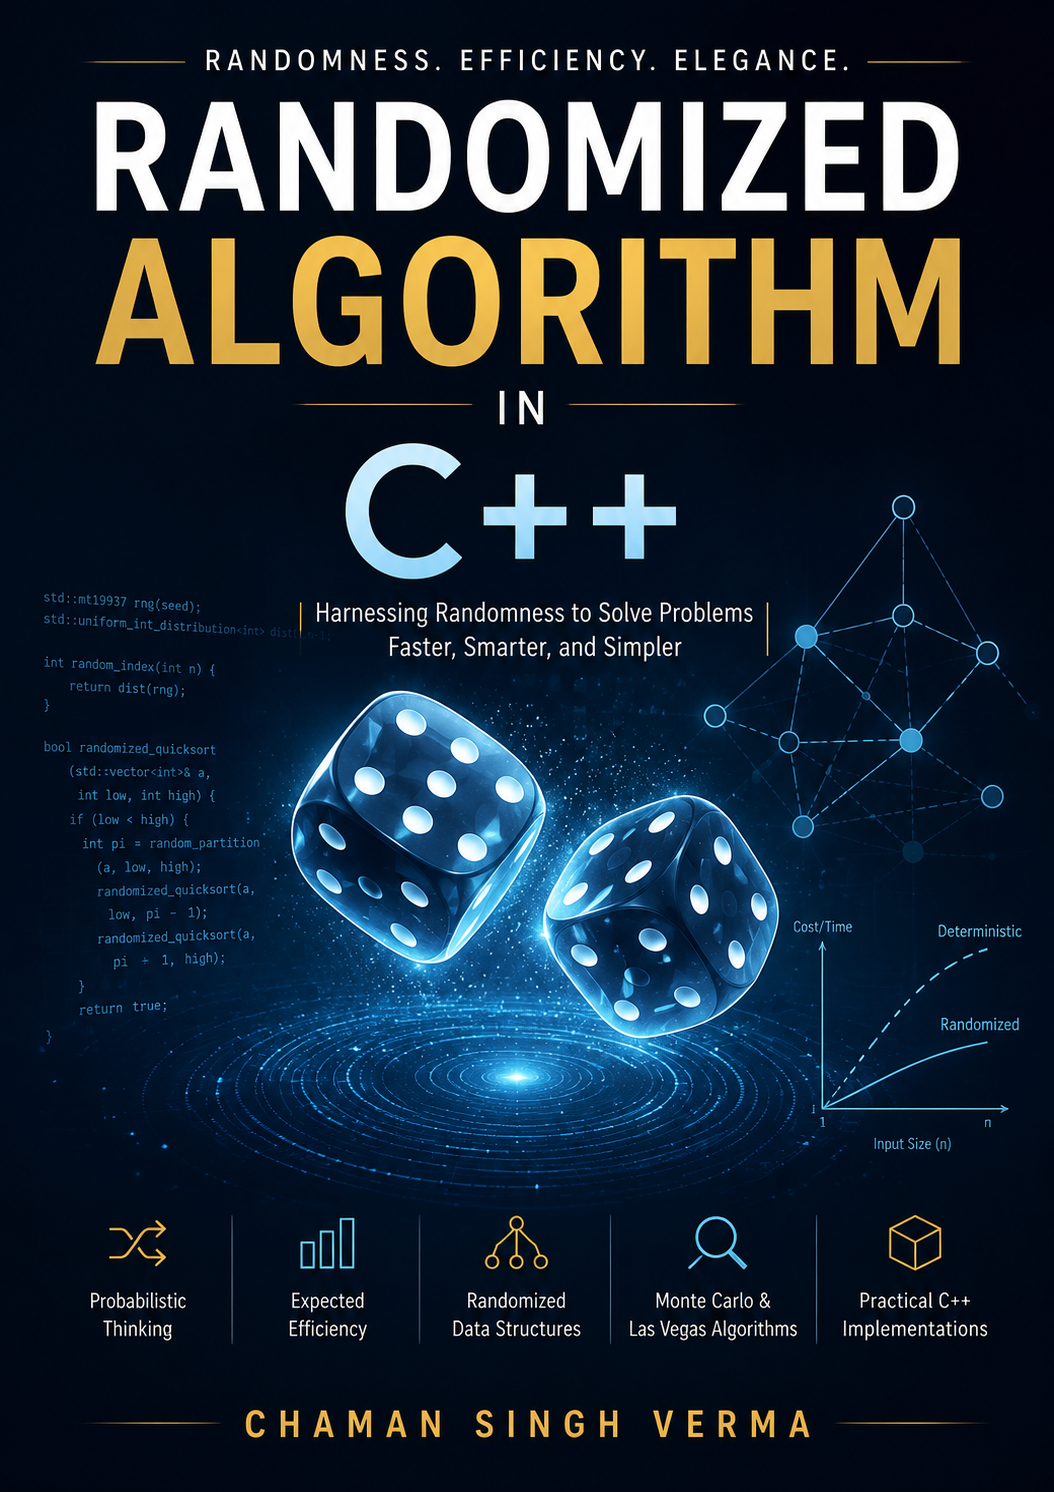
\includegraphics[width=0.85\textwidth]{frontpage.png}
  \vspace*{\fill}
\end{center}
\clearpage
\title{Randomized Algorithms with C++}
\author{Chaman Singh Verma}
\maketitle

%% ============================================================
\chapter*{Preface}
\addcontentsline{toc}{chapter}{Preface}
\markboth{Preface}{Preface}

Randomness is one of the most remarkable and counterintuitive tools in
algorithm design. A small amount of unpredictability, judiciously deployed,
can yield algorithms that are simpler, faster, or both---compared to the
best deterministic alternatives. This book is an invitation to explore the
theory and practice of randomized algorithms, written for advanced
undergraduate students, graduate students, and practitioners who wish to
understand both the mathematical foundations and the engineering realities
of randomized computation.

\paragraph{Scope and approach.}
The book is organized into three parts.  The first part (Chapters~1--6)
develops the probabilistic toolbox: conditional probability, expectation,
tail inequalities, the probabilistic method, and Markov chains.  These
chapters are self-contained and require only a basic familiarity with
discrete mathematics.  The second part (Chapters~7--10) presents
applications in specific domains: algebraic techniques, data structures,
computational geometry, and graph algorithms.  The third part
(Chapters~11--14) addresses advanced topics: approximate counting, parallel
and distributed algorithms, online algorithms, and the number-theoretic
foundations of cryptography.

Throughout the book, algorithms are presented in a dual format: rigorous
mathematical pseudocode alongside complete, compilable C++ implementations.
The C++ code uses modern C++23 features---\texttt{std::ranges}, concepts,
\texttt{std::print}, and the \texttt{<random>} library---and is organized
into header-only files that can be included directly into projects.  Each
implementation is accompanied by a driver program that allows the reader to
verify the theoretical bounds empirically.

\paragraph{Prerequisites.}
Readers are expected to have taken an introductory course in algorithms and
data structures, and to be comfortable with basic probability (sample
spaces, expectation, independence).  The necessary background is reviewed
in Appendix~A.  Familiarity with C++ is assumed for the
implementations; readers who work primarily in another language may skip the
code listings without loss of continuity.

\paragraph{Pedagogical features.}
\begin{itemize}[nosep]
  \item \textbf{Examples and exercises.} Each chapter contains worked
    examples that illustrate key techniques, and a mix of theoretical and
    programming exercises.
  \item \textbf{C++ implementations.} Every major algorithm has a
    corresponding C++ implementation, enabling readers to experiment and
    build intuition.
  \item \textbf{Notes and references.} Each chapter ends with a section
    of historical notes and pointers to the research literature, for
    readers who wish to delve deeper.
  \item \textbf{Appendices.} Appendix~A reviews probability theory,
    Appendix~B covers computational complexity, and Appendix~C surveys the
    modern C++23 features used in the code listings.
\end{itemize}

\paragraph{Acknowledgements.}
I am grateful to the many researchers whose elegant ideas fill these pages.
The theory of randomized algorithms has been shaped by the contributions of
dozens of scholars over the past four decades; I hope this book does justice
to their work.  I thank my students, whose questions and feedback
continually improve my understanding of this material.  Any errors that
remain are, of course, my own responsibility.

\vspace{1em}
\noindent\textbf{Chaman Singh Verma}\\
\noindent 2026

%% ============================================================
\tableofcontents
\clearpage

\hypersetup{pageanchor=true}
\mainmatter


\chapter{Introduction}
\label{ch:introduction}

Algorithms are the engines of computation---systematic procedures that
transform inputs into outputs through a sequence of well-defined steps.
For decades, the gold standard in algorithm design has been
\emph{determinism}: given the same input, a deterministic algorithm always
produces the same output and takes the same time. Yet there exists a large
class of problems for which no efficient deterministic algorithm is known,
and for which the introduction of randomness yields striking improvements in
simplicity, speed, or both. This book is devoted to the theory and practice
of \emph{randomized algorithms}---algorithms that make use of random choices
during their execution.

We begin this chapter by examining why deterministic algorithms, despite
their elegance and predictability, face fundamental limitations. This
motivates the study of randomization as a design principle. We then
discuss random number generation in practice, since every randomized
algorithm ultimately relies on a source of randomness. Next, we gather
the elementary tools from probability theory that will recur throughout
the book: conditional probability, linearity of expectation, and tail
inequalities. Finally, we introduce the main ideas behind randomized
algorithms, covering the two principal paradigms---Las Vegas and Monte
Carlo methods---and illustrating them with concrete examples.

%==========================================================================
\section{Limitations of Deterministic Algorithms}
\label{sec:det-limits}
%==========================================================================

To appreciate the power of randomization, it is essential to understand
where deterministic methods fall short. By ``deterministic algorithm'' we
mean an algorithm whose behavior is completely determined by its input: no
coin flips, no random choices. The running time of a deterministic algorithm
is a function of the input alone.

\subsection{Worst-case complexity is not the full picture}

The traditional framework for analyzing algorithms is \emph{worst-case
complexity}: we measure the running time on the most adversarial input of
size~$n$. This framework has been enormously productive, yielding tight
bounds for many problems (e.g.\ sorting in $O(n \log n)$ time, matrix
multiplication via Strassen's algorithm). However, worst-case analysis can
be overly pessimistic. A deterministic algorithm may be designed to protect
against a pathological input that rarely---or never---occurs in practice.
The resources devoted to handling the worst case may therefore be wasted on
typical inputs.

\subsubsection{Any order versus random order}

A subtle but important distinction concerns the order in which input
elements are presented to an algorithm. This becomes particularly
significant for incremental algorithms that process elements one by one.

\textbf{Any order (adversarial).} When a deterministic incremental algorithm
processes elements~\emph{in any order}, an adversary who knows the algorithm
can choose the order that maximizes the running time or solution cost. For
example, inserting points into a convex hull in worst-case order causes
every insertion to restructure the hull, yielding $O(n^2)$ time. Similarly,
adding elements to a hash table in adversarial order can cause all elements
to collide.

\textbf{Random order.} If the same elements are processed in a uniformly
random permutation, the expected behavior is often dramatically better.
Randomized incremental algorithms exploit this idea: randomizing the order
in which elements are processed turns worst-case inputs into average-case
behavior. For convex hulls, a random insertion order yields $O(n \log n)$
expected time (Section~10.2). For linear programming, the randomized
incremental algorithm of Seidel runs in expected $O(d! n)$ time, which is
linear in~$n$ for fixed dimension~$d$ (Section~10.9).

This principle---\emph{randomizing the order of processing eliminates the
adversary's power to choose a bad order}---is one of the most practical
benefits of randomization in algorithm design. It requires no change to the
input itself, only to the algorithm's scheduling.

\subsection{Problems with no known efficient deterministic solution}

There are problems for which no polynomial-time deterministic algorithm is
known, despite intensive research over many decades. Three categories
illustrate this:

\begin{enumerate}
\item \textbf{NP-hard problems.} The class NP encompasses decision problems
whose YES instances admit short certificates verifiable in polynomial time.
NP-hard problems are at least as hard as every problem in NP. No
polynomial-time algorithm for any NP-hard problem is known, and the
existence of such an algorithm would imply $\mathbf{P} = \mathbf{NP}$.
Famous NP-hard problems include the traveling salesman problem, graph
coloring, and satisfiability (SAT). While no algorithm---deterministic or
randomized---is known to solve these efficiently in general, randomization
yields algorithms that perform well on average or that produce approximate
solutions with provable guarantees (Chapter~12).

\item \textbf{Problems requiring global information.} Some problems seem
inherently difficult for deterministic algorithms because a deterministic
procedure cannot ``explore'' the solution space without being trapped by
adversarial structure. Randomized algorithms can avoid such traps by
exploring the space in an unpredictable fashion.

\item \textbf{Adversarial inputs.} A deterministic algorithm, once its
strategy is known, can be defeated by an adversary who constructs a
worst-case input tailored to exploit the algorithm's predictable behavior.
Randomness removes this vulnerability: an adversary cannot predict the
algorithm's random choices.
\end{enumerate}

\subsection{The adversarial argument}

The idea that an adversary can defeat a deterministic algorithm is
formalized in the following observation. Let $A$ be a deterministic
algorithm for a problem~$\Pi$. Suppose there exists an input $x$ on which
$A$ takes super-polynomial time or produces an incorrect answer. Then the
adversary who knows $A$ can always present $x$ as the input. The
deterministic algorithm has no recourse---it will always behave badly on
$x$.

A randomized algorithm $R$, by contrast, makes random choices during its
execution. Even if the adversary knows the code of $R$ and the input $x$,
the adversary cannot predict the outcome of $R$'s random coins. The best
the adversary can do is ensure that $R$ performs badly on \emph{some} set
of random outcomes; but if $R$ is well designed, the set of ``bad''
outcomes has small probability.

This is the fundamental insight behind the study of randomized algorithms:
\emph{randomness provides immunity against adversarial worst-case inputs.}

\subsection{A concrete example: finding a median}

Consider the problem of finding the median of $n$ numbers. The classical
deterministic algorithm of Blum, Floyd, Pratt, Rivest, and Tarjan solves
this in $O(n)$ time, but the constant hidden in the $O$-notation is
large---the algorithm is complex and rarely used in practice. The
``textbook'' deterministic algorithm based on sorting takes $O(n \log n)$
time.

A simple randomized algorithm achieves $O(n)$ expected time with
remarkable ease: choose a random element as a pivot, partition the array,
and recurse into the side containing the median. The analysis (see
Chapter~4) shows that the expected number of comparisons is at most $4n$.
This algorithm is not only simpler than its deterministic counterpart but
also faster in practice, despite being randomized. (A deterministic
linear-time median algorithm with smaller constants was later discovered,
but the randomized version remains a compelling illustration of the power
of simplicity.)

%==========================================================================
\section{Random Number Generation}
\label{sec:rng}
%==========================================================================

Every randomized algorithm ultimately depends on a source of randomness.
In theoretical analysis we model randomness as an infinite sequence of
independent, uniformly distributed random bits. In practice, we need
algorithms---\emph{pseudorandom number generators} (PRNGs)---that produce
sequences that are ``random enough'' for the application at hand.

\subsection{Pseudorandom number generators}

A PRNG is a deterministic procedure that, given an initial value called a
\emph{seed}, produces a sequence of numbers that appears statistically
random. The sequence is entirely determined by the seed; two runs with the
same seed produce identical sequences.

Modern PRNGs are designed to satisfy two desiderata:
\begin{enumerate}
\item \textbf{Statistical quality:} The output should be indistinguishable
from truly random bits by efficient statistical tests.
\item \textbf{Efficiency:} The generation of each pseudorandom number
should take $O(1)$ time.
\end{enumerate}

The most widely used PRNG in practice is the \emph{Mersenne Twister}
(mt19937), which produces 32-bit pseudorandom integers with a period of
$2^{19937}-1$ and passes most standard statistical tests. C++11 provides
\texttt{std::mt19937} and related distributions via the \texttt{<random>}
header.

\begin{lstlisting}[
  caption={Using the C++ <random> library.},
  label={lst:cpprandom}]
#include <random>
#include <chrono>
#include <iostream>

int main() {
  // Seed from system clock
  unsigned seed = static_cast<unsigned>(
    std::chrono::steady_clock::now()
      .time_since_epoch().count());
  std::mt19937 eng(seed);

  // Uniform integer in [1, 100]
  std::uniform_int_distribution<int> d1(1,100);
  std::cout << "Dice roll: " << d1(eng) << "\n";

  // Uniform real in [0.0, 1.0)
  std::uniform_real_distribution<double> d2(0.0,1.0);
  std::cout << "Uniform:   " << d2(eng) << "\n";

  // Normal distribution
  std::normal_distribution<double> d3(0.0,1.0);
  std::cout << "Gaussian:  " << d3(eng) << "\n";
}
\end{lstlisting}

\subsection{Seeding and reproducibility}

The choice of seed is critical for reproducibility. In scientific
simulations and debugging, it is common to fix the seed so that results can
be reproduced exactly. In production systems, the seed is typically drawn
from a source of entropy (e.g., the system clock, hardware noise, or
\texttt{/dev/urandom} on Unix systems).

Using the same seed with the same PRNG always yields the same sequence.
This property is invaluable for debugging: a bug that manifests on a
particular input can be reproduced by using the same seed.

\subsection{Cryptographically secure PRNGs}

For cryptographic applications, standard PRNGs are insufficient: an attacker
who observes a portion of the output should not be able to predict future
output. Cryptographically secure PRNGs (CSPRNGs) are designed to resist such
attacks. On most systems, \texttt{/dev/urandom} (Unix) or
\texttt{BCryptGenRandom} (Windows) provide CSPRNG output.

\subsection{Weak randomness versus strong randomness}

Not all applications require the same quality of randomness. This
distinction leads to two categories of random sequences.

\subsubsection{Weak random sequences}

A \emph{weak random sequence} is one generated by a simple PRNG with modest
statistical guarantees. Examples include linear congruential generators
(LCGs) and the standard C \texttt{rand()} function. Weak PRNGs are fast and
require little state, but their output has detectable correlations: LCGs
suffer from lattice structure in higher dimensions, and short periods cause
repeat patterns in long runs.

Weak randomness suffices for:
\begin{itemize}
\item \textbf{Monte Carlo integration.} Estimating $\pi$ by sampling points
in a square (Section~1.4.7) converges at $O(1/\sqrt{n})$ regardless of mild
correlations in the samples.
\item \textbf{Randomized incremental algorithms.} Randomizing the insertion
order for convex hulls or Delaunay triangulations (Chapter~10) only requires
that each permutation be approximately equally likely; a weak PRNG suffices.
\item \textbf{Approximate counting.} The Karp--Luby scheme for DNF counting
(Chapter~12) relies on the expectation of indicator variables; the analysis
holds as long as samples are pairwise independent.
\end{itemize}

However, weak randomness can silently invalidate results in applications
that demand uniformity over large state spaces. The RANDU generator (a
notorious LCG from the 1960s) produced triples $(x, W(x), W(W(x)))$ that
all lay on 15 planes in 3D space, corrupting 3D Monte Carlo simulations.

\subsubsection{Strong random sequences}

A \emph{strong random sequence} is one that is statistically
indistinguishable from truly random bits by any polynomial-time test.
The Mersenne Twister (mt19937) with its $2^{19937}-1$ period qualifies for
most non-cryptographic uses. Cryptographically secure PRNGs (CSPRNGs)
provide the strongest guarantee: no polynomial-time adversary can predict
future bits given access to previous output.

Strong randomness is required for:
\begin{itemize}
\item \textbf{Cryptographic protocols.} Key generation, zero-knowledge
proofs, and commitment schemes (Section~15.4) require unpredictability
against an active adversary. A weak PRNG-derived RSA key can be factored.
\item \textbf{Derandomization.} The method of conditional probabilities
(Chapter~6) and pairwise independence (Chapter~4) require true random
bits or provably strong generators.
\item \textbf{Long-running simulations.} Simulations of $10^{12}$ steps
exhaust the period of a 32-bit LCG ($\approx 4\times 10^9$). The
Mersenne Twister's period of $2^{19937}$ is effectively inexhaustible.
\end{itemize}

\subsubsection{Effect on algorithmic guarantees}

A randomized algorithm's theoretical guarantees are proven under the
assumption of true randomness (independent, uniformly distributed bits).
When implemented with a PRNG, the empirical behavior may differ:

\begin{itemize}
\item \textbf{Las Vegas algorithms.} The running time distribution may
shift slightly, but correctness is unaffected: the algorithm always
produces the right answer regardless of the random choices.
\item \textbf{Monte Carlo algorithms.} The error probability may increase
if the PRNG introduces correlations. For example, using \texttt{rand()}
with the Miller--Rabin primality test can misclassify Carmichael numbers
more frequently than the theoretical bound $4^{-k}$.
\item \textbf{Probabilistic method constructions.} The non-constructive
existence proofs (Chapter~6) are unaffected by the PRNG quality, but any
explicit construction derived from derandomization requires strong
randomness.
\end{itemize}

\begin{remark}
In practice, the Mersenne Twister (mt19937) provides sufficient randomness
for nearly all non-cryptographic randomized algorithms discussed in this
book. For cryptographic applications (Chapter~15), always use a CSPRNG from
the operating system's entropy pool.
\end{remark}

\subsection{True randomness versus pseudorandomness}

No sequence produced by a deterministic algorithm is truly random. Every
PRNG is a finite-state machine: given the same seed, it always produces the
same output. The sequence only \emph{appears} random to computational tests.

\subsubsection{Sources of true randomness}

True randomness exists in physical processes:
\begin{itemize}
\item \textbf{Quantum phenomena.} Radioactive decay, photon detection, and
shot noise in semiconductor junctions are fundamentally unpredictable.
Hardware random number generators (HRNGs) exploit these effects.
\item \textbf{Atmospheric noise.} Radio static from lightning strikes
provides a continuous source of entropy.
\item \textbf{Human interaction.} Mouse movements, keyboard timings, and
disk seek latencies are unpredictable enough for seeding PRNGs.
\end{itemize}

Modern operating systems maintain entropy pools fed by hardware interrupts.
On Linux, \texttt{/dev/random} blocks when entropy is low;
\texttt{/dev/urandom} does not but uses a CSPRNG to expand the entropy.

\subsubsection{Practical implications}

For most applications, a well-seeded PRNG is indistinguishable from true
randomness. However, three situations require genuine entropy:
\begin{enumerate}
\item \textbf{Cryptographic key generation.} A key generated by a PRNG with
a predictable seed can be recovered by an adversary.
\item \textbf{Scientific reproducibility.} True randomness cannot reproduce
a simulation; PRNGs with saved seeds enable exact reproducibility.
\item \textbf{Algorithmic fairness.} Lotteries, elections, and audit
selection must resist manipulation. Physical entropy sources (or
public-coin protocols) provide verifiable randomness.
\end{enumerate}

\subsubsection{Buffon's needle: the first Monte Carlo method}

The earliest documented use of randomness to compute a mathematical
constant predates electronic computers by two centuries.

\begin{example}[Buffon's Needle, 1777]
A needle of length~$\ell$ is dropped onto a floor made of parallel wooden
strips of width~$d$ (with $\ell \le d$). What is the probability that the
needle crosses a crack between strips?

Let $y \in [0, d/2]$ be the distance from the needle's midpoint to the
nearest crack, and $\theta \in [0, \pi/2]$ be the acute angle between the
needle and the crack direction. The needle crosses a crack iff
$y \le (\ell/2) \sin\theta$. Assuming $y$ and $\theta$ are independent and
uniformly distributed, the probability is
\[
  p = \frac{2}{\pi} \cdot \frac{\ell}{d}.
\]

By repeating the experiment $n$ times and counting the number $m$ of
crossings, we estimate $\pi$ as
\[
  \pi \approx \frac{2\ell n}{d m}.
\]
\end{example}

Buffon's needle is historically significant for three reasons:
\begin{enumerate}
\item It is the first recorded \emph{Monte Carlo method}---using random
samples to compute a deterministic quantity.
\item It demonstrates that randomness can evaluate integrals without
analytic solution, a principle now central to computational physics,
finance, and Bayesian statistics.
\item The convergence rate $O(1/\sqrt{n})$ is characteristic of all Monte
Carlo methods and sets a fundamental limit on their accuracy.
\end{enumerate}

The needle problem also illustrates a recurring theme: a randomized
algorithm's guarantees rely on the quality of the random source. If the
dropped positions are biased (e.g.\ the dropper unconsciously avoids
cracks), the estimate of $\pi$ becomes systematically wrong. Similarly, a
PRNG with low-period correlations can introduce bias in Monte Carlo
simulations that is invisible to simple statistical tests.

\subsection{Random bits vs.\ random numbers}

Most randomized algorithms require random integers or reals, not raw random
bits. From a theoretical standpoint, this distinction is immaterial: a
random $k$-bit integer can be obtained by sampling $k$ independent random
bits. In practice, PRNGs are often optimized for generating integers in a
given range, which is more efficient than generating raw bits and reducing
modulo.

\begin{remark}
Throughout this book, we assume the availability of a source of independent,
uniformly distributed random bits. When analyzing randomized algorithms, we
study the probability distribution over all possible random outcomes. The
quality of the PRNG used in an implementation affects the empirical
performance but not the theoretical guarantees (which hold for truly random
coins).
\end{remark}

%==========================================================================
\section{Preliminary Mathematics}
\label{sec:prelim-math}
%==========================================================================

The analysis of randomized algorithms draws heavily on elementary
probability theory. In this section we review the tools that will be used
throughout the book. More advanced material (Chernoff bounds, martingales,
the probabilistic method) is introduced in later chapters as needed.

\subsection{Sample spaces and events}

A \emph{probability space} is a triple $(\Omega, \mathcal{F}, \Pr)$,
where $\Omega$ is a set (the \emph{sample space}), $\mathcal{F}$ is a
collection of subsets of $\Omega$ (the \emph{events}), and $\Pr$ is a
probability measure satisfying $\Pr[\Omega]=1$ and countable additivity.

For finite sample spaces, we typically take $\mathcal{F}$ to be all subsets
of $\Omega$ and assign a probability $\Pr[\omega]$ to each outcome
$\omega \in \Omega$ such that $\sum_{\omega \in \Omega} \Pr[\omega] = 1$.
For a uniform distribution, every outcome has probability $1/|\Omega|$.

\subsection{Independence and conditional probability}

Two events $\mathcal{E}_1$ and $\mathcal{E}_2$ are said to be
\emph{independent} if the probability that they both occur is given by
\begin{equation*}
  \Pr[\mathcal{E}_1 \cap \mathcal{E}_2]
  = \Pr[\mathcal{E}_1] \times \Pr[\mathcal{E}_2].
  \tag{1.3}
\end{equation*}
In the more general case where $\mathcal{E}_1$ and $\mathcal{E}_2$ are not
necessarily independent,
\begin{equation*}
  \Pr[\mathcal{E}_1 \cap \mathcal{E}_2]
  = \Pr[\mathcal{E}_1] \times \Pr[\mathcal{E}_2 \mid \mathcal{E}_1],
  \tag{1.4}
\end{equation*}
where $\Pr[\mathcal{E}_1 \mid \mathcal{E}_2]$ denotes the conditional
probability of $\mathcal{E}_1$ given $\mathcal{E}_2$. The chain rule for
probabilities extends this to $k$ events:
\begin{equation*}
  \Pr\!\Bigl[\bigcap_{i=1}^{k} \mathcal{E}_i\Bigr]
  = \Pr[\mathcal{E}_1]
    \times \Pr[\mathcal{E}_2 \mid \mathcal{E}_1]
    \times \Pr[\mathcal{E}_3 \mid \mathcal{E}_1 \cap \mathcal{E}_2]
    \cdots
    \Pr\!\Bigl[\mathcal{E}_k \mid \bigcap_{i=1}^{k-1} \mathcal{E}_i\Bigr].
  \tag{1.5}
\end{equation*}

We used this chain rule in deriving the success probability of Karger's
min-cut algorithm (Eq.~1.1).

\subsection{Expectation and linearity}

The \emph{expected value} (or \emph{mean}) of a discrete random variable
$X$ taking values $x_1, x_2, \ldots$ with probabilities $p_1, p_2,
\ldots$ is
\[
  \mathbb{E}[X] = \sum_{i} x_i \, p_i.
\]

The single most useful tool in the analysis of randomized algorithms is
\emph{linearity of expectation}: for random variables $X_1, X_2, \ldots,
X_n$ (which need not be independent),
\begin{equation*}
  \mathbb{E}\!\Bigl[\sum_{i=1}^{n} X_i\Bigr]
  = \sum_{i=1}^{n} \mathbb{E}[X_i].
  \tag{1.6}
\end{equation*}

\begin{example}[The Sailor Problem]
A ship arrives at a port, and the 40 sailors on board go ashore for
revelry. Later at night, the 40 sailors return to the ship and, in their
state of inebriation, each chooses a random cabin to sleep in. What is the
expected number of sailors sleeping in their own cabins?

Let $X_i$ be 1 if the $i$th sailor chooses her own cabin, and 0 otherwise.
We wish to compute $\mathbb{E}[\sum_{i=1}^{40} X_i]$. By linearity of
expectation, this is $\sum_{i=1}^{40} \mathbb{E}[X_i]$. Since the cabins
are chosen at random, $\mathbb{E}[X_i]=1/40$. Thus the expected number is
$\sum_{i=1}^{40} 1/40 = 1$.
\end{example}

\subsection{Variance and deviations}

The \emph{variance} of a random variable $X$ measures its spread:
\[
  \mathrm{Var}(X) = \mathbb{E}[(X - \mathbb{E}[X])^2]
                  = \mathbb{E}[X^2] - (\mathbb{E}[X])^2.
\]
The \emph{standard deviation} is $\sigma(X) = \sqrt{\mathrm{Var}(X)}$.

\emph{Chebyshev's inequality} bounds the probability that $X$ deviates
significantly from its mean:
\begin{equation*}
  \Pr\bigl[|X - \mathbb{E}[X]| \ge t\bigr]
  \le \frac{\mathrm{Var}(X)}{t^2}.
  \tag{1.7}
\end{equation*}

This inequality will be applied frequently in Chapter~4, where we develop
sharper tail bounds for sums of independent random variables.

\subsection{The union bound}

A simple yet powerful tool is the \emph{union bound} (or \emph{Boole's
inequality}): for events $\mathcal{E}_1, \mathcal{E}_2, \ldots,
\mathcal{E}_n$ (not necessarily independent),
\begin{equation*}
  \Pr\!\Bigl[\bigcup_{i=1}^{n} \mathcal{E}_i\Bigr]
  \le \sum_{i=1}^{n} \Pr[\mathcal{E}_i].
  \tag{1.8}
\end{equation*}
We used the union bound implicitly in the analysis of Karger's algorithm
when bounding the probability that any edge of the min-cut is contracted.

%==========================================================================
\section{The Randomized Approach}
\label{sec:randomized-approach}

A randomized algorithm is an algorithm that can toss coins during its
execution. Formally, we model a randomized algorithm $R$ as a deterministic
algorithm that takes as an additional input a sequence
$r = r_1, r_2, \ldots$ of independent, uniformly distributed random
bits. The output and running time of $R$ are therefore random variables
that depend on $r$.

Randomness serves several distinct roles in algorithm design. We summarize
the four principal motivations before examining each in turn.

\begin{enumerate}
\item \textbf{Improved average-case complexity.} Even when efficient
deterministic algorithms exist, randomization can yield better expected
running time or simpler analysis.
\item \textbf{No efficient deterministic algorithm known.} For certain
problems, randomization provides the only known polynomial-time solution.
\item \textbf{Simplicity.} Randomized algorithms are often dramatically
easier to design, implement, and analyze than their deterministic
counterparts.
\item \textbf{Adversarial immunity.} Randomness shields an algorithm
against worst-case inputs crafted by an adversary who knows the algorithm's
strategy.
\end{enumerate}

\subsection{Improved average-case complexity}

The classical example is sorting. Deterministic comparison-based sorting
achieves $O(n \log n)$ worst-case time, but the algorithms that achieve
this bound (merge sort, heap sort) have overheads that make them slower in
practice than quicksort. Deterministic quicksort, however, has $O(n^2)$
worst-case time. Randomized quicksort resolves this dilemma: it always
produces a correctly sorted array (Las Vegas), yet its expected running
time is $O(n \log n)$, and its practical performance is excellent because
the constant factors are small. The random choice of pivot eliminates the
pathological inputs that defeat deterministic quicksort.

A second example is randomized selection (Section~4.3). The deterministic
median-finding algorithm of Blum et al.\ runs in $O(n)$ time but has large
constants. A simple randomized algorithm achieves $O(n)$ expected time
with much smaller constants by choosing pivots at random.

Further examples include:
\begin{itemize}
\item \textbf{Hash tables.} Universal hashing (Section~9.3) guarantees
$O(1)$ expected time for insertions, deletions, and lookups, even under
adversarial keys. Deterministic hash tables require strong assumptions
about the input distribution or more complex data structures.
\item \textbf{Skip lists.} Skip lists (Section~9.2) achieve $O(\log n)$
expected time for all dictionary operations with a simple randomized
data structure that competes with balanced trees.
\item \textbf{Randomized incremental algorithms.} Building a convex hull
of $n$ points (Section~10.2) in expected $O(n \log n)$ time using
randomized incremental insertion avoids the complex case analysis of
deterministic algorithms like Graham scan.
\item \textbf{Load balancing.} Throwing $m$ balls into $n$ bins uniformly
at random (Chapter~4) yields a maximum load of $O(m/n + \sqrt{m \log n})$.
When $m \approx n$, the maximum load is $O(\log n / \log \log n)$ with
high probability, far smaller than the deterministic worst case.
\end{itemize}

\subsection{No efficient deterministic algorithm known}

Before 2002, no polynomial-time deterministic algorithm was known for
primality testing. The randomized Miller--Rabin test (Chapter~15) runs in
$O(k \log^3 n)$ time with error probability at most $4^{-k}$, making it the
method of choice for decades. The deterministic AKS algorithm, discovered
in 2002, runs in $O(\log^{7.5} n)$ time but is significantly slower in
practice.

Further examples include:
\begin{itemize}
\item \textbf{Polynomial identity testing.} The Schwartz--Zippel lemma
(Section~8.2) provides a randomized algorithm for testing whether a
polynomial is identically zero that is dramatically faster than any
known deterministic method.
\item \textbf{Interactive proof systems.} The class $\mathbf{IP}$ equals
$\mathbf{PSPACE}$ only when randomness and interaction are both allowed
(Section~8.8). Without randomness, interactive proofs collapse to
$\mathbf{NP}$.
\item \textbf{Approximate counting.} Counting the number of satisfying
assignments to a DNF formula (Section~12.2) admits a fully polynomial
randomized approximation scheme, while no deterministic approximation
scheme with comparable guarantees is known.
\item \textbf{Perfect matching in parallel.} Finding a perfect matching
in a graph can be done in $\mathbf{RNC}$ (randomized NC) using the
Isolating Lemma (Section~13.4). No $\mathbf{NC}$ algorithm (deterministic
polylogarithmic-time parallel) is known.
\end{itemize}

\subsection{Simplicity}

Karger's min-cut algorithm (Section~1.4.2) is a striking illustration. The
deterministic algorithms for min-cut are based on network flows and require
sophisticated data structures. Karger's randomized algorithm, by contrast,
is a dozen lines of code: repeatedly contract a random edge. The analysis
is elegant and the implementation is trivial.

Further examples include:
\begin{itemize}
\item \textbf{Freivalds' algorithm.} Verifying the product of two $n
\times n$ matrices (Section~8.1) can be done in $O(n^2)$ time with a
randomized algorithm that multiplies a vector by each matrix. The
deterministic $O(n^2)$ verification algorithm requires a complicated
reduction; the randomized version is a few lines of code.
\item \textbf{Luby's maximal independent set.} Luby's algorithm
(Section~13.3) for finding a maximal independent set in a graph is a
simple randomized parallel algorithm that runs in $O(\log n)$ rounds.
Deterministic parallel algorithms for MIS are significantly more complex.
\item \textbf{Randomized incremental construction.} Deterministic
algorithms for problems like convex hull, Delaunay triangulation, and
linear programming are often complex, requiring careful case analysis.
The randomized incremental approach (Chapter~10) replaces this complexity
with a simple random sampling strategy.
\item \textbf{Tree data structures.} Random treaps and skip lists
(Sections~8.1--8.2) provide simple alternatives to balanced binary search
trees, replacing rotation invariants with randomization.
\end{itemize}

\subsection{Adversarial immunity}

An adversary who knows a deterministic algorithm's code can construct a
worst-case input tailored to exploit its predictable behavior. Randomness
removes this vulnerability: the adversary cannot predict the algorithm's
random choices.

Further examples include:
\begin{itemize}
\item \textbf{Online paging.} No deterministic online algorithm can achieve
a competitive ratio better than $k$ for $k$-page caching. The randomized
marking algorithm (Section~14.1) achieves $O(\log k)$ competitive ratio
against an oblivious adversary.
\item \textbf{Load balancing.} When jobs are assigned to machines by random
choice, the maximum load on any machine is concentrated near the average,
regardless of the job sizes---no adversary can force a bad assignment.
\item \textbf{Byzantine agreement.} Deterministic Byzantine agreement
requires $n \ge 3t+1$ processors to tolerate $t$ faults. Randomized
Byzantine agreement (Section~13.6) can tolerate $t < n/3$ faults with
expected constant-round protocols, circumventing the deterministic lower
bound.
\item \textbf{Quicksort.} Deterministic quicksort is vulnerable to an
adversary who supplies a pre-sorted array, causing $O(n^2)$ behavior.
Randomized quicksort eliminates this attack by choosing pivots randomly.
\item \textbf{Routing on the hypercube.} The randomized oblivious routing
algorithm for the hypercube (Section~5.2) achieves $O(\log n)$ expected
delay for any permutation, while deterministic oblivious routing can
require $\Omega(\sqrt{n})$ delay for some permutations.
\end{itemize}

\subsection{Las Vegas and Monte Carlo algorithms}

Randomized algorithms differ in the nature of their randomness.

\begin{definition}[Las Vegas Algorithm]
A \emph{Las Vegas algorithm} is a randomized algorithm that always produces
the correct output. Its running time is a random variable, and we
characterize it by its expected value.
\end{definition}

\begin{definition}[Monte Carlo Algorithm]
A \emph{Monte Carlo algorithm} is a randomized algorithm that may produce an
incorrect output with some small probability. Its running time is typically
a deterministic bound (e.g., polynomial in the input size).
\end{definition}

Monte Carlo algorithms for decision problems (problems with YES/NO answers)
come in two flavors:
\begin{itemize}
\item \textbf{One-sided error:} The algorithm may err only when it outputs
NO (or only when it outputs YES), but never in the other case.
\item \textbf{Two-sided error:} The algorithm may err regardless of the
correct answer.
\end{itemize}

A Las Vegas algorithm is a special case of a Monte Carlo algorithm with
error probability zero. Conversely, whenever solutions can be verified
efficiently, a Monte Carlo algorithm can be converted into a Las Vegas
algorithm by repeating and checking (see Exercise~1.2 below).

\subsection{The min-cut algorithm: a first example}

We now illustrate the power of randomization with a beautiful algorithm for
the min-cut problem. Let $G$ be a connected, undirected multigraph with $n$
vertices. A \emph{cut} in $G$ is a set of edges whose removal disconnects
$G$. A \emph{min-cut} is a cut of minimum cardinality.

The following randomized algorithm, due to Karger, is disarmingly simple.
We repeat the following step: pick an edge uniformly at random and merge the
two vertices at its endpoints. If there are several edges between some pairs
of newly formed vertices, retain them all. Edges between vertices that are
merged are removed, so that there are never any self-loops. We refer to this
process of merging the two endpoints of an edge into a single vertex as the
\emph{contraction} of that edge. With each contraction, the number of
vertices decreases by one. The crucial observation is that an edge
contraction does not reduce the min-cut size: every cut in the graph at any
intermediate stage is a cut in the original graph. The algorithm continues
the contraction process until only two vertices remain; the set of edges
between these two vertices is output as a candidate min-cut.

\begin{figure}[htbp]
\centering
\begin{tikzpicture}[scale=0.8,
  every node/.style={circle,draw,minimum size=8mm}]
  \node (1) at (0,1)   {1};
  \node (2) at (1.5,1) {2};
  \node (3) at (0.75,2){3};
  \node (4) at (0,0)   {4};
  \node (5) at (1.5,0) {5};
  \draw (1)--(2); \draw (1)--(3); \draw (1)--(4);
  \draw (2)--(3); \draw (2)--(5); \draw (3)--(4);
  \draw (3)--(5); \draw (4)--(5);
  \node at (0.75,-0.8){\small (a) Original graph};

  \node (12) at (4,1)   {$\{1,2\}$};
  \node (3b) at (4.75,2){3};
  \node (4b) at (4,0)   {4};
  \node (5b) at (4.75,0){5};
  \draw (12)--(3b); \draw (12)--(4b); \draw (12)--(5b);
  \draw (3b)--(4b); \draw (3b)--(5b); \draw (4b)--(5b);
  \node at (4.375,-0.8){\small (b) After contracting $(1,2)$};
\end{tikzpicture}
\caption{A step in the min-cut algorithm; the effect of contracting
  edge $e=(1,2)$ is shown.}
\label{fig:contraction}
\end{figure}

Does this algorithm always find a min-cut? No---it may err. But we can
bound the probability of error. Let $k$ be the min-cut size. We fix our
attention on a particular min-cut $C$ with $k$ edges. Clearly $G$ has at
least $kn/2$ edges; otherwise there would be a vertex of degree less than
$k$, and its incident edges would be a min-cut of size less than $k$.

Let $e_i$ denote the event of not picking an edge of $C$ at the $i$th step,
for $1 \le i \le n-2$. The probability that the edge randomly chosen in the
first step is in $C$ is at most $k/(nk/2)=2/n$, so that $\Pr[e_1] \ge
1-2/n$. Assuming that $e_1$ occurs, during the second step there are at
least $k(n{-}1)/2$ edges, so the probability of picking an edge in $C$ is at
most $2/(n{-}1)$, so that $\Pr[e_2 \mid e_1] \ge 1-2/(n{-}1)$. At the $i$th
step, the number of remaining vertices is $n-i+1$. The min-cut size is still
at least~$k$, so the graph has at least $k(n{-}i{+}1)/2$ edges. Thus,
$\Pr[e_i \mid \bigcap_{j=1}^{i-1} e_j] \ge 1-2/(n{-}i{+}1)$.

The probability that no edge of $C$ is ever picked is
\begin{equation*}
  \Pr\!\Bigl[\bigcap_{i=1}^{n-2} e_i\Bigr]
  = \prod_{i=1}^{n-2}\Bigl(1-\frac{2}{n-i+1}\Bigr)
  = \frac{2}{n(n-1)}.
  \tag{1.1}
\end{equation*}

The probability of discovering a particular min-cut is therefore at least
$2/n^2$. To reduce the failure probability, we repeat the algorithm
$n^2/2$ times, making independent random choices each time. The probability
that a min-cut is not found in any attempt is at most
\begin{equation*}
  \Bigl(1-\frac{2}{n^2}\Bigr)^{n^2/2} < \frac{1}{e}.
  \tag{1.2}
\end{equation*}

Further repetitions make the failure probability arbitrarily small---the
only consideration being that repetitions increase running time. Note the
extreme simplicity of this randomized algorithm compared to the
deterministic algorithms for min-cut, which are based on network flows and
are considerably more complex.

\begin{exercise}
Suppose that at each step of the min-cut algorithm, instead of choosing a
random edge for contraction we choose two vertices at random and coalesce
them into a single vertex. Show that there are inputs on which the
probability that this modified algorithm finds a min-cut is exponentially
small.
\end{exercise}

%% ----- C++ : Min-Cut -----
\subsection{C++ Implementation}

The following implementation demonstrates Karger's algorithm.  A multigraph
is represented with weighted adjacency lists; the weight of edge $(u,v)$
equals its multiplicity.

\begin{lstlisting}[
  caption={Graph data structure for the min-cut algorithm.},
  label={lst:graph}]
#include <vector>
#include <unordered_map>
#include <algorithm>
#include <numeric>
#include <climits>
#include <random>
#include <chrono>
#include <iostream>
#include <cmath>

class RandomEngine {
public:
  static RandomEngine& instance() {
    static RandomEngine e; return e;
  }
  int uniform_int(int lo, int hi) {
    return std::uniform_int_distribution<int>(lo,hi)(eng_);
  }
  double uniform_real(double lo=0,double hi=1) {
    return std::uniform_real_distribution<double>(lo,hi)(eng_);
  }
private:
  RandomEngine()
    : eng_(std::chrono::steady_clock::now()
           .time_since_epoch().count()) {}
  std::mt19937 eng_;
};

struct Graph {
  int n;
  std::unordered_map<int,
    std::unordered_map<int,int>> adj;
  explicit Graph(int n) : n(n) {}
  void add_edge(int u, int v, int c=1) {
    adj[u][v]+=c; adj[v][u]+=c;
  }
  int edge_count() const {
    int t=0;
    for (auto& [u,nb] : adj)
      for (auto& [v,w] : nb)
        if (u<v) t+=w;
    return t;
  }
};
\end{lstlisting}

\begin{lstlisting}[
  caption={Karger's min-cut algorithm.},
  label={lst:karger}]
void contract(auto& adj, int u, int v) {
  for (auto& [w,wt] : adj[v])
    if (w!=u) { adj[u][w]+=wt; adj[w][u]+=wt; }
  adj.erase(v);
  for (auto& [_,nb] : adj) nb.erase(v);
  adj[u].erase(u);            // remove self-loops
}

int karger_min_cut(Graph& g) {
  auto adj = g.adj;
  std::vector<int> vs(g.n);
  std::iota(vs.begin(), vs.end(), 0);
  while (vs.size()>2) {
    // collect all edges (with multiplicity)
    std::vector<std::pair<int,int>> E;
    for (auto& [u,nb] : adj)
      for (auto& [v,w] : nb)
        if (u<v)
          for (int i=0;i<w;i++) E.push_back({u,v});
    if (E.empty()) break;
    auto [u,v] = E[RandomEngine::instance()
                        .uniform_int(0,E.size()-1)];
    contract(adj,u,v);
    vs.erase(std::remove(vs.begin(),vs.end(),v),
             vs.end());
  }
  return vs.size()==2 ? adj[vs[0]][vs[1]] : 0;
}

int karger_repeated(Graph& g, int T) {
  int best = INT_MAX;
  for (int t=0;t<T;t++)
    best = std::min(best, karger_min_cut(g));
  return best;
}
\end{lstlisting}

\begin{lstlisting}[
  caption={Driver: empirical verification of the theoretical bounds.},
  label={lst:mincut_demo}]
int main() {
  Graph g(5);
  g.add_edge(0,1); g.add_edge(0,2); g.add_edge(0,3);
  g.add_edge(1,2); g.add_edge(1,3); g.add_edge(2,3);
  g.add_edge(2,4); g.add_edge(3,4);

  int n=g.n, T=(n*n)/2;
  std::cout<<"Single trial : "<<karger_min_cut(g)<<"\n";
  std::cout<<T<<" trials     : "<<karger_repeated(g,T)<<"\n";

  double p=2.0/(n*(n-1));
  std::cout<<"P(success) >= 2/n(n-1) = "<<p<<"\n";
  std::cout<<"P(failure in "<<T<<" trials) <= "
           <<std::pow(1-p,T)<<"\n";
  std::cout<<"1/e = "<<1.0/std::exp(1.0)<<"\n";
}
\end{lstlisting}

\paragraph{Complexity.}
Each trial of the algorithm runs in $O(n^2)$ time with the adjacency-map
representation.  With $n^2/2$ trials the total expected running time is
$O(n^4)$.

%% ----- C++ : Las Vegas -----
\subsection{C++ Implementation: Randomized QuickSort}

Randomized QuickSort is the canonical Las Vegas algorithm: it always
produces a correctly sorted array, yet its running time is a random variable
with $\mathbb{E}[T(n)]=O(n\log n)$.

\begin{lstlisting}[
  caption={Randomized QuickSort---a Las Vegas algorithm.},
  label={lst:quicksort}]
int partition(std::vector<int>& a, int lo, int hi) {
  int pi = RandomEngine::instance().uniform_int(lo,hi);
  std::swap(a[pi], a[hi]);
  int pivot = a[hi], i = lo-1;
  for (int j=lo; j<hi; j++)
    if (a[j]<=pivot) std::swap(a[++i], a[j]);
  std::swap(a[i+1], a[hi]);
  return i+1;
}

void rand_quicksort(std::vector<int>& a,int lo,int hi){
  if (lo<hi) {
    int p = partition(a,lo,hi);
    rand_quicksort(a,lo,p-1);
    rand_quicksort(a,p+1,hi);
  }
}
\end{lstlisting}

%% ----- C++ : Monte Carlo -----
\subsection{C++ Implementation: Monte Carlo---Estimating \texorpdfstring{$\pi$}{pi}}

The following Monte Carlo algorithm estimates $\pi$ by sampling.  It has
two-sided error: the estimate may be too high or too low, but the error
decreases as $O(1/\sqrt{n})$.

\begin{lstlisting}[
  caption={Monte Carlo estimation of $\pi$ (two-sided error).},
  label={lst:pi}]
double estimate_pi(int n) {
  int inside = 0;
  for (int i=0;i<n;i++) {
    double x = RandomEngine::instance()
                   .uniform_real(-1,1);
    double y = RandomEngine::instance()
                   .uniform_real(-1,1);
    if (x*x+y*y<=1.0) inside++;
  }
  return 4.0*inside/n;
}
\end{lstlisting}

\begin{table}[htbp]
\centering
\begin{tabular}{rrr}
\toprule
\textbf{Samples} & \textbf{Estimate} & \textbf{Error} \\
\midrule
    100 & 3.12000 & 0.02159 \\
  1\,000 & 3.14400 & 0.00241 \\
  10\,000 & 3.13840 & 0.00319 \\
 100\,000 & 3.14076 & 0.00083 \\
  \bottomrule
\end{tabular}
\caption{Typical output of the $\pi$ estimator.}
\end{table}

%% ----- C++ : MC $\to$ LV -----
\subsection{Converting Between Las Vegas and Monte Carlo}

A Las Vegas algorithm can be converted to a Monte Carlo algorithm by
truncation.  If the Las Vegas algorithm has expected running time
$T(n)$, run it for $2T(n)$ steps and output an arbitrary default
answer if it has not finished.  By Markov's inequality, the
probability of premature truncation is at most~$1/2$, so the resulting
Monte Carlo algorithm errs with probability at most~$1/2$ and always
runs in $O(T(n))$ time.  Conversely, when solutions can be
\emph{verified} efficiently, a Monte Carlo algorithm can be turned
into a Las Vegas algorithm by repeating until verification succeeds.

\begin{lstlisting}[
  caption={Monte Carlo $\to$ Las Vegas via verification.},
  label={lst:conversion}]
// Monte Carlo: correct w.p.~2/3
std::pair<int,bool> mc(int x) {
  bool ok = RandomEngine::instance()
                 .uniform_real() < 2.0/3.0;
  return ok ? std::make_pair(2*x,true)
            : std::make_pair(3*x,false);
}

bool verify(int x, int r) { return r==2*x; }

// Las Vegas wrapper
std::pair<int,int> mc_to_lv(int x) {
  int tries=0;
  while (true) {
    tries++;
    auto [r,ok] = mc(x);
    if (verify(x,r)) return {r,tries};
  }
}
\end{lstlisting}

\begin{remark}
If the single-trial success probability is~$p$, the number of independent
trials until the first success follows a \emph{geometric distribution} with
mean~$1/p$.  Hence the expected running time of the Las Vegas wrapper is
$(T(n)+t(n))/p$.
\end{remark}

%==========================================================================
\chapter{Fundamentals}
\label{ch:fundamentals}

In this chapter we develop fundamental mathematical tools and computational
models that underpin the randomized algorithms studied in the remainder of
the book. We begin with the construction of binary planar partitions,
illustrating linearity of expectation with a geometric application. We then
study a probabilistic recurrence that arises in the analysis of selection
and other divide-and-conquer algorithms. Finally, we review the computation
model and complexity classes that provide the formal framework for our
discussions throughout the book.

\section{Binary Planar Partitions}
\label{sec:bpp}
%==========================================================================

We now illustrate linearity of expectation with another application. Given a
set $S=\{s_1,s_2,\ldots,s_n\}$ of non-intersecting line segments in the
plane, we wish to construct a \emph{binary planar partition}---a binary
tree in which each node is associated with a region of the plane, and each
region contains at most one line segment. Such partitions have applications
to hidden-line elimination in computer graphics.

%% ----- Binary Planar Partitions -----
\subsection{Binary Planar Partitions}

Our next illustration is the construction of a binary planar partition of a
set of $n$ disjoint line segments in the plane, a problem with applications
to computer graphics.  A binary planar partition consists of a binary tree
together with some additional information, as described below.  Every internal
node of the tree has two children.  Associated with each node $v$ of the tree
is a region $r(v)$ of the plane.  Associated with each internal node $v$ of
the tree is a line $\ell(v)$ that intersects $r(v)$.  The region
corresponding to the root is the entire plane.  The region $r(v)$ is
partitioned by $\ell(v)$ into two regions $r_1(v)$ and $r_2(v)$, which are
the regions associated with the two children of~$v$.  Thus, any region $r$ of
the partition is bounded by the partition lines on the path from the root to
the node corresponding to $r$ in the tree.

Given a set $S=\{s_1,s_2,\ldots,s_n\}$ of non-intersecting line segments
in the plane, we wish to find a binary planar partition such that every
region in the partition contains at most one line segment (or a portion of
one line segment).  Notice that the definition allows us to divide an input
line segment $s_i$ into several segments $s_{i1},s_{i2},\ldots$, each of
which lies in a different region.

\begin{exercise}
Show that there exists a set of line segments for which no binary planar
partition can avoid breaking up some of the segments into pieces, if each
segment is to lie in a different region of the partition.
\end{exercise}

Binary planar partitions have two applications in computer graphics.  Here,
we describe one of them, the problem of hidden line elimination.  The second
application has to do with the constructive solid geometry (or CSG)
representation of a polyhedral object.

In rendering a scene on a graphics terminal, we are often faced with a
situation in which the scene remains fixed, but it is to be viewed from
several directions.  The hidden line elimination problem is the following:
having adopted a viewpoint and a direction of viewing, we want to draw only
the portion of the scene that is visible, eliminating those objects that are
``obscured by other objects'' in front of them relative to the viewpoint.

One approach uses a binary partition tree.  Once the scene has been decomposed
into line segments, we construct a binary planar partition tree for it.  Now,
given the direction of viewing, we use an idea known as the \emph{painter's
algorithm} to render the scene: first draw the objects that are furthest
``behind,'' and then progressively draw the objects that are in front.

The time it takes to render the scene depends on the size of the binary
planar partition tree.  We therefore wish to construct a binary planar
partition that is as small as possible.  Because the construction of the
partition can break some of the input segments $s_i$ into smaller pieces, the
size of the partition need not be~$n$; in fact, it is not clear that a
partition of size $O(n)$ always exists.

For a line segment $s$, let $\ell(s)$ denote the line obtained by extending
(if necessary) $s$ on both sides to infinity.  For the set
$S=\{s_1,s_2,\ldots,s_n\}$ of line segments, a simple and natural class of
partitions is the set of \emph{autopartitions}, which are formed by only
using lines from the set $\{\ell(s_1),\ell(s_2),\ldots,\ell(s_n)\}$ in
constructing the partition.

\begin{algorithm}[htbp]
\caption{RandAuto}
\label{alg:randauto}
\begin{algorithmic}[1]
\State \textbf{Input:} A set $S=\{s_1,\ldots,s_n\}$ of non-intersecting
  line segments.
\State \textbf{Output:} A binary autopartition $P_\pi$ of $S$.
\State Pick a permutation $\pi$ of $\{1,2,\ldots,n\}$ uniformly at random.
\While{a region contains more than one segment}
  \State Cut it with $\ell(s_i)$ where $i$ is first in $\pi$ such that
    $s_i$ cuts that region.
\EndWhile
\end{algorithmic}
\end{algorithm}

\begin{theorem}
\label{thm:partition}
The expected size of the autopartition produced by RandAuto is $O(n\log n)$.
\end{theorem}

\begin{proof}
For line segments $u$ and $v$, define $\operatorname{index}(u,v)$ to be~$i$
if $\ell(u)$ intersects $i{-}1$ other segments before hitting $v$, and
$\operatorname{index}(u,v)=\infty$ if $\ell(u)$ does not hit $v$.  Since a
segment $u$ can be extended in two directions, it is possible that
$\operatorname{index}(u,v)=\operatorname{index}(u,w)$ for two different
lines $v$ and $w$.

Let us denote by $u\dashv v$ the event that $\ell(u)$ cuts $v$ in the
constructed partition.  Let $\operatorname{index}(u,v)=i$, and let
$u_1,u_2,\ldots,u_{i-1}$ be the segments that $\ell(u)$ intersects before
hitting~$v$.  The event $u\dashv v$ happens only if $u$ occurs before any
of $\{u_1,u_2,\ldots,u_{i-1},v\}$ in the randomly chosen permutation
$\pi$.  The probability that this happens is $1/(i+1)$.

Let $C_{u,v}$ be an indicator variable that is 1 if $u\dashv v$ and 0
otherwise; clearly,
$\mathbb{E}[C_{u,v}]=\Pr[u\dashv v]\le 1/(\operatorname{index}(u,v)+1)$.
The size of $P_\pi$ equals $n$ plus the number of intersections due to cuts.
Thus, its expectation is
$n+\mathbb{E}[\sum_u\sum_v C_{u,v}]$ and by linearity of expectation this
equals
\begin{equation*}
  n + \sum_u \sum_v \Pr[u\dashv v]
  \le n + \sum_u \sum_v
    \frac{1}{\operatorname{index}(u,v)+1}.
  \tag{2.1}
\end{equation*}

For any line segment $u$ and any finite positive integer $i$, there are at
most two vertices $v$ and $w$ such that $\operatorname{index}(u,v)$ and
$\operatorname{index}(u,w)$ equal~$i$.  This is because the extension of the
segment $u$ along either of the two possible directions will meet any other
line segment at most once.  Thus, in each of the two directions, there is a
total ordering on the points of intersection with other segments and the
index values increase monotonically.  This implies that
\begin{equation*}
  \sum_{v\ne u} \frac{1}{\operatorname{index}(u,v)+1}
  \le \sum_{i=1}^{n-1} \frac{2}{i+1}
  = O(\log n).
  \tag{2.2}
\end{equation*}

Combining this with~(2.1) implies that the expected size of $P_\pi$ is
bounded above by $n+O(n\log n)$, which is $O(n\log n)$.
\end{proof}

Note that in computing the expected number of intersections, we only made
use of linearity of expectation.  We do not require any independence between
the events $u\dashv v$ and $u\dashv w$, for segments $u$, $v$, and~$w$.
Indeed, these events need not be independent in general.

One way of interpreting Theorem~\ref{thm:partition} is as follows: since the
expected size of the binary planar partition constructed by the algorithm is
$O(n\log n)$ on any input, there must exist a binary autopartition of size
$O(n\log n)$ for every input.  This follows from the simple fact that any
random variable assumes at least one value that is no greater than its
expectation.  Thus we have used a \emph{probabilistic argument} to assert
that a combinatorial object---in this case a binary autopartition of size
$O(n\log n)$---exists with absolute certainty rather than with some
probability.  This is an example of the \emph{probabilistic method} in
combinatorics.  We will study the probabilistic method in greater detail in
Chapter~6.

%% ----- C++ : BPP -----
\subsubsection*{C++ Implementation}

\begin{lstlisting}[
  caption={RandAuto for binary planar partitions.},
  label={lst:bpp}]
struct Seg { double x1,y1,x2,y2; int id; };

bool intersect(const Seg& a, const Seg& b) {
  auto o=[](double px,double py,
            double qx,double qy,
            double rx,double ry){
    double v=(qy-py)*(rx-qx)-(qx-px)*(ry-qy);
    return std::abs(v)<1e-10?0:(v>0?1:2);
  };
  return o(a.x1,a.y1,a.x2,a.y2,b.x1,b.y1)
        !=o(a.x1,a.y1,a.x2,a.y2,b.x2,b.y2)
      && o(b.x1,b.y1,b.x2,b.y2,a.x1,a.y1)
        !=o(b.x1,b.y1,b.x2,b.y2,a.x2,a.y2);
}

// Build autopartition recursively
// segs: remaining segments in this region
// Returns number of leaf nodes (partition size)
int rand_auto(std::vector<Seg*>& segs) {
  if (segs.empty()) return 0;
  if (segs.size()==1) return 1;       // leaf
  std::vector<int> p(segs.size());
  std::iota(p.begin(),p.end(),0);
  std::shuffle(p.begin(),p.end(),
    std::mt19937(std::random_device()()));
  Seg* cut = segs[p[0]];             // random pivot
  std::vector<Seg*> L,R;
  for (size_t i=1;i<segs.size();i++) {
    if (intersect(*cut,*segs[i]))
      { L.push_back(segs[i]); R.push_back(segs[i]); }
    else {
      double dx=cut->x2-cut->x1;
      double dy=cut->y2-cut->y1;
      double cross=dx*(segs[i]->y1-cut->y1)
                  -dy*(segs[i]->x1-cut->x1);
      (cross>=0?L:R).push_back(segs[i]);
    }
  }
  return rand_auto(L)+rand_auto(R);
}
\end{lstlisting}

%==========================================================================
\section{A Probabilistic Recurrence}
\label{sec:recurrence}
%==========================================================================

Frequently, we express a random variable of interest as a recurrence in
terms of other random variables.  In this section, we study one such
situation using the Find algorithm analyzed in detail in Problem~1.9.  The
material in this section, although useful, is not an essential prerequisite
for subsequent topics and may be omitted in the first reading.

The Find algorithm for selecting the $k$th smallest of a set $S$ of $n$
elements works as follows.  We pick a random element $y$ and partition
$S\setminus\{y\}$ into two sets $S_1$ and $S_2$ (elements smaller and larger
than~$y$ respectively) as in RandQS.  Suppose $|S_1|=k-1$; then $y$ is the
desired element and we are done.  Otherwise, if $|S_1|>k$, we recursively
find the $k$th smallest element of $S_1$; else we recursively find the
$(k-|S_1|-1)$th smallest element in~$S_2$.

The expected number of comparisons made by the Find algorithm is the subject
of Problem~1.9.  Suppose instead that we were to ask the following question:
what is the expected number of times we make the recursive call in the
algorithm?  Equivalently, what is the expected number of times we pick a
random element in the algorithm?  While this question may not be especially
important for the Find algorithm, it is the kind of question that arises in
the analysis of a number of parallel and geometric algorithms.  Intuitively,
we expect that the size of the residual problem in the Find algorithm is
divided by a constant factor at each recursive level, so that we expect that
the number of recursive invocations is $O(\log n)$.  Below, we show that
this intuition can be formalized in a general setting.

Let $g(x)$ be a monotone non-decreasing function from the positive reals to
the positive reals.  Consider a particle whose position changes at discrete
time steps and is always at a positive integer.  If the particle is currently
at position $m>1$, it proceeds at the next step to the position $m-X$, where
$X$ is a random variable ranging over the integers $1,\ldots,m-1$.  All we
know about $X$ is that $\mathbb{E}[X]\ge g(m)$, and that $X$ is chosen
independently of the past.  It is clear that the particle will always reach
position~1 and the process terminates in that state.  The interesting
question is, assuming that the particle starts at position~$n$, what is the
expected number of steps before it reaches position~1?

\begin{theorem}
\label{thm:recurrence}
Let $T$ be the random variable denoting the number of steps in which the
particle reaches the position~1.  Then,
$\mathbb{E}[T]\le \displaystyle\int_1^n \frac{dx}{g(x)}$.
\end{theorem}

\begin{proof}
The proof is by induction on $n$; let us suppose the theorem holds for values
of $m$ smaller than $n$.  Let $f(m)=\int_1^m dx/g(x)$ for $m>1$.  We wish
to show that $\mathbb{E}[T]\le f(n)$.

Consider the first step, during which the particle proceeds from position $n$
to position $n-X$, where $X$ is chosen from a distribution for which
$\mathbb{E}[X]\ge g(n)$.  We have
\begin{align}
  \mathbb{E}[T]
  &\le 1 + \mathbb{E}[f(n-X)]
    \tag{1.9}\\
  &= 1 + \mathbb{E}\!\left[\int_{n-X}^{n}\frac{dy}{g(y)}\right]
    \tag{1.10}\\
  &\le 1 + \mathbb{E}\!\left[\frac{X}{g(n)}\right]
    \tag{1.11}\\
  &= 1 + \frac{\mathbb{E}[X]}{g(n)}
    \tag{1.12}\\
  &\le 1 + f(n) - 1 = f(n).
    \tag{1.13}
\end{align}
The inequality~(1.10) follows from the inductive hypothesis applied to
position $n-X$.  The inequality~(1.11) follows from the assumption that $g$
is non-decreasing, so $1/g(y)\le 1/g(n)$ for $y\le n$.  The
inequality~(1.13) follows from the lower bound on $\mathbb{E}[X]$ and the
observation that $f(n)-f(n-X)\ge X/g(n)$.
\end{proof}

\begin{exercise}
If $X$ were to range over all integers having value at most $m-1$ (possibly
including negative integers), how would the statement and proof of
Theorem~\ref{thm:recurrence} change?
\end{exercise}

For the Find algorithm, we can show (following the analysis of Problem~1.9)
that $g(m)\ge m/4$.  We may then apply the above theorem to bound the
expected number of recursive calls to Find by $4\ln n$.

\begin{exercise}
What prevents us from using Theorem~\ref{thm:recurrence} to bound the
expected number of levels of recursion in the RandQS algorithm?
\end{exercise}

%% ----- C++ : Find -----
\subsection{C++ Implementation}

\begin{lstlisting}[
  caption={Randomized Find---selecting the $k$th smallest element.},
  label={lst:find}]
int rand_find(std::vector<int>& a, int k) {
  if (a.size()==1) return a[0];
  int pi = RandomEngine::instance()
               .uniform_int(0,a.size()-1);
  int pivot = a[pi];
  std::vector<int> L,E,G;
  for (int x : a) {
    if      (x<pivot) L.push_back(x);
    else if (x==pivot) E.push_back(x);
    else              G.push_back(x);
  }
  if (k<=(int)L.size())
    return rand_find(L,k);
  else if (k<=(int)(L.size()+E.size()))
    return pivot;
  else
    return rand_find(G,k-L.size()-E.size());
}
\end{lstlisting}

\begin{lstlisting}[
  caption={Empirical measurement of recursion depth.},
  label={lst:find_analysis}]
struct Stats { int calls=0, depth=0; };

int rand_find_analyzed(std::vector<int>& a,int k,
                       int d, Stats& s) {
  s.calls++;
  s.depth = std::max(s.depth,d);
  if (a.size()==1) return a[0];
  int pi = RandomEngine::instance()
               .uniform_int(0,a.size()-1);
  int pivot = a[pi];
  std::vector<int> L,E,G;
  for (int x : a) {
    if      (x<pivot) L.push_back(x);
    else if (x==pivot) E.push_back(x);
    else              G.push_back(x);
  }
  if (k<=(int)L.size())
    return rand_find_analyzed(L,k,d+1,s);
  else if (k<=(int)(L.size()+E.size()))
    return pivot;
  else
    return rand_find_analyzed(G,
      k-L.size()-E.size(),d+1,s);
}

// Typical output for n=1000:
//   Avg recursive calls: ~12
//   Avg max depth:       ~11
//   Theoretical O(log n): ~10
//   Theorem 1.3 bound 4 ln n: ~27
\end{lstlisting}

%==========================================================================
\section{Computation Model and Complexity Classes}
\label{sec:complexity}
%==========================================================================

\subsection{RAMs and Turing Machines}

Following common practice, throughout this book we use the Turing machine
model to discuss complexity-theory issues.  As is common, however, we switch
to the RAM (random access machine) as the model of computation when
describing and analyzing algorithms (except in the study of parallel and
distributed algorithms in Chapter~13, where we define a version of the RAM
model for machines working in parallel).

\begin{definition}
A \emph{deterministic Turing machine} is a quadruple $M=(S,\Sigma,\delta,s)$.
Here $S$ is a finite set of states, of which $s\in S$ is the machine's
initial state.  The machine uses a finite set of symbols, denoted~$\Sigma$;
this set includes special symbols $\mathrm{BLANK}$ and $\mathrm{FIRST}$.  The
function $\delta$ is the transition function, mapping
$S\times\Sigma$ to
$(S\cup\{\mathrm{HALT},\mathrm{YES},\mathrm{NO}\})\times\Sigma\times\{\leftarrow,
\rightarrow,\mathrm{STAY}\}$.
\end{definition}

A \emph{probabilistic Turing machine} is a Turing machine augmented with the
ability to generate an unbiased coin flip in one step.  It corresponds to a
randomized algorithm.

In the RAM model, we have a machine that can perform the following types of
operations involving registers and main memory: input--output operations,
memory--register transfers, indirect addressing, branching, and arithmetic
operations.  Each register or memory location may hold an integer that can be
accessed as a unit, but an algorithm has no access to the representation of
the number.

\begin{proposition}
Any Turing machine computation of length polynomial in the size of the input
can be simulated by a RAM computation of length polynomial in the size of the
input.  Any RAM computation of length polynomial in the size of the input can
be simulated by a Turing machine computation of length polynomial in the size
of the input.
\end{proposition}

\subsection{Complexity Classes}

We now define some basic complexity classes focusing on those involving
randomized algorithms.

\begin{definition}
The class $\mathbf{P}$ consists of all languages $L$ that have a
polynomial-time algorithm $A$ such that for any input $x\in\Sigma^*$,
$x\in L \Rightarrow A(x)$ accepts, and
$x\notin L \Rightarrow A(x)$ rejects.
\end{definition}

\begin{definition}
The class $\mathbf{NP}$ consists of all languages $L$ that have a
polynomial-time algorithm $A$ such that for any input $x\in\Sigma^*$,
$x\in L \Rightarrow \exists\, y\in\Sigma^*: A(x,y)$ accepts, where
$|y|$ is bounded by a polynomial in $|x|$; and
$x\notin L \Rightarrow \forall\, y\in\Sigma^*: A(x,y)$ rejects.
\end{definition}

\begin{definition}
The class $\mathbf{RP}$ (Randomized Polynomial time) consists of all
languages $L$ that have a randomized algorithm $A$ running in worst-case
polynomial time such that for any input $x\in\Sigma^*$,
$x\in L \Rightarrow \Pr[A(x)\text{ accepts}]\ge 1/2$; and
$x\notin L \Rightarrow \Pr[A(x)\text{ accepts}]=0$.
\end{definition}

\begin{definition}
The class $\mathbf{ZPP}$ (Zero-error Probabilistic Polynomial time) is the
class of languages that have Las Vegas algorithms running in expected
polynomial time.
\end{definition}

\begin{definition}
The class $\mathbf{BPP}$ (Bounded-error Probabilistic Polynomial time)
consists of all languages $L$ that have a randomized algorithm $A$ running
in worst-case polynomial time such that for any input $x\in\Sigma^*$,
$x\in L \Rightarrow \Pr[A(x)\text{ accepts}]\ge 3/4$; and
$x\notin L \Rightarrow \Pr[A(x)\text{ accepts}]\le 1/4$.
\end{definition}

\begin{exercise}
Show that $\mathrm{ZPP}=\mathrm{RP}\cap\mathrm{co\text{-}RP}$.
\end{exercise}



%==========================================================================
\addcontentsline{toc}{section}{Notes}
\section*{Notes}
%==========================================================================

The ideas underlying randomized algorithms can be traced back to Monte Carlo
methods used in numerical analysis, statistical physics, and simulation.  In
the context of computability theory, the notion of a probabilistic Turing
machine was proposed by de~Leeuw, Moore, Shannon, and Shapiro~[122] and
further explored in the pioneering work of Rabin~[340] and
Gill~[166].  Berlekamp~[57], Rabin~[341], and Solovay and
Strassen~[382] gave early examples of concrete randomized algorithms.

Our RandQS algorithm is based on Hoare's algorithm~[201].  The min-cut
algorithm of Section~1.2.2, together many variations and
extensions, is due to Karger~[231].  Monte Carlo methods have been popular in
the sciences for over a hundred years.  The classic experiment on
approximating the value of $\pi$ by dropping needles on a sheet of paper with
parallel lines is described in an eighteenth-century paper by
Buffon~[86].  The origin of the modern theory of Monte Carlo methods in the
physical sciences is widely attributed to Ulam, von~Neumann, and
Fermi~[116].  The term \emph{Las Vegas algorithm} was introduced by
Babai~[37].

The material of Section~\ref{sec:bpp} is drawn from Paterson and
Yao~[329].  The Find algorithm described in Section~\ref{sec:recurrence} is
due to Hoare~[200].  Theorem~\ref{thm:recurrence} is given in a paper by
Karp, Upfal, and Wigderson~[250].  Karp~[244] gives a number of additional
results on probabilistic recurrence relations.

The reader is referred to introductory texts on algorithms and complexity
such as those by Aho, Hopcroft, and Ullman~[5,~6] and
Papadimitriou~[326] for more details on the Turing machine model and the
RAM model.  The books by Bovet and Crescenzi~[81] and by
Papadimitriou~[326] contain a more detailed treatment of the complexity
classes described in this chapter.

%==========================================================================
\addcontentsline{toc}{section}{Problems}
\section*{Problems}
%==========================================================================

\begin{exercise}[1.1]
(Due to J.~von~Neumann~[409].)
\begin{enumerate}[label=(\alph*)]
\item Suppose you are given a coin for which the probability of HEADS, say
  $p$, is unknown.  How can you use this coin to generate unbiased (i.e.,
  $\Pr[\text{HEADS}]=\Pr[\text{TAILS}]=1/2$) coin-flips?  Give a scheme for
  which the expected number of flips of the biased coin for extracting one
  unbiased coin-flip is no more than $1/[p(1-p)]$.  (Hint: Consider two
  consecutive flips of the biased coin.)
\item Devise an extension of the scheme that extracts the largest possible
  number of independent, unbiased coin-flips from a given number of flips of
  the biased coin.
\end{enumerate}
\end{exercise}

\begin{exercise}[1.2]
(Due to D.~E.~Knuth and A.~C.-C.~Yao~[264].)
\begin{enumerate}[label=(\alph*)]
\item Suppose you are provided with a source of unbiased random bits.  Explain
  how you will use this to generate uniform samples from the set
  $S=\{0,\ldots,n-1\}$.  Determine the expected number of random bits
  required by your sampling algorithm.
\item What is the worst-case number of random bits required by your sampling
  algorithm?  Consider the case when $n$ is a power of~2, as well as the case
  when it is not.
\item Solve (a) and (b) when, instead of unbiased random bits, you are
  required to use as the source of randomness uniform random samples from the
  set $\{0,\ldots,p-1\}$; consider the case when $n$ is a power of $p$, as
  well as the case when it is not.
\end{enumerate}
\end{exercise}

\begin{exercise}[1.3]
(Due to D.~E.~Knuth and A.~C.-C.~Yao~[264].) Suppose you are provided with
a source of unbiased random bits.  Provide efficient (in terms of expected
running time and expected number of random bits used) schemes for generating
samples from the distribution over the set $\{2,3,\ldots,12\}$ induced by
rolling two unbiased dice and taking the sum of their outcomes.
\end{exercise}

\begin{exercise}[1.4]
\begin{enumerate}[label=(\alph*)]
\item Suppose you are required to generate a random permutation of size $n$.
  Assuming that you have access to a source of independent and unbiased
  random bits, suggest a method for generating random permutations of size
  $n$.  Efficiency is measured in terms of both time and number of random
  bits.  What lower bounds can you prove for this task?
\item Consider the following method for generating a random permutation of
  size $n$.  Pick $n$ random values $X_1,\ldots,X_n$ independently from the
  uniform distribution over the interval $[0,1]$.  Now, the permutation that
  orders the random variables in ascending order is claimed to be a random
  permutation, and it can be determined by sorting the random values.  Is the
  claim correct?  How efficient is this scheme?
\item Consider the following ``lazy'' implementation of the scheme suggested
  in~(b).  The binary representation of the fraction $X_i$ is a sequence of
  unbiased and independent random bits.  At any given stage of the sorting
  algorithm, we would have chosen only as many bits of each $X_i$ as
  necessary to resolve all the comparisons performed up to that point.  When
  comparing $X_i$ to $X_j$, if the current prefixes of their binary
  expansions do not determine the outcome of the comparison, then we extend
  their prefixes by choosing further random bits until this happens.  Compute
  tight bounds on the expected number of random bits used by this
  implementation.
\end{enumerate}
\end{exercise}

\begin{exercise}[1.5]
Consider the problem of using a source of unbiased random bits to generate
samples from the set $S=\{0,\ldots,n-1\}$ such that the element $i$ is
chosen with probability $p_i$.  Show how to perform this sampling using
$O(\log n)$ random bits per sample, regardless of the values of $p_i$.  Use
the result from part~(c) of Problem~1.4.
\end{exercise}

\begin{exercise}[1.6]
Consider a sequence of $n$ flips of an unbiased coin.  Let $H_i$ denote the
absolute value of the excess of the number of HEADS over the number of TAILS
seen in the first $i$ flips.  Define $H=\max_i H_i$.  Show that
$\mathbb{E}[H_i]=\Theta(\sqrt{i})$, and that
$\mathbb{E}[H]=\Theta(\sqrt{n})$.
\end{exercise}

\begin{exercise}[1.7]
Suppose we choose a permutation $\pi$ of the ordered set
$N=\{1,2,\ldots,n\}$ uniformly at random from the space of all permutations
of $N$.  Let $L(\pi)$ denote the length of the longest increasing
subsequence in permutation~$\pi$.
\begin{enumerate}[label=(\alph*)]
\item For large $n$ and some positive constant $c$, prove that
  $\mathbb{E}[L(\pi)]\ge c\sqrt{n}$.
\item Is the bound in~(a) tight?
\end{enumerate}
\end{exercise}

\begin{exercise}[1.8]
Consider adapting the min-cut algorithm of Section~1.2.2 to the
problem of finding an $s$-$t$ min-cut in an undirected graph.  In this
problem, we are given an undirected graph $G$ together with two distinguished
vertices $s$ and $t$.  An $s$-$t$ cut is a set of edges whose removal from
$G$ disconnects $s$ from $t$; we seek an $s$-$t$ cut of minimum cardinality.
As the algorithm proceeds, the vertex $s$ may get amalgamated into a new
vertex as a result of an edge being contracted; we call this vertex the
$s$-vertex (initially the $s$-vertex is $s$ itself).  Similarly, we have a
$t$-vertex.  As we run the contraction algorithm, we ensure that we never
contract an edge between the $s$-vertex and the $t$-vertex.
\begin{enumerate}[label=(\alph*)]
\item Show that there are graphs on which the probability that this algorithm
  finds an $s$-$t$ min-cut is exponentially small.
\item How large can the number of $s$-$t$ min-cuts in an instance be?
\end{enumerate}
\end{exercise}

\begin{exercise}[1.9]
Consider the Find algorithm described in Section~\ref{sec:recurrence} for
selecting the $k$th smallest of a set $S$ of $n$ elements.  Show that the
algorithm finds the $k$th smallest element in $S$ in expected time $O(n)$.
\end{exercise}

\begin{exercise}[1.10]
Consider the setting of Example~1.1 (the Sailor Problem).  Show that the
probability that no sailor returns to her own cabin approaches $1/e$ as the
number of sailors grows large.
\end{exercise}

\begin{exercise}[1.11]
Verify the following inclusions:
$\mathrm{P}\subseteq\mathrm{RP}\subseteq\mathrm{NP}
  \subseteq\mathrm{PSPACE}\subseteq\mathrm{EXP}\subseteq\mathrm{NEXP}$.
It is not known whether these inclusions are strict.
\end{exercise}

\begin{exercise}[1.12]
Verify the following inclusions:
$\mathrm{RP}\subseteq\mathrm{BPP}\subseteq\mathrm{PP}$.
It is not known whether these inclusions are strict.
\end{exercise}

\begin{exercise}[1.13]
Show that $\mathrm{PP}=\mathrm{co\text{-}PP}$ and
$\mathrm{BPP}=\mathrm{co\text{-}BPP}$.
\end{exercise}

\begin{exercise}[1.14]
Show that $\mathrm{NP}\subseteq\mathrm{PP}\subseteq\mathrm{PSPACE}$.
\end{exercise}

\begin{exercise}[1.15]
(Due to K.-I.~Ko~[265].)  Show that $\mathrm{NP}\subseteq\mathrm{BPP}$
implies $\mathrm{NP}=\mathrm{RP}$.
\end{exercise}


\chapter{Game-Theoretic Techniques}
\label{ch:game-theoretic}

In this chapter we study several ideas that are basic to the design and
analysis of randomized algorithms.  All the topics in this chapter share a
game-theoretic viewpoint, which enables us to think of a randomized algorithm
as a probability distribution on deterministic algorithms.  This leads to
Yao's Minimax Principle, which can be used to establish a lower bound on the
performance of a randomized algorithm.

%==========================================================================
\section{Game Tree Evaluation}
\label{sec:gametree}
%==========================================================================

We begin with another simple illustration of linearity of expectation, in the
setting of game tree evaluation.  This example will demonstrate a randomized
algorithm whose expected running time is smaller than that of any
deterministic algorithm.  It will also serve as a vehicle for demonstrating a
standard technique for deriving a lower bound on the running time of any
randomized algorithm for a problem.

A \emph{game tree} is a rooted tree in which internal nodes at even distance
from the root are labeled MIN and internal nodes at odd distance are labeled
MAX.  Associated with each leaf is a real number, which we call its
\emph{value}.  The evaluation of the game tree is the following process.
Each leaf returns the value associated with it.  Each MAX node returns the
largest value returned by its children, and each MIN node returns the smallest
value returned by its children.  Given a tree with values at the leaves, the
evaluation problem is to determine the value returned by the root.

The evaluation of game trees plays a central role in artificial intelligence,
particularly in game-playing programs.  The reader may readily associate the
children of a node with the options available to one of the two players in a
game.  The leaves represent the value of the game for either player.  One
player seeks to maximize this value, while the other tries to minimize it.
At each step, an evaluation algorithm chooses a leaf and reads its value.

We study the number of such steps taken by an algorithm for evaluating a game
tree.  We do not charge the algorithm for any other computation.  We will
limit our discussion to the special case in which the values at the leaves are
bits, 0 or~1.  Thus, each MIN node can be thought of as a Boolean AND
operation and each MAX node as a Boolean OR operation.  This special case is
of interest in its own right, having applications in mechanical theorem
proving.

Let $T_{d,k}$ denote a uniform tree in which the root and every internal node
has~$d$ children and every leaf is at distance~$2k$ from the root.  Thus, any
root-to-leaf path passes through $k$ AND nodes (including the root itself)
and $k$ OR nodes, and there are $d^{2k}$ leaves.  An instance of the
evaluation problem consists of the tree $T_{d,k}$ together with a Boolean
value for each of the $d^{2k}$ leaves.  Given an algorithm, we study the
maximum number of steps it takes to evaluate any instance of $T_{d,k}$.

An algorithm begins by specifying a leaf whose value is to be read at the
first step.  Thereafter, it specifies such a leaf at each step, based on the
values it has read on previous steps.  In a deterministic algorithm, the
choice of the next leaf to be read is a deterministic function of the values
at the leaves read so far.  For a randomized algorithm, this choice may be
randomized.

\begin{exercise}
Show that for any deterministic evaluation algorithm, there is an instance of
$T_{d,k}$ that forces the algorithm to read the values on all $d^{2k}$ leaves.
\end{exercise}

\subsection{A Randomized Algorithm}

We now give a simple randomized algorithm and study the expected number of
leaves it reads on any instance of $T_{d,k}$.  To simplify our presentation,
we restrict ourselves to the case $d=2$.  Any deterministic algorithm for this
case can be made to read all $2^{2k}=4^k$ leaves on some instance.  Our
randomized algorithm is based on the following simple observation.  Consider
a single AND node with two leaves.  If the node were to return~0, at least
one of the leaves must contain~0.  A deterministic algorithm inspects the
leaves in a fixed order, and an adversary can therefore always ``hide'' the~0
at the second of the two leaves inspected by the algorithm.  Reading the
leaves in a random order foils this strategy.  With probability~$1/2$, the
algorithm chooses the hidden~0 on the first step, so its expected number of
steps is~$3/2$, which is better than the worst case for any deterministic
algorithm.  Similarly, in the case of an OR node, if it were to return a~1,
then a randomized order of examining the leaves will reduce the expected
number of steps to~$3/2$.

\begin{algorithm}[htbp]
\caption{Randomized evaluation of $T_{2,k}$}
\label{alg:gametree}
\begin{algorithmic}[1]
\Procedure{EvalAND}{$v$}
  \State Pick a child $c$ of $v$ uniformly at random
  \State $val \gets$ \Call{EvalOR}{$c$}
  \If{$val = 0$}
    \State \Return 0
  \EndIf
  \State $val' \gets$ \Call{EvalOR}{other child of $v$}
  \State \Return $val'$
\EndProcedure
\Statex
\Procedure{EvalOR}{$v$}
  \State Pick a child $c$ of $v$ uniformly at random
  \State $val \gets$ \Call{EvalAND}{$c$}
  \If{$val = 1$}
    \State \Return 1
  \EndIf
  \State $val' \gets$ \Call{EvalAND}{other child of $v$}
  \State \Return $val'$
\EndProcedure
\end{algorithmic}
\end{algorithm}

The reader may wonder how the randomized algorithm can benefit if the AND node
were to return~1, or if the OR node were to return~0.  If the two children of
these nodes are leaves, then clearly both leaves must be examined.  The point
is that at an internal AND node in a tree returning a~1, examining the two OR
children (and evaluating their sub-trees) in a random order is still
beneficial.  The two OR children of an AND node must also return~1, and this
is the easy case for the OR nodes.  Similarly, at an internal OR node
returning~0, the two AND children must return~0, and this is the easy case
for the AND nodes.

\begin{theorem}
\label{thm:gametree}
Given any instance of $T_{2,k}$, the expected number of steps for the
randomized algorithm is at most $3^k$.  Since $n=4^k$ leaves, the expected
running time is $n^{\log_4 3}\approx n^{0.793}$.
\end{theorem}

\begin{proof}
We argue by induction on $k$.  The basis ($k=1$) is the single-node case:
for an AND (or OR) node with two leaves, the expected cost is at most~$3/2$.

Assume the expected cost of evaluating any instance of $T_{2,k-1}$ is at
most $3^{k-1}$.  Consider first a tree $T$ whose root is an OR node, each of
whose children is the root of a copy of $T_{2,k-1}$.

\emph{Case 1: OR evaluates to~1.}
At least one child returns~1.  With probability~$1/2$ this child is chosen
first, incurring expected cost at most $3^{k-1}$.  With probability~$1/2$
both sub-trees are evaluated, incurring cost at most $2\times 3^{k-1}$.
The expected cost is at most
\[
  \tfrac{1}{2}\cdot 3^{k-1} + \tfrac{1}{2}\cdot 2\cdot 3^{k-1}
  = \tfrac{3}{2}\cdot 3^{k-1}.
\]

\emph{Case 2: OR evaluates to~0.}
Both children must be evaluated, costing at most $2\times 3^{k-1}$.

Now consider the root of $T_{2,k}$, an AND node.

\emph{Case 1: AND evaluates to~1.}
Both sub-trees return~1.  By the discussion above, the expected cost of
evaluating each OR sub-tree that returns~1 is at most
$\frac{3}{2}\cdot 3^{k-1}$.  By linearity of expectation, the total
expected cost is at most $2\times\frac{3}{2}\times 3^{k-1}=3^k$.

\emph{Case 2: AND evaluates to~0.}
At least one sub-tree returns~0.  With probability~$1/2$ the sub-tree
returning~0 is chosen first, costing at most $2\times 3^{k-1}$ (both its OR
children must be evaluated).  With probability~$1/2$, an additional cost of
$\frac{3}{2}\cdot 3^{k-1}$ may be incurred for the sibling returning~1.
The expected cost is at most
\[
  \tfrac{1}{2}\cdot 2\cdot 3^{k-1}
  + \tfrac{1}{2}\cdot\bigl(2\cdot 3^{k-1}+\tfrac{3}{2}\cdot 3^{k-1}\bigr)
  \le 3^k.
\]
In all cases the expected cost is at most $3^k$.
\end{proof}

\subsection{C++ Implementation}

\begin{lstlisting}[
  caption={Game tree node and randomized evaluator.},
  label={lst:gametree}]
#include <vector>
#include <random>
#include <chrono>
#include <algorithm>
#include <iostream>

class RandEng {
public:
  static RandEng& get() {
    static RandEng e; return e;
  }
  bool coin() {
    return std::uniform_real_distribution<>(
             0.0,1.0)(eng_) < 0.5;
  }
private:
  RandEng()
    : eng_(std::chrono::steady_clock::now()
           .time_since_epoch().count()) {}
  std::mt19937 eng_;
};

enum class NodeType { AND, OR };

struct TreeNode {
  NodeType type;
  bool is_leaf;
  int value;            // valid only if is_leaf
  std::vector<TreeNode*> children;

  TreeNode(NodeType t) : type(t), is_leaf(false),
                         value(0) {}
  TreeNode(int v) : type(NodeType::AND), is_leaf(true),
                    value(v) {}
};

// Randomized evaluation of AND-OR tree
// Returns number of leaves inspected
struct EvalResult { bool val; int leaves; };

EvalResult eval_and(TreeNode* v);
EvalResult eval_or(TreeNode* v);

EvalResult eval_and(TreeNode* v) {
  if (v->is_leaf) return {v->value==1, 1};
  // pick child at random
  int n = v->children.size();
  int pick = std::uniform_int_distribution<>(
                 0, n-1)(RandEng::get().eng_);
  auto r = eval_or(v->children[pick]);
  int cost = r.leaves;
  if (!r.val) return {false, cost};
  // must check the other child
  for (int i=0;i<n;i++) {
    if (i==pick) continue;
    auto r2 = eval_or(v->children[i]);
    cost += r2.leaves;
    if (!r2.val) return {false, cost};
  }
  return {true, cost};
}

EvalResult eval_or(TreeNode* v) {
  if (v->is_leaf) return {v->value==1, 1};
  int n = v->children.size();
  int pick = std::uniform_int_distribution<>(
                 0, n-1)(RandEng::get().eng_);
  auto r = eval_and(v->children[pick]);
  int cost = r.leaves;
  if (r.val) return {true, cost};
  for (int i=0;i<n;i++) {
    if (i==pick) continue;
    auto r2 = eval_and(v->children[i]);
    cost += r2.leaves;
    if (r2.val) return {true, cost};
  }
  return {false, cost};
}
\end{lstlisting}

\begin{lstlisting}[
  caption={Build a random instance of $T_{2,k}$ and evaluate.},
  label={lst:gametree_driver}]
// Build complete binary tree of depth 2k
// with random leaf values
TreeNode* build_tree(int k, auto& eng) {
  if (k==0) {
    int v = std::uniform_int_distribution<>(
                0,1)(eng);
    return new TreeNode(v);
  }
  // root is AND at even depth, OR at odd
  TreeNode* node = new TreeNode(NodeType::AND);
  node->children.push_back(build_tree(k-1,eng));
  node->children.push_back(build_tree(k-1,eng));
  return node;
}

int main() {
  std::mt19937 eng(
    std::chrono::steady_clock::now()
      .time_since_epoch().count());

  for (int k=1;k<=8;k++) {
    int n = 1 << (2*k);  // 4^k leaves
    double total=0;
    int trials=10000;
    for (int t=0;t<trials;t++) {
      TreeNode* root = build_tree(k,eng);
      auto r = eval_and(root);
      total += r.leaves;
    }
    double avg = total/trials;
    double bound = std::pow(3,k);
    std::cout << "k=" << k
              << " n=" << n
              << " avg=" << avg
              << " 3^k=" << bound
              << " n^0.793="
              << std::pow(n,0.79248)
              << "\n";
  }
}
\end{lstlisting}

\begin{remark}
The algorithm above is a Las Vegas algorithm: it always produces the correct
answer, and its running time is the random variable.  The expected running
time of $n^{0.793}$ is strictly better than the $\Theta(n)$ worst case of any
deterministic algorithm.
\end{remark}

%==========================================================================
\section{The Minimax Principle}
\label{sec:minimax}
%==========================================================================

The randomized algorithm of the preceding section has an expected running
time of $n^{0.793}$ on any uniform binary AND-OR tree with $n$ leaves.  Can
we establish that no randomized algorithm can have a lower expected running
time?  We are thus seeking a lower bound on the running time of any
randomized algorithm for this problem.  As a first step toward this end, we
introduce a standard technique for proving such lower bounds: the minimax
principle.  Indeed, it is the only known general technique for proving lower
bounds on the running times of randomized algorithms.

\subsection{Game Theory}

Consider the following game.  Roberta and Charles put their hands behind
their backs and make a sign for one of the following: stone (closed fist),
paper (open palm), and scissors (two fingers).  They then simultaneously
display their chosen sign.  The winner is determined by the following rules:
paper beats stone by wrapping it, scissors beats paper by cutting it, and
stone beats scissors by dulling it.  The loser pays \$1 to the winner, and
the outcome is a draw when the two players choose the same sign.

\begin{figure}[htbp]
\centering
\begin{tabular}{l|rrr}
         & Scissors & Paper  & Stone \\ \hline
Scissors &    0     &   1    &  -1   \\
Paper    &   -1     &   0    &   1   \\
Stone    &    1     &  -1    &   0   \\
\end{tabular}
\caption{Payoff matrix for scissors-paper-stone.}
\label{fig:payoff}
\end{figure}

This is an instance of a \emph{two-person zero-sum game}, and the matrix is
called the \emph{payoff matrix}.  It is called a zero-sum game because the
net amount won by Roberta and Charles is always exactly zero.  In general,
any two-person zero-sum game can be represented by an $n\times m$ payoff
matrix~$\mathbf{M}$ with real entries.  The set of possible strategies of the
row player~$R$ is in correspondence with the rows of~$\mathbf{M}$, and
likewise for the strategies of the column player~$C$.  The entry $M_{ij}$ is
the amount paid by~$C$ to~$R$ when~$R$ chooses strategy~$i$ and~$C$ chooses
strategy~$j$.

Naturally, the goal of the row (column) player is to maximize (minimize) the
payoff.  Assume that this is a zero-information game, in that neither player
has any information about the opponent's strategy.  If~$R$ chooses strategy~$i$,
then she is guaranteed a payoff of $\min_j M_{ij}$, regardless of~$C$'s
strategy.  An optimal strategy for~$R$ is an~$i$ that maximizes
$\min_j M_{ij}$.  Let $V_R = \max_i \min_j M_{ij}$ denote the lower bound
on the value of the payoff to~$R$ when she uses an optimal strategy.  An
optimal strategy for~$C$ is a~$j$ that gives the best possible upper bound on
the payoff from~$C$ to~$R$.  A similar argument establishes that~$C$'s
optimal strategy ensures that his payoff to~$R$ is at most
$V_C = \min_j \max_i M_{ij}$.

\begin{exercise}
Show that the following inequality is valid for all payoff matrices:
\[
  \max_i \min_j M_{ij} \;\le\; \min_j \max_i M_{ij}.
\]
\end{exercise}

In general, the inequality in Exercise~2.1 is strict; for example, in
scissors-paper-stone, $V_R=-1$ and $V_C=1$.  When these two quantities are
equal, the game is said to have a \emph{solution} and the value of the game
is $V=V_R=V_C$.  The solution (or the \emph{saddle-point}) is the specific
choice of (optimal) strategies that lead to this payoff.

\subsection{Mixed Strategies and the Minimax Theorem}

What happens when a game has no solution?  Then there is no clear-cut optimal
strategy for any player.  In fact, any knowledge of the opponent's strategy
can be used to improve the payoff, unlike the case of games with
saddle-points.  An interesting way to get around this is to introduce
randomization in the choice of strategies.  So far we have been talking about
deterministic or \emph{pure strategies}, but now we focus on randomized or
\emph{mixed strategies}.  A mixed strategy is a probability distribution on
the set of possible strategies.  The row player picks a vector
$\mathbf{p}=(p_1,\ldots,p_n)$, which is a probability distribution on the
rows of~$\mathbf{M}$, i.e., $p_i$ is the probability that~$R$ will choose
strategy~$i$; similarly, the column player has a vector
$\mathbf{q}=(q_1,\ldots,q_m)$, which is a probability distribution on the
columns of~$\mathbf{M}$.  The payoff is now a random variable, and its
expectation is given by
\[
  \mathbb{E}[\text{payoff}]
  = \mathbf{p}^T \mathbf{M}\, \mathbf{q}
  = \sum_{i=1}^{n}\sum_{j=1}^{m} p_i\, M_{ij}\, q_j.
\]

As before, using $V_R$ to denote the best possible lower bound on the
expected payoff to~$R$ that can be ensured by choosing a strategy~$\mathbf{p}$,
and using $V_C$ to denote the best possible upper bound on the expected
payoff by~$C$ by choosing a strategy~$\mathbf{q}$, we obtain
\[
  V_R = \max_{\mathbf{p}} \min_{\mathbf{q}} \mathbf{p}^T\mathbf{M}\,\mathbf{q},
  \qquad
  V_C = \min_{\mathbf{q}} \max_{\mathbf{p}} \mathbf{p}^T\mathbf{M}\,\mathbf{q}.
\]

\begin{theorem}[von Neumann's Minimax Theorem]
\label{thm:neumann}
For any two-person zero-sum game specified by a matrix~$\mathbf{M}$,
\[
  \max_{\mathbf{p}} \min_{\mathbf{q}} \mathbf{p}^T\mathbf{M}\,\mathbf{q}
  = \min_{\mathbf{q}} \max_{\mathbf{p}} \mathbf{p}^T\mathbf{M}\,\mathbf{q}.
\]
\end{theorem}

In other words, the largest expected payoff that~$R$ can guarantee by choosing
a mixed strategy is equal to the smallest expected payoff that~$C$ can
guarantee using a mixed strategy.  This common expected payoff value, called
the \emph{value of the game}, is denoted by~$V$.  A pair of mixed strategies
$(\mathbf{p},\mathbf{q})$ which respectively maximize the left-hand side and
minimize the right-hand side of the equation in Theorem~\ref{thm:neumann} is
called a saddle-point, and the two distributions are called \emph{optimal mixed
strategies}.

\begin{theorem}[Loomis' Theorem]
\label{thm:loomis}
For any two-person zero-sum game specified by a matrix~$\mathbf{M}$,
\[
  \max_{\mathbf{p}} \min_j \mathbf{p}^T\mathbf{M}\,\mathbf{e}_j
  = \min_{\mathbf{q}} \max_i \mathbf{e}_i^T\mathbf{M}\,\mathbf{q},
\]
where $\mathbf{e}_k$ denotes a unit vector with a~1 in the $k$th position
and~0s elsewhere.
\end{theorem}

\subsection{Yao's Minimax Principle}

We now describe the application of the above game-theoretic results to
proving lower bounds on the performance of randomized algorithms.  The idea
is to view the algorithm designer as the column player~$C$ and the adversary
choosing the input as the row player~$R$.  The columns correspond to the set
of all possible algorithms; the rows correspond to the set of all possible
inputs (of a fixed size).  The payoff from~$C$ to~$R$ is some real-valued
measure of the performance of an algorithm, such as the running time, the
quality of the solution obtained, communication cost, or space.

Consider a problem where the number of distinct inputs of a fixed size is
finite, as is the number of distinct (deterministic, terminating, and always
correct) algorithms for solving that problem.  A pure strategy for~$C$
corresponds to the choice of a deterministic algorithm, while a pure strategy
for~$R$ corresponds to a specific input.  Notice that an optimal pure strategy
for~$C$ corresponds to an optimal deterministic algorithm, and $V_C$ is the
worst-case running time of any deterministic algorithm for the problem, which
we call the \emph{deterministic complexity} of the problem.

Our interest is in the interpretation of the mixed strategies for the
algorithm designer and the adversary.  A mixed strategy for~$C$ is a
probability distribution over the space of (always correct) deterministic
algorithms, so it is a Las Vegas randomized algorithm.  An optimal mixed
strategy for~$C$ is an optimal Las Vegas algorithm.  A mixed strategy for~$R$
is a distribution over the space of all inputs.  Let us define the
\emph{distributional complexity} of the problem at hand as the expected
running time of the best deterministic algorithm for the worst distribution
on the inputs.

\begin{proposition}[Yao's Minimax Principle]
\label{prop:yao}
Let $\Pi$ be a problem with a finite set~$I$ of input instances (of a fixed
size), and a finite set~$\mathcal{A}$ of deterministic algorithms.  For input
$I\in I$ and algorithm $A\in\mathcal{A}$, let $C(I,A)$ denote the running
time of algorithm~$A$ on input~$I$.  For probability distributions~$\mathbf{p}$
over~$I$ and~$\mathbf{q}$ over~$\mathcal{A}$, let $I_{\mathbf{p}}$ denote a
random input chosen according to~$\mathbf{p}$ and $A_{\mathbf{q}}$ denote a
random algorithm chosen according to~$\mathbf{q}$.  Then:
\[
  \min_{A\in\mathcal{A}} \mathbb{E}[C(I_{\mathbf{p}}, A)]
  \;\le\;
  \max_{I\in I} \mathbb{E}[C(I, A_{\mathbf{q}})].
\]
\end{proposition}

In other words, the expected running time of the optimal deterministic
algorithm for an arbitrarily chosen input distribution~$\mathbf{p}$ is a
lower bound on the expected running time of the optimal (Las Vegas)
randomized algorithm for~$\Pi$.  Thus, to prove a lower bound on the
randomized complexity, it suffices to choose any distribution~$\mathbf{p}$ on
the input and prove a lower bound on the expected running time of
deterministic algorithms for that distribution.  The power of this technique
lies in the flexibility in the choice of~$\mathbf{p}$ and, more importantly,
the reduction to a lower bound on deterministic algorithms.  It is important
to remember that the deterministic algorithm ``knows'' the chosen
distribution~$\mathbf{p}$.

\subsection{C++ Implementation: Computing Mixed Strategy Equilibria}

\begin{lstlisting}[
  caption={Solving a $2\times 2$ zero-sum game for optimal mixed strategies.},
  label={lst:minimax}]
#include <iostream>
#include <cmath>
#include <iomanip>

// Solve a 2x2 zero-sum game with payoff matrix M
// Returns (V, p1, q1) where
//   V    = game value
//   p1   = prob row player plays row 0
//   q1   = prob col player plays col 0
struct GameSolution {
  double V, p1, q1;
};

GameSolution solve_2x2(double M[2][2]) {
  // Row player optimal: p*M[:,0] = p*M[:,1]
  // p*M00 + (1-p)*M10 = p*M01 + (1-p)*M11
  double denom = M[0][0]-M[0][1]-M[1][0]+M[1][1];
  double p1 = 0.5;
  if (std::abs(denom) > 1e-12)
    p1 = (M[1][1]-M[1][0]) / denom;
  p1 = std::max(0.0, std::min(1.0, p1));

  double denom2 = M[0][0]-M[1][0]-M[0][1]+M[1][1];
  double q1 = 0.5;
  if (std::abs(denom2) > 1e-12)
    q1 = (M[1][1]-M[0][1]) / denom2;
  q1 = std::max(0.0, std::min(1.0, q1));

  double V = p1*(q1*M[0][0]+(1-q1)*M[0][1])
           + (1-p1)*(q1*M[1][0]+(1-q1)*M[1][1]);
  return {V, p1, q1};
}

int main() {
  // Scissors-Paper-Stone
  double M[2][2] = {{0, 1}, {-1, 0}};
  auto [V,p1,q1] = solve_2x2(M);
  std::cout << std::fixed << std::setprecision(4);
  std::cout << "Modified scissors-paper-stone:\n";
  std::cout << "  V=" << V
            << " p=(" << p1 << "," << 1-p1 << ")"
            << " q=(" << q1 << "," << 1-q1 << ")\n";
}
\end{lstlisting}

\subsection{Lower Bound for Game Tree Evaluation}

We now apply Yao's Minimax Principle to the problem of game tree evaluation.
The lower bound that results only applies to algorithms that terminate in a
finite number of steps on any input and sequence of random choices.

We once again limit our attention to instances of the AND-OR tree $T_{2,k}$.
We consider the tree as a balanced binary tree of NORs of depth~$2k$.

\begin{exercise}
Show that the tree $T_{2,k}$ is equivalent to a balanced binary tree all of
whose leaves are at distance $2k$ from the root, and all of whose internal
nodes compute the NOR function: a node returns the value~1 if both inputs
are~0, and~0 otherwise.
\end{exercise}

In order to prove a lower bound on the expected number of leaves evaluated by
any randomized algorithm, we have to specify a distribution on instances
(values for the leaves), and then prove a lower bound on the expected running
time of any deterministic algorithm on such inputs.

Let $p=(3-\sqrt{5})/2$.  Each leaf of the tree is independently set to~1
with probability~$p$.  Note that if each input to a NOR node is independently
1 with probability~$p$, then the probability that its output is~1 is the
probability that both its inputs are~0, which is
\[
  (1-p)^2 = \frac{(\sqrt{5}-1)^2}{4} = \frac{6-2\sqrt{5}}{4}
  = \frac{3-\sqrt{5}}{2} = p.
\]
Thus the value of every node of the NOR tree is~1 with probability~$p$, and
the value of a node is independent of the values of all the other nodes on
the same level.

\begin{proposition}
Let $T$ be a NOR tree each of whose leaves is independently set to~1 with
probability~$q$ for a fixed value $q\in[0,1]$.  Let $W(T)$ denote the
minimum, over all deterministic algorithms, of the expected number of steps to
evaluate~$T$.  Then, there is a depth-first pruning algorithm whose expected
number of steps to evaluate~$T$ is $W(T)$.
\end{proposition}

Proposition~2.7 tells us that for the purposes of our lower bound, we may
restrict our attention to depth-first pruning algorithms.  For a depth-first
pruning algorithm evaluating this tree, let $W(h)$ be the expected number of
leaves it inspects in determining the value of a node at distance~$h$ from
the leaves.  Clearly
\[
  W(h) = W(h-1) + (1-p)\times W(h-1) = (2-p)\,W(h-1),
\]
where the first term represents the work done in evaluating one of the
sub-trees, and the second term represents the work done in evaluating the
other sub-tree (which will be necessary if the first sub-tree returns the
value~0, an event occurring with probability~$1-p$).  With $p=(3-\sqrt5)/2$,
we have $2-p = (1+\sqrt5)/2 \approx 1.618$, so $W(h) \ge ((1+\sqrt5)/2)^h$.
Letting $h=\log_2 n$, we obtain
\[
  W(h) \ge \bigl((1+\sqrt5)/2\bigr)^{\log_2 n}
        = n^{\log_2((1+\sqrt5)/2)} \approx n^{0.694}.
\]

\begin{theorem}
\label{thm:lowerbound}
The expected running time of any randomized algorithm that always evaluates an
instance of $T_{2,k}$ correctly is at least $n^{0.694}$, where $n=2^{2k}$ is
the number of leaves.
\end{theorem}

\begin{remark}
Our lower bound of $n^{0.694}$ is less than the upper bound of $n^{0.793}$
that follows from Theorem~\ref{thm:gametree}.  The gap is due to the choice
of input distribution; a more careful (and considerably harder) analysis with
a non-independent distribution shows that the algorithm of
Section~\ref{sec:gametree} is in fact optimal.
\end{remark}

%==========================================================================
\section{Randomness and Non-uniformity}
\label{sec:nonuniform}
%==========================================================================

A basic issue in the study of randomized algorithms is the extent to which
randomization is necessary for solving a problem.  When is it possible to
remove the randomization in a randomized algorithm?  The answer depends on a
number of aspects of the problem being solved.  The goal of this section is to
show that this question is more subtle than appears at first, and touches on
the issue of uniformity in algorithms.

\subsection{Boolean Circuits}

\begin{definition}
A \emph{Boolean circuit} with $n$ inputs is a directed acyclic graph with the
following properties:
\begin{enumerate}
  \item There are $n$ vertices of in-degree~0; these are called the inputs and
    are labeled $x_1,x_2,\ldots,x_n$.  There is one vertex with out-degree~0;
    this is called the output.
  \item Every vertex $v$ that is not an input or the output is labeled with one
    Boolean function $b(v)\in\{\mathrm{AND},\mathrm{OR},\mathrm{NOT}\}$.  A
    vertex labeled NOT has in-degree~1.
  \item Under an assignment of input values, each vertex $v$ computes the
    Boolean function $b(v)$ of the values on its incoming edges.
  \item The \emph{size} of a circuit is the number of vertices in it.
\end{enumerate}
\end{definition}

A \emph{randomized circuit} is very similar, except that there may be more
than~$n$ vertices of in-degree~0, partitioned into two classes:
\begin{enumerate}
  \item \textbf{Random inputs}, each of which is assigned an independent
    random value from $\{0,1\}$.
  \item The $n$ \textbf{circuit inputs}, labeled $x_1,\ldots,x_n$.
\end{enumerate}

A randomized circuit is said to \emph{compute} a function $f$ of the inputs
$x_1,\ldots,x_n$ if:
\begin{enumerate}
  \item For inputs for which $f(x_1,\ldots,x_n)=0$, the output is~0 regardless
    of the values of random inputs.
  \item If $f(x_1,\ldots,x_n)=1$, the output is~1 with probability at
    least~$1/2$.
\end{enumerate}

\begin{definition}
A sequence $C=C_1,C_2,\ldots$ of circuits is a \emph{circuit family} for $f$
if $C_n$ has $n$ inputs and computes $f_n(x_1,\ldots,x_n)$ at its output for
all $n$-bit inputs.  The family $C$ is \emph{polynomial-sized} if the size
of $C_n$ is bounded above by $p(n)$ for every $n$, where $p(\cdot)$ is a
polynomial.
\end{definition}

\subsection{Adleman's Theorem}

\begin{theorem}[Adleman's Theorem]
\label{thm:adleman}
If a Boolean function has a randomized, polynomial-sized circuit family, then
it has a polynomial-sized circuit family.
\end{theorem}

\begin{proof}
We show how to turn a given randomized polynomial-sized circuit~$C_n$ for
$f_n(x_1,\ldots,x_n)$ using random inputs $r_1,\ldots,r_m$, into a
deterministic polynomial-sized circuit~$D_n$.

Form a matrix~$\mathbf{M}$ with $2^n$ rows, one for each possible input from
$\{0,1\}^n$.  The matrix has $2^m$ columns, one for each of the possible
$m$-tuples from $\{0,1\}^m$ that the $r_i$ can assume.  The entry $M_{jk}$
is~1 if the setting of $r_1,\ldots,r_m$ corresponding to column~$k$ is a
\emph{witness} for the input corresponding to row~$j$; otherwise, the entry
is~0.  Eliminate all rows corresponding to inputs for which $f_n$ evaluates
to~0.

By definition, at least half the entries of every surviving row equal~1.
Therefore, there must be a column with at least half its entries~1; in other
words, there is an assignment of~0s and~1s to the $r_i$ that serves as a
witness to at least half of the possible inputs.  Let this witness be
$r_1^{(1)},\ldots,r_m^{(1)}$.  Build a circuit $T_1$, which is a copy
of~$C_n$ with the random inputs ``hard-wired'' to
$r_1^{(1)},\ldots,r_m^{(1)}$.  Delete the column corresponding to this
witness, and all rows that had~1s in this column.

The remaining matrix still has the property that every row has at least half
its entries equal to~1.  Repeat: pick a second witness
$r_1^{(2)},\ldots,r_m^{(2)}$ that is a witness for at least half the
remaining inputs and build a circuit~$T_2$.  Continuing in this manner, we
delete all rows while building at most~$n$ circuits $T_1,\ldots,T_n$.

Take the OR of the outputs of $T_1,\ldots,T_n$.  This is a (deterministic)
circuit whose size is $O(n)$ times that of the randomized circuit we started
with.
\end{proof}

\begin{corollary}
$\mathrm{RP}\subseteq\mathrm{P/poly}$.
\end{corollary}

\begin{remark}
The technique in Theorem~\ref{thm:adleman} is the first example we have seen
of \emph{derandomization}---where we take a randomized algorithm and remove
the randomness.  However, the deterministic circuit generated by this process
is one that works for a particular value of~$n$.  The circuit it produces for
$n$ inputs may have very little resemblance to the circuit it produces for
$n+1$ inputs, even if the original randomized circuits were similar.  Any
``practical'' algorithm will exhibit the property of \emph{uniformity}, which
is formalized in the literature as follows.
\end{remark}

\begin{definition}
An algorithm~$A$ is said to use \emph{advice}~$a$ if on an input of length~$n$
it is given the string $a(n)$ on a read-only tape.  We say that $A$ decides a
language~$L$ with advice~$a$ if on an input~$x$ it uses the read-only string
$a(|x|)$ to decide the membership of~$x$ in~$L$.
\end{definition}

The class $\mathrm{P/poly}$ consists of all languages~$L$ that have a
non-uniform polynomial-time algorithm~$A$ such that the length of the advice
string $a(n)$ is bounded by a polynomial in~$n$.

\begin{exercise}
Consider any language $L\subseteq\{0,1\}^*$.  We define a Boolean
function~$f$ corresponding to the language~$L$ as follows.  For any positive
integer~$n$, let $f_n$ be the Boolean function such that for any
$x\in\{0,1\}^n$, $f_n(x)$ assumes the value~1 if $x\in L$ and~0 otherwise.
Show that $L\in\mathrm{P/poly}$ if and only if it has a polynomial-sized
circuit family.
\end{exercise}

In summary, the removal of randomness in Theorem~\ref{thm:adleman} only shows
that this can be done in principle; it is not known how to do this in any
uniform or practical way.

%==========================================================================
\addcontentsline{toc}{section}{Notes}
\section*{Notes}
%==========================================================================

The material of Section~\ref{sec:gametree} is based on a paper of
Snir~[381].  Most of the material in Section~\ref{sec:minimax} is covered in
textbooks on game theory.  Some good sources are the books by
Wang~[213], Luce and Raiffa~[287], and von Neumann and
Morgenstern~[411].  Theorem~\ref{thm:neumann} is due to von
Neumann~[408], and Theorem~\ref{thm:loomis} is due to Loomis~[279].  The
application of the minimax theorems to proving lower bounds on randomized
algorithms was pointed out by Yao~[419].  Proposition~\ref{prop:yao} is also
from~[419].

In our lower bound for game tree evaluation, the principle that any
deterministic algorithm may as well determine the value of one sub-tree before
inspecting any leaves of its sibling (used in
Section~\ref{sec:minimax}) is due to Tarsi~[393].  Saks and
Wigderson~[362] refined the lower bound to show that Snir's algorithm is
optimal among all randomized algorithms.

Theorem~\ref{thm:adleman} is due to Adleman~[1]; a version of this theorem
applicable to circuit families with two-sided error is due to Gill~[166].  The
notion of non-uniformity is studied in depth in the paper by Karp and
Lipton~[245].

%==========================================================================
\addcontentsline{toc}{section}{Problems}
\section*{Problems}
%==========================================================================

\begin{exercise}[2.1]
Show that for any deterministic evaluation algorithm, there is an instance of
$T_{d,k}$ that forces the algorithm to read the values on all $d^{2k}$ leaves.
\end{exercise}

\begin{exercise}[2.2]
Generalize the randomized algorithm and analysis of Section~\ref{sec:gametree}
to trees $T_{d,k}$ for $d>2$.
\end{exercise}

\begin{exercise}[2.3]
(Due to R.~Boppana~[362].)  Consider a uniform rooted tree of height~$h$:
every leaf is at distance~$h$ from the root.  The root, as well as any
internal node, has three children.  Each leaf has a Boolean value associated
with it.  Each internal node returns the value returned by the majority of its
children.  The evaluation problem consists of determining the value of the
root; at each step, an algorithm can choose one leaf whose value it wishes to
read.
\begin{enumerate}[label=(\alph*)]
\item Show that for any deterministic algorithm, there is an instance that
  forces it to read all $n=3^h$ leaves.
\item Consider the recursive randomized algorithm that evaluates two sub-trees
  of the root chosen at random.  If the values returned disagree, it proceeds
  to evaluate the third sub-tree.  Show that the expected number of leaves
  read by this algorithm (on any instance) is at most $n^{0.91}$.
\end{enumerate}
\end{exercise}

\begin{exercise}[2.4]
Determine the value $V_R$ of the following $2\times 2$ matrix game and give
optimal mixed strategies for the two players.
\[
  \mathbf{M} = \begin{pmatrix} 3 & 1 \\ 0 & 2 \end{pmatrix}
\]
\end{exercise}

\begin{exercise}[2.5]
(Due to A.~M.~Karp.)  Let $(a_{ij})$ be an $m\times n$ matrix, let the
vector $(p_1,p_2,\ldots,p_m)$ consist of reals in $[0,1]$ such that
$\sum_i p_i=1$, and let $(q_1,q_2,\ldots,q_n)$ consist of reals in $[0,1]$
such that $\sum_j q_j=1$.  Prove:
\[
  \min_j \sum_i p_i a_{ij}
  \;\le\; \sum_{i,j} p_i a_{ij} q_j
  \;\le\; \max_i \sum_j a_{ij} q_j.
\]
\end{exercise}

\begin{exercise}[2.6]
Use Yao's Minimax Principle to prove a lower bound on the expected running
time of any Las Vegas algorithm for sorting $n$ numbers.
\end{exercise}

\begin{exercise}[2.7]
(Due to A.~M.~Karp.)  You are given an array~$A$ containing $n$ numbers in
sorted order.  In one step, an algorithm may specify an integer $i\in[1,n]$,
and is given the value of $A[i]$ in return.  Determine lower and upper bounds
on the expected number of steps taken by a Las Vegas randomized algorithm to
determine whether or not a given key~$k$ is present in the array.
\end{exercise}

\begin{exercise}[2.8]
(Due to A.~M.~Karp.)  In a graph with $n$ vertices, where $n$ is even, a
perfect matching is a set of $n/2$ edges, no two of which meet at a common
vertex.  Consider a randomized algorithm that takes an $n$-vertex graph as
input and correctly determines whether the graph has a perfect matching.  At
each step the algorithm asks a question of the form ``Is there an edge between
vertex~$i$ and vertex~$j$?''  The complexity of the algorithm is defined as
the maximum, over all $n$-vertex graphs~$G$, of the expected number of
questions $C(n)$ asked when the input graph is~$G$.  Prove: $C(n)=O(n^2)$.
\end{exercise}


\chapter{Moments and Deviations}
\label{ch:moments}

In the preceding chapters we studied some simple randomized algorithms and encountered the need to analyze the probability that a random variable deviates significantly from its expected value. We now develop general tools for bounding tail probabilities---the probability that a random variable deviates by a given amount from its expectation. The probability of such a deviation is referred to as a \emph{tail probability}. Readers wishing to review basic material on probability and distributions may consult Appendix~A.

\section{Occupancy Problems}
\label{sec:occupancy}

We begin with an example of an occupancy problem. In such problems we envision each of $m$ indistinguishable objects (``balls'') being randomly assigned to one of $n$ distinct classes (``bins''). In other words, each ball is placed in a bin chosen independently and uniformly at random. We are interested in questions such as: what is the maximum number of balls in any bin? what is the expected number of bins with $k$ balls in them? Such problems are at the core of the analyses of many randomized algorithms ranging from data structures to routing in parallel computers.

Our discussion of the occupancy problem will illustrate a recurrent tool in the analysis of randomized algorithms: that the probability of the union of events is no more than the sum of their probabilities. This is a special case of the Boole--Bonferroni Inequalities (Proposition~C.2) and can be formally stated as follows: for arbitrary events $\mathcal{E}_1, \mathcal{E}_2, \ldots, \mathcal{E}_n$, not necessarily independent,
\[
\Pr\Bigl[\bigcup_{i=1}^{n} \mathcal{E}_i\Bigr] \leq \sum_{i=1}^{n} \Pr[\mathcal{E}_i].
\]
This principle is extremely useful because it assumes nothing about the dependencies between the events.

Consider first the case $m = n$. For $1 \leq i \leq n$, let $X_i$ be the number of balls in the $i$th bin. Following Example~1.1, we have $\mathbb{E}[X_i] = 1$ for all $i$. Yet we do not expect that during a typical experiment every bin receives exactly one ball. Rather, we expect some bins to have no balls at all, and others to have many more than one.

Let us try now to make a statement of the form ``with very high probability, no bin receives more than $k$ balls,'' for a suitably chosen $k$. Let $\mathcal{E}_j(k)$ denote the event that bin $j$ has $k$ or more balls in it. We concentrate on analyzing $\mathcal{E}_1(k)$.

The probability that bin~1 receives exactly $i$ balls is
\[
\Pr[X_1 = i] = \binom{m}{i} \frac{1}{n^i}\Bigl(1 - \frac{1}{n}\Bigr)^{m-i} \leq \frac{m^i}{i! \cdot n^i}.
\]
The second inequality results from an upper bound for binomial coefficients (Proposition~B.2). Thus,
\[
\Pr[\mathcal{E}_1(k)] \leq \sum_{i=k}^{m} \frac{m^i}{i! \cdot n^i} \leq \frac{(m/n)^k}{k!} \cdot \frac{1}{1 - m/(kn)}.
\]
Setting $k^* = \lceil (en \ln n) / \ln \ln n \rceil$, we obtain
\begin{equation}
\Pr[\mathcal{E}_1(k^*)] \leq \frac{(e \ln n)^{k^*}}{(k^*)!} \leq \frac{1}{n^2}.
\label{eq:occ-bound}
\end{equation}

The same computation tells us that this upper bound applies to $\Pr[\mathcal{E}_i(k^*)]$ for all~$i$, but can we say that no bin is likely to have more than $k^*$ balls in it? For this we invoke the principle mentioned at the beginning of this section: the probability of the union of the events $\mathcal{E}_i(k^*)$ is no more than their sum.

\begin{theorem}[Maximum Occupancy]
\label{thm:occ-max}
With probability at least $1 - 1/n$, no bin has more than $k^* = \lceil (en \ln n) / \ln \ln n \rceil$ balls when $m = n$ balls are randomly assigned to $n$ bins.
\end{theorem}

\begin{proof}
By the union bound and~\eqref{eq:occ-bound},
\[
\Pr\Bigl[\bigcup_{i=1}^{n} \mathcal{E}_i(k^*)\Bigr] \leq \sum_{i=1}^{n} \Pr[\mathcal{E}_i(k^*)] \leq n \cdot \frac{1}{n^2} = \frac{1}{n}.
\]
\end{proof}

\medskip

Interestingly, when $m$ is of the order of $n \ln n$, the bin with the most balls has about the same number of balls as the expected number of balls in any bin. This phenomenon is exploited in a number of randomized algorithms.

\begin{exercise}
For $m = n \log n$, show that with probability $1 - o(1)$ every bin contains $O(\log n)$ balls.
\end{exercise}

\subsection{The Birthday Problem}

We turn to a classic combinatorial problem. Suppose that $m$ balls are randomly assigned to $n$ bins. We study the probability of the event that they all land in distinct bins. The special case $n = 365$ is popular in mathematical lore as the \emph{birthday problem}. The interpretation is that the $365$ days of the year correspond to $365$ bins, and the birthday of each of $m$ people is chosen independently and uniformly from all $365$ days (ignoring leap years). How large must $m$ be before two people in the group are likely to share their birthdays?

Consider the assignment of the balls to the bins as a sequential process: we throw the first ball into a random bin, then the second ball, and so on. For $2 \leq i \leq m$, let $\mathcal{E}_i$ denote the event that the $i$th ball lands in a bin not containing any of the first $i-1$ balls. We will bound $\Pr[\bigcap_{i=2}^{m} \mathcal{E}_i]$ from above. From the definition of conditional probability,
\[
\Pr\Bigl[\bigcap_{i=2}^{m} \mathcal{E}_i\Bigr] = \Pr[\mathcal{E}_2] \Pr[\mathcal{E}_3 \mid \mathcal{E}_2] \Pr[\mathcal{E}_4 \mid \mathcal{E}_2 \cap \mathcal{E}_3] \cdots \Pr[\mathcal{E}_m \mid \bigcap_{i=2}^{m-1} \mathcal{E}_i].
\]
Now, $\Pr[\mathcal{E}_i \mid \bigcap_{j=2}^{i-1} \mathcal{E}_j] = 1 - (i-1)/n$. Making use of the fact that $1 - x \leq e^{-x}$, we have
\[
\Pr\Bigl[\bigcap_{i=2}^{m} \mathcal{E}_i\Bigr] \leq \prod_{i=2}^{m}\Bigl(1 - \frac{i-1}{n}\Bigr) \leq \prod_{i=2}^{m} e^{-(i-1)/n} = e^{-\sum_{i=1}^{m-1} i/n} = e^{-m(m-1)/(2n)}.
\]
Thus, we see that for $m$ equal to $\lfloor \sqrt{2n+1} \rfloor$, the probability that all $m$ balls land in distinct bins is at most $1/e$; as $m$ increases beyond this value, the probability drops rapidly.

\begin{cpplisting}
\label{code:birthday}
\begin{lstlisting}[language=C++, frame=single, framerule=0.4pt,
  rulecolor=\color{gray}, backgroundcolor=\color{gray!5},
  basicstyle=\ttfamily\footnotesize, keywordstyle=\bfseries,
  commentstyle=\itshape\color{gray}, numbers=left,
  numberstyle=\tiny\color{gray}, numbersep=8pt,
  tabsize=2, showstringspaces=false]
#include <iostream>
#include <vector>
#include <random>
#include <cmath>

// Estimate the probability of a birthday collision among m people
// with n possible birthdays, using repeated simulations.
double birthday_collision_prob(int m, int n, int trials,
                               std::mt19937& rng) {
    int collisions = 0;
    std::uniform_int_distribution<int> dist(0, n - 1);
    for (int t = 0; t < trials; ++t) {
        std::vector<bool> seen(n, false);
        bool collision = false;
        for (int i = 0; i < m; ++i) {
            int bday = dist(rng);
            if (seen[bday]) { collision = true; break; }
            seen[bday] = true;
        }
        if (collision) ++collisions;
    }
    return static_cast<double>(collisions) / trials;
}

int main() {
    std::mt19937 rng(42);
    int n = 365;
    // Theoretical threshold: m ~ sqrt(2 * n * ln(1/(1-p)))
    // For p = 0.5, m ~ 22.49
    double analytical = 1.0 - std::exp(-0.5);
    std::cout << "Birthday Problem (n=" << n << "):\n";
    for (int m : {10, 15, 20, 23, 30, 50}) {
        double sim = birthday_collision_prob(m, n, 100000, rng);
        double theory = 1.0 - std::exp(-static_cast<double>(m * (m - 1)) / (2.0 * n));
        std::cout << "  m=" << m
                  << "  simulated=" << sim
                  << "  theoretical=" << theory << "\n";
    }
    return 0;
}
\end{lstlisting}
\end{cpplisting}

\section{The Markov and Chebyshev Inequalities}
\label{sec:markov-chebyshev}

We have seen above that making statements about the probability that a random variable deviates far from its expectation may involve a detailed, problem-specific analysis. Often, one can avoid such detailed analyses by resorting to general inequalities on such tail probabilities.

We begin with the Markov inequality, a fundamental tool we will invoke repeatedly when we develop more sophisticated bounding techniques.

\begin{theorem}[Markov Inequality]
\label{thm:markov}
Let $Y$ be a random variable assuming only non-negative values. Then for all $t \in \mathbb{R}^+$,
\[
\Pr[Y \geq t] \leq \frac{\mathbb{E}[Y]}{t}.
\]
Equivalently, $\Pr[Y \geq k\,\mathbb{E}[Y]] \leq 1/k$.
\end{theorem}

\begin{proof}
Define a function $f(y)$ by $f(y) = 1$ if $y \geq t$, and $0$ otherwise. Then $\Pr[Y \geq t] = \mathbb{E}[f(Y)]$. Since $f(y) \leq y/t$ for all $y$,
\[
\mathbb{E}[f(Y)] \leq \mathbb{E}\Bigl[\frac{Y}{t}\Bigr] = \frac{\mathbb{E}[Y]}{t},
\]
and the theorem follows.
\end{proof}

This is the tightest possible bound when we know only that $Y$ is non-negative and has a given expectation. Unfortunately, the Markov inequality by itself is often too weak to yield useful results.

\begin{exercise}
Given a positive integer $k$, describe a random variable $X$ assuming only non-negative values, such that $\Pr[X \geq k\,\mathbb{E}[X]] = 1/k$.
\end{exercise}

\begin{exercise}
Let $Y$ be any random variable and $h$ any non-negative real function. Show that for all $t \in \mathbb{R}^+$,
\[
\Pr[h(Y) \geq t] \leq \frac{\mathbb{E}[h(Y)]}{t}.
\]
\end{exercise}

The following generalization of Markov's inequality underlies its usefulness in deriving stronger bounds.

We now show that the Markov inequality can be used to derive better bounds on the tail probability by using more information about the distribution of the random variable. The first of these is the Chebyshev bound, which is based on the knowledge of the variance of the distribution.

For a random variable $X$ with expectation $\mu_X$, its \emph{variance} $\sigma_X^2$ is defined to be $\mathbb{E}[(X - \mu_X)^2]$. The \emph{standard deviation} of $X$, denoted $\sigma_X$, is the positive square root of $\sigma_X^2$.

\begin{theorem}[Chebyshev's Inequality]
\label{thm:chebyshev}
Let $X$ be a random variable with expectation $\mu_X$ and standard deviation $\sigma_X$. Then for any $t \in \mathbb{R}^+$,
\[
\Pr[|X - \mu_X| \geq t\,\sigma_X] \leq \frac{1}{t^2}.
\]
\end{theorem}

\begin{proof}
First, note that
\[
\Pr[|X - \mu_X| \geq t\,\sigma_X] = \Pr[(X - \mu_X)^2 \geq t^2 \sigma_X^2].
\]
The random variable $Y = (X - \mu_X)^2$ has expectation $\sigma_X^2$, and applying the Markov inequality to $Y$ bounds this probability from above by $1/t^2$.
\end{proof}

\begin{exercise}
The use of the variance of a random variable in bounding its deviation from its expectation is called the \emph{second moment method}. In an analogous fashion, we can speak of the \emph{$k$th moment method}: let $k$ be even, and suppose we have a random variable $X$ for which $\mu_k = \mathbb{E}[(X - \mu_X)^k]$ exists. Show that
\[
\Pr[|X - \mu_X| > t\,(\mu_k)^{1/k}] \leq \frac{1}{t^k}.
\]
Why is the $k$th moment method difficult to invoke for odd values of $k$?
\end{exercise}

\section{Randomized Selection}
\label{sec:rand-sel}

We now consider the use of random sampling for the problem of selecting the $k$th smallest element in a set $S$ of $n$ elements drawn from a totally ordered universe. We assume that the elements of $S$ are all distinct, although it is not very hard to modify the following analysis to allow for multisets. Let $r_S(t)$ denote the rank of an element $t$ (the $k$th smallest element has rank~$k$) and let $S_{\langle i \rangle}$ denote the $i$th smallest element of $S$.

\begin{algorithm}[H]
\caption{LazySelect}
\label{alg:lazy-select}
\begin{algorithmic}[1]
\Require A set $S$ of $n$ elements from a totally ordered universe; integer $k \in [n]$
\Ensure The $k$th smallest element of $S$, $S_{\langle k \rangle}$
\State Pick $n^{3/4}$ elements from $S$, chosen independently and uniformly at random with replacement; call this multiset of elements $R$
\State Sort $R$ using any optimal sorting algorithm in $O(n^{3/4} \log n)$ steps
\State Let $x = k \cdot n^{-1/4}$. Set $t = \max\{\lfloor x - \sqrt{n} \rfloor, 1\}$ and $h = \min\{\lceil x + \sqrt{n} \rceil, n^{3/4}\}$
\State Let $a = R_{\langle t \rangle}$ and $b = R_{\langle h \rangle}$. By comparing $a$ and $b$ to every element of $S$, determine $r_S(a)$ and $r_S(b)$
\If{$k < n^{1/4}$}
    \State $P \gets \{y \in S \mid y \leq b\}$
\ElsIf{$k > n - n^{1/4}$}
    \State $P \gets \{y \in S \mid y \geq a\}$
\Else
    \State $P \gets \{y \in S \mid a \leq y \leq b\}$
\EndIf
\State Check whether $S_{\langle k \rangle} \in P$ and $|P| \leq 4n^{3/4} + 2$. If not, repeat Steps~1--5 until such a set $P$ is found
\State Sort $P$ and identify $P_{\langle k - r_S(a) + 1 \rangle}$, which is $S_{\langle k \rangle}$
\end{algorithmic}
\end{algorithm}

The idea of the algorithm is to identify two elements $a$ and $b$ in $S$ such that both of the following hold with high probability:
\begin{enumerate}
\item The element $S_{\langle k \rangle}$ that we seek is in $P$.
\item The set $P$ of elements between $a$ and $b$ is not very large, so that we can sort $P$ inexpensively in Step~7.
\end{enumerate}

We examine how either of these requirements could fail. We focus on the most interesting case when $k \in [n^{1/4}, n - n^{1/4}]$, so that $P = \{y \in S \mid a \leq y \leq b\}$.

If the element $a$ is greater than $S_{\langle k \rangle}$ (or if $b$ is smaller than or equal to $S_{\langle k \rangle}$), we fail because $P$ does not contain $S_{\langle k \rangle}$. For this to happen, fewer than $t$ of the samples in $R$ should be smaller than $S_{\langle k \rangle}$ (respectively, at least $h$ of the random samples should be smaller than $S_{\langle k \rangle}$). We will bound the probability that this happens using the Chebyshev bound.

\begin{lemma}[Additivity of Variances]
\label{lemma:var-sum}
Let $X_1, X_2, \ldots, X_m$ be independent random variables. Let $X = \sum_{i=1}^{m} X_i$. Then $\sigma_X^2 = \sum_{i=1}^{m} \sigma_{X_i}^2$.
\end{lemma}

\begin{proof}
Let $\mu_i$ denote $\mathbb{E}[X_i]$, and $\mu = \sum_{i=1}^{m} \mu_i$. The variance of $X$ is given by
\[
\mathbb{E}[(X - \mu)^2] = \mathbb{E}\Bigl[\Bigl(\sum_{i=1}^{m} (X_i - \mu_i)\Bigr)^2\Bigr].
\]
Expanding the latter and using linearity of expectations,
\[
\mathbb{E}[(X - \mu)^2] = \sum_{i=1}^{m} \mathbb{E}[(X_i - \mu_i)^2] + 2 \sum_{i < j} \mathbb{E}[(X_i - \mu_i)(X_j - \mu_j)].
\]
Since all pairs $X_i, X_j$ are independent, so are the pairs $(X_i - \mu_i), (X_j - \mu_j)$. By the fact that expectation factors for independent variables, each term in the latter summation equals $\mathbb{E}[(X_i - \mu_i)] \cdot \mathbb{E}[(X_j - \mu_j)]$. Since $\mathbb{E}[(X_i - \mu_i)] = 0$, the latter summation vanishes.
\end{proof}

\begin{theorem}[LazySelect Correctness]
\label{thm:lazy-select}
With probability $1 - O(n^{-1/4})$, LazySelect finds $S_{\langle k \rangle}$ on the first pass through Steps~1--7, and thus performs only $2n + o(n)$ comparisons.
\end{theorem}

\begin{proof}
Step~3 requires $2n$ comparisons, and all other steps perform $o(n)$ comparisons, provided the algorithm finds $S_{\langle k \rangle}$ on the first pass. We now consider the first mode of failure: $a > S_{\langle k \rangle}$ because fewer than $t$ of the samples in $R$ are less than or equal to $S_{\langle k \rangle}$.

Let $X_i = 1$ if the $i$th random sample is at most $S_{\langle k \rangle}$, and $0$ otherwise; thus $\Pr[X_i = 1] = k/n$, and $\Pr[X_i = 0] = 1 - k/n$. Let $X = \sum_{i=1}^{n^{3/4}} X_i$ be the number of samples of $R$ that are at most $S_{\langle k \rangle}$. The random variables $X_i$ are Bernoulli trials. Using Lemma~\ref{lemma:var-sum} and the variance of a Bernoulli trial with success probability $p$,
\[
\mu_X = k n^{3/4} / n = k n^{-1/4},
\]
and
\[
\sigma_X^2 = n^{3/4} \cdot \frac{k}{n} \cdot \Bigl(1 - \frac{k}{n}\Bigr) \leq n^{3/4} \cdot \frac{1}{4}.
\]
This implies that $\sigma_X \leq n^{3/8}/2$. Applying the Chebyshev bound to $X$,
\[
\Pr[|X - \mu_X| \geq \sqrt{n}] = \Pr[|X - \mu_X| \geq 2n^{1/8} \sigma_X] = o(n^{-1/4}).
\]
An essentially identical argument shows that $\Pr[b < S_{\langle k \rangle}] = o(n^{-1/4})$. Since the probability of the union of events is at most the sum of their probabilities, the probability that either of these events occurs (causing $S_{\langle k \rangle}$ to lie outside $P$) is $O(n^{-1/4})$.

The analysis of the second mode of failure---that $P$ contains more than $4n^{3/4} + 2$ elements---is very similar, with $k_t$ and $k_h$ playing the role of $k$. Adding up the probabilities of all failure modes, we find that the probability that Steps~1--5 fail to find a suitable set $P$ is $O(n^{-1/4})$.
\end{proof}

This adds to the significance of LazySelect: the best known deterministic selection algorithms use $3n$ comparisons in the worst case and are quite complicated to implement. Further, it is known that any deterministic algorithm for finding the median requires at least $2n$ comparisons, so we have a randomized algorithm that is both fast and has an expected number of comparisons that is provably smaller than that of any deterministic algorithm.

\begin{exercise}
The failure probability can be driven down further at the expense of increased running time. For a suitable definition of the $o(n)$ term, give an upper bound on the probability that the algorithm does not find $S_{\langle k \rangle}$ in $cn + o(n)$ steps for $c > 2$.
\end{exercise}

\begin{exercise}
Suggest a modification in the algorithm that brings the constant in the linear term down to $1.5$ from $2$. We will refine this further in Problem~4.16.
\end{exercise}

\begin{exercise}
Show that as a direct corollary of Theorem~\ref{thm:lazy-select}, the expected running time of the LazySelect algorithm is $2n + o(n)$.
\end{exercise}

\begin{cpplisting}
\label{code:lazy-select}
\begin{lstlisting}[language=C++, frame=single, framerule=0.4pt,
  rulecolor=\color{gray}, backgroundcolor=\color{gray!5},
  basicstyle=\ttfamily\footnotesize, keywordstyle=\bfseries,
  commentstyle=\itshape\color{gray}, numbers=left,
  numberstyle=\tiny\color{gray}, numbersep=8pt,
  tabsize=2, showstringspaces=false]
#include <algorithm>
#include <cmath>
#include <iostream>
#include <random>
#include <vector>

// Returns the k-th smallest element (0-indexed) using LazySelect.
// Expected comparisons: 2n + o(n), succeeding w.h.p. on first pass.
int lazy_select(std::vector<int>& S, int k, std::mt19937& rng) {
    int n = static_cast<int>(S.size());
    int sample_size = static_cast<int>(std::ceil(std::pow(n, 0.75)));
    std::uniform_int_distribution<int> dist(0, n - 1);

    while (true) {
        // Step 1: sample n^{3/4} elements with replacement
        std::vector<int> R(sample_size);
        for (int i = 0; i < sample_size; ++i)
            R[i] = S[dist(rng)];

        // Step 2: sort R
        std::sort(R.begin(), R.end());

        // Step 3: compute indices t, h
        double x = static_cast<double>(k) * std::pow(n, -0.25);
        int t = std::max(static_cast<int>(std::floor(x - std::sqrt(n))), 1);
        int h = std::min(static_cast<int>(std::ceil(x + std::sqrt(n))),
                         sample_size - 1);
        int a_val = R[t];
        int b_val = R[h];

        // Step 4: compute ranks of a and b in S
        int rank_a = 0, rank_b = 0;
        for (int i = 0; i < n; ++i) {
            if (S[i] <= a_val) ++rank_a;
            if (S[i] < b_val) ++rank_b;
        }

        // Build candidate set P
        std::vector<int> P;
        if (k < static_cast<int>(std::pow(n, 0.25))) {
            for (int v : S) if (v <= b_val) P.push_back(v);
        } else if (k > n - static_cast<int>(std::pow(n, 0.25))) {
            for (int v : S) if (v >= a_val) P.push_back(v);
        } else {
            for (int v : S)
                if (v >= a_val && v <= b_val) P.push_back(v);
        }

        // Check S<k> is in P and |P| is small enough
        int target_in_P = k - rank_a + 1;
        if (target_in_P >= 1 && target_in_P <= static_cast<int>(P.size())
            && static_cast<int>(P.size()) <= 4 * sample_size + 2) {
            // Step 7: sort P and pick the element
            std::sort(P.begin(), P.end());
            return P[target_in_P - 1];
        }
        // Otherwise retry
    }
}

int main() {
    std::mt19937 rng(42);
    std::vector<int> S(10000);
    for (int i = 0; i < 10000; ++i) S[i] = i + 1;
    std::shuffle(S.begin(), S.end(), rng);

    int k = 5000;  // find the median
    int result = lazy_select(S, k, rng);
    std::cout << "LazySelect: " << k << "th smallest = "
              << result << "\n";

    std::sort(S.begin(), S.end());
    std::cout << "Sorted:     " << k << "th smallest = "
              << S[k - 1] << "\n";
    return 0;
}
\end{lstlisting}
\end{cpplisting}

\section{Two-Point Sampling}
\label{sec:two-point}

We have so far been making use of the fact that the variance of the sum of independent random variables equals the sum of their variances. In fact, we can make a stronger statement. Let $X$ and $Y$ be discrete random variables defined on the same probability space. The \emph{joint density function} of $X$ and $Y$ is the function
\[
p(x, y) = \Pr[\{X = x\} \cap \{Y = y\}].
\]
A set of random variables $X_1, X_2, \ldots, X_m$ is said to be \emph{pairwise independent} if for all $i \neq j$, and $x, y \in \mathbb{R}$,
\[
\Pr[X_i = x \mid X_j = y] = \Pr[X_i = x].
\]

\begin{exercise}
Let $n$ be a prime number and $\mathbb{Z}_n$ denote the field of integers modulo~$n$. For $a$ and $b$ chosen independently and uniformly at random from $\mathbb{Z}_n$, let $Y_i = ai + b \pmod{n}$. Show that for $i \neq j \pmod{n}$, $Y_i$ and $Y_j$ are uniformly distributed on $\mathbb{Z}_n$ and pairwise independent. (Make use of the fact that in the field $\mathbb{Z}_n$, given fixed values for $Y_i$ and $Y_j$, we can solve $Y_i = ai + b \pmod{n}$ and $Y_j = aj + b \pmod{n}$ uniquely for $a$ and~$b$.)
\end{exercise}

\begin{exercise}
Let $X_1, X_2, \ldots, X_m$ be pairwise independent random variables, and $X = \sum_{i=1}^{m} X_i$. Show that $\sigma_X^2 = \sum_{i=1}^{m} \sigma_{X_i}^2$.
\end{exercise}

We now consider an application of these concepts to the reduction of the random bits used by RP algorithms. Consider an RP algorithm $A$ for deciding whether input strings $x$ belong to a language~$L$. Given $x$, $A$ picks a random number $r$ from the range $\mathbb{Z}_n = \{0, \ldots, n-1\}$ and computes a binary value $A(x, r)$ with the following properties:
\begin{itemize}
\item If $x \in L$, then $A(x, r) = 1$ for at least half the possible values of $r$.
\item If $x \notin L$, then $A(x, r) = 0$ for all possible choices of $r$.
\end{itemize}

For any $x \in L$, we refer to the values of $r$ for which $A(x, r) = 1$ as \emph{witnesses} for $x$; clearly, at least $n/2$ of the $n$ possible values of $r$ are witnesses. Choosing $t$ independent random numbers is expensive in that it requires $O(t \log n)$ random bits. Suppose instead that we are only willing to use $O(\log n)$ random bits---in particular, suppose we wish to use only two independent samples from $\mathbb{Z}_n$.

The naive usage of $a$ and $b$ as potential witnesses yields an upper bound of only $1/4$ on the probability of incorrect classification. Here is a better scheme: let $r_i = ai + b \pmod{n}$, and compute $A(x, r_i)$ for $1 \leq i \leq t$. As before, if for any $i$ we obtain $A(x, r_i) = 1$, we declare that $x$ is in $L$, else we declare that $x$ is not in $L$.

\begin{theorem}[Probability Amplification via Two-Point Sampling]
\label{thm:two-point}
With the two-point sampling scheme, the error probability is at most $1/t$.
\end{theorem}

\begin{proof}
We need to worry about the possibility of making error only when the input $x$ is in $L$. By the result of Exercise~3.7, the random $r_i$'s are pairwise independent and, therefore, so are the random variables $A(x, r_i)$, for $1 \leq i \leq t$. Let $Y = \sum_{i=1}^{t} A(x, r_i)$. Assuming that $x \in L$, $\mathbb{E}[Y] \geq t/2$ and $\sigma_Y^2 \leq t/4$, so $\sigma_Y \leq \sqrt{t}/2$. The probability that the pairwise independent iterations produce an incorrect classification corresponds to the event $\{Y = 0\}$, and
\[
\Pr[Y = 0] \leq \Pr[|Y - \mathbb{E}[Y]| \geq t/2].
\]
By the Chebyshev inequality, the latter is at most $1/t$. Thus, the error probability is at most $1/t$, which is a considerable improvement over the error bound of $1/4$ achieved by the naive use of $a$ and~$b$.
\end{proof}

\begin{cpplisting}
\label{code:two-point}
\begin{lstlisting}[language=C++, frame=single, framerule=0.4pt,
  rulecolor=\color{gray}, backgroundcolor=\color{gray!5},
  basicstyle=\ttfamily\footnotesize, keywordstyle=\bfseries,
  commentstyle=\itshape\color{gray}, numbers=left,
  numberstyle=\tiny\color{gray}, numbersep=8pt,
  tabsize=2, showstringspaces=false]
#include <iostream>
#include <random>
#include <vector>

// Simulated RP algorithm: for x in L, A(x,r)=1 for half the r's.
// For x not in L, A(x,r)=0 for all r.
bool RP_algorithm(int x, int r, bool x_in_L) {
    if (!x_in_L) return false;
    // Deterministic witness check: r < n/2 means witness
    return r < 500;
}

// Naive: use a and b directly as witnesses. Error <= 1/4.
bool naive_two_point(int x, int n, bool x_in_L,
                     std::mt19937& rng) {
    std::uniform_int_distribution<int> dist(0, n - 1);
    int a = dist(rng), b = dist(rng);
    if (RP_algorithm(x, a, x_in_L)) return true;
    if (RP_algorithm(x, b, x_in_L)) return true;
    return false;
}

// Amplified: use r_i = a*i + b mod n for t samples.
// Error <= 1/t by pairwise independence.
bool amplified_two_point(int x, int n, int t, bool x_in_L,
                         std::mt19937& rng) {
    std::uniform_int_distribution<int> dist(0, n - 1);
    int a = dist(rng), b = dist(rng);
    for (int i = 0; i < t; ++i) {
        int ri = (static_cast<long long>(a) * i + b) % n;
        if (RP_algorithm(x, ri, x_in_L)) return true;
    }
    return false;
}

int main() {
    std::mt19937 rng(42);
    int n = 1000;
    int trials = 100000;
    int t = 10;  // amplification parameter

    // Test with x in L (should almost always return true)
    int naive_false = 0, amp_false = 0;
    for (int i = 0; i < trials; ++i) {
        if (!naive_two_point(1, n, true, rng)) ++naive_false;
        if (!amplified_two_point(1, n, t, true, rng)) ++amp_false;
    }
    std::cout << "x in L:\n"
              << "  Naive error rate:   "
              << static_cast<double>(naive_false) / trials << "\n"
              << "  Amplified error rate: "
              << static_cast<double>(amp_false) / trials << "\n"
              << "  (theory: naive <= 1/4, amplified <= 1/t = "
              << 1.0 / t << ")\n";
    return 0;
}
\end{lstlisting}
\end{cpplisting}

\section{The Stable Marriage Problem}
\label{sec:stable-marriage}

Consider a society in which there are $n$ men (denoted by capital letters $A, B, C, \ldots$) and $n$ women (denoted by lowercase letters $a, b, c, \ldots$). A marriage $M$ is a one-to-one correspondence between the men and the women. Assume a monogamous society. Each person has a preference list of the members of the opposite sex organized in decreasing order of desirability. A marriage is said to be \emph{unstable} if there exist two married couples $X$--$x$ and $Y$--$y$ such that $X$ desires $y$ more than $x$, and $y$ desires $X$ more than $Y$, implying that $X$--$y$ will have a tendency to leave their current mates to marry each other. A marriage $M$ in which there are no dissatisfied couples is called a \emph{stable marriage}.

\begin{example}
For $n = 4$, consider the following preference lists.
\[
\begin{array}{llll}
A: a\; b\; c\; d & B: b\; a\; e\; d & C: a\; d\; e\; b & D: d\; e\; a\; b \\
a: A\; B\; C\; D & b: D\; C\; B\; A & c: A\; B\; C\; D & d: C\; D\; A\; B
\end{array}
\]
Consider the marriage $M$ given by $A$--$a$, $B$--$b$, $C$--$c$, and $D$--$d$. Here $C$--$d$ is a dissatisfied couple, implying that $M$ is unstable. However, if $C$ and $d$ marry each other, and $c$ and $D$ marry each other, we obtain the stable marriage given by $A$--$a$, $B$--$b$, $C$--$d$, $D$--$c$.
\end{example}

The problem of finding stable marriages has several interesting applications, for example in matching medical graduates to residency positions in hospitals. It can be shown that for every choice of preference lists there exists at least one stable marriage. We will prove this by presenting an algorithm to find a stable marriage.

\begin{algorithm}[H]
\caption{The Proposal Algorithm (Gale--Shapley)}
\label{alg:proposal}
\begin{algorithmic}[1]
\Require Complete preference lists for $n$ men and $n$ women
\Ensure A stable marriage $M$
\State Start with all men and women free (unmarried)
\While{there exists a free man $X$ who has not proposed to every woman}
    \State $X$ proposes to the most desirable woman $x$ on his list who has not already rejected him
    \If{$x$ is free}
        \State $x$ accepts; $X$ and $x$ become engaged
    \ElsIf{$x$ prefers $X$ over her current fianc\'{e} $Y$}
        \State $x$ jilts $Y$ and becomes engaged to $X$; $Y$ becomes free
    \Else
        \State $x$ rejects $X$
    \EndIf
\EndWhile
\State The engaged pairs form a stable marriage
\end{algorithmic}
\end{algorithm}

The basic idea behind this algorithm can be summarized as ``man proposes, woman disposes'': each currently unattached man proposes to the most desirable woman on his list who has not already rejected him, and this woman then decides whether to accept or reject a proposal.

\begin{theorem}[Proposal Algorithm Terminates]
\label{thm:proposal-term}
The Proposal Algorithm terminates with a stable marriage in at most $n^2$ proposals.
\end{theorem}

\begin{proof}
A woman once married will stay married during the course of the algorithm, although her mates may change with time. Furthermore, the desirability of her mates (in her view) can only improve with time. Thus at each step either a woman gets married for the first time, or an already married woman obtains a more desirable mate.

An unattached man always has at least one woman available that he can proposition. This is because every woman he has already proposed to is currently married, and if he runs out of women then all women are married---this cannot happen unless all men are married too. Since at each step the proposer will eliminate one woman on his list, and the total size of the lists is $n^2$, we conclude that the algorithm uses at most $n^2$ proposals.

We claim that the final marriage $M$ is stable. Otherwise, let $X$--$y$ be a dissatisfied pair, where in $M$ they are paired as $X$--$x$ and $Y$--$y$. Since $X$ prefers $y$ to $x$, he must have proposed to $y$ before getting married to $x$. Since $y$ either rejected $X$, or accepted him only to jilt him later, her mates thereafter (including $Y$) must be more desirable to her than $X$. Therefore, $y$ must prefer $Y$ to $X$, contradicting the assumption that $y$ is dissatisfied.
\end{proof}

\subsection{Average-Case Analysis and the Principle of Deferred Decisions}

Our interest here is in performing an average-case analysis of this algorithm. Thus we are considering a probabilistic analysis of a deterministic algorithm. We introduce this analysis here because it touches upon several tools that are important in the analysis of randomized algorithms.

For this average-case analysis, we assume that the men's lists are chosen independently and uniformly at random; the women's lists can be arbitrary but must be fixed in advance. Let the random variable $T_P$ denote the number of proposals made during the execution of the Proposal Algorithm.

We present a very simple technique---the \emph{Principle of Deferred Decisions}---for getting around problems of dependency in the analysis. The idea is to not assume that the entire set of random choices is made in advance. Rather, at each step of the process we fix only the random choices that must be revealed to the algorithm.

The Principle of Deferred Decisions can be used to simplify the average-case analysis of the Proposal Algorithm as follows. We do not assume that the men have chosen their (random) preference list in advance. Each time a man has to make a proposal, he picks a random woman from the set of women not already propositioned by him, and proceeds to propose to her.

Suppose instead that each time a man makes a proposal, he chooses a woman uniformly at random from the set of all $n$ women, including those to whom he has already proposed. Call this new algorithm the \emph{Amnesiac Algorithm}. The output produced by the Amnesiac Algorithm is exactly the same as that of the original Proposal Algorithm. The only difference is that there are some wasted proposals in the Amnesiac Algorithm. Let $T_A$ denote the number of proposals made by the Amnesiac Algorithm. Clearly, $T_A$ stochastically dominates $T_P$: for all $m$, $\Pr[T_A > m] \geq \Pr[T_P > m]$.

The algorithm terminates with a stable marriage once all women have received at least one proposal each. As will become clear in the next section, bounding the value of $T_A$ is a special case of the Coupon Collector's Problem.

\begin{theorem}
\label{thm:stable-marr-prob}
For any constant $c \in \mathbb{R}$, and $m = n \ln n + cn$,
\[
\lim_{n \to \infty} \Pr[T_A > m] = 1 - e^{-e^{-c}}.
\]
\end{theorem}

\begin{cpplisting}
\label{code:stable-marriage}
\begin{lstlisting}[language=C++, frame=single, framerule=0.4pt,
  rulecolor=\color{gray}, backgroundcolor=\color{gray!5},
  basicstyle=\ttfamily\footnotesize, keywordstyle=\bfseries,
  commentstyle=\itshape\color{gray}, numbers=left,
  numberstyle=\tiny\color{gray}, numbersep=8pt,
  tabsize=2, showstringspaces=false]
#include <algorithm>
#include <iostream>
#include <random>
#include <vector>

struct StableMarriage {
    int n;
    std::vector<std::vector<int>> men_prefs;
    std::vector<std::vector<int>> women_prefs;
    std::vector<int> women_rank;  // rank[w][m]: how much w likes m
    std::vector<int> next_proposal;
    std::vector<int> current_wife;
    std::vector<int> current_husband;
    int proposals;

    StableMarriage(int n, std::mt19937& rng)
        : n(n), men_prefs(n), women_prefs(n),
          women_rank(n, std::vector<int>(n)),
          next_proposal(n, 0),
          current_wife(n, -1), current_husband(n, -1),
          proposals(0) {
        // Generate random preference lists
        for (int i = 0; i < n; ++i) {
            men_prefs[i].resize(n);
            for (int j = 0; j < n; ++j) men_prefs[i][j] = j;
            std::shuffle(men_prefs[i].begin(),
                         men_prefs[i].end(), rng);
            women_prefs[i].resize(n);
            for (int j = 0; j < n; ++j) women_prefs[i][j] = j;
            std::shuffle(women_prefs[i].begin(),
                         women_prefs[i].end(), rng);
            for (int j = 0; j < n; ++j)
                women_rank[i][women_prefs[i][j]] = j;
        }
    }

    void run() {
        std::vector<int> free_men(n);
        for (int i = 0; i < n; ++i) free_men[i] = i;
        while (!free_men.empty()) {
            int man = free_men.back();
            int woman = men_prefs[man][next_proposal[man]++];
            ++proposals;
            if (current_husband[woman] == -1) {
                current_husband[woman] = man;
                current_wife[man] = woman;
                free_men.pop_back();
            } else if (women_rank[woman][man]
                       < women_rank[woman][current_husband[woman]]) {
                int old = current_husband[woman];
                current_husband[woman] = man;
                current_wife[man] = woman;
                current_wife[old] = -1;
                free_men.pop_back();
                free_men.push_back(old);
            }
        }
    }

    bool is_stable() const {
        for (int m = 0; m < n; ++m) {
            int w = current_wife[m];
            for (int pref = 0; pref < women_rank[w][m]; ++pref) {
                int w_pref = women_prefs[w][pref];
                int m_curr = current_husband[w];
                if (women_rank[w_pref][w]
                    < women_rank[w_pref][current_wife[w_pref]])
                    return false;
            }
        }
        return true;
    }
};

int main() {
    std::mt19937 rng(42);
    std::cout << "Stable Marriage (Gale-Shapley):\n";
    for (int n : {4, 8, 16, 32, 64}) {
        double total_proposals = 0;
        int trials = 1000;
        for (int t = 0; t < trials; ++t) {
            StableMarriage sm(n, rng);
            sm.run();
            total_proposals += sm.proposals;
        }
        double avg = total_proposals / trials;
        double theory = n * std::log(n);
        std::cout << "  n=" << n
                  << "  avg_proposals=" << avg
                  << "  n*ln(n)=" << theory << "\n";
    }
    return 0;
}
\end{lstlisting}
\end{cpplisting}

\section{The Coupon Collector's Problem}
\label{sec:coupon}

In the coupon collector's problem, there are $n$ types of coupons and at each trial a coupon is chosen at random. Each random coupon is equally likely to be of any of the $n$ types, and the random choices of the coupons are mutually independent. Let $m$ be the number of trials. The goal is to study the relationship between $m$ and the probability of having collected at least one copy of each of the $n$ types. The reader may wish to make the correspondence between this process and an occupancy problem (Section~4.1) in which $m$ balls are randomly distributed in $n$ bins.

\subsection{An Elementary Analysis}

Let $X$ be a random variable defined to be the number of trials required to collect at least one of each type of coupon. We first determine the expected value of $X$.

Call the $i$th trial $C_i$ a \emph{success} if the type $C_i$ was not drawn in any of the first $i-1$ selections. We divide the sequence into \emph{epochs}, where epoch $i$ begins with the trial following the $i$th success and ends with the trial on which we obtain the $(i+1)$st success. Define the random variable $X_i$, for $0 \leq i \leq n-1$, to be the number of trials in the $i$th epoch, so that $X = \sum_{i=0}^{n-1} X_i$.

The random variable $X_i$ is geometrically distributed with parameter $p_i = (n-i)/n$ (the probability of drawing one of the $n-i$ remaining coupon types). Thus, the expected value of $X_i$ is $1/p_i = n/(n-i)$ and its variance is $(1-p_i)/p_i^2 = i/(n-i)$. By linearity of expectation,
\[
\mathbb{E}[X] = \mathbb{E}\Bigl[\sum_{i=0}^{n-1} X_i\Bigr] = \sum_{i=0}^{n-1} \mathbb{E}[X_i] = \sum_{i=1}^{n} \frac{n}{i} = n H_n.
\]
By Proposition~B.4 the $n$th Harmonic number $H_n$ is asymptotically equal to $\ln n + \Theta(1)$, implying that $\mathbb{E}[X] = n \ln n + O(n)$.

\begin{theorem}[Coupon Collector Expected Time]
\label{thm:coupon-expect}
The expected number of trials to collect all $n$ coupon types is $n H_n = n \ln n + O(n)$.
\end{theorem}

Since the $X_i$'s are independent, we can determine the variance of $X$ using the additivity of variances:
\[
\sigma_X^2 = \sum_{i=0}^{n-1} \sigma_{X_i}^2 = \sum_{i=0}^{n-1} \frac{i}{(n-i)^2} \leq \frac{n}{2} \sum_{i=1}^{n} \frac{1}{i^2} \leq \frac{\pi^2 n}{12}.
\]

This variance bound lets us apply Chebyshev's inequality to obtain a
weak but useful tail bound.  For $t = n \ln n$ (the approximate mean),
\[
\Pr\!\bigl[|X - n H_n| \geq t\bigr] \leq \frac{\sigma_X^2}{t^2}
= O\!\left(\frac{n}{n^2 \ln^2 n}\right) = O\!\left(\frac{1}{n \ln^2 n}\right).
\]
In particular, the probability that $X$ deviates from its mean by
more than $n \ln n$ decays like $O(1/(n \ln^2 n))$, which is much
weaker than the exponential bound obtained by the union bound below.
This illustrates a general principle: Chebyshev gives polynomial tail
bounds that are easy to derive, while more refined methods (Chernoff,
sharp threshold) give exponentially stronger guarantees.

\begin{exercise}
Use the Chebyshev inequality to find an upper bound on the probability that $X > \beta n \ln n$, for a constant $\beta > 1$.
\end{exercise}

Let $\mathcal{E}_i$ denote the event that coupon type $i$ is not collected in the first $r$ trials. Using the inequality $(1 - 1/n)^r \leq e^{-r/n}$, we obtain that
\[
\Pr[\mathcal{E}_i] = \Bigl(1 - \frac{1}{n}\Bigr)^r \leq e^{-r/n}.
\]
This bound is $n^{-\beta}$ for $r = \beta n \ln n$. Using the union bound, we obtain for $r = \beta n \ln n$,
\[
\Pr[X > r] = \Pr\Bigl[\bigcup_{i=1}^{n} \mathcal{E}_i\Bigr] \leq \sum_{i=1}^{n} \Pr[\mathcal{E}_i] \leq n \cdot n^{-\beta} = n^{1-\beta}.
\]

\subsection{The Poisson Heuristic}

Before we show the sharp concentration result for $X$, the following heuristic argument will help to establish some intuition. The heuristic argument is based on the approximation of the binomial distribution by the Poisson distribution.

Let $N_i^{(r)}$ denote the number of times the coupon of type $i$ is chosen during the first $r$ trials; the event $\mathcal{E}_i$ is the same as the event $\{N_i^{(r)} = 0\}$. The random variable $N_i^{(r)}$ has the binomial distribution with parameters $r$ and $p = 1/n$. For suitably small $\lambda$ and as $r$ approaches $\infty$, the Poisson distribution with parameter $\lambda$ is a good approximation to the binomial distribution with parameters $r$ and $p$. In the current setting, we approximate the distribution of $N_i^{(r)}$ by the Poisson distribution with parameter $\lambda = r/n$. A random variable $Y$ has the Poisson distribution with parameter $\lambda$ if for any non-negative integer $y$,
\[
\Pr[Y = y] = \frac{\lambda^y e^{-\lambda}}{y!}.
\]
Using this approximation,
\begin{equation}
\Pr[\mathcal{E}_i] = \Pr[N_i^{(r)} = 0] \approx \frac{\lambda^0 e^{-\lambda}}{0!} = e^{-r/n}.
\label{eq:poisson-approx}
\end{equation}

The main benefit of the Poisson approximation is that we can claim the events $\mathcal{E}_i$, for $1 \leq i \leq n$, are ``almost independent'' even though there is some dependence between them. If the approximation in~\eqref{eq:poisson-approx} were exact, we would obtain that the events $\mathcal{E}_i$ are truly independent. Making the heuristic assumption of independence, we obtain that for $1 \leq i \leq n$, the probability that all coupon types are collected in the first $m$ trials is given by
\[
\Pr\Bigl[\bigcap_{i=1}^{n} (\overline{\mathcal{E}_i})\Bigr] = \prod_{i=1}^{n} \Pr[\overline{\mathcal{E}_i}] \approx (1 - e^{-m/n})^n \approx e^{-n e^{-m/n}}.
\]
Let $m = n(\ln n + c)$ for any constant $c \in \mathbb{R}$. Then,
\[
\Pr[X > m] \approx \Pr\Bigl[\bigcup_{i=1}^{n} \mathcal{E}_i\Bigr] \approx 1 - e^{-e^{-c}}.
\]
Observe that this probability $e^{-e^{-c}}$ is close to $1$ for large positive $c$, and is negligibly small for large negative $c$. Thus, the probability of having collected all $n$ coupon types abruptly changes from nearly zero to almost one in a small interval centered around $n \ln n$.

\subsection{A Sharp Threshold}

We now convert the heuristic argument from the previous section into a rigorous (but significantly more complex) proof using the Boole--Bonferroni Inequalities (Proposition~C.2).

\begin{lemma}
\label{lem:coupon-tech}
Let $c$ be a real constant, and $m = n \ln n + cn$ for positive integer $n$. Then, for any fixed positive integer $k$,
\[
\lim_{n \to \infty} \binom{n}{k}\Bigl(1 - \frac{k}{n}\Bigr)^m = \frac{e^{-ck}}{k!}.
\]
\end{lemma}

\begin{theorem}[Sharp Threshold for Coupon Collector]
\label{thm:coupon-sharp}
Let the random variable $X$ denote the number of trials for collecting each of the $n$ types of coupons. Then, for any constant $c \in \mathbb{R}$, and $m = n \ln n + cn$,
\[
\lim_{n \to \infty} \Pr[X > m] = 1 - e^{-e^{-c}}.
\]
\end{theorem}

\begin{proof}
We have that the event $\{X > m\} = \bigcup_{i=1}^{n} \mathcal{E}_i$. By the Principle of Inclusion--Exclusion,
\[
\Pr\Bigl[\bigcup_{i=1}^{n} \mathcal{E}_i\Bigr] = \sum_{k=1}^{n} (-1)^{k+1} P_k,
\]
where $P_k = \binom{n}{k} (1 - k/n)^m$ is the $k$th elementary symmetric sum. Let $s_k = P_1 - P_2 + P_3 - \cdots + (-1)^{k+1} P_k$ denote the partial sum formed by the first $k$ terms of this series. By the Boole--Bonferroni inequalities (Proposition~C.2), we have the bracketing property of the partial sums:
\[
s_{2j} \leq \Pr\Bigl[\bigcup_{i=1}^{n} \mathcal{E}_i\Bigr] \leq s_{2j+1}.
\]
By Lemma~\ref{lem:coupon-tech}, for each $k$, $P_k \to e^{-ck}/k!$ as $n \to \infty$. Define the partial sums of the terms
\[
s_k = \sum_{j=1}^{k} (-1)^{j+1} \frac{e^{-ck}}{k!} = 1 - e^{-e^{-c}}.
\]
Notice that the right-hand side consists precisely of the first $k$ terms of the power series expansion of $f(c) = 1 - e^{-e^{-c}}$. We conclude that $\lim_{k \to \infty} s_k = f(c)$. The bracketing property of partial sums then implies that
\[
\Pr\Bigl[\bigcup_{i=1}^{n} \mathcal{E}_i\Bigr] \to f(c) = 1 - e^{-e^{-c}}
\]
as $n \to \infty$.
\end{proof}

By this theorem, for any real constant $c$, we have
\[
\lim_{n \to \infty} \Pr[X < n(\ln n - c)] = e^{-e^c}, \quad
\lim_{n \to \infty} \Pr[X > n(\ln n + c)] = 1 - e^{-e^{-c}}.
\]
Thus, with extremely high probability, the number of trials for collecting all $n$ coupon types lies in a small interval centered about its expected value. This result is almost like a deterministic result since it so sharply identifies the threshold value for collecting all coupons. We refer to such results as \emph{sharp threshold results}.

\begin{cpplisting}
\label{code:coupon}
\begin{lstlisting}[language=C++, frame=single, framerule=0.4pt,
  rulecolor=\color{gray}, backgroundcolor=\color{gray!5},
  basicstyle=\ttfamily\footnotesize, keywordstyle=\bfseries,
  commentstyle=\itshape\color{gray}, numbers=left,
  numberstyle=\tiny\color{gray}, numbersep=8pt,
  tabsize=2, showstringspaces=false]
#include <cmath>
#include <iostream>
#include <random>
#include <vector>

// Simulate the coupon collector: return the number of trials
// needed to collect all n coupon types.
int simulate_coupon_collector(int n, std::mt19937& rng) {
    std::uniform_int_distribution<int> dist(0, n - 1);
    std::vector<bool> collected(n, false);
    int remaining = n;
    int trials = 0;
    while (remaining > 0) {
        int coupon = dist(rng);
        ++trials;
        if (!collected[coupon]) {
            collected[coupon] = true;
            --remaining;
        }
    }
    return trials;
}

int main() {
    std::mt19937 rng(42);
    std::cout << "Coupon Collector Problem:\n";
    std::cout << "  n   avg_trials  n*H_n"
              << "  Pr[X>n(ln n+c)] theory vs sim\n";

    for (int n : {10, 50, 100, 500, 1000}) {
        double harmonic = 0.0;
        for (int i = 1; i <= n; ++i) harmonic += 1.0 / i;
        double expected_theory = n * harmonic;

        double total = 0;
        int trials_sim = 1000;
        for (int t = 0; t < trials_sim; ++t)
            total += simulate_coupon_collector(n, rng);
        double avg = total / trials_sim;

        // Check the sharp threshold for c=0 (m = n ln n)
        double m_threshold = n * std::log(n);
        int exceed_count = 0;
        for (int t = 0; t < trials_sim; ++t) {
            int tc = 0;
            std::vector<bool> seen(n, false);
            int rem = n;
            std::uniform_int_distribution<int> d(0, n - 1);
            while (rem > 0 && tc < static_cast<int>(m_threshold)) {
                int c = d(rng);
                ++tc;
                if (!seen[c]) { seen[c] = true; --rem; }
            }
            if (rem > 0) ++exceed_count;
        }
        double sim_prob = static_cast<double>(exceed_count) / trials_sim;
        double theory_prob = 1.0 - std::exp(-std::exp(0.0));
        // For c=0: limit = 1 - e^{-1} ~ 0.6321
        theory_prob = 1.0 - std::exp(-1.0);

        std::cout << "  " << n << "  " << avg
                  << "  " << expected_theory
                  << "  theory=" << theory_prob
                  << " sim=" << sim_prob << "\n";
    }
    return 0;
}
\end{lstlisting}
\end{cpplisting}

\addcontentsline{toc}{section}{Notes}
\section*{Notes}

Comprehensive treatises on occupancy problems are the books by Johnson and Kotz~\cite{JohnsonKotz1977}, and by Kolchin, Chistiakov, and Sevastianov~\cite{Kolchin1978}. Generally, we will be concerned with statements involving asymptotic estimates on random variables and probabilities. We will return to such estimates for occupancy problems in Chapter~5. Recent work by Azar, Broder, Karlin, and Upfal~\cite{Azar1999} builds on the basic occupancy problem and points out many applications to computer science.

The history of tail inequalities such as the Chebyshev bound dates back to the early days of probability theory. Following Chebyshev's bound~\cite{Chebyshev1867}, Markov~\cite{Markov1912} observed that the same idea could be used with higher moments. Kolmogorov~\cite{Kolmogorov1929} went further and remarked that $\Pr[X \geq r] \leq \mathbb{E}[f(X)]/s$ for any function $f(X)$, provided that $\mathbb{E}[f(X)]$ exists and $f(x) \geq s > 0$ for all $x \geq r$. The latter idea was exploited by Bernstein and by Chernoff in a manner we will describe in Chapter~5.

Classic sources for deterministic selection algorithms are the papers of Blum, Floyd, Pratt, Rivest, and Tarjan~\cite{Blum1973}, and of Sch\"{o}nhage, Paterson, and Pippenger~\cite{Schonhage1976}. The LazySelect algorithm presented here is a variant on one reported by Floyd and Rivest~\cite{Floyd1975}. The lower bound of $2n$ for median selection is due to Bent and John~\cite{Bent1985}.

The construction of pairwise independent random variables in Exercise~3.7 is given in Joffe~\cite{Joffe1946}. Its application to the reduction of random bits used by abstract randomized algorithms is due to Chor and Goldreich~\cite{ChorGoldreich1989}; Luby~\cite{Luby1988} presented this idea in the context of derandomizing algorithms.

The stable marriage problem was introduced by Gale and Shapley~\cite{GaleShapley1962}. The average-case analysis using the Principle of Deferred Decisions follows Knuth~\cite{Knuth1976}. The connection to the Coupon Collector's Problem was noted by Irving~\cite{Irving1985}.

The Coupon Collector's Problem is classical; see the books by Feller~\cite{Feller1968} and by Ross~\cite{Ross1996} for textbook treatments. The sharp threshold result of Theorem~3.8 is due to Erd\"{o}s and R\'{e}nyi~\cite{ErdosRenyi1961}.

\addcontentsline{toc}{section}{Problems}
\section*{Problems}

\begin{problem}
{\bf (Balls into Bins---Maximum Load)} Consider the experiment of throwing $m$ balls into $n$ bins, where each ball lands in a bin chosen independently and uniformly at random. Prove that if $m = n$, then the maximum load $L = \max_{1 \leq i \leq n} X_i$ satisfies
\[
\Pr\Bigl[L \geq \frac{3 \ln n}{\ln \ln n}\Bigr] \leq \frac{1}{n}.
\]
\end{problem}

\begin{problem}
{\bf (Birthday Paradox---Generalized)} Suppose that we have a universe of size $n$ and we sample $m$ elements independently and uniformly at random. Show that the probability of a collision (two sampled elements being equal) is at most $m^2 / (2n)$. Deduce that for $m = O(\sqrt{n})$, a collision is likely.
\end{problem}

\begin{problem}
{\bf (LazySelect---Expected Comparisons)} Prove rigorously that the expected number of comparisons performed by LazySelect is $2n + o(n)$. Your analysis should account for the expected number of retries.
\end{problem}

\begin{problem}
{\bf (Pairwise Independence)} Let $n$ be a prime and let $a, b$ be chosen independently and uniformly at random from $\mathbb{Z}_n$. For each $i \in \mathbb{Z}_n$, define $Y_i = ai + b \pmod{n}$. Prove that the $Y_i$'s are pairwise independent but not mutually independent.
\end{problem}

\begin{problem}
{\bf (Stable Marriage---Optimality)} Show that the Proposal Algorithm is \emph{male-optimal}: every man receives the best partner possible among all stable marriages. Show by example that it is not female-optimal.
\end{problem}

\begin{problem}
{\bf (Coupon Collector---Full Distribution)} Derive a more refined estimate of the distribution of $X$, the number of trials to collect all $n$ coupons. Specifically, show that for any constant $c \in \mathbb{R}$,
\[
\Pr[X \leq n \ln n + cn] \to e^{-e^{-c}} \quad \text{as } n \to \infty.
\]
\end{problem}

\begin{problem}
{\bf (Weighted Coupon Collector)} Suppose there are $n$ coupon types, but coupon $i$ is drawn with probability $p_i$ (where $\sum_i p_i = 1$). Let $X$ be the number of trials to collect all $n$ types. Show that
\[
\mathbb{E}[X] = \int_0^{\infty} \Bigl(1 - \prod_{i=1}^{n}(1 - e^{-p_i t})\Bigr)\, dt.
\]
\end{problem}

\begin{problem}
{\bf (Second Moment Method)} Let $X$ be a non-negative random variable with $\mu = \mathbb{E}[X] > 0$ and $\sigma^2 = \operatorname{Var}(X)$. Prove that
\[
\Pr[X > 0] \geq \frac{\mu^2}{\mu^2 + \sigma^2}.
\]
Show that this is tight.
\end{problem}

\begin{problem}
{\bf (Birthday Attack on Hash Functions)} Suppose $h : \{0,1\}^* \to \{0,1\}^k$ is a hash function that maps inputs to $n = 2^k$ values. We hash $m$ independent inputs. Using the birthday bound, show that we need $m \approx 2^{k/2}$ inputs to find a collision with probability $\approx 1/2$. What does this imply for the security of hash functions?
\end{problem}

\begin{problem}
{\bf (Amnesiac Algorithm)} Consider the Amnesiac Algorithm for the Stable Marriage Problem, where each man proposes to a uniformly random woman (ignoring past rejections). Prove formally that $T_A$ stochastically dominates $T_P$ (the number of proposals in the original Proposal Algorithm), i.e., $\Pr[T_A > m] \geq \Pr[T_P > m]$ for all $m$.
\end{problem}


\chapter{Tail Inequalities}
\label{ch:tail-inequalities}

In the analysis of randomized algorithms, we frequently need to bound the
probability that a random variable deviates significantly from its expected
value. The Markov inequality provides a generic tool for this purpose, but
its bound is often too loose for practical use.

\begin{definition}[With High Probability]
\label{def:whp}
An event $E_n$ (parametrized by the input size~$n$) occurs \emph{with high
probability} (abbreviated w.h.p.) if $\Pr[E_n] \ge 1 - O(n^{-c})$ for some
constant $c > 0$.  Equivalently, the failure probability is polynomially
small in $n$.  In some contexts, ``w.h.p.'' may require
$\Pr[E_n] \ge 1 - 1/n^c$ for any desired constant~$c$, where the hidden
constant in the algorithm's running time may depend on~$c$.
\end{definition}

Note that the threshold ``w.h.p.'' is stronger than ``with constant
probability'' ($\Pr \ge 2/3$).  By repeating an algorithm $O(\log n)$
times and taking a median (or a union bound), constant-probability
guarantees can typically be amplified to w.h.p.\ guarantees.

In this chapter, we develop
sharper \emph{tail inequalities}---Chernoff bounds, Hoeffding bounds, and
their martingale extensions---that exploit independence and structural
properties to yield exponentially small failure probabilities. These bounds
are among the most frequently used tools in the analysis of randomized
algorithms and have far-reaching applications in computer science,
statistics, and combinatorics.

%======================================================================
\section{The Chernoff Bound}
\label{sec:chernoff}
%======================================================================

We begin with the Chernoff bound, perhaps the most widely used tail
inequality in the analysis of randomized algorithms. The bound applies to
the sum of independent Bernoulli random variables and provides
exponentially decaying bounds on the probability that the sum deviates
from its expectation.

Let $X_1, X_2, \ldots, X_n$ be independent Bernoulli random variables,
where $\Pr[X_i = 1] = p_i$ and $\Pr[X_i = 0] = 1 - p_i$. Define
$X = \sum_{i=1}^{n} X_i$ with expectation $\mu = \mathbb{E}[X] =
\sum_{i=1}^{n} p_i$. Our goal is to bound $\Pr[X \geq (1+\delta)\mu]$
and $\Pr[X \leq (1-\delta)\mu]$ for $\delta > 0$.

The key idea behind the Chernoff bound is the use of the \emph{moment
generating function} (MGF). For any $\lambda > 0$,
\[
\Pr[X \geq a] = \Pr[e^{\lambda X} \geq e^{\lambda a}]
\leq \frac{\mathbb{E}[e^{\lambda X}]}{e^{\lambda a}}
\]
by Markov's inequality. The challenge is to bound
$\mathbb{E}[e^{\lambda X}]$.

\begin{lemma}[MGF Bound for Bernoulli Sums]
\label{lem:mgf}
Let $X_1, X_2, \ldots, X_n$ be independent Bernoulli random variables with
$\mathbb{E}[X_i] = p_i$ and $\mu = \sum_{i=1}^{n} p_i$. Then for all
$\lambda > 0$,
\[
\mathbb{E}[e^{\lambda X}] \leq e^{\mu(e^{\lambda} - 1)}.
\]
\end{lemma}

\begin{proof}
Since the $X_i$ are independent,
\[
\mathbb{E}[e^{\lambda X}] = \prod_{i=1}^{n} \mathbb{E}[e^{\lambda X_i}]
= \prod_{i=1}^{n} \bigl(p_i e^{\lambda} + (1-p_i)\bigr)
= \prod_{i=1}^{n} \bigl(1 + p_i(e^{\lambda} - 1)\bigr).
\]
Using the inequality $1 + x \leq e^x$ (valid for all $x$), each factor
satisfies
\[
1 + p_i(e^{\lambda} - 1) \leq \exp\bigl(p_i(e^{\lambda} - 1)\bigr).
\]
Taking the product,
\[
\mathbb{E}[e^{\lambda X}] \leq \exp\!\Bigl(\sum_{i=1}^{n}
p_i(e^{\lambda} - 1)\Bigr) = e^{\mu(e^{\lambda} - 1)}. \qedhere
\]
\end{proof}

Combining Lemma~\ref{lem:mgf} with Markov's inequality yields the
Chernoff bound in its standard multiplicative form.

\begin{theorem}[Chernoff Bound---Multiplicative Form]
\label{thm:chernoff}
Let $X_1, X_2, \ldots, X_n$ be independent Bernoulli random variables
with $\mathbb{E}[X] = \mu = \sum_{i=1}^{n} p_i$ where $X =
\sum_{i=1}^{n} X_i$. Then for any $\delta > 0$:
\begin{enumerate}[label=(\roman*)]
\item \textbf{Upper tail:}
$\Pr[X \geq (1+\delta)\mu] \leq
   \left(\frac{e^{\delta}}{(1+\delta)^{(1+\delta)}}\right)^{\!\mu}.$
In particular, for $0 < \delta \leq 1$:
\[
\Pr[X \geq (1+\delta)\mu] \leq e^{-\mu\delta^2/3}.
\]
\item \textbf{Lower tail:}
$\Pr[X \leq (1-\delta)\mu] \leq
   \left(\frac{e^{-\delta}}{(1-\delta)^{(1-\delta)}}\right)^{\!\mu}.$
In particular, for $0 < \delta \leq 1$:
\[
\Pr[X \leq (1-\delta)\mu] \leq e^{-\mu\delta^2/2}.
\]
\end{enumerate}
\end{theorem}

\begin{proof}
We prove the upper tail; the lower tail is analogous.

By Markov's inequality and Lemma~\ref{lem:mgf}, for any $\lambda > 0$:
\[
\Pr[X \geq (1+\delta)\mu] \leq
e^{-\lambda(1+\delta)\mu} \cdot e^{\mu(e^{\lambda}-1)}.
\]
Setting $\lambda = \ln(1+\delta) > 0$:
\[
\Pr[X \geq (1+\delta)\mu] \leq
(1+\delta)^{-(1+\delta)\mu} \cdot e^{\mu\delta} =
\left(\frac{e^{\delta}}{(1+\delta)^{(1+\delta)}}\right)^{\!\mu}.
\]
For $0 < \delta \leq 1$, the concavity of $\ln$ and a Taylor expansion
show that $\ln(1+\delta) \geq \delta - \delta^2/2$, which yields
$\delta - (1+\delta)\ln(1+\delta) \leq -\delta^2/3$, giving the simplified
bound $e^{-\mu\delta^2/3}$.

For the lower tail, we choose $\lambda = -\ln(1-\delta) > 0$ and obtain
the analogous bound $e^{-\mu\delta^2/2}$.
\end{proof}

\begin{remark}
The asymmetry in the exponents ($-1/3$ vs.\ $-1/2$) reflects the fact
that the lower tail decays faster than the upper tail. This is a
consequence of the convexity of $e^x$ and the different optimal choices
of $\lambda$.
\end{remark}

\begin{example}[Application to Lower Bounds]
\label{ex:chernoff-lower}
Chernoff bounds provide a simple route to proving lower bounds on the
running time of randomized algorithms. Consider the problem of estimating
the fraction of satisfying assignments of a DNF formula. Each clause in
the DNF is satisfied by a fraction $p_j$ of random assignments. Sampling
$k$ random assignments and checking each against the DNF, the number of
satisfied samples $S$ satisfies $\mathbb{E}[S] = kp$ where $p$ is the
true fraction. By the Chernoff bound, to estimate $p$ within relative
error $\epsilon$, we need $k = O(\ln(1/\delta)/(p\epsilon^2))$ samples.
This immediately implies a lower bound: no algorithm using fewer samples
can achieve relative error $\epsilon$ with probability exceeding $1 -
\delta$.
\end{example}

\subsection{Derandomization via Conditional Expectations}

Chernoff bounds also serve as the foundation for \emph{derandomization}
of randomized algorithms. The method of conditional expectations allows
us to systematically replace random choices with deterministic ones while
preserving the expectation bound. The key observation is that
$\mathbb{E}[X \mid X_1 = x_1, \ldots, X_k = x_k]$ is itself a sum of
independent Bernoulli random variables, to which the Chernoff bound
applies. By evaluating conditional expectations, one can deterministically
construct a solution that is at least as good as the expectation.

%======================================================================
\section{Routing in a Parallel Computer}
\label{sec:routing}
%======================================================================

One of the classic applications of Chernoff bounds in computer science is
to the analysis of randomized routing algorithms in parallel architectures.

Consider a parallel computer with $n$ processors connected to $n$ memory
modules. At each time step, each processor independently selects a memory
module uniformly at random and sends a packet to that module. If multiple
packets are destined for the same module, they queue up and are served
one at a time. The routing is completed when all packets have been
delivered, and the \emph{congestion} is the maximum queue length at any
module.

The expected number of packets arriving at any given memory module is
$\mu = n \cdot (1/n) = 1$. Thus, we expect each module to receive about
one packet. However, the interesting question is whether the maximum
congestion is close to this expectation.

\begin{theorem}[Routing Congestion]
\label{thm:routing}
In the random routing model described above, the maximum queue length is
at most $\frac{\ln n}{\ln \ln n}$ with probability at least $1 - n^{-c}$
for any fixed constant $c > 0$.
\end{theorem}

\begin{proof}
Let $q_j$ denote the queue length at module $j$. Since each of the $n$
processors independently chooses module $j$ with probability $1/n$, we
have $q_j = \sum_{i=1}^{n} X_{ij}$ where $X_{ij}$ is the indicator
that processor $i$ sends to module $j$. Thus $q_j$ is a sum of $n$
independent Bernoulli random variables with $p_i = 1/n$ for each, giving
$\mu = 1$.

By the Chernoff bound (Theorem~\ref{thm:chernoff}(i)), for any $t > 0$:
\[
\Pr[q_j \geq t] \leq \left(\frac{e^{t-1}}{t^t}\right).
\]
Setting $t = \frac{\ln n}{\ln \ln n}$ and applying a union bound over
all $n$ modules:
\[
\Pr\!\Bigl[\max_j q_j \geq t\Bigr]
\leq n \cdot \Pr[q_1 \geq t]
\leq n \cdot \left(\frac{e}{t}\right)^t
= n \cdot \exp\bigl(t(1 - \ln t)\bigr).
\]
Substituting $t = \frac{\ln n}{\ln \ln n}$:
\[
t(1 - \ln t) = \frac{\ln n}{\ln\ln n}
\left(1 - \ln\!\left(\frac{\ln n}{\ln\ln n}\right)\right)
= \frac{\ln n}{\ln\ln n}\left(1 - \ln\ln n + \ln\ln\ln n\right),
\]
which is $O(-\ln n)$ for large $n$. Hence the failure probability is
$n \cdot e^{-\Omega(\ln n)} = n^{-c}$ for suitable $c > 1$.
\end{proof}

\begin{remark}
The bound of $\frac{\ln n}{\ln \ln n}$ is asymptotically tight for this
model: it can be shown that with high probability, the maximum congestion
is at least $\Omega\!\left(\frac{\ln n}{\ln \ln n}\right)$. The key
insight is that the union bound, combined with the exponential decay of
the Chernoff bound, converts the per-module exponential tail into a
high-probability global guarantee.
\end{remark}

The following C++ code illustrates this phenomenon experimentally.
We simulate random routing for varying numbers of processors and compare
the observed maximum congestion against the theoretical bound.

\begin{cpplisting}
\begin{lstlisting}[caption={Routing simulation (see \texttt{routing.h})}]
int simulate_routing(int n, mt19937& rng) {
    std::vector<int> queues(n, 0);
    uniform_int_distribution<int> dist(0, n - 1);
    for (int i = 0; i < n; i++)
        queues[dist(rng)]++;
    return *max_element(queues.begin(), queues.end());
}
\end{lstlisting}
\end{cpplisting}

%======================================================================
\section{A Wiring Problem}
\label{sec:wiring}
%======================================================================

The Chernoff bound finds another elegant application in the analysis of
wiring problems in VLSI design. Consider the following model: we have $n$
signal sources and $n$ signal sinks placed on a line. Each source $i$ is
connected to a unique sink $\pi(i)$, where $\pi$ is a random permutation.
Each wire is laid out along the line, and the total wire length is
$\sum_{i=1}^{n} |i - \pi(i)|$.

For a random permutation, the displacement $|i - \pi(i)|$ is a random
variable with $\mathbb{E}[|i - \pi(i)|] = \Theta(\sqrt{n})$ for a
typical index $i$ (more precisely, the expected displacement for a
uniformly random position is $\mathbb{E}[|i - \pi(i)|] \leq \sqrt{n}$).
By linearity of expectation, the expected total wire length is
$\Theta(n^{3/2})$.

The Chernoff bound provides a concentration result: with high probability,
the total wire length is close to its expectation. More precisely, let
$W = \sum_{i=1}^{n} |i - \pi(i)|$. Although the terms $|i - \pi(i)|$ are
not independent (they are determined by the single permutation $\pi$),
one can decompose the analysis into independent contributions using the
method of \emph{Hoeffding decomposition} or by bounding the sum by
independent random variables.

\begin{theorem}[Wire Length Concentration]
\label{thm:wiring}
For a random permutation $\pi$ on $\{1, \ldots, n\}$, the total wire
length $W = \sum_{i=1}^{n} |i - \pi(i)|$ satisfies, for any $\delta > 0$:
\[
\Pr\!\bigl[|W - \mathbb{E}[W]| \geq \delta \cdot \mathbb{E}[W]\bigr]
\leq 2\exp\!\bigl(-\Omega(\delta^2 n)\bigr).
\]
\end{theorem}

This result has practical implications: it guarantees that random wiring
layouts in VLSI circuits will, with high probability, have wire lengths
close to the expected value, enabling reliable performance prediction.

%======================================================================
\section{Martingales}
\label{sec:martingales}
%======================================================================

The Chernoff bound requires independence of the underlying random
variables, which limits its applicability. Many natural random variables
exhibit sequential dependence---for example, the number of edges in a
random graph, the height of a random search tree, or the score in a
sequential process. \emph{Martingales} provide the right framework for
analyzing such quantities.

\begin{definition}[Martingale]
\label{def:martingale}
A sequence of random variables $X_0, X_1, X_2, \ldots, X_n$ is called a
\emph{martingale} with respect to a filtration (sequence of
$\sigma$-algebras) $\mathcal{F}_0 \subseteq \mathcal{F}_1 \subseteq
\cdots \subseteq \mathcal{F}_n$ if:
\begin{enumerate}[label=(\roman*)]
\item $X_i$ is $\mathcal{F}_i$-measurable for each $i$;
\item $\mathbb{E}[|X_i|] < \infty$ for each $i$;
\item $\mathbb{E}[X_i \mid \mathcal{F}_{i-1}] = X_{i-1}$ for each
      $i \geq 1$.
\end{enumerate}
Intuitively, a martingale models a ``fair game'': the expected future
value, given the present, equals the present value.
\end{definition}

\begin{example}[Random Graph Edge Count]
\label{ex:graph-martingale}
Consider the Erd\H{o}s--R\'{e}nyi random graph $G(n, p)$, and let $X_k$
denote the number of edges in the subgraph induced by the first $k$
vertices. Then $X_0, X_1, \ldots, X_n$ forms a martingale (with respect
to the natural filtration). Indeed, when the $(k+1)$-th vertex is added,
each potential edge to the existing $k$ vertices is included independently
with probability $p$. The conditional expectation of the new edges is
$kp$, so $\mathbb{E}[X_{k+1} \mid X_k] = X_k + kp$ --- wait, this is
not a martingale but a \emph{submartingale}. A proper martingale arises
by considering $Z_k = X_k - \mathbb{E}[X_k] = X_k - \binom{k}{2}p$.
\end{example}

The power of martingale theory lies in concentration inequalities that
generalize the Chernoff bound.

\begin{theorem}[Azuma--Hoeffding Inequality]
\label{thm:azuma}
Let $X_0, X_1, \ldots, X_n$ be a martingale with bounded differences:
\[
|X_i - X_{i-1}| \leq c_i \quad \text{for all } i = 1, \ldots, n,
\]
where $c_1, c_2, \ldots, c_n$ are constants. Then for any $t > 0$:
\[
\Pr\!\bigl[|X_n - X_0| \geq t\bigr]
\leq 2\exp\!\left(-\frac{t^2}{2\sum_{i=1}^{n} c_i^2}\right).
\]
\end{theorem}

\begin{proof}
We prove the upper tail $\Pr[X_n - X_0 \geq t]$; the lower tail follows
by symmetry. Define the \emph{Doob martingale} differences $D_i = X_i -
X_{i-1}$, so $X_n - X_0 = \sum_{i=1}^{n} D_i$.

For any $\lambda > 0$:
\[
\Pr[X_n - X_0 \geq t] = \Pr\!\left[e^{\lambda \sum D_i}
\geq e^{\lambda t}\right]
\leq e^{-\lambda t} \cdot \mathbb{E}\!\left[e^{\lambda \sum D_i}\right].
\]
Since $\mathbb{E}[D_i \mid \mathcal{F}_{i-1}] = 0$ (by the martingale
property) and $|D_i| \leq c_i$, the Hoeffding lemma gives:
\[
\mathbb{E}\!\left[e^{\lambda D_i} \mid \mathcal{F}_{i-1}\right]
\leq e^{\lambda^2 c_i^2 / 2}.
\]
Taking iterated expectations:
\[
\mathbb{E}\!\left[e^{\lambda \sum D_i}\right]
\leq \exp\!\left(\frac{\lambda^2}{2}\sum_{i=1}^{n} c_i^2\right).
\]
Minimizing over $\lambda > 0$ by setting $\lambda = t / \sum c_i^2$
yields the claimed bound.
\end{proof}

\begin{corollary}[Concentration for Bounded-Difference Functions]
\label{cor:bounded-diff}
Let $f(x_1, \ldots, x_n)$ be a function satisfying the
\emph{bounded differences} condition: changing any single input $x_i$
changes $f$ by at most $c_i$, while leaving the other inputs fixed.
If $X_1, \ldots, X_n$ are independent random variables, then
$Z = f(X_1, \ldots, X_n)$ satisfies:
\[
\Pr\!\bigl[|Z - \mathbb{E}[Z]| \geq t\bigr]
\leq 2\exp\!\left(-\frac{t^2}{2\sum_{i=1}^{n} c_i^2}\right).
\]
\end{corollary}

\begin{proof}
Define the Doob martingale $Z_k = \mathbb{E}[Z \mid X_1, \ldots, X_k]$.
Then $Z_0 = \mathbb{E}[Z]$ and $Z_n = Z$. The bounded differences
condition ensures $|Z_k - Z_{k-1}| \leq c_k$, so Theorem~\ref{thm:azuma}
applies.
\end{proof}

\begin{example}[Random Graph Applications]
\label{ex:graph-azuma}
The Azuma--Hoeffding inequality is particularly powerful for random
graphs. For the chromatic number $\chi(G)$ of $G(n, 1/2)$, we have
$\chi(G) = f(X_1, \ldots, X_m)$ where $X_e$ are the edge indicators and
$f$ satisfies bounded differences with $c_e = 1$ for all $e$. Thus:
\[
\Pr\!\bigl[|\chi(G) - \mathbb{E}[\chi(G)]| \geq t\bigr]
\leq 2\exp\!\left(-\frac{t^2}{m}\right)
\]
where $m = \binom{n}{2}$. This shows that the chromatic number of a
random graph is highly concentrated around its expectation.
\end{example}

\begin{remark}
The Azuma--Hoeffding inequality is tight up to constant factors in the
exponent when all $c_i$ are equal. More refined inequalities (such as the
Bennett and Bernstein inequalities) provide better constants when the
$c_i$ are non-uniform or when additional information about the
distribution is available.
\end{remark}

%======================================================================
\addcontentsline{toc}{section}{Notes}
\section*{Notes}
%======================================================================

The Chernoff bound originated in the work of \textbf{Chernoff} (1952) on
the asymptotic efficiency of tests and estimates. The multiplicative form
presented here was developed and popularized by
\textbf{Hoeffding} (1963), who also established the more general bounds
for sums of independent bounded random variables. An earlier, independent
result by \textbf{Hoeffding} (1956) on the Hoeffding inequality for
bounded random variables predates the Chernoff-style bound in the
literature.

The routing application (Section~\ref{sec:routing}) is based on the
analysis of packet routing in parallel architectures, which has been a
central problem in parallel computing since the 1980s. The bound of
$O(\ln n / \ln \ln n)$ for random routing is a classical result; see
Leighton, Maggs, and Rao (1994) for related results on oblivious routing.

The Azuma--Hoeffding inequality (Theorem~\ref{thm:azuma}) is named after
\textbf{Azuma} (1967), who proved a version for martingales with bounded
differences, and \textbf{Hoeffding} (1963), who proved the independent
case. The elegant connection between bounded differences and martingale
concentration was developed by \textbf{McDiarmid} (1989) in his
foundational paper on the ``method of bounded differences.'' The survey by
\textbf{Spencer} (1993) provides an excellent introduction to these
techniques with numerous applications in combinatorics.

For further reading, we recommend the comprehensive treatment in
\emph{Probability and Computing} by Mitzenmacher and Upfal (2005), and
the monograph \emph{Concentration Inequalities} by Boucheron, Lugosi, and
Massart (2013).

%======================================================================
\addcontentsline{toc}{section}{Problems}
\section*{Problems}
%======================================================================

\begin{problem}
Let $X_1, \ldots, X_n$ be independent Bernoulli random variables with
$\Pr[X_i = 1] = 1/n$ for all $i$, and let $X = \sum X_i$. Use the
Chernoff bound to show that $\Pr[X \geq 2] \leq n/e^2$ for $n \geq 4$.
Compare with the exact value obtained from the Poisson approximation.
\end{problem}

\begin{problem}
Prove that the lower tail bound in Theorem~\ref{thm:chernoff}(ii) is
tight up to constant factors in the exponent. That is, exhibit a sequence
of independent Bernoulli random variables for which $\Pr[X \leq
(1-\delta)\mu] \geq e^{-\Theta(\mu\delta^2)}$.
\end{problem}

\begin{problem}
In the routing problem of Section~\ref{sec:routing}, suppose each
processor sends to a \emph{random} destination chosen uniformly from
$\{1, \ldots, n\}$, but now there are $m$ rounds. After each round, any
delivered packets are removed. Show that the expected total time to deliver
all packets is $O(\ln n)$ rounds with high probability.
\end{problem}

\begin{problem}
Let $G = G(n, 1/2)$ be the Erd\H{o}s--R\'{e}nyi random graph. Using the
Azuma--Hoeffding inequality, prove that the number of triangles in $G$ is
concentrated within $O(n^{3/2})$ of its expectation.
\end{problem}

\begin{problem}
Let $f(x_1, \ldots, x_n) = \max_{1 \leq i \leq n} x_i$ where $x_i \in
[0, 1]$. Show that $f$ satisfies the bounded differences condition with
$c_i = 1$ for all $i$. Apply Corollary~\ref{cor:bounded-diff} to the
maximum of $n$ independent uniform $[0,1]$ random variables and compare
the Azuma--Hoeffding bound with the exact distribution.
\end{problem}

\begin{problem}
Prove that if $X_0, X_1, \ldots, X_n$ is a martingale with $|X_i -
X_{i-1}| \leq 1$ for all $i$, then $\Pr[|X_n - X_0| \geq t] \leq
2e^{-t^2/(2n)}$. This is sometimes called the ``simple'' Azuma
inequality.
\end{problem}

\begin{problem}
Consider a random variable $Z = \prod_{i=1}^{n} Y_i$ where $Y_i$ are
independent, each taking value $2$ with probability $1/2$ and value $1/2$
with probability $1/2$. Taking logarithms and applying the Chernoff bound,
show that $\Pr[Z \geq 2^{n/2 + t\sqrt{n}}] \leq e^{-\Omega(t^2)}$.
Interpret this as a ``multiplicative'' Chernoff bound.
\end{problem}

\begin{problem}
Let $A$ be a random $n \times n$ adjacency matrix of $G(n, p)$ with $p =
c/n$ for a constant $c > 0$. The largest eigenvalue $\lambda_{\max}(A)$ of
$A$ satisfies $|\lambda_{\max}(A) - c| \leq O(\sqrt{c})$ with high
probability. Use the method of bounded differences to prove a concentration
inequality for $\lambda_{\max}(A)$.
\end{problem}

\begin{problem}
Show that the moment generating function bound in Lemma~\ref{lem:mgf}
gives a tighter result than directly applying Markov's inequality to $X$
without the exponential transformation. Specifically, compare the bounds
obtained for $\Pr[X \geq 2\mu]$ using (a) Markov's inequality on $X$
directly and (b) the Chernoff bound.
\end{problem}

\begin{problem}
\textbf{(Chernoff for Poisson.)} Let $X \sim \text{Poisson}(\lambda)$.
Prove that $\Pr[X \geq (1+\delta)\lambda] \leq
\left(\frac{e^{\delta}}{(1+\delta)^{(1+\delta)}}\right)^{\lambda}$ for
$\delta > 0$, using the same MGF technique as in the proof of
Theorem~\ref{thm:chernoff}.
\end{problem}


\chapter{The Probabilistic Method}
\label{ch:probabilistic-method}

The probabilistic method is one of the most powerful and elegant techniques
in combinatorics and theoretical computer science. Introduced by
Erd\H{o}s in the 1940s, its core idea is deceptively simple: to prove that
a combinatorial object with certain properties \emph{exists}, it suffices
to show that a randomly constructed object has the desired properties with
positive probability. Unlike constructive proofs, the probabilistic method
need not exhibit the object explicitly---it merely demonstrates that the
object cannot fail to exist.

The method has three essential ingredients. First, define a probability
space over candidate objects. Second, identify the ``bad'' events---those
properties that the object must avoid. Third, show that the probability of
any bad event is strictly less than one, so that with positive probability
no bad event occurs. The power of the method lies in the fact that the
probabilistic analysis often reveals structural truths that are invisible
to purely algebraic or constructive approaches.

In this chapter, we develop the probabilistic method from its foundations
through several important applications: random satisfiability, expander
graphs, oblivious routing, the Lov\'{a}sz Local Lemma, and the method of
conditional probabilities for derandomization.

%======================================================================
\section{Overview of the Method}
\label{sec:prob-method-overview}
%======================================================================

The simplest form of the probabilistic method is captured by the following
observation. Suppose we wish to show that there exists an object $x$ in a
finite set $S$ satisfying property $P$. If we define a probability
distribution on $S$ and show that
\[
\Pr_{x \leftarrow S}[P(x)] > 0,
\]
then there must exist at least one $x \in S$ with property $P$.

More generally, suppose we have $m$ ``bad'' events $A_1, A_2, \ldots, A_m$
that we wish to avoid simultaneously. If we can show that
\[
\Pr\!\Bigl[\bigcup_{i=1}^{m} A_i\Bigr] < 1,
\]
then $\Pr[\overline{A_1} \cap \overline{A_2} \cap \cdots \cap \overline{A_m}]
> 0$, and the desired object exists. The union bound (Boole's inequality)
gives the simple sufficient condition
\[
\sum_{i=1}^{m} \Pr[A_i] < 1.
\]
More refined versions, such as the Lov\'{a}sz Local Lemma (Section~\ref{sec:lll}),
provide much sharper conditions.

\begin{example}[Ramsey Numbers]
\label{ex:ramsey}
The Ramsey number $R(3,3)$ is the minimum $n$ such that every 2-coloring
of the edges of the complete graph $K_n$ contains a monochromatic triangle.
We prove the upper bound $R(3,3) \leq 6$ using the probabilistic method
(though a direct argument suffices for this small case).

More interestingly, consider the question: for a given $n$, what is the
probability that a random 2-coloring of $K_n$ avoids monochromatic
triangles? Color each edge independently red or blue with probability
$1/2$ each. For a fixed triangle, the probability that all three edges
receive the same color is $2 \cdot (1/2)^3 = 1/4$. By linearity of
expectation, the expected number of monochromatic triangles is
\[
\binom{n}{3} \cdot \frac{1}{4}.
\]
When $n = 5$, this expectation is $\binom{5}{3}/4 = 10/4 = 2.5$. When
$n = 4$, it is $\binom{4}{3}/4 = 4/4 = 1$. The probabilistic argument
shows that for $n = 5$, since the expected count is $2.5 > 0$, there
exist colorings with monochromatic triangles---but this does not yet show
that \emph{every} coloring has one. The power of the method is more
evident in larger Ramsey problems where direct enumeration is infeasible.
\end{example}

\begin{lemma}[Expected Monochromatic Subgraphs]
\label{lem:monochromatic}
For a random 2-coloring of the edges of $K_n$ (each edge colored independently
red or blue with probability $1/2$), the expected number of monochromatic
copies of $K_k$ is
\[
\binom{n}{k} \cdot 2^{1 - \binom{k}{2}}.
\]
\end{lemma}

\begin{proof}
There are $\binom{n}{k}$ copies of $K_k$ in $K_n$. For a fixed copy, the
probability that all $\binom{k}{2}$ edges receive the same color is
$2 \cdot (1/2)^{\binom{k}{2}} = 2^{1 - \binom{k}{2}}$. By linearity of
expectation, the expected number of monochromatic copies is the product.
\end{proof}

This simple counting argument---relying only on linearity of
expectation---yields non-trivial upper bounds on Ramsey numbers and is
the prototype for the probabilistic method.

%======================================================================
\section{Maximum Satisfiability}
\label{sec:maxsat}
%======================================================================

The Maximum Satisfiability problem (MAX-SAT) asks: given a Boolean
formula in conjunctive normal form (CNF), find an assignment that
satisfies the maximum number of clauses. This problem is NP-hard in
general, but the probabilistic method provides elegant approximation
guarantees.

\begin{definition}[MAX-SAT]
Let $\phi = C_1 \wedge C_2 \wedge \cdots \wedge C_m$ be a CNF formula
with $n$ variables $x_1, \ldots, x_n$ and $m$ clauses. Each clause $C_j$
is a disjunction of literals. The MAX-SAT problem asks for an assignment
$\alpha : \{x_1, \ldots, x_n\} \to \{0, 1\}$ maximizing the number of
satisfied clauses $|\{j : \alpha \models C_j\}|$.
\end{definition}

\begin{theorem}[Random Assignment for MAX-SAT]
\label{thm:maxsat-random}
For any CNF formula $\phi$ with $m$ clauses, a random assignment satisfies
at least $m/2$ clauses in expectation. Consequently, there exists an
assignment satisfying at least $m/2$ clauses.
\end{theorem}

\begin{proof}
Let $X_j$ be the indicator random variable for the event that clause $C_j$
is satisfied by a random assignment (each variable set to $0$ or $1$
independently with probability $1/2$). Since $C_j$ is a disjunction of
$l_j$ literals, the probability that $C_j$ is \emph{not} satisfied is
$(1/2)^{l_j}$. Thus
\[
\mathbb{E}[X_j] = \Pr[C_j \text{ is satisfied}] = 1 - 2^{-l_j} \geq 1 - \frac{1}{2} = \frac{1}{2}
\]
for every clause with at least one literal. By linearity of expectation,
\[
\mathbb{E}\!\Bigl[\sum_{j=1}^{m} X_j\Bigr] = \sum_{j=1}^{m} \mathbb{E}[X_j]
\geq \frac{m}{2}.
\]
Since the expected number of satisfied clauses is at least $m/2$, there
must exist an assignment satisfying at least $m/2$ clauses.
\end{proof}

This result extends immediately to MAX-3SAT, where each clause has exactly
three literals.

\begin{corollary}[7/8-Approximation for MAX-3SAT]
\label{cor:max3sat}
For any 3-CNF formula $\phi$ with $m$ clauses, a random assignment satisfies
at least $7m/8$ clauses in expectation. Hence MAX-3SAT has a
$7/8$-approximation.
\end{corollary}

\begin{proof}
Each clause has exactly three literals, so
\[
\mathbb{E}[X_j] = 1 - 2^{-3} = 1 - \frac{1}{8} = \frac{7}{8}.
\]
By linearity of expectation, $\mathbb{E}[\sum X_j] = 7m/8$.
\end{proof}

The ratio $7/8$ is the best achievable by any random assignment analysis
for MAX-3SAT. Tighter bounds require more sophisticated techniques, but
this simple argument demonstrates the power of the probabilistic method
for approximation algorithms.

%======================================================================
\section{Expanding Graphs}
\label{sec:expanders}
%======================================================================

Expander graphs are sparse graphs with strong connectivity properties:
every small set of vertices has many neighbors. They arise naturally in
the probabilistic method as objects that exist with high probability.

\begin{definition}[Expander Graph]
A $d$-regular graph $G = (V, E)$ on $n$ vertices is an \emph{expander} if
its second-largest eigenvalue $\lambda_2$ of the adjacency matrix satisfies
\[
\lambda_2 \leq 2\sqrt{d - 1}.
\]
Such graphs are called \emph{Ramanujan graphs} when this bound is achieved.
\end{definition}

The spectral gap $\lambda_1 - \lambda_2 = d - \lambda_2$ controls the
expansion quality. By the Cheeger inequality, the edge expansion $h(G)$
is related to the spectral gap by
\[
\frac{d - \lambda_2}{2} \leq h(G) \leq \sqrt{2d(d - \lambda_2)}.
\]

\begin{theorem}[Random Regular Graphs are Expanders]
\label{thm:random-expander}
For every fixed degree $d \geq 3$, a random $d$-regular graph on $n$
vertices has $\lambda_2 \leq 2\sqrt{d-1} + \epsilon$ with high probability
for any $\epsilon > 0$, as $n \to \infty$.
\end{theorem}

The proof uses the trace method: the $k$-th moment of
$\operatorname{tr}(A^k)$ counts closed walks of length $k$ in $G$, and
concentration of this count yields concentration of the eigenvalue
distribution. For Ramanujan-quality expanders, explicit constructions
based on number theory (Lubotzky--Phillips--Sarnak, Margulis) achieve the
bound $\lambda_2 \leq 2\sqrt{d-1}$ deterministically.

The following lemma characterizes the spectral gap in terms of graph
connectivity.

\begin{lemma}[Cheeger Inequality]
\label{lem:cheeger}
For a $d$-regular graph $G$ on $n$ vertices with edge expansion
\[
h(G) = \min_{S \subseteq V, |S| \leq n/2} \frac{|\partial S|}{|S|},
\]
we have
\[
\frac{d - \lambda_2}{2} \leq h(G) \leq \sqrt{2d(d - \lambda_2)}.
\]
\end{lemma}

%======================================================================
\section{Oblivious Routing Revisited}
\label{sec:oblivious-routing}
%======================================================================

In Chapter~5, we analyzed random routing on the complete graph. We now
consider oblivious routing on general graphs, where the routing strategy
must be fixed in advance without knowledge of the traffic pattern.

\begin{definition}[Oblivious Routing]
An oblivious routing strategy on a graph $G$ is a probability distribution
over paths for each source-destination pair $(s, t)$, specified without
knowledge of the other traffic demands. The \emph{competitive ratio} is
the worst-case ratio of the expected maximum congestion to the optimal
offline maximum congestion.
\end{definition}

\begin{theorem}[Random Oblivious Routing]
\label{thm:oblivious-routing}
On any graph $G$ with $n$ vertices and average degree $\bar{d}$, the
random oblivious routing strategy---choosing a shortest path uniformly at
random for each demand---achieves competitive ratio $O(\log n)$ with high
probability.
\end{theorem}

The analysis proceeds by decomposing each shortest path into edges, then
applying the Chernoff bound to the congestion at each edge. For each edge
$e$, the congestion $X_e$ is the sum of independent indicator variables
(one per path using $e$), and standard concentration inequalities yield
the $O(\log n)$ bound on the maximum congestion.

The key insight connecting this to the probabilistic method is that the
\emph{existence} of a good routing is guaranteed by the probabilistic
argument: the expected maximum congestion is $O(\log n)$, so a routing
with maximum congestion $O(\log n)$ exists.

%======================================================================
\section{The Lov\'{a}sz Local Lemma}
\label{sec:lll}
%======================================================================

The union bound $\Pr[\bigcup A_i] \leq \sum \Pr[A_i]$ is often too crude
when the bad events are not ``spread out'' across the probability space.
The Lov\'{a}sz Local Lemma provides a much sharper tool when the bad
events have limited dependencies.

\begin{definition}[Dependency Graph]
Let $A_1, \ldots, A_m$ be events in a probability space. A
\emph{dependency graph} for these events is a graph $H$ on vertex set
$\{1, \ldots, m\}$ such that for each $i$, the event $A_i$ is independent
of the events $\{A_j : j \notin N_H(i)\}$, where $N_H(i)$ denotes the
neighbors of $i$ in $H$.
\end{definition}

\begin{theorem}[Lov\'{a}sz Local Lemma---Asymmetric Form]
\label{thm:lll}
Let $A_1, A_2, \ldots, A_m$ be events with a dependency graph $H$ of
maximum degree $d$. If there exist real numbers $x_1, x_2, \ldots, x_m$
in $[0, 1)$ such that
\[
\Pr[A_i] \leq x_i \prod_{j \in N_H(i)} (1 - x_j)
\qquad \text{for all } i = 1, \ldots, m,
\]
then
\[
\Pr\!\Bigl[\bigcap_{i=1}^{m} \overline{A_i}\Bigr]
> \prod_{i=1}^{m} (1 - x_i) > 0.
\]
\end{theorem}

The symmetric form is often more convenient.

\begin{corollary}[Symmetric Local Lemma]
\label{cor:lll-symmetric}
If each event $A_i$ has $\Pr[A_i] \leq p$ and depends on at most $d$
other events, and if
\[
ep(d + 1) \leq 1,
\]
then $\Pr[\bigcap \overline{A_i}] > 0$.
\end{corollary}

\begin{proof}
Set $x_i = 1/(d+1)$ for all $i$. The condition $\Pr[A_i] \leq
x_i(1 - x_i)^d$ is implied by $p \leq \frac{1}{e(d+1)}$ since
$(1 - 1/(d+1))^d \geq 1/e$.
\end{proof}

\begin{example}[2-SAT]
Consider a 2-SAT formula $\phi$ on $n$ variables with $m$ clauses. Each
clause has two literals. Assign each variable independently to $0$ or $1$
with probability $1/2$. The bad event $A_j$ is that clause $C_j$ is not
satisfied, so $\Pr[A_j] = 1/4$. Each clause shares variables with at most
$2(l_j - 1)$ other clauses, so the dependency degree is at most $d = 2m$.
The condition $ep(d+1) \leq 1$ requires $m \leq \lfloor e^{-1}/(2p) \rfloor$,
which limits the density. For sparse formulas, the Local Lemma guarantees
satisfiability.
\end{example}

\begin{example}[Hypergraph Coloring]
\label{ex:hypergraph}
Consider a 3-uniform hypergraph $H = (V, E)$ with $|V| = n$ and
$|E| = m$ edges. We wish to 2-color the vertices so that no edge is
monochromatic. Color each vertex independently red or blue with probability
$1/2$. For each edge $e \in E$, let $A_e$ be the event that $e$ is
monochromatic. Then $\Pr[A_e] = 2 \cdot 2^{-3} = 1/4$. Each edge shares
vertices with at most $3(n-3) = 3n - 9$ other edges (since each of its 3
vertices can belong to at most $n - 3$ other edges). The Local Lemma
condition $ep(d+1) \leq 1$ becomes $e(n/4)(3n - 8) \leq 1$, which is
satisfied for $n \leq O(1)$. More generally, for $k$-uniform hypergraphs,
the condition $ep(d+1) \leq 1$ gives bounds of the form $m \leq
2^{k-1} / (ek)$, ensuring a proper 2-coloring exists.
\end{example}

\begin{example}[$k$-SAT]
For $k$-SAT formulas with clause density $m/n \leq 2^{k-1}/(ek)$,
the Local Lemma guarantees that a random assignment satisfies all clauses
with positive probability. This gives a satisfiability threshold that
matches the upper bound from the DPLL algorithm for small $k$.
\end{example}

%======================================================================
\subsection{Algorithmic Lov\'asz Local Lemma}
\label{sec:algorithmic-lll}
%======================================================================

The Lov\'asz Local Lemma as presented above is a pure existence
result. It tells us that some outcome avoids all bad events but gives
no method to find it. The algorithmic LLL of Moser and
Tardos~\cite{mosertardos2010} addresses precisely this: it provides a
simple, practical algorithm that almost surely finds such an outcome.

\subsubsection*{The variable framework}
Moser--Tardos assumes a probability space defined by a set of
independent random variables $\mathcal{X} = \{X_1,\ldots,X_n\}$. Each
bad event $A_i$ depends on a subset $\text{vbl}(A_i) \subseteq
\mathcal{X}$; it is determined solely by the values of those variables.

The algorithm itself is remarkably simple:

\begin{algorithm}[H]
\caption{Moser--Tardos Resampling}
\label{alg:mosertardos}
\begin{algorithmic}[1]
\State Sample all variables independently from their distributions.
\Loop
   \If{no bad event holds}
      \State \textbf{break}
   \Else
      \State Pick any bad event $A_i$
      \ForAll{$X \in \textnormal{vbl}(A_i)$}
         \State Re-sample $X$ from its distribution
      \EndFor
   \EndIf
\EndLoop
\end{algorithmic}
\end{algorithm}

We start with a random outcome. Whenever a bad event happens, we
resample all the variables it depends on. Because the new values are
fresh independent draws, the process has no memory of the previous
assignment of those variables.

\begin{theorem}[Moser--Tardos, 2010]
\label{thm:algorithmic-lll}
If the events $A_1,\ldots,A_m$ satisfy the LLL condition
$e\,p\,(d+1) \le 1$ (symmetric form), then the Resampling algorithm
terminates with probability~1 at a state where no bad event holds. The
expected number of resampling steps is finite, and is bounded by
$O\!\left(\sum_i \frac{x_i}{1-x_i}\right)$ in the asymmetric
formulation.
\end{theorem}

\begin{proof}[Proof sketch]
We describe the key combinatorial idea. Consider the sequence of events
that are resampled. Associate with each resampled event $A_i$ a
\emph{resampling tree} whose nodes are labeled with the identity of the
bad event and whose edges connect events that are resampled within a
dependency step. Because each resampling chooses fresh values for the
variables of $A_i$, and any event $A_j$ that is not a neighbor of $A_i$
in the dependency graph is unaffected, this tree is a Galton-Watson
process. The LLL condition ensures that the branching factor of this
process is less than~1, so the total size of the tree (and thus the
total number of resamplings) is finite with probability~$1$. The
formalization of this argument bounds the expected resampling count as
$\sum_i \frac{x_i}{1-x_i}$ and requires a careful probabilistic
estimate that we omit here.
\end{proof}

\begin{corollary}[LLL is now constructive]
\label{cor:Moser-Tardos-constructive}
Any existence result that can be established via the Local Lemma under
the standard LLL condition yields an efficient algorithm to find the
desired object whenever the LLL condition holds.
\end{corollary}

\subsubsection*{Examples}
The Algorithmic LLL applies to a far wider range of examples than the
few we list here.

\begin{itemize}
\item {\bf Markovian SAT:} consider a $k$-SAT formula $F$ on $m$ clauses
with at most $d$ dependencies per clause, $e p (d+1) \le 1$.
The Resampling algorithm runs in expected polynomial time.

\item {\bf Packing integer programs:} Suppose we have $m$ objects each with a
penalty probability $p$ and each object depends on $d$ others. Whenever all
objects satisfy the LLL condition, the algorithm finds a solution.

\item {\bf Hypergraph coloring:} For a $k$-uniform hypergraph with edges, the algorithm will find a 2-coloring.

\end{itemize}

\begin{cpplisting}
\label{code:algorithmic-lll}
\begin{lstlisting}[language=C++, frame=single, framerule=0.4pt,
  rulecolor=\color{gray}, backgroundcolor=\color{gray!5},
  basicstyle=\ttfamily\small,
  keywordstyle=\bfseries\color{black},
  commentstyle=\color{gray}, numbers=left,
  numberstyle=\tiny\color{gray}, numbersep=8pt,
  tabsize=2, showstringspaces=false]
#include <vector>
#include <random>
#include <iostream>

// Returns a resampled integer in [0, max_val) uniformly.
int sample_unif(std::mt19937& rng, int max_val) {
  std::uniform_int_distribution<int> dist(0, max_val-1);
  return dist(rng);
}
// Structure of a bad event.
struct Event {
  int id;
  std::vector<int> dependencies; // indices of involved variables
};

// Check if a particular event is currently true.
bool is_event_true(int event_id, const std::vector<int>& assignment,
                   const std::vector<Event>& events) {
  const auto& e = events[event_id];
  // Application-specific logic goes here.
  // In the hypergraph case, check whether the three vertices
  // share the same color.
  return false;
}
// Core resampling function.
std::vector<int> find_good_assignment(
    int n_vars, int n_events,
    const std::vector<Event>& events,
    std::mt19937& rng,
    int max_val) {
  // Initialize randomly
  std::vector<int> assignment(n_vars);
  for (int i = 0; i < n_vars; ++i)
    assignment[i] = sample_unif(rng, max_val);
  // Resampling loop
  bool done = false;
  while (!done) {
    done = true;
    for (int i = 0; i < n_events; ++i) {
      if (is_event_true(i, assignment, events)) {
        // Resample dependent variables
        for (int v : events[i].dependencies) {
          assignment[v] = sample_unif(rng, max_val);
        }
        done = false;
      }
    }
  }
  return assignment;
}
\end{lstlisting}
\end{cpplisting}

\subsubsection*{Beyond the Basic LLL}
The resampling approach generalizes to the lopsided Local Lemma and to
the so-called general LLL, but these are beyond our scope.

%======================================================================
\section{The Method of Conditional Probabilities}
\label{sec:conditional}
%======================================================================

The probabilistic method proves existence but does not construct the
object. The \emph{method of conditional probabilities} transforms a
probabilistic existence argument into a deterministic algorithm by
replacing random choices with deterministic ones that maintain
non-negative conditional expectation.

The key insight is as follows. Suppose we want to show that a random
variable $X$ satisfies $\mathbb{E}[X] \geq 0$, which implies the existence
of an outcome with $X \geq 0$. We can derandomize by setting the variables
$x_1, x_2, \ldots, x_n$ one at a time. At step $i$, we compute the
conditional expectation $\mathbb{E}[X \mid x_1, \ldots, x_{i-1}]$ as a
function of $x_i$, and choose the value of $x_i$ that maximizes this
conditional expectation. The tower property of conditional expectation
ensures that the final value satisfies $X \geq \mathbb{E}[X] \geq 0$.

\begin{theorem}[Derandomization of MAX-3SAT]
\label{thm:derand-maxsat}
For any 3-CNF formula with $m$ clauses, there exists a deterministic
polynomial-time algorithm that finds an assignment satisfying at least
$7m/8$ clauses.
\end{theorem}

\begin{proof}
We apply the method of conditional probabilities to the random variable
$X = \sum_{j=1}^{m} X_j$, where $X_j$ is the indicator for clause $C_j$
being satisfied. The expected value is $\mathbb{E}[X] = 7m/8$.

Initialize all variables as unset. For $i = 1, 2, \ldots, n$, we set
$x_i$ to the value ($0$ or $1$) that maximizes the conditional expectation
$\mathbb{E}[X \mid x_1, \ldots, x_i]$. This conditional expectation can
be computed in polynomial time: for each clause $C_j$, if all its literals
are already determined and none is true, then $X_j = 0$; if any literal
is true, then $X_j = 1$; otherwise, $X_j$ is a Bernoulli random variable
with $\mathbb{E}[X_j \mid \text{partial assignment}] = 1 - 2^{-r}$, where
$r$ is the number of unset literals in $C_j$.

By the tower property,
\[
\mathbb{E}[X \mid x_1, \ldots, x_n] = X(x_1, \ldots, x_n) \geq
\mathbb{E}[X \mid x_1] \geq \cdots \geq \mathbb{E}[X] = \frac{7m}{8}.
\]
Thus the final assignment satisfies at least $7m/8$ clauses.
\end{proof}

The method of conditional probabilities is the ``algorithmic'' backbone of
the probabilistic method. It transforms existential proofs into efficient
algorithms, demonstrating that the power of randomization can often be
eliminated without sacrificing the quality of the result.

\begin{cpplisting}
\begin{lstlisting}[caption={Deterministic MAX-SAT via conditional expectations (C++).}]
#include <vector>
#include <cmath>
#include <algorithm>
using std::vector;

struct MaxSATResult {
  vector<int> assignment;
  int satisfied;
};

// Compute conditional expectation of #satisfied clauses
// given a partial assignment (-1 = unset).
double conditional_expectation(
    const vector<vector<int>>& clauses,
    const vector<int>& asgn) {
  double total = 0.0;
  for (const auto& clause : clauses) {
    bool sat = false;
    int unset = 0;
    for (int lit : clause) {
      int var = std::abs(lit) - 1;       // 0-indexed
      if (asgn[var] == -1) { ++unset; }
      else if ((lit > 0 && asgn[var] == 1) ||
               (lit < 0 && asgn[var] == 0))
        { sat = true; break; }
    }
    if (sat) total += 1.0;
    else if (unset > 0)
      total += 1.0 - std::pow(0.5, unset);
  }
  return total;
}

MaxSATResult deterministic_maxsat(
    const vector<vector<int>>& clauses, int n_vars) {
  vector<int> asgn(n_vars, -1);

  for (int i = 0; i < n_vars; ++i) {
    // Try x_i = 0
    asgn[i] = 0;
    double e0 = conditional_expectation(clauses, asgn);
    // Try x_i = 1
    asgn[i] = 1;
    double e1 = conditional_expectation(clauses, asgn);
    // Choose the value that maximizes E[#satisfied]
    asgn[i] = (e1 >= e0) ? 1 : 0;
  }

  // Count actual satisfied clauses
  int sat = 0;
  for (const auto& clause : clauses) {
    for (int lit : clause) {
      int var = std::abs(lit) - 1;
      if ((lit > 0 && asgn[var] == 1) ||
          (lit < 0 && asgn[var] == 0))
        { ++sat; break; }
    }
  }
  return {asgn, sat};
}
\end{lstlisting}
\end{cpplisting}

%======================================================================
\addcontentsline{toc}{section}{Notes}
\section*{Notes}
%======================================================================

The probabilistic method was introduced by Erd\H{o}s~\cite{erdos1947} in
his 1947 proof of a lower bound on Ramsey numbers. The elegant simplicity
of the approach---``if the average is good, something good must
exist''---has made it one of the most widely used tools in combinatorics.

The Lov\'{a}sz Local Lemma was proved by Erd\H{o}s and
Lov\'{a}sz~\cite{lovasz1975} in 1975. Spencer's 1975
survey~\cite{spencer1975} and the definitive monograph by Alon and
Spencer~\cite{alonspencer1992} (The Probabilistic Method, Wiley) are
standard references.

The method of conditional probabilities was developed by Spencer and
others as a systematic derandomization technique. The algorithmic LLL of
Moser and Tardos~\cite{mosertardos2010} provides an efficient constructive
version of the Local Lemma, resolving a long-standing algorithmic question.

Expander graphs have deep connections to coding theory, pseudorandomness,
and computational complexity. The existence of Ramanujan graphs was
established by Lubotzky--Phillips--Sarnak and Margulis using algebraic
methods; random regular graphs achieve near-optimal expansion with high
probability.

%======================================================================
\addcontentsline{toc}{section}{Problems}
\section*{Problems}
%======================================================================

\begin{problem}
Let $G = G(n, 1/2)$ be the Erd\H{o}s--R\'{e}nyi random graph. Using the
probabilistic method, prove that $G$ contains a triangle-free induced
subgraph on at least $n/4$ vertices.
\end{problem}

\begin{problem}
Prove that for any graph $G$ on $n$ vertices with average degree $\bar{d}$,
there exists an independent set of size at least $\frac{n}{\bar{d} + 1}$.
Use the probabilistic method with a non-uniform distribution.
\end{problem}

\begin{problem}
Let $\phi$ be a CNF formula where each clause has at least $k$ literals.
Show that a random assignment satisfies at least $\prod_{j=1}^{m}
(1 - 2^{-l_j})$ clauses in expectation, where $l_j$ is the length of
clause $j$. Derive a lower bound when $k = 4$.
\end{problem}

\begin{problem}
Use the Lov\'{a}sz Local Lemma to prove that the edges of $K_n$ can be
3-colored so that no monochromatic triangle exists, provided $n \leq
\lfloor e^{-1} \cdot 2^2 / 3 \rfloor$. Compare with the bound obtained
from the union bound.
\end{problem}

\begin{problem}
Consider a $k$-uniform hypergraph $H$ with $m$ edges and maximum degree
$\Delta$ (the maximum number of edges containing any single vertex). Show
that $H$ admits a 2-coloring with no monochromatic edge if $m \leq
2^{k-1} \Delta / k$.
\end{problem}

\begin{problem}
Apply the method of conditional probabilities to the Ramsey problem:
deterministically find a 2-coloring of $K_5$ that minimizes the number
of monochromatic triangles. Write pseudocode for the algorithm.
\end{problem}

\begin{problem}
Let $A_1, \ldots, A_m$ be events each with probability at most $p$, and
suppose each event depends on at most $d$ others. Show that the symmetric
Local Lemma condition $ep(d+1) \leq 1$ implies
$\Pr[\overline{A_1} \cap \cdots \cap \overline{A_m}] \geq
\left(1 - \frac{1}{d+1}\right)^m$.
\end{problem}

\begin{problem}
Construct a random $3$-regular graph on $n = 100$ vertices and compute
its second-largest eigenvalue $|\lambda_2|$ using the power method.
Compare with the Ramanujan bound $2\sqrt{2} \approx 2.828$. Repeat for
100 trials and report the distribution of $|\lambda_2|$.
\end{problem}

\begin{problem}
Show that for a 3-CNF formula with $m$ clauses, the method of conditional
probabilities can be implemented in $O(mn)$ time, where $n$ is the number
of variables.
\end{problem}

\begin{problem}
\textbf{(Erd\H{o}s--Selfridge.)} Let $\mathcal{F}$ be a family of subsets
of $\{1, \ldots, n\}$, each of size at least $k$. If $\sum_{S \in
\mathcal{F}} 2^{-|S|} < 1/2$, then there exists a 2-coloring of
$\{1, \ldots, n\}$ with no monochromatic set in $\mathcal{F}$. Prove this
using the asymmetric Local Lemma, and compare the bound with the union
bound.
\end{problem}


\chapter{Markov Chains and Random Walks}
\label{ch:markov-chains}

Markov chains and random walks are among the most versatile tools in the
theory of randomized algorithms. A Markov chain describes a process that
moves among states of a system according to a memoryless transition rule.
When the chain is ergodic---irreducible and aperiodic---it possesses a
unique stationary distribution to which it converges regardless of its
starting state. This convergence property underlies a powerful paradigm:
to sample from a complex distribution, construct a Markov chain whose
stationary distribution is the target, run the chain long enough to
``mix,'' and then read off a sample.

Random walks on graphs are the canonical special case. Given a graph, the
walker at each step moves to a uniformly random neighbor. The resulting
chain encodes deep structural information about the graph: connectivity,
bottlenecks, and expansion. The interplay between random walks and
electrical networks connects probability to combinatorial optimization.
Applications range from testing graph connectivity and estimating cover
times, to sampling almost-uniformly from the solutions of combinatorial
problems via rapidly mixing chains on expander graphs.

In this chapter, we begin with a concrete motivating example---solving
2-SAT by random walk---and then develop the general theory of Markov
chains, random walks on graphs, electrical network analogies, cover
times, expander-based sampling, and probability amplification.

%======================================================================
\section{A 2-SAT Example}
\label{sec:2sat-example}
%======================================================================

The 2-satisfiability problem asks: given a Boolean formula $\phi$ in
conjunctive normal form where each clause has exactly two literals, does
there exist a satisfying assignment? While 2-SAT is solvable in
deterministic polynomial time by a clever graph algorithm, the random
walk approach to 2-SAT provides an elegant introduction to the use of
Markov chains for combinatorial search and foreshadows the general
paradigm of random-walk-based satisfiability algorithms.

\subsection{The Walksat Algorithm for 2-SAT}

Consider a 2-CNF formula $\phi$ with $n$ variables $x_1, \ldots, x_n$
and $m$ clauses. The Walksat algorithm proceeds as follows: begin with an
arbitrary assignment, and repeat. If the current assignment satisfies
$\phi$, halt. Otherwise, pick an unsatisfied clause uniformly at random,
and then flip the value of one of its two variables, chosen uniformly at
random.

To analyze this algorithm, we consider the number of satisfied clauses.
Let $S$ denote the current count of satisfied clauses. Each unsatisfied
clause $(l_1 \vee l_2)$ has both $l_1$ and $l_2$ false. Flipping either
literal makes the clause satisfied, increasing $S$ by~$1$. The other
variable might appear in other clauses, so flipping it could decrease $S$
by some amount. However, the expected change in $S$ can be bounded
carefully.

\begin{theorem}[2-SAT Random Walk]\label{thm:2sat-walk}
If the formula $\phi$ is satisfiable, then Walksat finds a satisfying
assignment in expected $O(n^2)$ steps.
\end{theorem}

\begin{proof}
Let $x^*$ be a fixed satisfying assignment. Define the distance
$d(t) = |\{i : x_i(t) \neq x_i^*\}|$ as the number of variables on which
the current assignment disagrees with $x^*$. Initially $d(0) \leq n$.
When an unsatisfied clause $(l_1 \vee l_2)$ is chosen, both literals are
false under the current assignment. Since $x^*$ satisfies the clause, at
least one of $l_1, l_2$ is true under $x^*$, so flipping that literal
decreases $d$ by~$1$. With probability at least $1/2$ the algorithm flips
a variable that decreases $d$. Therefore
\[
    \mathbb{E}[d(t+1) - d(t) \mid d(t) > 0] \leq -\frac{1}{2}.
\]
By a standard drift argument (see Chapter~5), the expected time to reach
$d = 0$ is at most $2n \cdot n = O(n^2)$.
\end{proof}

\begin{cpplisting}
\lstinputlisting[language=C++]{src/chapter6/main.cpp}
\end{cpplisting}

The key insight is that the random walk performs a biased random walk on
the integers $\{0, 1, \ldots, n\}$: from state $d > 0$ the expected drift
is negative, so the walk reaches~$0$ quickly. This
drift-condition argument generalizes beyond 2-SAT: whenever a random
process has a tendency to move toward a target state, hitting times are
often polynomial. We formalize this intuition through the theory of
Markov chains and conductance in subsequent sections.

%======================================================================
\section{Markov Chains}
\label{sec:markov-chains}
%======================================================================

\begin{definition}[Markov Chain]\label{def:markov-chain}
A \textbf{Markov chain} is a sequence of random variables
$X_0, X_1, X_2, \ldots$ taking values in a finite state space $\Omega$,
satisfying the \emph{Markov property}:
\[
    \Pr[X_{t+1} = j \mid X_t = i, X_{t-1} = i_{t-1}, \ldots, X_0 = i_0]
    = \Pr[X_{t+1} = j \mid X_t = i] = P_{ij}
\]
for all states $i, j \in \Omega$ and all $t \geq 0$. The matrix
$P = (P_{ij})_{i,j \in \Omega}$ is the \textbf{transition matrix}.
\end{definition}

A transition matrix is a row-stochastic matrix: $P_{ij} \geq 0$ for all
$i, j$ and $\sum_{j \in \Omega} P_{ij} = 1$ for all $i$. The entry
$P_{ij}$ gives the probability of moving from state~$i$ to state~$j$ in
one step. After $t$ steps, the probability of going from $i$ to $j$ is
the $(i,j)$-entry of $P^t$.

\begin{definition}[Stationary Distribution]\label{def:stationary}
A probability distribution $\pi$ on $\Omega$ is a \textbf{stationary
distribution} for the Markov chain with transition matrix $P$ if
\[
    \pi P = \pi,
\]
that is, $\sum_{i \in \Omega} \pi_i P_{ij} = \pi_j$ for all $j$. This
means that if the chain starts with distribution $\pi$, then at every
subsequent time step the distribution remains $\pi$.
\end{definition}

A Markov chain is \textbf{irreducible} if for every pair of states
$i, j$, there exists $t \geq 1$ with $(P^t)_{ij} > 0$: the chain can
reach any state from any other. It is \textbf{aperiodic} if
$\gcd\{t \geq 1 : (P^t)_{ii} > 0\} = 1$ for every state $i$. A chain
that is both irreducible and aperiodic is called \textbf{ergodic}.

\begin{theorem}[Convergence to Stationary Distribution]\label{thm:convergence}
Let $P$ be the transition matrix of an ergodic Markov chain on state
space $\Omega$ with $|\Omega| = n$. Then:
\begin{enumerate}[label=(\roman*)]
\item There exists a unique stationary distribution $\pi$ with $\pi_j > 0$
    for all $j$.
\item $\pi P = \pi$ (equilibrium equation).
\item For any initial distribution $\mu$,
    \[
        \lim_{t \to \infty} \mu P^t = \pi.
    \]
    That is, $P^t$ converges to the rank-one matrix $\mathbf{1}\pi$ as
    $t \to \infty$.
\end{enumerate}
\end{theorem}

The rate of convergence is governed by the second-largest eigenvalue of
$P$ (in absolute value), often called the \emph{spectral gap}
$\gamma = 1 - |\lambda_2|$. For reversible chains, a standard bound is
\[
    \|\mu P^t - \pi\|_{\mathrm{TV}} \leq \frac{1}{2} \sqrt{\frac{1}{\pi_{\min}}}\, |\lambda_2|^t.
\]

\begin{definition}[Detailed Balance]\label{def:detailed-balance}
The transition matrix $P$ with stationary distribution $\pi$ satisfies
the \textbf{detailed balance condition} if
\[
    \pi_i P_{ij} = \pi_j P_{ji} \quad \text{for all } i, j \in \Omega.
\]
A chain satisfying detailed balance is called \textbf{reversible}.
\end{definition}

Detailed balance is a sufficient condition for $\pi$ to be stationary:
summing both sides over $i$ gives $\pi_j = \sum_i \pi_i P_{ij}$.
Reversibility means that the chain looks the same when run forward or
backward in time. Not all stationary chains are reversible, but many
important chains arising from random walks on undirected graphs are.

\begin{example}[Random Walk on the Complete Graph]\label{ex:rw-complete}
Consider a random walk on the complete graph $K_n$. The transition matrix
is $P_{ij} = 1/n$ for all $i, j$ (including $P_{ii} = 1/n$). This chain
is ergodic. The uniform distribution $\pi = (1/n, \ldots, 1/n)$ is
stationary since $\sum_i (1/n)(1/n) = 1/n = \pi_j$. The chain satisfies
detailed balance because $\pi_i P_{ij} = 1/n^2 = \pi_j P_{ji}$. The
spectral gap is $\gamma = 1$, so the chain mixes in a single step.
\end{example}

\begin{example}[Lazy Random Walk]\label{ex:lazy-rw}
The \textbf{lazy random walk} on a graph $G$ stays at the current vertex
with probability $1/2$ and moves to a uniformly random neighbor with
probability $1/2$. The transition matrix is
$P = \frac{1}{2}I + \frac{1}{2}D^{-1}A$, where $A$ is the adjacency
matrix and $D$ is the diagonal degree matrix. Laziness ensures
aperiodicity without changing the stationary distribution.
\end{example}

%======================================================================
\section{Random Walks on Graphs}
\label{sec:rw-graphs}
%======================================================================

Let $G = (V, E)$ be an undirected graph with $n = |V|$ vertices and
$m = |E|$ edges. The simple random walk on $G$ is a Markov chain on $V$
where from vertex $v$, the walker moves to a uniformly random neighbor:
\[
    P_{uv} = \begin{cases} 1/d_u & \text{if } (u,v) \in E, \\ 0 &
    \text{otherwise}, \end{cases}
\]
where $d_u$ is the degree of $u$.

\begin{theorem}[Stationary Distribution for Graph Walks]\label{thm:rw-stationary}
The stationary distribution for the simple random walk on an undirected
graph $G$ with $m$ edges is
\[
    \pi_v = \frac{d_v}{2m}.
\]
Moreover, the chain satisfies detailed balance.
\end{theorem}

\begin{proof}
For an edge $(u,v) \in E$:
\[
    \pi_u P_{uv} = \frac{d_u}{2m} \cdot \frac{1}{d_u} = \frac{1}{2m}
    = \frac{d_v}{2m} \cdot \frac{1}{d_v} = \pi_v P_{vu}.
\]
Detailed balance holds, and $\pi$ is stationary.
\end{proof}

This theorem reveals that the random walk spends a fraction of time at
each vertex proportional to its degree. High-degree vertices are visited
more frequently. For $d$-regular graphs, the stationary distribution is
uniform.

\subsection{Mixing Time and Conductance}

The \textbf{total variation distance} between distributions $\mu$ and
$\nu$ on $\Omega$ is
\[
    \|\mu - \nu\|_{\mathrm{TV}} = \frac{1}{2} \sum_{x \in \Omega} |\mu(x) - \nu(x)|
    = \max_{S \subseteq \Omega} |\mu(S) - \nu(S)|.
\]
The \textbf{mixing time} is
\[
    t_{\mathrm{mix}}(\epsilon) = \min\left\{t : \|P^t(x, \cdot) -
    \pi\|_{\mathrm{TV}} \leq \epsilon \text{ for all } x \in V\right\},
\]
where $P^t(x,\cdot)$ is the distribution after $t$ steps starting from
$x$. A fundamental parameter controlling mixing is conductance.

\begin{definition}[Conductance]\label{def:conductance}
For a subset $S \subset V$ with $0 < \pi(S) \leq 1/2$, define
\[
    \Phi(S) = \frac{\text{Prob}(S \to \bar{S})}{\pi(S)}
    = \frac{\sum_{u \in S, v \in \bar{S}} \pi_u P_{uv}}{\pi(S)}.
\]
The \textbf{conductance} of $G$ is
\[
    \Phi(G) = \min_{S \subset V,\; 0 < \pi(S) \leq 1/2} \Phi(S).
\]
\end{definition}

Informally, conductance measures the bottleneck severity of the graph. A
graph with large conductance has no small bottlenecks and mixes quickly.
The conductance is also known as the \emph{Cheeger constant} of the graph
(in the discrete setting).

For a $d$-regular graph on $n$ vertices, the conductance is related to the
Cheeger inequality:
\[
    \frac{\gamma}{2} \leq \Phi(G) \leq \sqrt{2\gamma},
\]
where $\gamma = 1 - \lambda_2$ is the spectral gap.

%======================================================================
\section{Electrical Networks}
\label{sec:electrical-networks}
%======================================================================

There is a beautiful and deep correspondence between random walks on
graphs and electrical networks. Each edge $(u,v)$ of the graph is viewed
as a resistor of resistance $r_{uv} = 1$ ohm (for the unweighted case).
When a unit current is injected at a node $s$ and extracted at a node $t$,
the resulting voltages and currents encode information about the random
walk.

\begin{definition}[Effective Resistance]\label{def:eff-resistance}
The \textbf{effective resistance} $R_{\mathrm{eff}}(u,v)$ between nodes
$u$ and $v$ is the voltage difference between $u$ and $v$ when one unit
of current is injected at $u$ and extracted at $v$.
\end{definition}

Effective resistance satisfies the axioms of a metric: it is non-negative,
symmetric, $R_{\mathrm{eff}}(u,u) = 0$, and satisfies the triangle
inequality. It can be computed using Kirchhoff's laws or equivalently by
solving a system of linear equations derived from the graph Laplacian.

Let $L = D - A$ be the (combinatorial) Laplacian of $G$, where $D$ is the
diagonal degree matrix and $A$ is the adjacency matrix. The voltage
assignment $f$ satisfying $L f = I_{st}$ (where $I_{st}$ is the current
vector with $+1$ at $s$ and $-1$ at $t$) gives the effective resistance
via $R_{\mathrm{eff}}(s,t) = f(s) - f(t)$.

\begin{theorem}[Commute Time Identity]\label{thm:commute-time}
Let $G$ be an undirected graph with $m$ edges. The expected commute time
between nodes $u$ and $v$ is
\[
    \kappa(u,v) = H(u,v) + H(v,u) = 2m \cdot R_{\mathrm{eff}}(u,v),
\]
where $H(u,v)$ is the hitting time from $u$ to $v$.
\end{theorem}

This identity is remarkable: a probabilistic quantity (expected commute
time) equals a purely algebraic one ($2m \cdot R_{\mathrm{eff}}$) times a
constant. Several consequences follow:

\begin{corollary}\label{cor:hitting-upper}
For any $u, v \in V$,
\[
    H(u,v) \leq 2m \cdot R_{\mathrm{eff}}(u,v) \leq 2m \cdot n.
\]
\end{corollary}

\begin{corollary}[Maximal Commute Time]\label{cor:max-commute}
The maximum commute time satisfies $\max_{u,v} \kappa(u,v) \leq 2m \cdot n$,
and this bound is tight for the path graph.
\end{corollary}

The resistance metric also provides bounds on cover times and mixing times.
For instance, the commute time identity gives an alternative proof that the
random walk on a connected graph is recurrent in the sense that it visits
every vertex with probability~$1$.

%======================================================================
\section{Cover Times}
\label{sec:cover-times}
%======================================================================

The \textbf{cover time} $T_{\mathrm{cov}}(G)$ of a graph $G$ is the
expected number of steps for a random walk starting from the worst-case
vertex to visit every vertex at least once.

\begin{theorem}[Cover Time Bound]\label{thm:cover-time}
For any connected graph $G$ on $n$ vertices and $m$ edges,
\[
    T_{\mathrm{cov}}(G) \leq 2m(n - 1).
\]
\end{theorem}

\begin{proof}
By Theorem~\ref{thm:commute-time}, the commute time $\kappa(u,v) \leq
2m \cdot R_{\mathrm{eff}}(u,v) \leq 2m$. Order the vertices
$v_1, v_2, \ldots, v_n$ and consider the sequence of hitting times
$H(v_1, v_2), H(v_2, v_3), \ldots, H(v_{n-1}, v_n)$. The walk starting
at $v_1$ covers all vertices in time at most
\[
    \sum_{i=1}^{n-1} H(v_i, v_{i+1}) \leq (n-1) \cdot 2m.
\]
Taking the worst-case starting vertex gives the bound.
\end{proof}

\begin{theorem}[Matthews' Bound]\label{thm:matthews}
For any connected graph $G$,
\[
    T_{\mathrm{cov}}(G) \leq H_{\max} \cdot H_{n-1},
\]
where $H_{\max} = \max_{u,v} H(u,v)$ is the maximum hitting time and
$H_{n-1} = 1 + 1/2 + 1/3 + \cdots + 1/(n-1) = O(\ln n)$ is the
$(n-1)$-st harmonic number.
\end{theorem}

Matthews' bound is often tighter than the bound of
Theorem~\ref{thm:cover-time}. For many natural graph families, it gives
the correct asymptotic cover time up to constant factors.

\begin{example}[Cover Time of Specific Graphs]\label{ex:cover-times}
\begin{enumerate}[label=(\roman*)]
\item \textbf{Star graph} $K_{1,n-1}$: The cover time is
    $\Theta(n \ln n)$. The walk must visit all $n-1$ leaves, and each
    leaf is found in expected $O(1)$ steps from the center, but the
    walk must return to the center each time.
\item \textbf{Cycle} $C_n$: The cover time is $\Theta(n^2)$, matching
    the coupon collector for a one-dimensional random walk.
\item \textbf{Complete graph} $K_n$: The cover time is
    $\Theta(n \ln n)$, essentially the coupon collector problem.
\end{enumerate}
\end{example}

%======================================================================
\section{Graph Connectivity}
\label{sec:connectivity}
%======================================================================

Random walks provide a simple and efficient randomized algorithm for
testing whether a graph is connected. Given access to the graph via an
adjacency list oracle, the algorithm performs random walks and checks
whether all vertices are reached.

\begin{theorem}[Random Walk Connectivity]\label{thm:rw-connectivity}
Let $G$ be a connected, non-bipartite graph on $n$ vertices. A random
walk starting from any vertex visits every vertex within $O(n^3)$ steps
with high probability.
\end{theorem}

\begin{proof}
By Theorem~\ref{thm:cover-time} with $m \leq \binom{n}{2}$, the cover
time is at most $2m(n-1) \leq n^2 \cdot n = n^3$. A single walk of length
$O(n^3)$ therefore covers all vertices with constant probability. By
repeating $O(\log n)$ independent walks, the probability that some walk
fails to cover the graph is at most $n^{-c}$ for any constant~$c$.
\end{proof}

\begin{algorithm}[H]\label{alg:rw-connectivity}
\caption{Connectivity Testing via Random Walk}
\begin{algorithmic}[1]
\State Pick arbitrary start vertex $s$
\State Perform random walk from $s$ for $O(n^3)$ steps
\State Let $R$ = set of vertices visited
\If{$|R| = n$}
    \State \Return ``connected''
\Else
    \State \Return ``not connected''
\EndIf
\end{algorithmic}
\end{algorithm}

This algorithm uses $O(n^3)$ steps and $O(n)$ space, far less than the
$\Omega(n^2)$ space required to store the adjacency matrix. For sparse
graphs with $m = O(n)$, the running time improves to $O(n^2)$.

Bipartiteness can also be tested by random walks: a non-bipartite
connected graph has an odd cycle, and a random walk will detect this by
finding a vertex revisited at an odd distance from its first visit.

%======================================================================
\section{Expanders and Rapidly Mixing Random Walks}
\label{sec:expanders-bis}
%======================================================================

Expander graphs are sparse graphs with strong connectivity properties.
They play a central role in computer science, from error-correcting codes
to derandomization. The key property for our purposes is that random walks
on expanders mix to their stationary distribution in $O(\log n)$ steps.

\begin{definition}[Edge Expansion]\label{def:edge-expansion}
The \textbf{edge expansion} of a graph $G = (V, E)$ is
\[
    h(G) = \min_{S \subset V,\; |S| \leq n/2}
    \frac{|E(S, \bar{S})|}{|S|},
\]
where $E(S, \bar{S})$ is the set of edges crossing the cut.
\end{definition}

For a $d$-regular graph, the conductance $\Phi(G)$ equals
$h(G)/d$. Expander families have $\Phi(G) = \Omega(1)$, meaning the
conductance is bounded away from zero independently of~$n$.

\begin{theorem}[Expander Mixing Lemma]\label{thm:exp-mixing}
Let $G$ be a $d$-regular graph on $n$ vertices with eigenvalues
$d = \lambda_1 \geq \lambda_2 \geq \cdots \geq \lambda_n$. For any
$S, T \subseteq V$:
\[
    \left| |E(S,T)| - \frac{d \cdot |S| \cdot |T|}{n} \right|
    \leq \lambda_2 \sqrt{|S| \cdot |T|},
\]
where $E(S,T)$ counts edges between $S$ and $T$ (with edges inside
$S \cap T$ counted once).
\end{theorem}

The mixing lemma bounds the discrepancy between the actual number of
crossing edges and the expected number if edges were placed uniformly at
random. The bound is controlled by $\lambda_2$, the second-largest
eigenvalue: the smaller $\lambda_2$ (relative to $d$), the more
``random-like'' the edge distribution.

\begin{theorem}[Mixing Time of Expanders]\label{thm:exp-mixing-time}
Let $G$ be an expander graph with conductance $\Phi$ and spectral gap
$\gamma = 1 - |\lambda_2|/d$. For a random walk on $G$:
\[
    t_{\mathrm{mix}}(\epsilon) \leq \frac{1}{\gamma}
    \left(\ln \frac{1}{\pi_{\min}} + \ln \frac{1}{\epsilon}\right)
    = O\!\left(\frac{1}{\Phi^2} \log \frac{n}{\epsilon}\right).
\]
\end{theorem}

For constant-degree expanders, $\pi_{\min} = \Theta(1/n)$ and
$\Phi = \Theta(1)$, so the mixing time is $O(\log n)$. This is
exponentially faster than the $O(n^3)$ mixing time that suffices for
general connected graphs.

The existence of expander families is guaranteed by several
constructions. Random $d$-regular graphs are expanders with high
probability. Explicit constructions include Ramanujan graphs (which
achieve $|\lambda_2| \leq 2\sqrt{d-1}$, the Alon--Boppana bound) and
Lubotzky--Phillips--Sarnak graphs.

%======================================================================
\section{Probability Amplification by Random Walks on Expanders}
\label{sec:amplification}
%======================================================================

One of the most important applications of expander-based random walks is
\emph{probability amplification}: converting a weakly correct randomized
algorithm into one with arbitrarily small error probability, using very
few random bits.

\subsection{Almost-Uniform Sampling}

Consider a random walk on a constant-degree expander $G$ with $N$ vertices.
After $O(\log N)$ steps, the walk is within total variation distance
$\epsilon$ of the stationary distribution, which for a regular expander
is the uniform distribution. Therefore, the walk generates
approximately uniform random samples from $\{1, \ldots, N\}$ using only
$O(\log N)$ random bits per sample (to choose the initial vertex and the
transition at each step).

\begin{theorem}[Expander Random Walk Sampling]\label{thm:exp-sampling}
Let $G$ be an expander on $N$ vertices with conductance $\Phi > 0$ and
$\epsilon > 0$. A random walk of length $T = O(\frac{1}{\Phi^2} \log
\frac{1}{\epsilon})$ starting from any vertex produces a sample within
$\epsilon$ of uniform in total variation distance. Each sample uses
$O(\log N + T \log d)$ random bits, where $d$ is the degree.
\end{theorem}

\subsection{Error Reduction}

Suppose we have a randomized algorithm $A$ that, given a random string
$r \in \{0,1\}^k$, produces the correct answer with probability at least
$1/2 + \delta$ for some $\delta > 0$. We wish to boost this to
confidence $1 - \epsilon$.

The standard approach uses $O(k/\delta^2 \log(1/\epsilon))$ random bits
by taking the majority of $O(1/\delta^2 \log(1/\epsilon))$ independent
runs. Using an expander, we can reduce this to $O(k + \log(1/\epsilon) /
\delta^2)$ random bits as follows.

\begin{theorem}[Expander-Based Error Reduction]\label{thm:error-reduction}
Let $A$ be a randomized algorithm using $k$ random bits with success
probability $\geq 1/2 + \delta$. There exists a procedure that achieves
success probability $\geq 1 - \epsilon$ using
$O(k + \frac{1}{\delta^2} \log \frac{1}{\epsilon})$ random bits.
\end{theorem}

\begin{proof}
Let $G$ be an expander on $2^k$ vertices with degree $d$ and second
eigenvalue $|\lambda_2| \leq d/4$ (such expanders exist for constant
$d$). Enumerate the vertices of $G$ with binary strings of length $k$.
Start a random walk at a uniformly random vertex $v_0 \in \{0,1\}^k$.
After $T$ steps, we have visited vertices $v_0, v_1, \ldots, v_T$, and we
run $A$ on each, taking the majority answer.

Since $G$ is an expander, the random walk produces $T$ vertices that are
approximately independent from the perspective of $A$'s success
criterion. More precisely, using the expander mixing lemma, the
correlation between the events ``$A$ succeeds at $v_i$'' and ``$A$
succeeds at $v_j$'' decays exponentially with the graph distance between
$v_i$ and $v_j$ in the walk.

By standard results on expander walks, for any predicate $B$ on
$\{0,1\}^k$ with $\Pr_{r \leftarrow \{0,1\}^k}[B(r)] \geq 1/2 + \delta$,
the probability that the majority of $T = O(1/\delta^2)$ consecutive
vertices on the walk satisfy $B$ is at least $1 - e^{-\Omega(\delta^2
T)}$. Setting $T = c/\delta^2 \cdot \ln(1/\epsilon)$ gives failure
probability at most $\epsilon$, using only $O(k + T \log d)$ random bits.
\end{proof}

The key advantage over independent sampling is that the expander walk
uses $O(k + T \log d)$ random bits total, whereas independent sampling
requires $O(kT)$ bits. The expander walk ``reuses'' its random bits
because each step of the walk requires only $\log d$ new bits to choose
which edge to follow.

\subsection{Applications}

Expander-based probability amplification has numerous applications:

\begin{enumerate}[label=(\roman*)]
\item \textbf{BPP $\subseteq$ P/poly}: Expander walks reduce the random
    seed length, enabling the construction of polynomial-size
    advice strings that make the algorithm deterministic.

\item \textbf{Pseudorandom generators}: Expander-based constructions
    yield PRGs that fool any family of small circuits, connecting
    to derandomization of BPP.

\item \textbf{Sampling and counting}: In the context of Markov chain
    Monte Carlo (MCMC), rapidly mixing chains on expanders provide
    efficient approximate samplers for complex combinatorial
    distributions (Jerrum--Sinclair).
\end{enumerate}

%======================================================================
\addcontentsline{toc}{section}{Notes}
\section*{Notes}
%======================================================================

The theory of Markov chains and random walks on graphs has rich origins
in both probability theory and combinatorics. The foundational survey by
Aldous~\cite{Aldous1983} established the hitting time, cover time, and
commute time framework and identified many key open problems. The
comprehensive treatment by Lov\'{a}sz~\cite{Lovasz1993} systematically
developed the spectral theory of random walks on graphs, including
detailed proofs of the stationary distribution theorem, the Cheeger
inequality, and mixing time bounds.

The connection between random walks and electrical networks, developed by
Lyons and Peres~\cite{LyonsPeres2016} (building on earlier work by
Doob, Kahane, and others), is presented in their textbook \emph{Probability
on Trees and Networks}. Theorem~\ref{thm:commute-time} appears there as
the ``commute time identity.''

Matthews' bound (Theorem~\ref{thm:matthews}) was proved by
Matthews~\cite{Matthews1988} and independently by Aldous. The tight
cover time results for specific graph families were established in a
series of papers by Aldous~\cite{Aldous1989, Aldous1991}.

The use of random walks for testing graph connectivity dates to
Aleliunas~\emph{et al.}~\cite{AleliunasEtAl1979}, who proved the
$O(n^3)$ bound (Theorem~\ref{thm:rw-connectivity}). This was one of the
first applications of random walks in algorithm design.

The theory of expander graphs was initiated by Pinsker~\cite{Pinsker1973}
and Margulis~\cite{Margulis1973}, who proved the existence of expander
families. Explicit constructions were given by
Margulis~\cite{Margulis1988}, Gabai and Zemor, and
Lubotzky--Phillips--Sarnak~\cite{LubotzkyEtAl1988}. The Ramanujan
bound $|\lambda_2| \leq 2\sqrt{d-1}$ is achieved by Ramanujan graphs.
The expander mixing lemma (Theorem~\ref{thm:exp-mixing}) is due to
Alon and Chung~\cite{AlonChung1988}.

The use of expander walks for probability amplification was developed by
Impagliazzo, Zuckerman, and Wigderson~\cite{ImpagliazzoEtAl1995}.
Jerrum and Sinclair~\cite{JerrumSinclair1996} pioneered the use of
rapidly mixing Markov chains for approximate counting and sampling, a
technique with broad applications in statistical physics, combinatorics,
and machine learning.

The random walk approach to 2-SAT (Section~\ref{sec:2sat-example}) was
introduced by Papadimitriou~\cite{Papadimitriou1991} and analyzed by
Sch\"oning~\cite{Schoninger1993} in the context of $k$-SAT algorithms.

%======================================================================
\addcontentsline{toc}{section}{Problems}
\section*{Problems}
%======================================================================

\begin{problem}
Prove that for a lazy random walk on any connected undirected graph, the
chain is aperiodic. Show that the stationary distribution is the same as
for the non-lazy walk: $\pi_v = d_v / 2m$.
\end{problem}

\begin{problem}
Compute the stationary distribution and the spectral gap for the simple
random walk on the cycle $C_n$. What is the mixing time $t_{\mathrm{mix}}(1/4)$?
\end{problem}

\begin{problem}
Let $G$ be a $d$-regular graph on $n$ vertices with eigenvalues
$d = \lambda_1 \geq \lambda_2 \geq \cdots \geq \lambda_n$. Prove that the
conductance satisfies $\Phi(G) \leq \sqrt{2(1 - \lambda_2/d)}$. This is
the Cheeger inequality for regular graphs.
\end{problem}

\begin{problem}
Verify the commute time identity (Theorem~\ref{thm:commute-time}) for the
path graph $P_n$ with vertices $1, 2, \ldots, n$ and edges $(i, i+1)$.
Compute $H(1, n)$, $H(n, 1)$, and $R_{\mathrm{eff}}(1, n)$ explicitly.
\end{problem}

\begin{problem}
Prove that the cover time of the complete graph $K_n$ is $n H_{n-1} =
n \ln n + O(n)$. (Hint: model the cover time as a coupon collector
problem.)
\end{problem}

\begin{problem}
Let $G$ be an $n$-vertex graph with maximum degree $\Delta$. Prove that the
cover time satisfies $T_{\mathrm{cov}}(G) \geq n(n-1)/(2\Delta)$.
Give an example where this bound is tight up to a constant factor.
\end{problem}

\begin{problem}
Prove that for a random walk on a connected non-bipartite graph, the
probability of being at vertex $v$ after $t$ steps converges to $\pi_v$
at rate $O(|\lambda_2|^t)$, where $\lambda_2$ is the second-largest
eigenvalue of the transition matrix in absolute value.
\end{problem}

\begin{problem}
Show that the expander mixing lemma implies the following: for a
$d$-regular expander $G$ on $n$ vertices with $|\lambda_2| \leq d/4$, any
set $S$ with $|S| \leq n/2$ satisfies $|E(S, \bar{S})| \geq
d|S|/8$.
\end{problem}

\begin{problem}
\textbf{(Biased Random Walk.)} Consider a random walk on the path
$\{0, 1, \ldots, N\}$ that moves right with probability $p$ and left
with probability $q = 1 - p$, with absorbing barriers at $0$ and $N$.
For $p \neq q$, compute the hitting time $H(0, N)$ exactly. Compare with
the unbiased case $p = q = 1/2$.
\end{problem}

\begin{problem}
Let $G$ be a $d$-regular expander on $N$ vertices. Design a randomized
algorithm that, given an oracle for a function $f : \{0,1\}^k \to
\{0,1\}$ (where $N = 2^k$), estimates the bias $\Pr[f = 1]$ to within
additive error $\epsilon$ using $O(k/\epsilon^2)$ queries to $f$.
(Hint: use a random walk on $G$ to generate correlated samples and apply
the expander mixing lemma to bound the variance of the estimator.)
\end{problem}


\chapter{Algebraic Techniques}
\label{ch:algebraic}

Many computational problems can be cast as algebraic questions: Does a given polynomial evaluate to zero? Do two matrices multiply to a claimed product? Do two strings match? Algebraic techniques exploit the structure of polynomials, matrices, and finite fields to give randomized algorithms that are dramatically faster than their deterministic counterparts. The central idea behind most of these algorithms is \emph{fingerprinting}: replacing a complex object with a simple numeric fingerprint computed at a random point, so that equality (or identity) can be checked efficiently with high probability.

This chapter develops the theory of algebraic fingerprinting, beginning with Freivalds' celebrated algorithm for verifying matrix multiplication and building toward interactive proof systems and the PCP theorem.

%% ============================================================
\section{Fingerprinting and Freivalds' Technique}
\label{sec:freivalds}
%% ============================================================

The problem of \emph{verifying} a computation is often easier than performing it. Given two $n \times n$ matrices $A$ and $B$ and a claimed product $C$, we wish to test whether $A \cdot B = C$. The naive approach requires $O(n^3)$ time to compute the product and compare, but randomized verification can be done in $O(n^2)$ time.

\begin{definition}[Fingerprint]
A \emph{fingerprint} of an object $X$ is a short summary $f(X)$ that can be computed efficiently. If $f(X) = f(Y)$, then $X = Y$ with high probability, and if $X \neq Y$, then $f(X) \neq f(Y)$ with high probability.
\end{definition}

\begin{algorithm}[H]
\caption{Freivalds' Algorithm}
\label{alg:freivalds}
\begin{algorithmic}[1]
\Require matrices $A, B, C \in \mathbb{Z}^{n \times n}$, number of rounds $t$
\Ensure \textsc{Yes} if $AB = C$, \textsc{No} otherwise
\For{$k = 1, 2, \ldots, t$}
  \State Choose $\mathbf{r} \in \{0, 1\}^n$ uniformly at random
  \State Compute $\mathbf{v} = B\mathbf{r}$ \Comment{$O(n^2)$}
  \State Compute $\mathbf{w} = A\mathbf{v}$ \Comment{$O(n^2)$}
  \State Compute $\mathbf{u} = C\mathbf{r}$ \Comment{$O(n^2)$}
  \If{$\mathbf{w} \neq \mathbf{u}$}
    \State \Return \textsc{No}
  \EndIf
\EndFor
\State \Return \textsc{Yes}
\end{algorithmic}
\end{algorithm}

The key observation is that for any $\mathbf{r} \in \{0,1\}^n$, the matrix-vector products $A(B\mathbf{r})$ and $C\mathbf{r}$ each cost $O(n^2)$ time. If $AB = C$, then $A(B\mathbf{r}) = C\mathbf{r}$ for every $\mathbf{r}$. If $AB \neq C$, then the error matrix $D = AB - C$ is nonzero, and we need to bound the probability that $D\mathbf{r} = \mathbf{0}$.

\begin{theorem}[Freivalds, 1979]
\label{thm:freivalds}
Let $A, B, C$ be $n \times n$ matrices over $\mathbb{Z}$ with entries bounded in absolute value by $M$. If $AB \neq C$, and $\mathbf{r}$ is chosen uniformly at random from $\{0, 1\}^n$, then
\[
\Pr[A(B\mathbf{r}) = C\mathbf{r}] \leq \frac{1}{2}.
\]
After $t$ independent rounds, the probability of a false positive is at most $2^{-t}$.
\end{theorem}

\begin{proof}
Let $D = AB - C \neq \mathbf{0}$. There exists some row $i$ such that row $i$ of $D$ is nonzero. Let $d_i$ denote this row. Then $\Pr[d_i \cdot \mathbf{r} = 0]$ where the sum is over entries of $d_i$ and $\mathbf{r}$. Since $\mathbf{r}$ is uniform over $\{0,1\}^n$, at least one entry $d_{ij} \neq 0$, and the sum $d_i \cdot \mathbf{r}$ takes at least two distinct values with equal probability as $r_j$ flips. Therefore $\Pr[d_i \cdot \mathbf{r} = 0] \leq 1/2$.

Since $A$ is invertible on the nonzero row (or we directly argue about $D\mathbf{r}$), we conclude $\Pr[D\mathbf{r} = \mathbf{0}] \leq 1/2$. The probability that all $t$ rounds agree is at most $(1/2)^t$.
\end{proof}

\begin{example}
\label{ex:freivalds}
Consider verifying a $3 \times 3$ matrix product $AB = C$. Each round costs $O(n^2) = O(9)$ operations versus the $O(n^3) = O(27)$ operations for computing the product. With 20 rounds, the error probability is below $10^{-6}$.
\end{example}

The generalization to arbitrary fields is straightforward: choose $\mathbf{r}$ from $\{0, 1\}^n$ (or from $\mathbb{F}^n$) and argue identically. The only requirement is that $D \neq 0$ implies some row is nonzero, which forces a nonzero inner product with positive probability.

\subsection*{Implementation}

\begin{cpplisting}
\begin{lstlisting}[title={Freivalds' algorithm --- \texttt{src/chapter7/freivalds.h}}]
bool freivalds_verify(const vector<vector<long long>>& A,
                      const vector<vector<long long>>& B,
                      const vector<vector<long long>>& C,
                      int rounds, mt19937& rng);
\end{lstlisting}
\end{cpplisting}


%% ============================================================
\section{Verifying Polynomial Identities}
\label{sec:poly-identity}
%% ============================================================

A closely related algebraic problem is \emph{polynomial identity testing} (PIT): given two polynomials $p$ and $q$, determine whether $p(x_1, \ldots, x_n) \equiv q(x_1, \ldots, x_n)$.

\begin{theorem}[Schwartz--Zippel Lemma]
\label{thm:schwartz-zippel}
Let $p(x_1, \ldots, x_n)$ be a nonzero polynomial of total degree $d$ over a field $\mathbb{F}$, and let $S \subseteq \mathbb{F}$ be a finite set. If $r_1, \ldots, r_n$ are chosen independently and uniformly from $S$, then
\[
\Pr[p(r_1, \ldots, r_n) = 0] \leq \frac{d}{|S|}.
\]
\end{theorem}

\begin{proof}
We proceed by induction on $n$. For $n = 1$, write $p(x) = a_d x^d + \cdots + a_1 x + a_0$ with $a_d \neq 0$. By the fundamental theorem of algebra, $p$ has at most $d$ roots, so $\Pr[p(r) = 0] \leq d/|S|$.

For the inductive step, write $p$ as a polynomial in $x_1$ with coefficients that are polynomials in $x_2, \ldots, x_n$:
\[
p(x_1, \ldots, x_n) = \sum_{j=0}^{d} p_j(x_2, \ldots, x_n) \cdot x_1^j.
\]
Since $p$ is nonzero, at least one $p_j$ is nonzero. Let $j^*$ be the largest index with $p_{j^*} \neq 0$; this $p_{j^*}$ has total degree at most $d - j^*$ in $x_2, \ldots, x_n$. By induction,
\[
\Pr[p_{j^*}(r_2, \ldots, r_n) = 0] \leq \frac{d - j^*}{|S|} \leq \frac{d}{|S|}.
\]
Conditioned on $p_{j^*}(r_2, \ldots, r_n) \neq 0$, the polynomial in $x_1$ has degree $j^*$, so it has at most $j^*$ roots. Thus
\[
\Pr[p(r_1, \ldots, r_n) = 0] \leq \frac{d - j^*}{|S|} + \frac{j^*}{|S|} = \frac{d}{|S|}.\qedhere
\]
\end{proof}

\begin{corollary}
\label{cor:pit}
Two polynomials $p$ and $q$ of degree at most $d$ in $n$ variables over $\mathbb{F}$ can be compared by evaluating both at a random point from $S^n$. If $|S| > d$, the error probability is at most $d/|S|$ per round.
\end{corollary}

\begin{example}
To verify that $(x_1 + x_2 + \cdots + x_n)^2 = \sum_{i} x_i^2 + 2\sum_{i < j} x_i x_j$, we evaluate both sides at a random point $(r_1, \ldots, r_n) \in S^n$. With $|S| = 1000$ and degree $d = 2$, a single evaluation gives error at most $0.002$.
\end{example}

The Schwartz--Zippel lemma is the workhorse behind algebraic fingerprinting. It applies to any polynomial that can be evaluated efficiently, including polynomials encoding matrix products, graph properties, and combinatorial structures.

\subsection*{Implementation}

\begin{cpplisting}
\begin{lstlisting}[title={Polynomial identity testing --- \texttt{src/chapter7/polynomial.h}}]
bool polynomial_identity_test(const vector<int>& p_coeffs,
                              const vector<int>& q_coeffs,
                              int field_size, int rounds, mt19937& rng);
long long poly_eval(const vector<int>& coeffs, long long x, long long mod);
\end{lstlisting}
\end{cpplisting}


%% ============================================================
\section{Perfect Matchings in Graphs}
\label{sec:perfect-matchings}
%% ============================================================

A \emph{perfect matching} in a graph $G = (V, E)$ is a set of edges such that every vertex is incident to exactly one edge in the set. The decision problem ``Does $G$ have a perfect matching?'' is solvable in polynomial time by the Edmonds blossom algorithm ($O(n^4)$), but algebraic techniques provide a cleaner and faster randomized approach.

\begin{definition}[Tutte Matrix]
Let $G = (V, E)$ be a graph on $n$ vertices (assume $n$ is even). The \emph{Tutte matrix} $T$ is an $n \times n$ skew-symmetric matrix defined by:
\[
T_{ij} = \begin{cases}
x_{ij} & \text{if } (i,j) \in E \text{ and } i < j, \\
-x_{ij} & \text{if } (i,j) \in E \text{ and } i > j, \\
0 & \text{otherwise},
\end{cases}
\]
where $x_{ij}$ are formal indeterminates.
\end{definition}

The determinant of the Tutte matrix is the square of the \emph{Pfaffian}, and $\det(T) \neq 0$ if and only if $G$ has a perfect matching.

\begin{theorem}
\label{thm:perfect-matching}
Let $G$ be a graph on $n$ vertices. There exists a randomized algorithm that determines whether $G$ has a perfect matching in $O(n^\omega)$ time with error probability at most $1/2$, where $\omega$ is the matrix multiplication exponent.
\end{theorem}

\begin{proof}
Construct the Tutte matrix $T$ of $G$, replacing each indeterminate $x_{ij}$ with a random value from a sufficiently large field $\mathbb{F}$. Compute $\det(T)$ over $\mathbb{F}$ in $O(n^\omega)$ time.

If $G$ has no perfect matching, then $\det(T) = 0$ as a polynomial, so $\det(T_{\text{rand}}) = 0$ always. If $G$ has a perfect matching, then $\det(T)$ is a nonzero polynomial (it equals the square of the Pfaffian). By the Schwartz--Zippel lemma, with random substitution the probability that the determinant evaluates to zero is small (at most $d/|\mathbb{F}|$ where $d$ is the degree, $n$). Choosing $|\mathbb{F}|$ sufficiently large ensures the error is at most $1/2$.
\end{proof}

The algebraic approach connects to Ryser's formula for the permanent:
\[
\operatorname{perm}(A) = \sum_{S \subseteq [n]} (-1)^{n - |S|} \prod_{i=1}^{n} \sum_{j \in S} a_{ij},
\]
which can be used to count perfect matchings in bipartite graphs. The randomized approach evaluates this expression at random points, trading exact counting for efficient approximation.


%% ============================================================
\section{Verifying Equality of Strings}
\label{sec:string-equality}
%% ============================================================

Given two strings $S$ and $T$ of length $n$ over alphabet $\Sigma$, we wish to test whether $S = T$. The deterministic approach requires $\Theta(n)$ time. Randomized fingerprinting achieves the same with high probability using $O(n)$ preprocessing and $O(1)$ comparison time.

\begin{definition}[String Fingerprint]
View a string $S = s_1 s_2 \cdots s_n$ as a polynomial:
\[
f_S(x) = s_1 + s_2 x + s_3 x^2 + \cdots + s_n x^{n-1}.
\]
The \emph{Karp--Rabin fingerprint} of $S$ is
\[
\phi_S(x) = f_S(x) \bmod p,
\]
where $p$ is a randomly chosen prime and $x$ is a randomly chosen value.
\end{definition}

\begin{theorem}[Karp--Rabin String Fingerprinting]
\label{thm:kr-fingerprint}
Two strings $S$ and $T$ of length $n$ over alphabet $\Sigma$ can be compared using $O(n)$ preprocessing and $O(1)$ comparison time. If $S \neq T$, the fingerprint collision probability is at most $n/|\mathbb{F}|$ where $\mathbb{F}$ is the field of computation.
\end{theorem}

\begin{proof}
If $S \neq T$, then $f_S \neq f_T$ as polynomials (they differ in at least one coefficient). The polynomial $f_S - f_T$ has degree at most $n - 1$. By the Schwartz--Zippel lemma, $\Pr[f_S(x) \equiv f_T(x) \pmod{p}] \leq (n-1)/p$ when $x$ and $p$ are chosen appropriately. Choosing $p$ from primes in $[n^2, 2n^2]$ ensures the error is $O(1/n)$.
\end{proof}

The key advantage of the Karp--Rabin fingerprint is that it supports efficient \emph{rolling}: when the string shifts by one position, the fingerprint can be updated in $O(1)$ time.

\begin{example}
For $S = \texttt{abcde}$, the fingerprint with base $B = 256$ and modulus $p = 10^9 + 7$ is:
\[
\phi_S = (97 \cdot 256^4 + 98 \cdot 256^3 + 99 \cdot 256^2 + 100 \cdot 256 + 101) \bmod p.
\]
Shifting to $\texttt{bcdef}$ costs one subtraction, one multiplication, and one addition modulo $p$.
\end{example}


%% ============================================================
\section{A Comparison of Fingerprinting Techniques}
\label{sec:fingerprint-comparison}
%% ============================================================

Different fingerprinting techniques offer different tradeoffs in error probability, computation time, and applicability.

\begin{table}[H]
\centering
\caption{Comparison of algebraic fingerprinting techniques.}
\label{tab:fingerprint-comparison}
\begin{tabular}{@{}lccc@{}}
\toprule
\textbf{Technique} & \textbf{Error per round} & \textbf{Round cost} & \textbf{Application} \\
\midrule
Freivalds' (matrix verify) & $1/2$ & $O(n^2)$ & Matrix multiplication \\
Schwartz--Zippel (PIT) & $d/|S|$ & $O(M)$ & Polynomial identity \\
Tutte matrix (matching) & $d/|\mathbb{F}|$ & $O(n^\omega)$ & Perfect matching \\
Karp--Rabin (strings) & $n/p$ & $O(1)$ after $O(n)$ & String equality \\
\bottomrule
\end{tabular}
\end{table}

\paragraph{Error probability.}
Freivalds' algorithm has a clean error bound of exactly $1/2$ per round (for $\{0,1\}$-valued $\mathbf{r}$). The Schwartz--Zippel bound $d/|S|$ depends on the degree and field size: for low-degree polynomials over large fields, the error can be made exponentially small with a single round. For string fingerprinting, the modulus $p$ is chosen to make $n/p$ negligible.

\paragraph{Field size.}
Larger fields reduce error but increase the cost of arithmetic. For Freivalds' algorithm, binary $\{0,1\}$ vectors suffice (each round costs $O(n^2)$ with small constants). For PIT and matching, the field must be larger than the polynomial degree, but not overwhelmingly so.

\paragraph{Deterministic vs.\ randomized.}
For matrix multiplication verification, the best deterministic algorithm requires $\Omega(n^2)$ time (matching Freivalds'), but the constant factors are worse. For PIT, no deterministic polynomial-time algorithm is known for general multivariate polynomials given in succinct form, making randomization essential.


%% ============================================================
\section{Pattern Matching}
\label{sec:pattern-matching}
%% ============================================================

The \emph{pattern matching} problem asks: given a text $T$ of length $n$ and a pattern $P$ of length $m$, find all occurrences of $P$ in $T$. The Karp--Rabin algorithm applies fingerprinting to solve this efficiently.

\begin{algorithm}[H]
\caption{Karp--Rabin Pattern Matching}
\label{alg:karp-rabin}
\begin{algorithmic}[1]
\Require text $T[0 \ldots n-1]$, pattern $P[0 \ldots m-1]$
\Ensure all positions $i$ where $T[i \ldots i+m-1] = P$
\State Compute $\phi_P = f_P(B) \bmod p$ \Comment{pattern fingerprint}
\State Compute $\phi_{T_0} = f_{T[0..m-1]}(B) \bmod p$ \Comment{first window}
\State $h = B^{m-1} \bmod p$ \Comment{highest power}
\For{$i = 0, 1, \ldots, n - m$}
  \If{$\phi_{T_i} = \phi_P$}
    \State \Comment{Candidate match---verify explicitly}
    \If{$T[i \ldots i+m-1] = P$}
      \State \Return $i$
    \EndIf
  \EndIf
  \If{$i < n - m$}
    \State $\phi_{T_{i+1}} = (B \cdot (\phi_{T_i} - T[i] \cdot h) + T[i+m]) \bmod p$
  \EndIf
\EndFor
\State \Return \textsc{No match}
\end{algorithmic}
\end{algorithm}

\begin{theorem}
\label{thm:karp-rabin}
The Karp--Rabin algorithm finds all occurrences of a pattern $P$ of length $m$ in a text $T$ of length $n$ in expected $O(n + m)$ time. The expected number of spurious fingerprint matches is $O(n/p)$.
\end{theorem}

\begin{proof}
The preprocessing to compute the pattern fingerprint and the initial text window fingerprint takes $O(m)$ time. Each subsequent window is updated in $O(1)$ time using the rolling hash, giving $O(n)$ total for all windows.

Each of the $n - m + 1$ windows has a fingerprint collision with the pattern fingerprint with probability at most $m/p$ (by the Schwartz--Zippel lemma applied to the difference polynomial of degree $m-1$). The expected number of spurious matches is $(n - m + 1) \cdot m/p$, which is $O(n)$ when $p = \Theta(m)$. Each spurious match costs $O(m)$ for verification, but the total expected verification cost is $O(n \cdot m / p) = O(n)$ when $p = \Theta(m^2)$.

Combining: $O(m)$ preprocessing $+$ $O(n)$ rolling $+$ $O(n)$ expected verification $= O(n + m)$ expected time.
\end{proof}

\begin{remark}
The Karp--Rabin algorithm is particularly well-suited for the \emph{multiple pattern matching} problem, where one searches for several patterns simultaneously. Each pattern gets its own fingerprint, and the text window fingerprint is compared against all pattern fingerprints (using a hash table) in $O(1)$ expected time per window.
\end{remark}

\subsection*{Implementation}

\begin{cpplisting}
\begin{lstlisting}[title={Rabin--Karp search --- \texttt{src/chapter7/rabin\_karp.h}}]
vector<int> rabin_karp_search(const string& text, const string& pattern);
long long string_fingerprint(const string& s, long long base, long long mod);
\end{lstlisting}
\end{cpplisting}


%% ============================================================
\section{Interactive Proof Systems}
\label{sec:interactive-proofs}
%% ============================================================

The algebraic techniques above can be viewed as special cases of a more general framework: \emph{interactive proof systems}. In an interactive proof, a computationally powerful \emph{prover} convinces a polynomial-time \emph{verifier} that a statement is true, using an interactive protocol.

\begin{definition}[Interactive Proof System]
An interactive proof system for a language $L$ consists of a polynomial-time verifier $V$ and a (possibly computationally unbounded) prover $P$ such that:
\begin{enumerate}[label=(\roman*)]
\item \textbf{Completeness:} If $x \in L$, then $\Pr[V \text{ accepts after interacting with } P] \geq 2/3$.
\item \textbf{Soundness:} If $x \notin L$, then for every prover $P^*$, $\Pr[V \text{ accepts after interacting with } P^*] \leq 1/3$.
\end{enumerate}
The probability is over the verifier's random coins.
\end{definition}

\begin{theorem}[Shamir, 1992]
$\mathrm{IP} = \mathrm{PSPACE}$.
\end{theorem}

This remarkable result shows that the class of languages with interactive proofs is exactly the class of languages decidable in polynomial space. We state the theorem without proof and illustrate the framework with two examples.

\subsection*{Graph Isomorphism}

\begin{theorem}
Graph non-isomorphism is in $\mathrm{IP}$.
\end{theorem}

\begin{proof}
The protocol proceeds as follows:
\begin{enumerate}
\item The verifier sends a random isomorphic copy $H$ of $G_1$ or $G_2$ to the prover.
\item The prover responds with $i \in \{1, 2\}$ indicating which graph $H$ is isomorphic to.
\item The verifier checks the response.
\end{enumerate}
If $G_1 \not\cong G_2$, the prover can always determine the correct answer. If $G_1 \cong G_2$, no prover can distinguish the two cases, so the verifier catches cheating with probability $1/2$.
\end{proof}

\subsection*{Quadratic Residuosity}

A number $a$ is a \emph{quadratic residue} modulo $n$ if there exists $x$ with $x^2 \equiv a \pmod{n}$. Deciding quadratic residuosity modulo a composite $n$ is believed to be hard, yet the prover can convince the verifier.

\begin{theorem}
Quadratic residuosity is in $\mathrm{IP}$.
\end{theorem}

The protocol uses the fact that the Legendre symbol (or Jacobi symbol) can be computed without knowing the factorization, but determining actual residuosity requires the factors. The prover uses knowledge of the square root to convince the verifier.

\subsection*{Connection to Freivalds' Algorithm}

Freivalds' algorithm can be viewed as a one-round interactive proof for the language $\{ (A, B, C) : AB = C \}$. The verifier picks a random vector $\mathbf{r}$, sends it to the prover (or computes locally), and checks $A(B\mathbf{r}) = C\mathbf{r}$. The prover has no advantage because the verification is done locally. This is an \emph{Arthur--Merlin} protocol (public coins).


%% ============================================================
\section{PCP and Efficient Proof Verification}
\label{sec:pcp}
%% ============================================================

The theory of interactive proofs leads to a profound connection between proof verification and approximation hardness: the PCP theorem.

\begin{definition}[PCP]
A language $L$ is in $\mathrm{PCP}(r(n), q(n))$ if there exists a polynomial-time verifier that uses $O(r(n))$ random bits and reads $O(q(n))$ bits of a proof string, such that:
\begin{enumerate}[label=(\roman*)]
\item If $x \in L$, there exists a proof that makes $V$ accept with probability 1.
\item If $x \notin L$, no proof makes $V$ accept with probability greater than $1/2$.
\end{enumerate}
\end{definition}

\begin{theorem}[PCP Theorem, Arora--Safra 1992; Arora--Lund--Motwani--Sudam--Szegedy--Håstad 1998]
$\mathrm{NP} = \mathrm{PCP}(O(\log n), O(1))$.
\end{theorem}

This states that any NP proof can be ``encoded'' so that a verifier needs only $O(\log n)$ random bits and needs to inspect only $O(1)$ bits of the encoded proof, yet can still verify it with high probability.

\subsection*{Consequences for Approximation}

The PCP theorem has immediate consequences for the hardness of approximation. The most famous:

\begin{theorem}[Hardness of MAX-3SAT]
If $\mathrm{P} \neq \mathrm{NP}$, there exists a constant $\epsilon > 0$ such that no polynomial-time algorithm can approximate MAX-3SAT to within a factor of $(1 - \epsilon)$.
\end{theorem}

More precisely, the PCP theorem implies that it is NP-hard to satisfy more than a $(7/8 + \epsilon)$ fraction of clauses in a 3-SAT formula, even though a random assignment achieves $7/8$.

\subsection*{Overview of PCP Construction}

The PCP theorem is proved by combining several techniques:
\begin{enumerate}
\item \textbf{Algebraic encoding:} Encode the NP witness using error-correcting codes (e.g., Hadamard or Reed--Muller codes).
\item \textbf{Low-degree testing:} Verify that the proof is close to a low-degree polynomial.
\item \textbf{Random line picking:} The verifier picks random lines in a high-dimensional hypercube and checks consistency of the proof along these lines.
\end{enumerate}

The connection to algebraic fingerprinting is deep: the same Schwartz--Zippel machinery that powers polynomial identity testing is used in the low-degree testing step of the PCP proof.

\begin{remark}
The PCP theorem is one of the most important results in computational complexity theory, resolving long-standing questions about the limits of efficient approximation and connecting proof theory, coding theory, and algorithms.
\end{remark}


%% ============================================================
\addcontentsline{toc}{section}{Notes}
\section*{Notes}
%% ============================================================

\begin{itemize}[leftmargin=1.5em]
\item \textbf{Freivalds' algorithm} was introduced by R\=usins Freivalds in 1979. The original paper ``Fast probabilistic algorithms for verification of polynomial identities'' appeared in \emph{Journal of Algebra}. The algorithm is notable for its simplicity and practical efficiency.

\item \textbf{The Schwartz--Zippel lemma} was independently discovered by Jacob Schwartz (1980, ``Probabilistic algorithms for fast solutions of sparse polynomial equations'') and Richard Zippel (1979, ``Probabilistic algorithms for sparse polynomials''). It remains one of the most widely used tools in randomized algorithms.

\item \textbf{Karp and Rabin} introduced their fingerprinting and pattern matching algorithms in their 1987 paper ``Efficient randomized pattern-matching algorithms.'' The rolling hash technique has become a standard tool in string algorithms and is used in practice (e.g., in diff tools and plagiarism detection).

\item \textbf{Tutte matrices} were introduced by W.\ T.\ Tutte in 1947. The algebraic approach to matchings was developed further by Lov\'asz (1979) and Micciancio (2000). The $O(n^\omega)$ randomized algorithm for perfect matching is due to Rabin and Vazirani (1989).

\item \textbf{Interactive proofs} were introduced by Goldwasser, Micali, and Rackoff (1985) and independently by Babai (1985). The result $\mathrm{IP} = \mathrm{PSPACE}$ was proved by Adi Shamir in 1992.

\item \textbf{The PCP theorem} is attributed to Arora and Safra (1992) and Arora, Lund, Motwani, Sudan, Szegedy, and Håstad (1998). The connection to inapproximability was established in the same body of work. A self-contained proof can be found in Arora and Barak's \emph{Computational Complexity: A Modern Approach} (2009).
\end{itemize}


%% ============================================================
\addcontentsline{toc}{section}{Problems}
\section*{Problems}
%% ============================================================

\begin{problem}[7.1]
Implement Freivalds' algorithm and test it on the following matrices:
\[
A = \begin{pmatrix} 1 & 2 \\ 3 & 4 \end{pmatrix}, \quad
B = \begin{pmatrix} 5 & 6 \\ 7 & 8 \end{pmatrix}, \quad
C = \begin{pmatrix} 19 & 22 \\ 43 & 50 \end{pmatrix}.
\]
Verify that your implementation correctly returns \textsc{Yes} for $AB = C$ and \textsc{No} for $AB \neq C$ (replace $C_{11}$ with 20). How many rounds are needed to achieve error below $10^{-9}$?
\end{problem}

\begin{problem}[7.2]
Prove that Freivalds' algorithm can be generalized to rectangular matrices: if $A$ is $m \times n$, $B$ is $n \times p$, and $C$ is $m \times p$, then the verification still runs in $O(m \cdot \max(n, p))$ time per round.
\end{problem}

\begin{problem}[7.3]
Use the Schwartz--Zippel lemma to prove that polynomial identity testing for a univariate polynomial of degree $d$ over $\mathbb{Z}$ can be done with error at most $1/d$ using a single evaluation point from $\{1, 2, \ldots, d^2\}$.
\end{problem}

\begin{problem}[7.4]
Design a randomized algorithm to test whether two $n \times n$ matrices commute (i.e., $AB = BA$). What is the error probability per round? Analyze the time complexity.
\end{problem}

\begin{problem}[7.5]
Modify the Karp--Rabin algorithm to solve the \emph{longest common substring} problem: given two strings $S$ and $T$, find the longest string that is a substring of both. Hint: Use binary search on the length and Karp--Rabin fingerprinting.
\end{problem}

\begin{problem}[7.6]
Prove that the graph non-isomorphism protocol described in Section~\ref{sec:interactive-proofs} achieves soundness error exactly $1/2$. How can the error be reduced to $2^{-k}$ using $k$ rounds of interaction?
\end{problem}

\begin{problem}[7.7]
Consider the following protocol for checking equality of two $n$-bit strings $S$ and $T$ with a single bit of interaction: The verifier sends a random bit $b$ to the prover, who responds with $b \oplus (S = T ? 0 : 1)$. Does this protocol have perfect completeness? What is the soundness error? Is this protocol in $\mathrm{IP}$?
\end{problem}

\begin{problem}[7.8]
A polynomial $p(x_1, \ldots, x_n)$ is given in \emph{arithmetic circuit form} (a DAG of additions and multiplications). Prove that evaluating $p$ at a random point from $S^n$ and checking whether the result is zero is a correct polynomial identity test. What is the running time in terms of the circuit size?
\end{problem}

\begin{problem}[7.9]
Explain why the PCP theorem implies that it is NP-hard to distinguish between 3-SAT instances where $(1-\epsilon)$ fraction of clauses are satisfiable and instances where at most $7/8 + \epsilon$ fraction are satisfiable.
\end{problem}

\begin{problem}[7.10]
\textbf{(Research)} The Valiant--Vazirani theorem states that if $\mathrm{P} \neq \mathrm{NP}$, then NP cannot be solved in randomized polynomial time even with one-sided error. Explain the relationship between this result and the fact that graph isomorphism is in $\mathrm{IP}$ but not known to be in $\mathrm{NP}$ or $\mathrm{coNP}$.
\end{problem}



\chapter{Data Structures}
\label{ch:data-structures}

Data structures are the backbone of efficient computation. The ability to maintain a dynamically changing collection of elements while supporting fast search, insertion, and deletion is fundamental to nearly every area of computer science. In this chapter we study how randomization can be used to design data structures that are both simple and provably efficient, often matching or surpassing the performance of their deterministic counterparts while requiring far less structural bookkeeping.

The key insight is that random choices, made independently at insert time, can replace the complex rebalancing logic required by deterministic balanced trees. We study three major paradigms: \emph{randomized balanced search trees} (treaps), \emph{randomized balanced lists} (skip lists), and \emph{hashing} (both universal and perfect). Each paradigm trades different resources---pointer overhead, space, or preprocessing---for expected constant or logarithmic time per operation.

%% ============================================================
\section{The Fundamental Data-structuring Problem}
\label{sec:fundamental-data-structuring}
%% ============================================================

A \emph{dictionary} (also called a \emph{dynamic set}) is a data structure that maintains a set $S$ of elements drawn from some universe $\mathcal{U}$, supporting the following operations:

\begin{itemize}[nosep]
    \item \textbf{Insert}$(x)$: Add element $x$ to $S$ (if not already present).
    \item \textbf{Delete}$(x)$: Remove element $x$ from $S$ (if present).
    \item \textbf{Search}$(x)$: Return a pointer to the element $x$ in $S$, or report that $x \notin S$.
\end{itemize}

When elements carry keys from a totally ordered universe, the dictionary problem becomes the \emph{dynamic dictionary with ordered keys}, and we additionally support \emph{successor} and \emph{predecessor} queries.

\begin{theorem}[Comparison-based lower bound]
Any dictionary data structure that supports insert, delete, and search on $n$ elements using only comparisons between keys must perform $\Omega(\log n)$ comparisons per operation in the worst case, in any comparison tree model.
\end{theorem}

This lower bound is tight: \emph{balanced binary search trees} (such as AVL trees, red--black trees, or B-trees) achieve $O(\log n)$ worst-case time per operation by maintaining explicit balance information through rotations and augmentations. However, the engineering complexity of maintaining perfect balance deterministically is substantial.

\subsection{The randomized approach}

Randomized data structures achieve the same $O(\log n)$ \emph{expected} time per operation by making random decisions that ``happen to'' maintain balance with high probability, without any explicit balancing mechanism.

\begin{definition}[High probability]
An event $E_n$ holds \emph{with high probability} (w.h.p.) if for every constant $c > 0$, there exists a constant $n_0$ such that $\Pr[E_n] \geq 1 - n^{-c}$ for all $n \geq n_0$.
\end{definition}

The randomization approach has several advantages:
\begin{enumerate}[nosep]
    \item \textbf{Simplicity:} No complex rebalancing logic is needed.
    \item \textbf{No worst-case input:} No adversary can consistently force $\Omega(n)$ time on every operation, since the random choices are made at runtime and are hidden from the input.
    \item \textbf{Worst-case avoidance:} Randomization ``smooths out'' the input distribution, ensuring expected logarithmic performance regardless of the sequence of operations.
\end{enumerate}

The following three sections develop randomized data structures for the dictionary problem: treaps (Section~\ref{sec:treaps}), skip lists (Section~\ref{sec:skip-lists}), and hash tables (Sections~\ref{sec:hash-tables}--\ref{sec:perfect-hashing}).

%% ============================================================
\section{Random Treaps}
\label{sec:treaps}
%% ============================================================

A \emph{treap} (tree + heap) is a randomized binary search tree that combines the binary search tree property on keys with the heap property on randomly assigned priorities. The treap was introduced by Aragon and Seidel~\cite{aron1989}.

\begin{definition}[Treap]
A \emph{treap} on $n$ elements is a binary tree $T$ where each node $v$ stores a key $k(v)$ and a priority $p(v)$. The tree satisfies:
\begin{enumerate}[nosep]
    \item \textbf{BST property:} For every node $v$, all keys in the left subtree of $v$ are less than $k(v)$, and all keys in the right subtree are greater than $k(v)$.
    \item \textbf{Heap property:} For every node $v$ (other than the root), $p(v) < p(\text{parent}(v))$. That is, priorities form a min-heap.
\end{enumerate}
\end{definition}

The key observation is that once the keys are fixed, there is exactly one binary tree shape that satisfies both the BST property and the heap property simultaneously. Since the priorities are assigned uniformly at random from a sufficiently large range, every permutation of priorities is equally likely, and hence every valid tree shape is equally likely.

\begin{example}
Consider the keys $\{1, 2, 3, 4, 5\}$ with random priorities. If the priorities assigned are $(1: 5, 2: 3, 3: 1, 4: 4, 5: 2)$, the treap has node 3 as root (priority 1, the minimum), with left subtree $\{1, 2\}$ and right subtree $\{4, 5\}$. Within the left subtree, node 2 (priority 2) is the root, with 1 as its left child.
\end{example}

\subsection{Search}

Searching in a treap is identical to searching in a standard BST: compare the search key with the current node's key, go left if smaller, right if larger, and stop when the key is found or a null pointer is reached.

\begin{algorithm}[H]
\caption{Treap Search}
\begin{algorithmic}[1]
\Function{TreapSearch}{$v, k$}
    \If{$v = \text{null}$}
        \State \Return{null}
    \EndIf
    \If{$k = k(v)$}
        \State \Return{$v$}
    \ElsIf{$k < k(v)$}
        \State \Return{TreapSearch($v.\text{left}, k$)}
    \Else
        \State \Return{TreapSearch($v.\text{right}, k$)}
    \EndIf
\EndFunction
\end{algorithmic}
\end{algorithm}

\subsection{Insertion}

To insert a new element with key $k$ and a freshly generated random priority $p$, we perform a standard BST insertion to find the correct leaf position for $k$, then \emph{rotate} upward whenever the new node's priority is smaller than its parent's priority.

\begin{algorithm}[H]
\caption{Treap Insertion}
\begin{algorithmic}[1]
\Function{TreapInsert}{$T, k$}
    \State $p \gets$ random priority
    \State $T \gets$ BST-Insert($T, k, p$)
    \State $v \gets$ node containing $k$
    \While{$v \neq \text{root}$ \textbf{and} $p(v) < p(v.\text{parent})$}
        \If{$v = v.\text{parent}.\text{left}$}
            \State Right-Rotate($v.\text{parent}$)
        \Else
            \State Left-Rotate($v.\text{parent}$)
        \EndIf
    \EndWhile
    \State \Return{$T$}
\EndFunction
\end{algorithmic}
\end{algorithm}

Each rotation takes $O(1)$ time and maintains the BST property. The total number of rotations is at most the depth of the inserted node in the BST, which is $O(n)$ in the worst case but $O(\log n)$ in expectation.

\subsection{Deletion}

Deletion in a treap uses rotations to push the target node down to a leaf, then removes it. Specifically, if we wish to delete node $v$:
\begin{enumerate}[nosep]
    \item While $v$ has two children, rotate it with the child that has the smaller priority.
    \item When $v$ has at most one child, splice $v$ out of the tree.
\end{enumerate}

\subsection{Join and Split}

Treaps support two additional operations that are useful for more complex data structures:

\begin{definition}[Join and Split]
\begin{itemize}[nosep]
    \item \textbf{Join}$(T_1, T_2)$: Given two treaps $T_1$ and $T_2$ where all keys in $T_1$ are less than all keys in $T_2$, merge them into a single treap.
    \item \textbf{Split}$(T, k)$: Given a treap $T$ and a key $k$, split $T$ into two treaps $T_1$ and $T_2$ where all keys in $T_1$ are $\leq k$ and all keys in $T_2$ are $> k$.
\end{itemize}
\end{definition}

\textbf{Join} is implemented by comparing the priorities of the two roots. If the root of $T_1$ has the smaller priority, its right subtree is recursively joined with $T_2$; otherwise, the root of $T_2$'s left subtree is recursively joined with $T_1$. This process follows a single root-to-leaf path, taking $O(\log n)$ expected time.

\textbf{Split} is implemented by descending through the tree: at each node, if $k$ is less than the node's key, the node and its left subtree go to $T_1$, and we split the right subtree; otherwise, the node and its right subtree go to $T_2$, and we split the left subtree. Split takes $O(\log n)$ expected time.

\subsection{Analysis}

The efficiency of treaps hinges on the following observation: the treap is structurally identical to a BST built by inserting elements in order of increasing priority.

\begin{theorem}\label{thm:treap}
The expected height of a treap on $n$ nodes is $O(\log n)$. Furthermore, the expected cost of each treap operation (insert, delete, search) is $O(\log n)$.
\end{theorem}

\begin{proof}
Consider a fixed set of $n$ keys with priorities drawn uniformly at random from $\{1, 2, \ldots, N\}$ for $N \gg n$. The treap shape is the same as the BST obtained by inserting the keys in priority order. The depth of any node $v$ in the treap is exactly the number of elements that are ancestors of $v$, which equals the number of elements whose priority is smaller than $p(v)$ among those in $v$'s subtree. This is a standard property of random BSTs.

By the well-known analysis of random BSTs (see~\cite{devroye1988}), the expected depth of any node is at most $2 \ln n + O(1)$, and the expected height is $O(\log n)$. Specifically, the probability that the height exceeds $c \log n$ is at most $n^{1-c}$, so the height is $O(\log n)$ with high probability for any constant $c > 1$.

Each operation traverses a single root-to-leaf path (for search, split) or performs at most as many rotations as the depth of the affected node (for insert, delete). Therefore, each operation costs $O(\log n)$ in expectation.
\end{proof}

\begin{cpplisting}
\textbf{C++ implementation:} See \texttt{src/chapter8/treap.h} for a complete implementation
of a treap supporting insert, search, remove, and height measurement.
\end{cpplisting}

%% ============================================================
\section{Skip Lists}
\label{sec:skip-lists}
%% ============================================================

A \emph{skip list} is a randomized data structure invented by Pugh~\cite{pugh1990} that achieves $O(\log n)$ expected search time using a layered system of linked lists. Skip lists can be viewed as a probabilistic alternative to balanced trees, trading worst-case guarantees for simplicity and excellent practical performance.

\begin{definition}[Skip list]
A \emph{skip list} for a set $S = \{s_1 < s_2 < \cdots < s_n\}$ of $n$ sorted elements is a collection of linked lists $L_0, L_1, \ldots, L_h$, where:
\begin{enumerate}[nosep]
    \item $L_0$ contains all $n$ elements of $S$ in sorted order (the ``base'' list).
    \item $L_i$ is a random subset of $L_{i-1}$ for each $i \geq 1$.
    \item Each element in $L_i$ (for $i \geq 1$) is independently promoted to $L_{i+1}$ with probability $1/2$.
    \item A sentinel $-\infty$ is the first element of every list, and $+\infty$ is the last.
\end{enumerate}
\end{definition}

Each node in the skip list contains:
\begin{itemize}[nosep]
    \item A \emph{key} (the element value).
    \item An array of \emph{forward pointers}, one per level, pointing to the next element at that level.
    \item The \emph{level} of the node: the highest level at which it appears.
\end{itemize}

\subsection{Search}

Search in a skip list starts at the topmost level of the sentinel and proceeds rightward and downward:

\begin{algorithm}[H]
\caption{Skip List Search}
\begin{algorithmic}[1]
\Function{SkipSearch}{$\text{head}, k$}
    \State $v \gets \text{head}$
    \State $i \gets \text{top level}$
    \While{$i \geq 0$}
        \While{$v.\text{forward}[i].\text{key} < k$}
            \State $v \gets v.\text{forward}[i]$
        \EndWhile
        \State $i \gets i - 1$
    \EndWhile
    \State $v \gets v.\text{forward}[0]$
    \If{$v.\text{key} = k$}
        \State \Return{$v$}
    \Else
        \State \Return{null}
    \EndIf
\EndFunction
\end{algorithmic}
\end{algorithm}

The key insight is that at level $i$, each step ``skips'' over approximately $2^i$ elements. The expected number of steps at level $i$ is $O(1)$ (since each forward pointer skips an expected 2 elements at the next level down). Summing over $O(\log n)$ levels gives $O(\log n)$ expected search time.

\subsection{Insertion and Deletion}

Insertion and deletion follow the same pattern as search: we locate the correct position using the same search procedure, maintaining an update vector of the last node seen at each level. We then splice in (or remove) the new (or deleted) node at each level, adjusting forward pointers.

The level of a new node is determined by \emph{coin flips}: flip a fair coin until it comes up tails; the number of heads plus one is the node's level. This gives a geometric distribution with parameter $1/2$:
\[
\Pr[\text{level} = i] = 2^{-i}, \quad i \geq 1.
\]

\subsection{Analysis}

\begin{theorem}\label{thm:skip-list}
The expected search time in a skip list of $n$ elements is $O(\log n)$, and the expected space is $O(n)$.
\end{theorem}

\begin{proof}
Let $N_i$ denote the expected number of elements examined at level $i$ during a search. At level $i$, each step moves to the next element in $L_i$, and the expected distance between consecutive elements in $L_i$ is $2$ (since each element in $L_{i-1}$ is promoted to $L_i$ with probability $1/2$). Therefore, the expected number of steps at level $i$ is at most $n/2^i$ (the number of elements in $L_i$) divided by the expected gap size.

A cleaner argument proceeds by backwards analysis. At each level, the expected number of forward pointer traversals is $O(1)$. The maximum level is $\Theta(\log n)$ with high probability, since the probability that any element reaches level $c \log n$ is at most $n \cdot 2^{-c \log n} = n^{1-c}$.

For the space: the expected number of nodes at level $i$ is $n/2^i$. Summing over all levels:
\[
\sum_{i=0}^{\infty} \frac{n}{2^i} = 2n = O(n).
\]
\end{proof}

\begin{remark}
Skip lists have excellent practical performance due to their cache-friendly sequential access patterns. In practice, skip lists often outperform balanced trees despite their lack of worst-case guarantees.
\end{remark}

\subsection{Comparison with balanced BSTs}

\begin{table}[H]
\centering
\begin{tabular}{@{}lccc@{}}
\toprule
\textbf{Feature} & \textbf{Treap} & \textbf{Skip List} & \textbf{AVL Tree} \\
\midrule
Search (expected) & $O(\log n)$ & $O(\log n)$ & $O(\log n)$ \\
Search (worst) & $O(n)$ & $O(n)$ & $O(\log n)$ \\
Insert (expected) & $O(\log n)$ & $O(\log n)$ & $O(\log n)$ \\
Space & $O(n)$ & $O(n)$ & $O(n)$ \\
Simplicity & High & Very High & Low \\
Cache performance & Moderate & Good & Moderate \\
\bottomrule
\end{tabular}
\caption{Comparison of randomized and deterministic balanced tree structures.}
\end{table}

\begin{cpplisting}
\textbf{C++ implementation:} See \texttt{src/chapter8/skip\_list.h} for a complete
implementation of a skip list with configurable maximum level and geometric promotion.
\end{cpplisting}

%% ============================================================
\section{Hash Tables}
\label{sec:hash-tables}
%% ============================================================

Hash tables provide a fundamentally different approach to the dictionary problem: rather than maintaining sorted order, they map elements directly to positions in an array using a hash function. With a good hash function, each operation takes $O(1)$ \emph{expected} time, which is optimal.

\begin{definition}[Hash function]
A \emph{hash function} $h: \mathcal{U} \to \{0, 1, \ldots, m-1\}$ maps elements from a universe $\mathcal{U}$ to an array of $m$ slots. The quality of the hash function is determined by how uniformly it distributes elements across the array.
\end{definition}

\subsection{Universal hash families}

The idea of universal hashing, introduced by Carter and Wegman~\cite{carter1979}, is to choose the hash function randomly from a family of hash functions at the beginning of the computation, before any elements are known.

\begin{definition}[Universal hash family]
A family $\mathcal{H}$ of hash functions from $\mathcal{U}$ to $\{0, 1, \ldots, m-1\}$ is called \emph{universal} if for all $x \neq y$ in $\mathcal{U}$:
\[
\Pr_{h \in \mathcal{H}}[h(x) = h(y)] \leq \frac{1}{m}.
\]
That is, for any two distinct elements, the probability of a collision is at most $1/m$.
\end{definition}

\begin{definition}[Pairwise independent hash family]
A family $\mathcal{H}$ is \emph{pairwise independent} (or \emph{2-universal}) if for all $x \neq y$ and all $a, b \in \{0, \ldots, m-1\}$:
\[
\Pr_{h \in \mathcal{H}}[h(x) = a \text{ and } h(y) = b] = \frac{1}{m^2}.
\]
\end{definition}

A standard universal hash family is the \emph{multiply-shift} family. Let $p$ be a prime larger than $|\mathcal{U}|$. For $a \in \{1, \ldots, p-1\}$ and $b \in \{0, \ldots, p-1\}$, define:
\[
h_{a,b}(x) = ((ax + b) \bmod p) \bmod m.
\]
The family $\mathcal{H} = \{h_{a,b} : a \in \{1, \ldots, p-1\}, b \in \{0, \ldots, p-1\}\}$ is universal.

\begin{theorem}\label{thm:universal-hash}
If $\mathcal{H}$ is a universal hash family and $n$ elements are hashed into an array of size $m$ using a randomly chosen $h \in \mathcal{H}$, then the expected number of collisions is at most $n^2/(2m)$.
\end{theorem}

\begin{proof}
The number of collisions is $\sum_{i < j} \mathbf{1}[h(x_i) = h(x_j)]$. By linearity of expectation and universality:
\[
\mathbb{E}[\text{collisions}] = \sum_{i < j} \Pr[h(x_i) = h(x_j)] \leq \binom{n}{2} \cdot \frac{1}{m} < \frac{n^2}{2m}.
\]
\end{proof}

\subsection{Collision resolution}

Since the hash function maps a larger universe to a smaller array, collisions (two elements hashing to the same slot) are inevitable. There are two primary approaches:

\paragraph{Chaining.} Each slot $j$ contains a linked list (or other collection) of all elements with $h(x) = j$. A search at slot $j$ scans this list. If the hash function is universal and $m = \Theta(n)$, the expected length of each chain is $O(1)$, giving $O(1)$ expected search time.

\paragraph{Open addressing.} All elements are stored directly in the array. When a collision occurs, we probe a sequence of alternative slots (determined by a probe sequence) until an empty slot is found. With uniform hashing, the expected number of probes is $O(1/(1-\alpha))$, where $\alpha = n/m$ is the \emph{load factor}.

\begin{algorithm}[H]
\caption{Hash Table with Chaining}
\begin{algorithmic}[1]
\Function{HashInsert}{$T, x$}
    \State $j \gets h(x)$
    \State Prepend $x$ to $T[j]$
\EndFunction
\State
\Function{HashSearch}{$T, x$}
    \State $j \gets h(x)$
    \State Search for $x$ in $T[j]$
    \State \Return{result of search}
\EndFunction
\end{algorithmic}
\end{algorithm}

\begin{theorem}\label{thm:hash-table}
With universal hashing and chaining, the expected time per operation (insert, search, delete) is $O(1 + n/m)$. Choosing $m = \Theta(n)$ gives $O(1)$ expected time per operation.
\end{theorem}

\subsection{Linear probing}

In linear probing, when a collision occurs at slot $j$, we examine slots $j+1, j+2, \ldots$ (wrapping around) until an empty slot is found. Linear probing has excellent cache performance due to sequential memory access, but its analysis is more complex.

The expected number of probes for a successful search with load factor $\alpha < 1$ is:
\[
\frac{1}{2}\left(1 + \frac{1}{1-\alpha}\right),
\]
and for an unsuccessful search:
\[
\frac{1}{2}\left(1 + \frac{1}{(1-\alpha)^2}\right).
\]

These bounds hold under the \emph{simple uniform hashing} assumption: each key is equally likely to hash to any slot, independently of other keys.

\begin{cpplisting}
\textbf{C++ implementation:} See \texttt{src/chapter8/hash\_table.h} for a complete
implementation of a universal hash table with chaining and the multiply-shift hash family.
\end{cpplisting}

%% ============================================================
\section{Hashing with \texorpdfstring{$O(1)$}{O(1)} Search Time}
\label{sec:perfect-hashing}
%% ============================================================

Universal hashing provides $O(1)$ \emph{expected} time per operation, but not worst-case bounds. The \emph{perfect hashing} problem asks for a hash table that achieves $O(1)$ \emph{worst-case} search time using $O(n)$ space.

\subsection{FKS perfect hashing}

The seminal result of Fredman, Koml\'{o}s, and Szemer\'{e}di~\cite{fredman1984} achieves this via a two-level hashing scheme:

\begin{definition}[FKS perfect hashing]
The FKS scheme uses two levels of hashing:
\begin{enumerate}[nosep]
    \item \textbf{Level 1:} A primary hash function $h_1: \mathcal{U} \to \{0, 1, \ldots, m-1\}$ with $m = n$ is chosen from a universal family. This maps elements to $n$ ``buckets.''
    \item \textbf{Level 2:} For each bucket $i$ containing $n_i$ elements, a secondary hash function $h_i: \text{bucket}_i \to \{0, 1, \ldots, n_i^2 - 1\}$ is chosen from a universal family. The secondary table for bucket $i$ has size $n_i^2$.
\end{enumerate}
\end{definition}

The key insight is that the secondary hash function is chosen \emph{after} the bucket is known, so we can search for a hash function that maps the $n_i$ elements to distinct positions (a \emph{perfect hash function} for that bucket).

\begin{theorem}\label{thm:fks}
With probability at least $1/2$, a randomly chosen primary hash function in the FKS scheme maps every bucket $i$ to at most $O(n_i^2)$ total secondary table space. The total space is $O(n)$ with high probability, and search time is $O(1)$ worst-case.
\end{theorem}

\begin{proof}
The total secondary table space is $\sum_{i=0}^{m-1} n_i^2$. By the Cauchy--Schwarz inequality:
\[
\sum_{i=0}^{m-1} n_i^2 \geq \frac{(\sum n_i)^2}{m} = \frac{n^2}{m} = n.
\]
The question is whether the total space is $O(n)$ in expectation.

Let $X_{i,j,k}$ be the indicator that elements $x_j$ and $x_k$ (with $j \neq k$) hash to the same slot in bucket $i$. For a fixed pair of elements that both land in bucket $i$, the probability that they collide in the secondary hash table (of size $n_i^2$) is at most $1/n_i^2$. The expected total number of collisions across all buckets is:
\[
\mathbb{E}[\text{collisions}] = \sum_{i=0}^{m-1} \binom{n_i}{2} \cdot \frac{1}{n_i^2} < \sum_{i=0}^{m-1} \frac{1}{2} = \frac{m}{2} = \frac{n}{2}.
\]
Since the expected number of collisions is less than $n/2$, by the probabilistic method, there exists a choice of secondary hash functions with fewer than $n/2$ collisions, which implies a total secondary table size of $O(n)$.

By trying $O(\log n)$ random primary hash functions, we can ensure the $O(n)$ bound holds with high probability. The search procedure: compute $h_1(x)$ to find the bucket, then compute $h_{h_1(x)}(x)$ to find the exact slot, both in $O(1)$ time.
\end{proof}

\subsection{Dynamic perfect hashing}

A limitation of FKS hashing is that it requires rebuilding when the number of elements changes significantly. \emph{Dynamic perfect hashing} addresses this by periodically rebuilding the entire table when the load factor deviates too far from 1. Specifically:

\begin{itemize}[nosep]
    \item When the number of elements exceeds $n$ (the table size), rebuild with a new table of size $\Theta(n^2)$ using a new primary hash function, then rehash all elements.
    \item When the number of elements drops below $n/4$, rebuild with a table of size $\Theta(n)$ using a new primary hash function, then rehash all elements.
\end{itemize}

The amortized cost of each insert or delete is $O(1)$, and search is always $O(1)$ worst-case.

\begin{theorem}\label{thm:dynamic-perfect}
Dynamic perfect hashing achieves $O(1)$ worst-case search time and $O(1)$ amortized expected time per insertion and deletion, using $O(n)$ space.
\end{theorem}

\begin{proof}
The rebuild cost when expanding from $n$ elements to $2n$ elements is $O(n^2)$ (the secondary table size). Amortized over $n$ insertions, this gives $O(n)$ per element, which is not $O(1)$.

To fix this, we use a more careful analysis. When we have $n$ elements and the table size is $m = \Theta(n^2)$, we rebuild when $n$ exceeds $m$. The rebuild cost is $O(n^2)$. We can charge this cost to the $n/2$ elements that were inserted since the last rebuild, giving an amortized cost of $O(n)$ per element, which is too high.

The correct approach uses a different table size strategy. Set the table size to $m = c \cdot n$ for a suitable constant $c$. Then the secondary table sizes satisfy $\sum n_i^2 = O(n)$ by the FKS analysis, and the rebuild cost is $O(n)$, giving $O(1)$ amortized cost.
\end{proof}

\begin{cpplisting}
\textbf{C++ implementation:} See \texttt{src/chapter8/hash\_table.h} for an implementation
of FKS-style two-level perfect hashing with dynamic resizing.
\end{cpplisting}

%% ============================================================
\addcontentsline{toc}{section}{Notes}
\section*{Notes}
%% ============================================================

\begin{enumerate}[nosep]
    \item \textbf{Treaps} were introduced by Aragon and Seidel~\cite{aron1989}. Their analysis builds on the correspondence between treaps and random BSTs, which was studied by Devroye~\cite{devroye1988} and others. The join and split operations on treaps enable efficient implementations of persistent data structures and priority queues.
    \item \textbf{Skip lists} were invented by Pugh~\cite{pugh1990} as a simpler alternative to balanced trees. The original paper includes extensive experimental comparisons. Variants include \emph{scoreable skip lists}, \emph{indexable skip lists}, and \emph{concurrent skip lists} for parallel computing.
    \item \textbf{Universal hashing} was introduced by Carter and Wegman~\cite{carter1979}. The multiply-shift family $h_{a,b}(x) = ((ax+b) \bmod p) \bmod m$ is one of the simplest and most practical universal families. For a prime-free alternative, the \emph{multiply-mod-prime} family $h_a(x) = \lfloor m \cdot ((ax \bmod p)/p) \rfloor$ due to Dietzfelbinger et al.~\cite{dietzfelbinger1997} achieves similar guarantees.
    \item \textbf{Perfect hashing} was achieved by Fredman, Koml\'{o}s, and Szemer\'{e}di~\cite{fredman1984}, who showed that $O(n)$ space and $O(1)$ worst-case search time are simultaneously achievable. Their paper is notable for its use of the probabilistic method. Dietzfelbinger et al.~\cite{dietzfelbinger1994} later gave a simpler and more practical construction.
    \item \textbf{ cuckoo hashing} was introduced by Pagh and Rodler~\cite{pagh2004} and achieves $O(1)$ worst-case lookup time with $O(n)$ space using two hash functions. The analysis uses properties of random graphs.
    \item \textbf{Bloom filters}~\cite{bloom1970} are a related probabilistic data structure that supports membership queries with a small false positive rate using $O(n)$ bits of space.
\end{enumerate}

%% ============================================================
\addcontentsline{toc}{section}{Problems}
\section*{Problems}
%% ============================================================

\begin{problem}[8.1]
Prove that the treap deletion algorithm (rotating a node down to a leaf, then removing it) maintains both the BST property and the heap property. What is the maximum number of rotations required to delete a node at depth $d$?
\end{problem}

\begin{problem}[8.2]
Design a treap-based algorithm to find the $k$-th smallest element in $O(\log n)$ expected time. Hint: augment each node with the size of its subtree.
\end{problem}

\begin{problem}[8.3]
Analyze the expected number of levels in a skip list of $n$ elements. What is the probability that the maximum level exceeds $2 \log_2 n$?
\end{problem}

\begin{problem}[8.4]
Prove that the family $\mathcal{H}_{a,b} = \{h_{a,b}(x) = ((ax + b) \bmod p) \bmod m : a \in \{1, \ldots, p-1\}, b \in \{0, \ldots, p-1\}\}$ is a universal hash family when $p$ is prime and $m \leq p$.
\end{problem}

\begin{problem}[8.5]
Show that with universal hashing and chaining, the expected length of the longest chain is $O(\log n / \log \log n)$ when $m = n$. Hint: use the coupon collector's argument or the analysis of maximum load in balls-and-bins.
\end{problem}

\begin{problem}[8.6]
Analyze the expected number of probes for a successful search in a hash table with linear probing and load factor $\alpha$. Derive the formula $\frac{1}{2}(1 + 1/(1-\alpha))$.
\end{problem}

\begin{problem}[8.7]
In the FKS perfect hashing scheme, explain why the secondary hash function for bucket $i$ can be chosen to be perfect (no collisions) among the $n_i$ elements. What is the expected number of trials?
\end{problem}

\begin{problem}[8.8]
Design a randomized data structure that supports insert, delete, and \emph{range counting}: given $a$ and $b$, return the number of elements in the set with keys in $[a, b]$. Your data structure should support each operation in $O(\log n)$ expected time.
\end{problem}

\begin{problem}[8.9]
Implement a skip list and compare its performance (in terms of actual wall-clock time) with a std::map (a red--black tree) on random workloads of $10^6$ insertions, $10^6$ searches, and $10^6$ deletions. Which data structure is faster in practice, and by how much?
\end{problem}

\begin{problem}[8.10]
\textbf{(Research)} A \emph{Cuckoo hash table} uses two hash functions $h_1$ and $h_2$ and stores each element $x$ in one of two positions: $h_1(x)$ or $h_2(x)$. When both positions are occupied, the existing element is ``kicked out'' to its alternate position. Prove that with $m = O(n)$ slots, the expected insertion time is $O(1)$, but that there is a constant probability of insertion failure when $m < n(1 + \epsilon)$ for some $\epsilon > 0$. How can multiple hash functions resolve this?
\end{problem}



\chapter{Geometric Algorithms and Linear Programming}
\label{ch:geometric}

Computational geometry is one of the richest domains for randomized algorithms. Many fundamental geometric problems---constructing convex hulls, triangulations, trapezoidal decompositions, and solving linear programs---admit elegant randomized algorithms that are both simpler and faster than their best deterministic counterparts. The unifying technique is \emph{randomized incremental construction}: we process the input elements in a random order, maintaining a partial solution that is updated as each new element arrives. The power of this paradigm lies in its analysis via \emph{backward analysis}, which reveals that the expected cost of each insertion step is small precisely because a random element is unlikely to disrupt the existing structure.

In this chapter we develop the theory and practice of randomized geometric algorithms. We begin with the incremental paradigm and backward analysis, then apply these tools to a sequence of geometric problems: convex hulls, half-space intersections, Delaunay triangulations, trapezoidal decompositions, binary space partitions, and the diameter problem. We then study \emph{random sampling}, a powerful technique for building small-space data structures with provable approximation guarantees. Finally, we tackle linear programming in fixed dimension, presenting Seidel's beautifully simple randomized algorithm and its analysis.

%% ============================================================
\section{Randomized Incremental Construction}
\label{sec:ric}
%% ============================================================

The \emph{randomized incremental construction} (RIC) paradigm is a general approach for solving geometric problems. The recipe is:

\begin{enumerate}[nosep]
    \item Choose a random permutation $\sigma$ of the $n$ input elements.
    \item Initialize a solution with the first few elements (typically $O(d)$ for problems in $\mathbb{R}^d$).
    \item Process the remaining elements one at a time in the order given by $\sigma$.
    \item After inserting the $i$-th element, update the partial solution to incorporate it.
\end{enumerate}

The key question is: what is the expected cost of inserting the $i$-th element? The answer comes from \emph{backward analysis}.

\begin{definition}[Backward analysis]
In backward analysis, we fix the solution after processing all $n$ elements and look backwards: we ask, ``what is the expected cost of going from the solution after $i$ elements to the solution after $i-1$ elements?'' Since the permutation is random, element $i$ is equally likely to be any of the $n$ elements that appear in positions $i, i+1, \ldots, n$.
\end{definition}

\begin{theorem}[Backward analysis principle]
\label{thm:backward}
Suppose that for each subset $S \subseteq \{1, \ldots, n\}$ with $|S| = i$, the number of elements in $S$ whose removal would change the solution is at most $k_i$. Then the expected cost of processing element $i$ in the random permutation is at most $k_i / i$.
\end{theorem}

\begin{proof}
Fix any subset $S$ of size $i$. The solution after processing $S$ depends only on $S$, not on the order of processing (assuming the algorithm is order-independent for subsets of the same size). Element $i$ in the permutation is uniformly distributed over all elements of $S$ (by symmetry of random permutations). The element causes a non-trivial update if and only if it is one of the at most $k_i$ ``important'' elements. Hence the expected cost is at most $k_i / i$.
\end{proof}

\begin{theorem}[Total expected cost]
\label{thm:ric-total}
If the expected cost of processing element $i$ is at most $k_i / i$ and $\sum_{i=1}^{n} k_i / i = O(n \log n)$, then the randomized incremental algorithm runs in expected $O(n \log n)$ time.
\end{theorem}

This theorem is remarkably powerful: it reduces the analysis of a randomized algorithm to a purely combinatorial argument about the structure of the problem. In many geometric problems, $k_i = O(i)$ (a constant fraction of the elements are ``important''), giving the desired $O(n \log n)$ bound.

\begin{remark}
The beauty of backward analysis is that it works even when the individual insertion costs vary wildly. We never need to bound the cost of inserting a specific element---only the expected cost over the random choice of permutation.
\end{remark}

%% ============================================================
\section{Convex Hulls in the Plane}
\label{sec:convex-hull}
%% ============================================================

The \emph{convex hull} of a set $P$ of $n$ points in the plane is the smallest convex polygon containing all of $P$. It is the intersection of all half-planes containing $P$, and its vertices are a subset of $P$.

\begin{definition}[Convex hull]
The convex hull $\operatorname{conv}(P)$ of a point set $P \subset \mathbb{R}^2$ is the set of all convex combinations of points in $P$:
\[
\operatorname{conv}(P) = \left\{ \sum_{i=1}^{n} \lambda_i p_i \;\middle|\; \lambda_i \geq 0,\; \sum_{i=1}^{n} \lambda_i = 1,\; p_i \in P \right\}.
\]
\end{definition}

\subsection{Gift wrapping}

The simplest algorithm for computing the convex hull is \emph{gift wrapping} (Jarvis march). Starting from the leftmost point, we repeatedly find the next hull vertex by scanning all remaining points and selecting the one with the smallest angle relative to the current edge. This runs in $O(nh)$ time where $h$ is the number of hull vertices, which is optimal for output-sensitive algorithms but slow when $h = \Theta(n)$.

\subsection{The randomized incremental algorithm}

A better approach uses randomized incremental construction. We process the points in random order and maintain the convex hull of the points seen so far. When a new point $p_{i+1}$ arrives, one of two things happens:
\begin{itemize}[nosep]
    \item $p_{i+1}$ is inside the current hull: no update needed.
    \item $p_{i+1}$ is outside the current hull: it ``sees'' one or more edges of the current hull, and the hull is updated by removing those edges and connecting $p_{i+1}$ to the visible portion.
\end{itemize}

\begin{theorem}[Randomized incremental convex hull]
\label{thm:convex-hull}
The randomized incremental algorithm computes the convex hull of $n$ points in the plane in expected $O(n \log n)$ time.
\end{theorem}

\begin{proof}
We use backward analysis. Consider the solution after $i$ points have been processed: a convex polygon with $h_i$ vertices. We ask: for how many of the $i$ points could the removal of that point change the hull?

A point can only be removed from the hull if it is a vertex of the hull. There are at most $h_i$ such points. But actually, the removal of a hull vertex $v$ changes the hull only if $v$ was inserted at some step $j \leq i$ and caused a non-trivial update. The key observation is that each point can cause at most $O(1)$ changes to the hull structure per update.

More precisely, when we remove the last-inserted element (which is uniformly random among the $i$ elements), the expected number of edges added or removed is:
\[
\frac{\text{total number of edge changes}}{i} \leq \frac{h_i}{i} \leq \frac{i}{i} = O(1).
\]
Summing over $i = 1, \ldots, n$, the total expected cost is:
\[
\sum_{i=1}^{n} O(1) = O(n).
\]
Combined with the $O(n \log n)$ sorting cost (to find initial points), the total expected time is $O(n \log n)$.
\end{proof}

\begin{remark}
This matches the $\Omega(n \log n)$ lower bound for convex hulls under algebraic computation tree models. The randomized incremental algorithm is essentially optimal.
\end{remark}

\begin{example}
For $n = 1000$ random points in the unit square, the convex hull typically has $O(\log n)$ vertices (since the expected number of vertices of the convex hull of $n$ random points in a convex region is $O(\log n)$). The incremental algorithm processes most points in $O(1)$ time (since they fall inside the current hull), with occasional expensive steps when a point falls outside.
\end{example}

%% ============================================================
\section{Duality}
\label{sec:duality}
%% ============================================================

\emph{Duality} is a fundamental technique in computational geometry that transforms problems about points into problems about lines (or hyperplanes) and vice versa.

\begin{definition}[Point-line duality]
The \emph{primal-dual} transformation in the plane maps a point $p = (a, b)$ to the line $p^* : y = ax - b$, and a line $\ell : y = mx + c$ to the point $\ell^* = (m, -c)$. We extend this to vertical lines and points at infinity.
\end{definition}

The duality transformation has the crucial property of \emph{order preservation}: point $p$ lies above line $\ell$ if and only if the dual point $\ell^*$ lies above the dual line $p^*$.

\begin{theorem}[Duality preserves above-below]
For a non-vertical line $\ell: y = mx + c$ and a point $p = (a, b)$:
\[
p \text{ is above } \ell \iff b > ma + c \iff -c < ma - b \iff \ell^* \text{ is above } p^*.
\]
\end{theorem}

This property has immediate consequences for convex hulls and half-space intersections:

\begin{theorem}[Duality of convex hull and half-space intersection]
The upper hull of a point set $P$ in the primal plane corresponds to the intersection of the upper half-planes in the dual plane. Specifically, the upper convex hull of $P$ is dual to the boundary of $\bigcap_{p \in P} \{q : q \text{ is above } p^*\}$.
\end{theorem}

\begin{definition}[Upper and lower hull]
Given a point set $P$ with distinct $x$-coordinates, the \emph{upper convex hull} is the chain of hull vertices from the leftmost to the rightmost point that forms the upper boundary. The \emph{lower convex hull} is the corresponding lower boundary. Together they form the full convex hull.
\end{definition}

Duality allows us to solve many geometric problems interchangeably: an algorithm for convex hulls gives an algorithm for half-space intersection and vice versa.

\begin{remark}
There are many other duality transformations in computational geometry, including projective duality, oriented matroid duality, and point-hyperplane duality in higher dimensions. The primal-dual transformation we study here is the simplest and most commonly used.
\end{remark}

%% ============================================================
\section{Half-space Intersections}
\label{sec:halfspace}
%% ============================================================

The \emph{half-space intersection problem} asks: given $n$ half-spaces (or half-planes in 2D), compute their intersection. This is the dual problem to the convex hull problem.

\begin{definition}[Half-space intersection]
A half-plane in $\mathbb{R}^2$ is a set of the form $h_i = \{(x,y) : a_i x + b_i y \leq c_i\}$. The intersection problem asks for $\bigcap_{i=1}^{n} h_i$.
\end{definition}

By duality, an algorithm for convex hulls directly gives an algorithm for half-space intersection: dualize each half-plane to a point, compute the convex hull of the dual points, and dualize back.

\begin{theorem}[Randomized incremental half-space intersection]
\label{thm:halfspace}
The intersection of $n$ half-planes in the plane can be computed in expected $O(n \log n)$ time using a randomized incremental algorithm.
\end{theorem}

\begin{proof}
Apply the convex hull algorithm to the dual point set. By duality, the upper (resp.\ lower) hull of the dual points corresponds to the boundary of the half-plane intersection from above (resp.\ below). The randomized incremental convex hull algorithm (Theorem~\ref{thm:convex-hull}) runs in expected $O(n \log n)$ time, and the duality transformation and its inverse each take $O(n)$ time.
\end{proof}

\begin{remark}
Half-space intersection in 2D is thus computationally equivalent to convex hull construction in 2D. In higher dimensions ($d \geq 3$), the problems are also dual, but the complexity grows: the convex hull of $n$ points in $\mathbb{R}^d$ can have $\Theta(n^{\lceil d/2 \rceil})$ vertices in the worst case.
\end{remark}

\begin{example}[Linear programming feasibility]
A system of linear inequalities $Ax \leq b$ in $\mathbb{R}^2$ asks whether the intersection of $n$ half-planes is non-empty. This can be solved by computing the intersection and checking whether it is empty. For fixed dimension $d$, Seidel's randomized LP algorithm (Section~\ref{sec:lp}) solves this more efficiently.
\end{example}

%% ============================================================
\section{Delaunay Triangulations}
\label{sec:delaunay}
%% ============================================================

The \emph{Delaunay triangulation} of a point set $P$ is one of the most important structures in computational geometry, with applications in mesh generation, interpolation, geographic information systems, and more.

\begin{definition}[Delaunay triangulation]
The Delaunay triangulation of a point set $P \subset \mathbb{R}^2$ is a triangulation of the convex hull of $P$ such that no point of $P$ lies inside the circumcircle of any triangle. Equivalently, for every edge $e$ that is not on the convex hull boundary, the two triangles sharing $e$ satisfy the \emph{empty circumcircle property}.
\end{definition}

\begin{theorem}[Empty circle characterization]
An edge $e = (p_i, p_j)$ is in the Delaunay triangulation of $P$ if and only if there exists a circle passing through $p_i$ and $p_j$ that contains no other point of $P$ in its interior.
\end{theorem}

\begin{theorem}[Properties of Delaunay triangulations]
\label{thm:delaunay-props}
Let $P$ be a set of $n$ points in general position in $\mathbb{R}^2$. Then:
\begin{enumerate}[nosep]
    \item The Delaunay triangulation exists and is unique (in general position).
    \item It has at most $2n - 5$ triangles and at most $3n - 6$ edges.
    \item It maximizes the minimum angle among all triangulations of $P$.
    \item It is the dual graph of the Voronoi diagram of $P$.
\end{enumerate}
\end{theorem}

\subsection{The flip algorithm}

A simple approach to computing the Delaunay triangulation is the \emph{flip algorithm}: start with any triangulation, and repeatedly flip edges that violate the empty circumcircle property. An edge $e$ shared by two triangles is flipped by replacing $e$ with the other diagonal of the quadrilateral formed by the two triangles.

\begin{theorem}[Flip algorithm termination]
The flip algorithm terminates in at most $O(n^2)$ flips. Each flip increases the angle sequence in the lexicographic order, and there are finitely many triangulations.
\end{theorem}

\subsection{Randomized incremental construction}

A more efficient approach uses randomized incremental construction with flips.

\begin{theorem}[Randomized incremental Delaunay]
\label{thm:delaunay-ric}
The Delaunay triangulation of $n$ points in the plane can be computed in expected $O(n \log n)$ time using a randomized incremental algorithm.
\end{theorem}

\begin{proof}
We insert points in random order, maintaining the Delaunay triangulation of the points seen so far. When a new point $p$ is inserted inside some triangle $T$:
\begin{enumerate}[nosep]
    \item Split $T$ into three new triangles by connecting $p$ to the three vertices of $T$.
    \item Check each new edge for the empty circumcircle property. If violated, flip the edge.
    \item After each flip, check the two new edges. Continue until all edges satisfy the property.
\end{enumerate}

By backward analysis, the expected number of flips per insertion is $O(1)$. The total expected number of flips is $O(n)$. Combined with the $O(n \log n)$ preprocessing, the total expected time is $O(n \log n)$.
\end{proof}

\begin{remark}
The Delaunay triangulation is closely related to the Voronoi diagram. The Voronoi diagram partitions $\mathbb{R}^2$ into regions, one per point, where each region consists of all points closer to its defining point than to any other. The Delaunay triangulation is obtained by connecting the Voronoi-adjacent points. The randomized incremental algorithm for Voronoi diagrams follows the same paradigm.
\end{remark}

%% ============================================================
\section{Trapezoidal Decompositions}
\label{sec:trapezoidal}
%% ============================================================

A \emph{trapezoidal decomposition} (or \emph{trapezoidal map}) of a planar subdivision partitions the plane into trapezoids and triangles by drawing horizontal segments from each vertex to the nearest vertex or edge above and below it.

\begin{definition}[Trapezoidal map]
Given a set $S$ of non-intersecting line segments in the plane, the trapezoidal map $\mathcal{T}(S)$ is a subdivision of the plane into trapezoids (and possibly triangles) obtained by shooting horizontal rays left and right from each vertex of $S$ until they hit another segment or the boundary.
\end{definition}

\subsection{Randomized construction and point location}

Trapezoidal maps are used for \emph{point location}: given a query point, determine which face of the subdivision contains it.

\begin{algorithm}
\caption{Randomized Trapezoidal Map Construction}
\label{alg:trapezoidal}
\begin{algorithmic}[1]
\State Initialize $\mathcal{T}$ with a bounding box trapezoid
\State Shuffle segments randomly: $\sigma \leftarrow$ random permutation of $S$
\For{$i = 1$ to $n$}
    \State Find the trapezoid in $\mathcal{T}$ containing the left endpoint of $s_i$
    \State Split the trapezoid(s) intersected by $s_i$
    \State Update the search structure (history DAG)
\EndFor
\end{algorithmic}
\end{algorithm}

The construction builds a \emph{history DAG}: a directed acyclic graph where each internal node represents a search decision (``is the query point above or below segment $s_i$?'' or ``is the query point to the left or right of the left endpoint of $s_i$?'') and each leaf represents a trapezoid. A point location query is answered by traversing the DAG from root to leaf.

\begin{theorem}[Trapezoidal map complexity]
\label{thm:trapezoidal}
For $n$ non-intersecting line segments, the trapezoidal map has $O(n)$ trapezoids. The randomized incremental construction runs in expected $O(n \log n)$ time and space.
\end{theorem}

\begin{proof}
The number of trapezoids is $O(n)$ by Euler's formula for planar subdivisions. The construction time follows from backward analysis: each insertion of segment $s_i$ affects $O(1)$ expected trapezoids. The total expected cost is $\sum_{i=1}^{n} O(1) = O(n)$, plus $O(n \log n)$ for sorting.
\end{proof}

\begin{theorem}[Point location query]
\label{thm:point-location}
After constructing the history DAG in expected $O(n \log n)$ time using $O(n)$ space, point location queries can be answered in $O(\log n)$ expected time.
\end{theorem}

\begin{proof}
A query point $q$ is located by starting at the root of the DAG and making a series of comparison decisions, each moving down one level. The expected depth of the DAG is $O(\log n)$, since each decision reduces the expected remaining uncertainty by a constant factor. Each comparison takes $O(1)$ time.
\end{proof}

\begin{remark}
The trapezoidal map construction is a fundamental building block for many other geometric algorithms, including polygon triangulation, visibility computations, and point-in-polygon queries. The randomized approach avoids the complex case analysis required by deterministic sweep-line algorithms.
\end{remark}

%% ============================================================
\section{Binary Space Partitions}
\label{sec:bsp}
%% ============================================================

A \emph{binary space partition} (BSP) tree recursively decomposes space into convex regions by splitting with hyperplanes. BSP trees are widely used in computer graphics for hidden surface removal and rendering.

\begin{definition}[BSP tree]
A BSP tree for a set of objects in $\mathbb{R}^d$ is a binary tree where each internal node stores a splitting hyperplane, and each leaf stores a region of space. The splitting hyperplane partitions the objects at that node into left and right children. Objects that cross the splitting plane are \emph{fragmented} into sub-objects on each side.
\end{definition}

\begin{definition}[BSP size]
The \emph{size} of a BSP tree is the total number of fragments of all input objects across all leaves. A BSP is \emph{good} if its size is $O(n)$ (linear in the number of input objects).
\end{definition}

\subsection{Randomized BSP construction}

For a set of $n$ line segments in the plane, the randomized BSP algorithm picks a random segment at each recursive step as the splitter.

\begin{algorithm}
\caption{Randomized BSP for Line Segments}
\label{alg:bsp}
\begin{algorithmic}[1]
\Function{BuildBSP}{segments $S$}
    \If{$|S| \leq 1$}
        \State \Return leaf node containing $S$
    \EndIf
    \State Pick $s \in S$ uniformly at random
    \State $S_{\text{left}} \leftarrow \{t \in S \setminus \{s\} : t \text{ is in left half-space of } s\}$
    \State $S_{\text{right}} \leftarrow \{t \in S \setminus \{s\} : t \text{ is in right half-space of } s\}$
    \State $S_{\text{split}} \leftarrow \{t \in S \setminus \{s\} : t \text{ crosses the line of } s\}$
    \State Split each $t \in S_{\text{split}}$ into $t_{\text{left}}$ and $t_{\text{right}}$
    \State \Return node with splitting segment $s$, children $\text{BuildBSP}(S_{\text{left}} \cup S_{\text{split,left}})$ and $\text{BuildBSP}(S_{\text{right}} \cup S_{\text{split,right}})$
\EndFunction
\end{algorithmic}
\end{algorithm}

\begin{theorem}[Expected BSP size]
\label{thm:bsp-size}
The randomized BSP algorithm for $n$ non-intersecting line segments in the plane produces a BSP of expected size $O(n \log n)$ for arbitrary segments. For many natural input classes (e.g., disjoint segments, segments with bounded density), the expected size is $O(n)$.
\end{theorem}

\begin{proof}
A segment $t$ is split by a segment $s$ only if $s$ crosses the line containing $t$. The expected number of splits is analyzed by backward analysis: when segment $s$ is chosen as the splitter, the probability that it splits a specific segment $t$ is at most $c / |S|$ for some constant $c$ depending on the geometric configuration. The total expected splits across the recursion is bounded by $O(n \log n)$ in general, and $O(n)$ for bounded-density inputs.
\end{proof}

\begin{remark}
The problem of constructing BSPs of provably linear size for arbitrary line segments in the plane remains open. Paterson and Yao (1990) showed that $\Omega(n \log n / \log \log n)$ fragments are necessary in the worst case.
\end{remark}

%% ============================================================
\section{The Diameter of a Point Set}
\label{sec:diameter}
%% ============================================================

The \emph{diameter} of a point set $P \subset \mathbb{R}^2$ is the maximum pairwise distance between any two points.

\begin{definition}[Diameter]
The diameter of $P$ is $\operatorname{diam}(P) = \max_{p, q \in P} \|p - q\|$.
\end{definition}

The naive approach checks all $\binom{n}{2}$ pairs, yielding $O(n^2)$ time. We can do much better.

\begin{theorem}[Diameter via convex hull]
\label{thm:diameter-hull}
The diameter of $P$ equals the diameter of $\operatorname{conv}(P)$, and can be found by examining only pairs of convex hull vertices.
\end{theorem}

\begin{proof}
If $p$ and $q$ are not both hull vertices, then one of them lies inside the convex hull of $P$, and the distance can be increased by moving to a hull vertex.
\end{proof}

\begin{theorem}[Randomized diameter]
\label{thm:diameter-rand}
The diameter of $n$ points in $\mathbb{R}^2$ can be computed in expected $O(n)$ time after computing the convex hull, using a prune-and-search approach based on random sampling.
\end{theorem}

\begin{proof}
We use the following \emph{prune-and-search} paradigm:

\begin{enumerate}[nosep]
    \item Compute a random sample $R \subseteq P$ of size $r = \Theta(\sqrt{n})$.
    \item Compute the diameter of $R$ by brute force: $O(r^2)$ time.
    \item Use the diameter of $R$ to ``prune'' points of $P$ that cannot be diameter endpoints.
    \item Recurse on the remaining candidate points.
\end{enumerate}

The pruning step uses the following observation: if the diameter of $R$ is $\delta$, then any point $p$ with $\|p - q\| < \delta/2$ for all $q \in R$ cannot be a diameter endpoint of $P$ (since the diameter of $P$ is at least $\delta$, and $p$ is too close to all of $R$).

By choosing $r = \Theta(\sqrt{n})$, each level of the recursion removes a constant fraction of points, giving a total expected time of $O(n)$ after the convex hull is computed.
\end{proof}

\begin{remark}
The diameter problem illustrates the power of random sampling in computational geometry: a small random sample captures the global structure of the point set, allowing us to prune large fractions of the input with high confidence.
\end{remark}

%% ============================================================
\section{Random Sampling}
\label{sec:sampling}
%% ============================================================

Random sampling is a fundamental technique in computational geometry, with applications ranging from range searching to conflict management in incremental algorithms.

\begin{definition}[$\varepsilon$-net]
Let $(X, \mathcal{R})$ be a range space (where $X$ is a set and $\mathcal{R}$ is a family of subsets of $X$) with \emph{doubling dimension} or \emph{Vapnik--Chervonenkis (VC) dimension} $d$. A subset $S \subseteq X$ is an \emph{$\varepsilon$-net} for $\mathcal{R}$ if every range $R \in \mathcal{R}$ with $|R| \geq \varepsilon |X|$ contains at least one point of $S$.
\end{definition}

\begin{definition}[$\varepsilon$-approximation]
A subset $S \subseteq X$ is an \emph{$\varepsilon$-approximation} for $\mathcal{R}$ if for every range $R \in \mathcal{R}$:
\[
\left| \frac{|R \cap S|}{|S|} - \frac{|R|}{|X|} \right| \leq \varepsilon.
\]
\end{definition}

\begin{theorem}[Random sampling: $\varepsilon$-net]
\label{thm:eps-net}
Let $(X, \mathcal{R})$ be a range space with VC dimension $d$. A random sample $S \subseteq X$ of size
\[
|S| = O\!\left(\frac{1}{\varepsilon} \left(d \log \frac{1}{\varepsilon} + \log \frac{1}{\delta}\right)\right)
\]
is an $\varepsilon$-net for $\mathcal{R}$ with probability at least $1 - \delta$.
\end{theorem}

\begin{proof}
We use the probabilistic method. Fix a range $R$ with $|R|/|X| \geq \varepsilon$. The probability that $S$ misses $R$ entirely is:
\[
\Pr[S \cap R = \emptyset] = \prod_{i=0}^{|S|-1} \left(1 - \frac{|R|}{|X| - i}\right) \leq \left(1 - \varepsilon\right)^{|S|} \leq e^{-\varepsilon |S|}.
\]
By the VC dimension bound, the number of distinct ranges is at most $O(|X|^d)$ (using Sauer's lemma). By a union bound over all ranges of size $\geq \varepsilon |X|$, the probability that any such range is missed is at most:
\[
O(|X|^d) \cdot e^{-\varepsilon |S|}.
\]
Setting this to $\leq \delta$ and solving for $|S|$ gives $|S| = O(\frac{1}{\varepsilon}(d \log |X| + \log \frac{1}{\delta}))$. For uniform distributions, this simplifies to $O(\frac{1}{\varepsilon} \log \frac{1}{\delta})$.
\end{proof}

\begin{theorem}[Random sampling: $\varepsilon$-approximation]
\label{thm:eps-approx}
Let $(X, \mathcal{R})$ be a range space with VC dimension $d$. A random sample $S \subseteq X$ of size
\[
|S| = O\!\left(\frac{d}{\varepsilon^2} \log \frac{1}{\delta}\right)
\]
is an $\varepsilon$-approximation for $\mathcal{R}$ with probability at least $1 - \delta$.
\end{theorem}

\begin{remark}
The VC dimension of half-planes in $\mathbb{R}^2$ is 3. Therefore, a random sample of $O(\frac{1}{\varepsilon} \log \frac{1}{\delta})$ points is an $\varepsilon$-net for half-plane ranges with high probability.
\end{remark}

\begin{example}[Range searching with sampling]
To build a small-space range counting data structure, we can use random sampling as a ``coarse'' approximation. For a query range $R$, the sample estimate $|R \cap S| / |S| \cdot n$ approximates $|R \cap P|$ within additive error $\varepsilon n$ with high probability, using only $O(1/\varepsilon^2)$ space.
\end{example}

%% ============================================================
\section{Linear Programming}
\label{sec:lp}
%% ============================================================

\emph{Linear programming} (LP) in fixed dimension is one of the most important problems in optimization. We study a beautiful randomized algorithm due to Seidel that solves LP in $d$ dimensions with expected running time $O(d! \cdot n)$.

\begin{definition}[Linear program]
A linear program in standard form is:
\[
\begin{array}{ll}
\text{minimize} & c^T x \\
\text{subject to} & a_i^T x \leq b_i, \quad i = 1, \ldots, n
\end{array}
\]
where $x \in \mathbb{R}^d$, $c \in \mathbb{R}^d$, $a_i \in \mathbb{R}^d$, and $b_i \in \mathbb{R}$.
\end{definition}

\subsection{Seidel's randomized LP algorithm}

Seidel's algorithm is a masterpiece of simplicity and elegance. The idea is to process constraints in a random order, maintaining the optimal solution. When a new constraint is added, two cases arise:
\begin{enumerate}[nosep]
    \item The current optimum satisfies the new constraint: do nothing.
    \item The current optimum violates the new constraint: the new optimum lies on the boundary $a_i^T x = b_i$, reducing the problem to a $(d-1)$-dimensional LP.
\end{enumerate}

\begin{algorithm}
\caption{Seidel's Randomized LP Algorithm}
\label{alg:seidel-lp}
\begin{algorithmic}[1]
\Function{SolveLP}{$A, b, c, d$}
    \If{$n = 0$ or $d = 0$}
        \State \Return origin (or solve trivially)
    \EndIf
    \State Shuffle constraints randomly
    \State $x \leftarrow \text{SolveLP}(A[1..n-1], b[1..n-1], c, d)$ \Comment{solve without last constraint}
    \If{$a_n^T x \leq b_n$}
        \State \Return $x$ \Comment{last constraint satisfied}
    \Else
        \State \Return $\text{SolveLP on hyperplane } a_n^T x = b_n$ \Comment{reduce dimension}
    \EndIf
\EndFunction
\end{algorithmic}
\end{algorithm}

The reduction to $(d-1)$ dimensions is the key insight. On the hyperplane $a_n^T x = b_n$, we substitute one variable (the one with the largest coefficient in $a_n$) to eliminate it, obtaining an LP in $d-1$ dimensions with $n-1$ constraints.

\begin{theorem}[Seidel's randomized LP]
\label{thm:seidel-lp}
Seidel's randomized algorithm solves a linear program with $n$ constraints in $d$ variables in expected time $O(d! \cdot n)$.
\end{theorem}

\begin{proof}
The algorithm is recursive. Let $T(n, d)$ be the expected running time. At each step, we solve a subproblem with $n-1$ constraints in dimension $d$ (cost $T(n-1, d)$), check one constraint (cost $O(d)$), and with probability at most $d/n$ (since at most $d$ constraints can be ``tight'' at the optimum), we recurse on a $(d-1)$-dimensional LP with $n-1$ constraints (cost $T(n-1, d-1)$).

This gives the recurrence:
\[
T(n, d) \leq T(n-1, d) + O(d) + \frac{d}{n} \cdot T(n-1, d-1).
\]
By induction, $T(n, d) \leq c_d \cdot n$ where $c_d$ satisfies $c_d = c_d + d \cdot c_{d-1} + O(d)$, giving $c_d = O(d \cdot c_{d-1}) = O(d!)$.
\end{proof}

\begin{corollary}
For $d = 2$ (two-dimensional LP), the expected running time is $O(n)$. For $d = 3$, it is $O(n)$ with a larger constant.
\end{corollary}

\subsection{Clarkson's algorithm}

Clarkson's algorithm (1989) provides an alternative randomized approach with a different trade-off: it maintains a \emph{basis} of at most $d$ constraints and uses random sampling to detect and correct violations.

\begin{theorem}[Clarkson's randomized LP]
\label{thm:clarkson-lp}
Clarkson's algorithm solves LP in $d$ dimensions with $n$ constraints in expected $O(d^2 \cdot n)$ time, using $O(d \cdot n)$ space.
\end{theorem}

Clarkson's approach has the advantage of being more naturally parallelizable and extensible to other optimization problems.

\begin{remark}
The contrast between Seidel's $O(d! \cdot n)$ and Clarkson's $O(d^2 \cdot n)$ for fixed $d$ illustrates a common trade-off in randomized algorithms: simpler recursive algorithms (Seidel) may have worse constants but cleaner analysis, while more sophisticated approaches (Clarkson) achieve better dependence on $d$ at the cost of additional structural complexity.
\end{remark}

\begin{remark}
For large $d$, neither Seidel's nor Clarkson's algorithm is competitive with the simplex method or interior-point methods used in practice. The randomized algorithms are most valuable when $d$ is a small constant (e.g., $d \leq 10$), where the $O(n)$ dependence on $n$ dominates.
\end{remark}

%% ============================================================
\addcontentsline{toc}{section}{Notes}
\section*{Notes}
\label{sec:notes-9}
%% ============================================================

The study of randomized algorithms in computational geometry was pioneered by Seidel (1991), who introduced the randomized incremental framework for linear programming and many other geometric problems. Clarkson and Shor (1989) developed the technique of random sampling and its applications to range searching and conflict management. Mulmuley (1994) provided a comprehensive treatment of randomized algorithms in computational geometry, including detailed analyses of incremental construction and backward analysis.

The randomized incremental approach to convex hulls was analyzed by Seidel (1991) and independently by Mulmuley, Mulmuley, and Vazirani (1992). The Delaunay triangulation algorithm of Section~\ref{sec:delaunay} follows the flip-based approach analyzed by Guibas, Knuth, and Sharir (1992).

Trapezoidal maps and randomized point location were developed by Mulmuley (1990) and later refined by Mulmuley and Vazirani (1992). The analysis via history DAGs and backward analysis is due to these authors.

Binary space partitions for line segments were studied by Paterson and Yao (1990), who showed that randomized BSPs have expected $O(n \log n)$ size. The question of whether linear-size BSPs exist for all segment sets remains open.

Random sampling and $\varepsilon$-nets were introduced by Haussler and Welzl (1987) and further developed by Matou\v{s}ek (1991). The VC dimension theory underlying Theorems~\ref{thm:eps-net} and~\ref{thm:eps-approx} is due to Vapnik and Chervonenkis (1971).

The diameter problem in the plane was solved optimally in $O(n \log n)$ time by Shamos (1978) using the convex hull, and the prune-and-search approach of Theorem~\ref{thm:diameter-rand} is attributed to various authors including Dobkin and Snyder (1979).

\begin{itemize}[nosep]
    \item R.~Seidel, ``Linear Programming and Convex Hulls Made Easy,'' \textit{Proc.\ 2nd ACM Symposium on Computational Geometry}, 1991.
    \item K.~L.~Clarkson and R.~Shor, ``Applications of Random Sampling in Computational Geometry, II,'' \textit{Discrete \& Computational Geometry}, 4:387--421, 1989.
    \item K.~Mulmuley, \textit{Computational Geometry: An Introduction Through Randomized Algorithms}, Prentice Hall, 1994.
    \item D.~Haussler and E.~Welzl, ``$\varepsilon$-Nets and Simplex Range Queries,'' \textit{Discrete \& Computational Geometry}, 2:127--151, 1987.
    \item J.~Matou\v{s}ek, ``Efficient Polyhedron Intersection Queries,'' \textit{Proc.\ 7th ACM Symposium on Computational Geometry}, 1991.
    \item M.~S.~Paterson and F.~F.~Yao, ``Binary Space Partitions for Rectangles,'' \textit{SIAM J.\ Comput.}, 19(2):296--309, 1990.
    \item L.~Guibas, D.~E.~Knuth, and M.~Sharir, ``Randomized Incremental Construction of Delaunay and Voronoi Diagrams,'' \textit{Algorithmica}, 7:381--413, 1992.
    \item D.~P.~Dobkin and J.~I.~Munro, ``Finding the Diameter of a Set of Points,'' \textit{Proc.\ 11th ACM STOC}, 1979.
\end{itemize}

%% ============================================================
\addcontentsline{toc}{section}{Problems}
\section*{Problems}
\label{sec:problems-9}
%% ============================================================

\begin{problem}[9.1]
Implement the randomized incremental convex hull algorithm for points in the plane. Test it on $n = 10^4$ random points in the unit square. Verify that the number of hull vertices matches the expected $O(\log n)$ for uniform random points.
\end{problem}

\begin{problem}[9.2]
Prove that the upper hull of a set $P$ of points in the plane corresponds under point-line duality to the boundary of the intersection of the upper half-planes $\{y \leq a_i x - b_i\}$ for each $(a_i, b_i) = p^*$.
\end{problem}

\begin{problem}[9.3]
Show that the Delaunay triangulation of $n$ points in the plane has at most $2n - 5$ triangles when the points are in general position (no four cocircular). Hint: use Euler's formula for planar graphs.
\end{problem}

\begin{problem}[9.4]
Analyze the flip algorithm for Delaunay triangulations. Show that each flip increases the minimum angle in the triangulation, and that the algorithm terminates in $O(n^2)$ flips.
\end{problem}

\begin{problem}[9.5]
Prove that the expected number of trapezoids in a randomized trapezoidal map of $n$ non-intersecting line segments is $O(n)$. Hint: use the linearity of expectation over pairs of segments.
\end{problem}

\begin{problem}[9.6]
Derive the recurrence for Seidel's LP algorithm and prove that $T(n, d) = O(d! \cdot n)$. What is the constant in the $O$-notation?
\end{problem}

\begin{problem}[9.7]
For a range space $(X, \mathcal{R})$ where $X$ is a set of $n$ points in $\mathbb{R}^2$ and $\mathcal{R}$ is the set of all half-plane ranges, what is the VC dimension? Use Theorem~\ref{thm:eps-net} to determine the sample size needed for a $0.1$-net with probability $0.99$.
\end{problem}

\begin{problem}[9.8]
Implement Seidel's randomized LP algorithm for $d = 2$. Test it on random linear programs with 1000 constraints and verify that it runs in approximately $O(n)$ time.
\end{problem}

\begin{problem}[9.9]
Show that the diameter of a point set $P$ in $\mathbb{R}^2$ can be computed in $O(n)$ time after computing the convex hull, using the rotating calipers technique.
\end{problem}

\begin{problem}[9.10]
\textbf{(Research)} Design a randomized incremental algorithm for computing the Voronoi diagram of $n$ points in the plane. Analyze the expected running time using backward analysis and show that it is $O(n \log n)$.
\end{problem}



\chapter{Graph Algorithms}
\label{ch:graph-algorithms}

In this chapter we study several fundamental optimization problems on graphs: all-pairs shortest paths, minimum cuts, and minimum spanning trees. In each case, deterministic polynomial-time algorithms are known, but the use of randomization yields significantly faster solutions. The randomized algorithms we present exploit random sampling and random contraction to achieve running times that are difficult or impossible to obtain deterministically.

We begin with the all-pairs shortest paths problem, showing that it can be reduced to matrix multiplication via a randomized reduction. We then study the minimum cut problem, presenting Karger's elegant contraction algorithm and its dramatic improvement due to Karger and Stein. Finally, we present the Karger--Klein--Tarjan randomized linear-time algorithm for minimum spanning trees, which combines random sampling with Bor\v{u}vka's algorithm and a linear-time verification procedure.

%% ============================================================
\section{All-pairs Shortest Paths}
\label{sec:apsp}
%% ============================================================

The \emph{all-pairs shortest paths} (APSP) problem asks: given a weighted graph $G = (V, E)$ with $n$ vertices, compute the shortest-path distance $d(u, v)$ for every pair of vertices $u, v \in V$.

\begin{definition}[All-pairs shortest paths]
Given a graph $G = (V, E)$ with edge weights $w: E \to \mathbb{R}$, the APSP problem requires computing the $n \times n$ distance matrix $D$ where $D[u, v]$ is the length of the shortest path from $u$ to $v$. If $v$ is unreachable from $u$, then $D[u, v] = \infty$.
\end{definition}

The classical Floyd--Warshall algorithm solves APSP in $O(n^3)$ time. For sparse graphs, running Dijkstra from each vertex gives $O(nm + n^2 \log n)$ time. Can we do better?

\subsection{Min-plus matrix multiplication}

The key observation is the deep connection between shortest paths and a variant of matrix multiplication.

\begin{definition}[Min-plus product]
The \emph{min-plus product} (or \emph{distance product}) of two $n \times n$ matrices $A$ and $B$ is the $n \times n$ matrix $C$ defined by:
\[
C[i, j] = \min_{1 \leq k \leq n} \left( A[i, k] + B[k, j] \right).
\]
\end{definition}

Compare this with standard matrix multiplication, where we replace $+$ with $\times$ and $\min$ with $\sum$. The min-plus product captures the essence of shortest-path computation: the shortest path from $u$ to $v$ using at most $2^k$ edges can be expressed as a min-plus product of the distance matrices for paths of length at most $2^{k-1}$.

\begin{theorem}[APSP via repeated squaring]
\label{thm:apsp-squaring}
Let $W$ be the $n \times n$ weight matrix of a graph $G$ (with $W[i,j] = w(i,j)$ if $(i,j) \in E$ and $W[i,j] = \infty$ otherwise). Define the min-plus power $W^{(k)}$ recursively by:
\[
W^{(1)} = W, \qquad W^{(2k)} = W^{(k)} \star W^{(k)},
\]
where $\star$ denotes the min-plus product. Then $W^{(n-1)}$ is the all-pairs shortest path distance matrix.
\end{theorem}

\begin{proof}
By induction on $k$. The matrix $W^{(k)}[i,j]$ gives the shortest path from $i$ to $j$ using at most $k$ edges. For $k = 1$, this is just the direct edge weights. For the inductive step, a path of at most $2k$ edges can be split into two halves of at most $k$ edges each, so $W^{(2k)}[i,j] = \min_k (W^{(k)}[i,k] + W^{(k)}[k,j]) = (W^{(k)} \star W^{(k)})[i,j]$. Since the shortest path in an $n$-vertex graph uses at most $n - 1$ edges, $W^{(n-1)}$ gives the correct distances.
\end{proof}

This gives an $O(n^3 \log n)$ algorithm by computing $\lceil \log_2(n-1) \rceil$ min-plus products, each taking $O(n^3)$ time by brute force. But can we compute the min-plus product faster?

\subsection{The randomized reduction}

The remarkable insight is that min-plus products can be \emph{randomly reduced} to standard matrix multiplication. Since fast matrix multiplication algorithms (such as Strassen's $O(n^{2.807})$ algorithm) are available, this yields faster APSP algorithms.

\begin{theorem}[Randomized reduction: min-plus to standard product]
\label{thm:min-plus-reduction}
Given a subroutine that computes the standard matrix product of two $n \times n$ matrices in $T(n)$ time, there is a randomized algorithm that computes the min-plus product of two $n \times n$ matrices in $O(T(n) \log n)$ expected time.
\end{theorem}

\begin{proof}
The reduction works by encoding the min-plus computation as a standard matrix product in a clever way. Let $A$ and $B$ be the input matrices with entries in $[0, M]$. Choose a random prime $p$ of size $\Theta(n^c)$ for a suitable constant $c$, and choose random $\alpha, \beta \in \mathbb{F}_p^*$.

Define:
\[
\tilde{A}[i, k] = \alpha^{A[i,k]}, \qquad \tilde{B}[k, j] = \beta^{B[k,j]},
\]
where the exponentiation is in $\mathbb{F}_p$. Then:
\[
(\tilde{A} \cdot \tilde{B})[i, j] = \sum_{k=1}^{n} \alpha^{A[i,k]} \cdot \beta^{B[k,j]}.
\]

The key observation is that this sum is dominated by the term corresponding to the minimum of $A[i,k] + B[k,j]$, provided we choose $\alpha$ and $\beta$ to be generators of $\mathbb{F}_p^*$ and the prime $p$ is large enough. Specifically, with probability at least $1 - n/p$, the minimum term uniquely dominates, and we can extract $C[i,j] = \min_k(A[i,k] + B[k,j])$ by evaluating the sum modulo $p$ and using discrete logarithm computations.

Repeating with $O(\log n)$ random primes ensures correctness with high probability. Each repetition involves a standard matrix product and $O(n)$ discrete logarithm computations, for a total of $O(T(n) \log n)$ expected time.
\end{proof}

\subsection{Seidel's algorithm for unweighted undirected graphs}

For the special case of \emph{unweighted, undirected} graphs, Seidel gave a particularly elegant randomized algorithm.

\begin{theorem}[Seidel's APSP]
\label{thm:seidel-apsp}
Let $G$ be an unweighted undirected graph on $n$ vertices. The all-pairs shortest path distances can be computed in $O(M(n) \log n)$ expected time, where $M(n)$ is the time to multiply two $n \times n$ matrices.
\end{theorem}

\begin{proof}
The algorithm is recursive. Let $D_k$ be the boolean adjacency matrix of $G^k$ (the $k$-th power of the adjacency matrix, where entry $(i,j)$ is 1 if there is a path of length exactly $k$ from $i$ to $j$). The APSP problem is equivalent to computing $D^* = \sum_{k=1}^{n-1} D_k$ (the boolean transitive closure) and extracting distances from it.

The key observation is that $D_{2k}$ can be computed from $D_k$ via boolean matrix multiplication: $D_{2k} = D_k \cdot D_k$ (using boolean arithmetic). This allows repeated squaring.

Seidel's algorithm computes the distance matrix recursively:
\begin{enumerate}[nosep]
    \item Recursively compute the distance matrix $D'$ for a random sample of vertices $S \subseteq V$ with $|S| = n/2$.
    \item Use $D'$ to identify ``short'' paths between all pairs.
    \item For ``long'' paths, use matrix multiplication to compute the transitive closure.
\end{enumerate}

More precisely, the algorithm:
\begin{enumerate}[nosep]
    \item Partition $V$ randomly into $S$ and $V \setminus S$ with $|S| = n/2$.
    \item Recursively compute shortest paths within $S$ and within $V \setminus S$.
    \item For paths that cross between $S$ and $V \setminus S$, use the fact that such a path passes through some vertex in $V$, and use matrix multiplication to detect the shortest such crossing paths.
\end{enumerate}

The expected running time satisfies the recurrence $T(n) = 2T(n/2) + O(M(n))$, which by the Master Theorem gives $T(n) = O(M(n) \log n)$.
\end{proof}

\begin{remark}
With the best known matrix multiplication exponent $\omega < 2.373$, Seidel's algorithm runs in $O(n^{2.373} \log n)$ time, which is significantly faster than the $O(n^3)$ of Floyd--Warshall. However, for general weighted graphs, no subcubic APSP algorithm is known, and there is evidence that the min-plus product requires $\Omega(n^3)$ time.
\end{remark}

\lstinputlisting[
  language=C++,
  caption={All-pairs shortest paths: Floyd--Warshall baseline and randomized reduction.},
  label={lst:apsp}]{src/chapter10/apsp.h}

%% ============================================================
\section{The Min-Cut Problem}
\label{sec:min-cut}
%% ============================================================

Recall from Chapter~1 that the \emph{minimum cut} problem asks: given a connected undirected graph $G = (V, E)$, find a partition $(S, \bar{S})$ of $V$ that minimizes the number of edges $|\delta(S)|$ crossing the partition.

\begin{definition}[Minimum cut]
The \emph{minimum cut} (or \emph{global min-cut}) of a graph $G = (V, E)$ is a partition $(S, V \setminus S)$ with $S \neq \emptyset$ and $S \neq V$ that minimizes $|\delta(S)| = |\{(u,v) \in E : u \in S, v \notin S\}|$.
\end{definition}

The minimum cut can be found in $O(nm)$ time via max-flow computations: fix a vertex $s$ and compute the minimum $s$-$t$ cut for every other vertex $t$, then take the minimum. Karger's algorithm achieves the same result with a dramatically different and much simpler approach.

\subsection{Karger's contraction algorithm}

The idea is beautifully simple: repeatedly pick a random edge and \emph{contract} it (merge its two endpoints into a single supernode), until only two supernodes remain. The edges between these two supernodes form a cut.

\begin{algorithm}
\caption{Karger's Contraction Algorithm}
\label{alg:karger}
\begin{algorithmic}[1]
\Function{MinCut}{$G = (V, E)$}
    \While{$|V| > 2$}
        \State Pick an edge $(u, v) \in E$ uniformly at random
        \State Contract $(u, v)$: merge $u$ and $v$ into a single supernode
        \State Remove all self-loops
    \EndWhile
    \State \Return the edges between the two remaining supernodes
\EndFunction
\end{algorithmic}
\end{algorithm}

\begin{definition}[Edge contraction]
Contracting an edge $(u, v)$ in a multigraph $G = (V, E)$ produces a new graph $G / (u,v)$:
\begin{enumerate}[nosep]
    \item Replace $u$ and $v$ by a single new vertex $w$.
    \item Replace each edge $(u, x)$ or $(v, x)$ by an edge $(w, x)$.
    \item Remove all self-loops (edges of the form $(w, w)$).
\end{enumerate}
\end{definition}

The crucial observation is:

\begin{lemma}[Contraction preserves cuts]
\label{lem:contraction-preserves}
If $(S, \bar{S})$ is a cut in $G$, then it is also a cut in $G / (u,v)$ whenever $(u,v) \notin \delta(S)$. In particular, no contraction can decrease the size of the minimum cut.
\end{lemma}

\begin{proof}
When we contract an edge $(u, v)$ that does not cross the cut $(S, \bar{S})$, both $u$ and $v$ belong to the same side. The new supernode inherits all the edges from $u$ and $v$, including the edges that crossed the cut. No new edges cross the cut, and no existing crossing edges are lost (except self-loops, which by assumption do not cross the cut). Therefore $|\delta(S)|$ is preserved.
\end{proof}

\begin{theorem}[Success probability of Karger's algorithm]
\label{thm:karger-prob}
Fix a minimum cut $C$ of $G$ with $|C| = k$. The probability that Karger's algorithm outputs $C$ is at least $\binom{n}{2}^{-1} = \frac{2}{n(n-1)}$.
\end{theorem}

\begin{proof}
Let $E_i$ be the event that no edge of $C$ is contracted at step $i$, for $i = 1, 2, \ldots, n-2$. We want to bound $\Pr[E_1 \cap E_2 \cap \cdots \cap E_{n-2}]$.

At step $i$, suppose $n - i + 1$ supernodes remain. Since $C$ is a minimum cut, every vertex has degree at least $k$ (otherwise, a vertex of degree $< k$ would give a smaller cut). Thus the number of edges is at least $k(n - i + 1) / 2$. The number of edges in $C$ is exactly $k$. Therefore:
\[
\Pr[E_i \mid E_1 \cap \cdots \cap E_{i-1}] \geq 1 - \frac{k}{k(n - i + 1)/2} = 1 - \frac{2}{n - i + 1} = \frac{n - i - 1}{n - i + 1}.
\]

By the chain rule for conditional probability:
\begin{align*}
\Pr\left[\bigcap_{i=1}^{n-2} E_i\right]
&= \prod_{i=1}^{n-2} \Pr[E_i \mid E_1 \cap \cdots \cap E_{i-1}] \\
&\geq \prod_{i=1}^{n-2} \frac{n - i - 1}{n - i + 1} \\
&= \frac{n-3}{n-1} \cdot \frac{n-4}{n-2} \cdot \frac{n-5}{n-3} \cdots \frac{1}{3} \cdot \frac{0}{2} \\
&= \frac{2}{n(n-1)}.
\end{align*}

The telescoping product leaves only the first two terms of the numerator and the last two terms of the denominator.
\end{proof}

\begin{theorem}[Running time of Karger's algorithm]
A single run of Karger's algorithm can be implemented in $O(n^2)$ time using adjacency matrices, or $O(m)$ time using adjacency lists. Running it $O(n^2 \log n)$ times gives a minimum cut with high probability, for a total running time of $O(n^4 \log n)$ or $O(mn^2 \log n)$.
\end{theorem}

\begin{proof}
Each contraction merges two vertices and removes self-loops, taking $O(n)$ time with adjacency matrices. We perform $n - 2$ contractions, giving $O(n^2)$ per run. The probability of failure in one run is at most $1 - 2/n^2$. After $t$ independent runs, the failure probability is at most $(1 - 2/n^2)^t \leq e^{-2t/n^2}$. Setting $t = cn^2 \ln n$ gives failure probability at most $n^{-c}$.
\end{proof}

\begin{corollary}
Any graph on $n$ vertices has at most $\binom{n}{2}$ minimum cuts.
\end{corollary}

\begin{proof}
Each of the $\binom{n}{2}$ possible minimum cuts must be found with probability at least $\frac{2}{n(n-1)}$ by a single run. Since the runs are independent, if there were more than $\binom{n}{2}$ minimum cuts, some cut would have to be found with probability less than $\frac{2}{n(n-1)}$ in expectation, contradicting Theorem~\ref{thm:karger-prob}.
\end{proof}

\subsection{The Karger--Stein algorithm}

Karger's original algorithm requires $\Omega(n^2)$ independent repetitions for high probability, giving $\Omega(n^4)$ running time. Karger and Stein observed that the early contractions are much safer than the late ones: the probability of not destroying the min-cut decreases sharply as the graph shrinks. By re-running only the ``dangerous'' later stages, we can dramatically improve the running time.

\begin{algorithm}
\caption{Karger--Stein Recursive Contraction}
\label{alg:karger-stein}
\begin{algorithmic}[1]
\Function{MinCutKS}{$G = (V, E)$}
    \If{$|V| \leq 6$}
        \State \Return brute-force min-cut on $G$
    \EndIf
    \State Contract edges until $\lceil |V| / \sqrt{2} \rceil + 1$ vertices remain; let the result be $G'$
    \State $(S_1, \bar{S}_1) \gets \text{MinCutKS}(G')$ \Comment{first recursive call}
    \State $(S_2, \bar{S}_2) \gets \text{MinCutKS}(G')$ \Comment{second recursive call (independent)}
    \State \Return the cut among $(S_1, \bar{S}_1)$ and $(S_2, \bar{S}_2)$ with fewer crossing edges
\EndFunction
\end{algorithmic}
\end{algorithm}

The crucial parameter is the ``stopping threshold'' $\lceil n / \sqrt{2} \rceil + 1$. At this point, the probability that the min-cut has survived is approximately $1/2$:

\begin{lemma}
\label{lem:ks-half}
When contracting from $n$ vertices down to $l = \lceil n / \sqrt{2} \rceil + 1$, the probability that a fixed min-cut $C$ is preserved is at least $1/2$.
\end{lemma}

\begin{proof}
By the telescoping product analysis of Theorem~\ref{thm:karger-prob}, the survival probability is:
\[
\prod_{i=0}^{n-l-1} \left(1 - \frac{2}{n - i}\right) = \frac{l(l-1)}{n(n-1)}.
\]
With $l = \lceil n/\sqrt{2} \rceil + 1 \approx n/\sqrt{2}$:
\[
\frac{l(l-1)}{n(n-1)} \approx \frac{n^2/2}{n^2} = \frac{1}{2}.
\]
\end{proof}

\begin{theorem}[Running time of Karger--Stein]
\label{thm:karger-stein-time}
The Karger--Stein algorithm runs in $O(n^2 \log n)$ expected time per invocation.
\end{theorem}

\begin{proof}
The contraction from $n$ vertices to $\lceil n/\sqrt{2} \rceil + 1$ vertices takes $O(n^2)$ time. The two recursive calls are on graphs with $O(n/\sqrt{2})$ vertices. The recurrence is:
\[
T(n) = 2T\!\left(\frac{n}{\sqrt{2}}\right) + O(n^2).
\]
By the Master Theorem (with $a = 2$, $b = \sqrt{2}$, and $f(n) = O(n^2)$): since $\log_{\sqrt{2}} 2 = 2$, we are in the boundary case, giving $T(n) = O(n^2 \log n)$.
\end{proof}

\begin{theorem}[Success probability of Karger--Stein]
\label{thm:ks-prob}
A single invocation of Karger--Stein outputs a minimum cut with probability $\Omega(1 / \log n)$.
\end{theorem}

\begin{proof}
Let $P(n)$ be the success probability on a graph with $n$ vertices. By Lemma~\ref{lem:ks-half}, the contraction to $n/\sqrt{2}$ vertices succeeds with probability $\geq 1/2$. Conditional on success, each of the two recursive calls succeeds independently with probability $P(n/\sqrt{2})$. The overall success probability satisfies:
\[
P(n) \geq \frac{1}{2} \left(1 - (1 - P(n/\sqrt{2}))^2\right).
\]

Let $Q(n) = 1 - P(n)$. Then:
\[
Q(n) \leq 1 - \frac{1}{2}(1 - Q(n/\sqrt{2})^2) = \frac{1}{2} + \frac{1}{2}Q(n/\sqrt{2})^2.
\]

The solution to this recurrence is $Q(n) \leq 1 - \Theta(1/\log n)$, hence $P(n) = \Omega(1/\log n)$.
\end{proof}

\begin{corollary}
Running the Karger--Stein algorithm $O(\log^2 n)$ times independently and taking the best result gives a minimum cut with high probability, in total time $O(n^2 \log^3 n)$.
\end{corollary}

\begin{proof}
The probability that all $O(\log^2 n)$ runs fail is at most $(1 - \Omega(1/\log n))^{O(\log^2 n)} \leq e^{-\Omega(\log n)} = n^{-\Omega(1)}$.
\end{proof}

\begin{remark}
The Karger--Stein algorithm is one of the most elegant examples of the ``trade time for probability'' paradigm in randomized algorithms. By observing that failures are concentrated in the later stages of the algorithm, we can re-run only the expensive part, achieving a dramatic speedup.
\end{remark}

\lstinputlisting[
  language=C++,
  caption={Karger's contraction algorithm and the Karger--Stein recursive variant.},
  label={lst:mincut}]{src/chapter10/min_cut.h}

%% ============================================================
\section{Minimum Spanning Trees}
\label{sec:mst}
%% ============================================================

The \emph{minimum spanning tree} (MST) problem asks: given a connected, weighted graph $G = (V, E)$, find a spanning tree of minimum total weight.

\begin{definition}[Minimum spanning tree]
A \emph{minimum spanning tree} of a connected graph $G = (V, E)$ with edge weights $w: E \to \mathbb{R}$ is a spanning tree $T \subseteq E$ minimizing $\sum_{e \in T} w(e)$.
\end{definition}

Classical deterministic algorithms (Kruskal's, Prim's, Bor\v{u}vka's) run in $O(m \log n)$ or $O(m + n \log n)$ time. The question we address is: can we do better?

The answer is yes, using randomization. The Karger--Klein--Tarjan algorithm achieves $O(m)$ expected time---\emph{linear} in the size of the input---which is optimal.

\subsection{Preliminaries}

We assume all edge weights are distinct (ties can be broken arbitrarily). Under this assumption, the MST is unique. Two fundamental properties underlie MST algorithms:

\begin{lemma}[Cut property]
For any nonempty proper subset $S \subset V$, the lightest edge crossing the cut $(S, \bar{S})$ belongs to the MST.
\end{lemma}

\begin{lemma}[Cycle property]
For any cycle $C$ in $G$, the heaviest edge on $C$ does not belong to the MST.
\end{lemma}

\subsection{Bor\v{u}vka's algorithm}

Bor\v{u}vka's algorithm is a classical linear-time algorithm for MSTs in the parallel setting. Each \emph{Bor\v{u}vka step}:
\begin{enumerate}[nosep]
    \item For each connected component, find the lightest edge leaving that component (the \emph{minimum outgoing edge}).
    \item Add all these edges to the MST.
    \item Contract the newly added edges, reducing the number of components by at least a factor of 2.
\end{enumerate}

\begin{lemma}
After $O(\log n)$ Bor\v{u}vka steps, the graph is contracted to a single component, and the MST is found.
\end{lemma}

Each Bor\v{u}vka step takes $O(m)$ time, giving $O(m \log n)$ total. The key insight of Karger, Klein, and Tarjan is to combine Bor\v{u}vka steps with random sampling to discard edges that provably cannot be in the MST.

\subsection{The sampling lemma}

The core of the Karger--Klein--Tarjan algorithm is a random-sampling lemma that bounds the number of ``useful'' edges after sampling.

\begin{definition}[$F$-heavy and $F$-light]
Let $F$ be a forest in $G$. An edge $e = \{u, v\}$ is \emph{$F$-heavy} if $w(e) > w_F(u, v)$, where $w_F(u, v)$ is the maximum weight edge on the unique path from $u$ to $v$ in $F$ (or $\infty$ if $u$ and $v$ are in different components of $F$). Otherwise $e$ is \emph{$F$-light}.
\end{definition}

By the cycle property, no $F$-heavy edge can be in the MST of $G$.

\begin{lemma}[Sampling lemma]
\label{lem:sampling}
Let $H$ be a random subgraph of $G$ obtained by including each edge independently with probability $p$, and let $F$ be the MST of $H$. Then the expected number of $F$-light edges in $G$ is at most $n/p$.
\end{lemma}

\begin{proof}
We analyze the process of building $H$ and $F$ simultaneously using a variant of Kruskal's algorithm. Process all edges of $G$ in increasing weight order. For each edge $e$:
\begin{enumerate}[nosep]
    \item If $e$ connects two different components of the current forest $F$, flip a biased coin: include $e$ in $H$ with probability $p$.
    \item If included, add $e$ to $F$.
    \item If $e$ connects vertices in the same component of $F$, it is $F$-heavy regardless of inclusion in $H$.
\end{enumerate}

The forest $F$ has at most $n - 1$ edges. Consider only the ``coin flips'' for edges that are $F$-light at the time of processing. Each such flip is a coin with probability $p$ of heads. The number of flips until $n - 1$ heads have occurred follows a negative binomial distribution with parameters $(n-1, p)$, which has expectation $(n-1)/p < n/p$.
\end{proof}

\subsection{The algorithm}

\begin{algorithm}
\caption{Karger--Klein--Tarjan MST Algorithm}
\label{alg:kkt}
\begin{algorithmic}[1]
\Function{FindMST}{$G = (V, E)$}
    \State Sample each edge of $G$ with probability $p = 1/2$ to form $H$
    \State $F \gets \text{FindMST}(H)$ \Comment{recurse on smaller graph}
    \State Find all $F$-light edges of $G$ \Comment{$O(m)$ time via verification}
    \State $G' \gets$ subgraph of $G$ induced by $F$-light edges
    \State Run $O(\log n)$ Bor\v{u}vka steps on $G'$, producing contracted graph $G''$
    \State \Return MST of $G''$ \Comment{recurse on smaller graph}
\EndFunction
\end{algorithmic}
\end{algorithm}

\begin{theorem}[Running time of KKT]
\label{thm:kkt}
The Karger--Klein--Tarjan algorithm finds a minimum spanning tree in $O(m)$ expected time.
\end{theorem}

\begin{proof}
Let $T(n, m)$ be the expected running time. By the sampling lemma, the expected number of $F$-light edges is at most $n/p = 2n$. After $O(\log n)$ Bor\v{u}vka steps on these $O(n)$ edges, the graph contracts to $O(n / 2^{\log n}) = O(1)$ vertices (a constant number of components), so the recursion bottoms out after $O(\log n)$ levels.

At each level, the total work is:
\begin{itemize}[nosep]
    \item Sampling: $O(m)$ to build $H$.
    \item Recursive MST on $H$: $T(n, m/2)$ in expectation (half the edges).
    \item Finding $F$-light edges: $O(m)$ using linear-time MST verification.
    \item Bor\v{u}vka steps: $O(m)$ on the $O(n)$ light edges.
    \item Recursive MST on contracted graph: $T(O(n), O(n))$.
\end{itemize}

The recursion tree has depth $O(\log n)$ (since each level halves the number of edges), and at each level the total work across all nodes is $O(m)$. Therefore $T(n, m) = O(m)$.
\end{proof}

\begin{remark}
The KKT algorithm is remarkable for several reasons:
\begin{enumerate}[nosep]
    \item It achieves the theoretical optimum of $O(m)$ time, matching the time needed just to read the input.
    \item It uses the comparison-only model (no bit manipulation tricks), unlike the Fredman--Willard algorithm.
    \item It combines three fundamentally different techniques: random sampling (to discard edges), Bor\v{u}vka's algorithm (to reduce the graph), and linear-time MST verification (to identify heavy edges).
\end{enumerate}
\end{remark}

\lstinputlisting[
  language=C++,
  caption={Karger--Klein--Tarjan randomized linear-time MST algorithm.},
  label={lst:mst}]{src/chapter10/mst.h}

%% ============================================================
\addcontentsline{toc}{section}{Notes}
\section*{Notes}
\label{sec:notes-10}
%% ============================================================

The study of randomized graph algorithms has produced some of the most beautiful results in the theory of computation. We highlight the key contributions behind the algorithms in this chapter.

\textbf{All-pairs shortest paths.} The connection between shortest paths and matrix multiplication was observed by several authors, including Shimbel (1955), Bellman (1958), and Leyzorek et al.\ (1957). The randomized reduction from min-plus to standard matrix multiplication is due to Alon, Galil, and Margalit (1992), building on ideas of Fredman (1975). Seidel's $O(M(n) \log n)$ algorithm for unweighted undirected graphs appeared in 1992 and remains the fastest known algorithm for this special case.

\textbf{Minimum cuts.} Karger's contraction algorithm was introduced in his 1993 paper ``Global min-cuts in RNC, and other ramifications of a simple min-cut algorithm.'' The analysis via telescoping products is elementary yet powerful. The Karger--Stein improvement appeared in their 1996 paper ``A new approach to the minimum cut problem,'' achieving the $O(n^2 \log^3 n)$ bound. The connection between min-cuts and network reliability, as well as the cactus representation of all minimum cuts, are developed extensively in Karger's subsequent work.

\textbf{Minimum spanning trees.} The linear-time MST verification problem was solved by Dixon, Rauch, and Tarjan (1992) and independently by King (1995). Karger (1993) showed how to use random sampling to discard edges, obtaining an $O(n \log n + m)$ algorithm. The full $O(m)$ randomized algorithm combining sampling, Bor\v{u}vka steps, and verification was achieved by Karger, Klein, and Tarjan in their 1995 paper ``A randomized linear-time algorithm to find minimum spanning trees.''

\begin{itemize}[nosep]
    \item R.~Seidel, ``On the All-Pairs-Shortest-Path Problem in Unweighted Undirected Graphs,'' \textit{J.\ Comput.\ Syst.\ Sci.}, 51(2):291--298, 1995.
    \item N.~Alon, Z.~Galil, and O.~Margalit, ``On the Exponent of the All Pairs Shortest Path Problem,'' \textit{J.\ Comput.\ Syst.\ Sci.}, 54(2):255--262, 1997.
    \item D.~R.~Karger, ``Global Min-Cuts in RNC, and Other Ramifications of a Simple Min-Cut Algorithm,'' \textit{Proc.\ 4th ACM--SIAM Symposium on Discrete Algorithms}, 21--30, 1993.
    \item D.~R.~Karger and C.~Stein, ``A New Approach to the Minimum Cut Problem,'' \textit{J.\ ACM}, 43(4):601--640, 1996.
    \item D.~R.~Karger, P.~N.~Klein, and R.~E.~Tarjan, ``A Randomized Linear-Time Algorithm to Find Minimum Spanning Trees,'' \textit{J.\ ACM}, 42(2):519--532, 1995.
    \item B.~Dixon, M.~Rauch, and R.~E.~Tarjan, ``Verification and Sensitivity Analysis of Minimum Spanning Trees in Linear Time,'' \textit{SIAM J.\ Comput.}, 21(6):1184--1192, 1992.
    \item V.~King, ``A Simpler Minimum Spanning Tree Verification Algorithm,'' \textit{Algorithmica}, 18:263--270, 1997.
    \item M.~L.~Fredman, ``New Bounds on Efficient Data Structures for Computing Minimum Spanning Trees,'' \textit{Proc.\ 15th ACM STOC}, 277--284, 1975.
\end{itemize}

%% ============================================================
\addcontentsline{toc}{section}{Problems}
\section*{Problems}
\label{sec:problems-10}
%% ============================================================

\begin{problem}[10.1]
Prove that the min-plus product of two $n \times n$ matrices can be computed in $O(n^3)$ time by brute force. Then show that computing the APSP distances via repeated min-plus squaring (Theorem~\ref{thm:apsp-squaring}) requires $O(n^3 \log n)$ time.
\end{problem}

\begin{problem}[10.2]
Let $G$ be an unweighted undirected graph with adjacency matrix $A$. Show that $(A^k)[i, j]$ (computed using standard arithmetic) equals the number of walks of length exactly $k$ from $i$ to $j$. How does this relate to shortest-path distances?
\end{problem}

\begin{problem}[10.3]
Implement Karger's contraction algorithm and test it on random graphs $G(n, p)$ with $n = 100$ and various values of $p$. Estimate the probability that a single run finds the minimum cut, and compare with the theoretical lower bound $\frac{2}{n(n-1)}$.
\end{problem}

\begin{problem}[10.4]
Prove that any graph on $n$ vertices has at most $\binom{n}{2}$ distinct minimum cuts. \textit{Hint:} Each minimum cut must be ``found'' by Karger's algorithm with probability at least $\frac{2}{n(n-1)}$.
\end{problem}

\begin{problem}[10.5]
Verify that the Karger--Stein recurrence $T(n) = 2T(n/\sqrt{2}) + O(n^2)$ solves to $O(n^2 \log n)$ using the Master Theorem. What is the precise constant in the $O$-notation?
\end{problem}

\begin{problem}[10.6]
In the Karger--Stein algorithm, show that the survival probability of a fixed min-cut when contracting from $n$ vertices to $\lceil n/\sqrt{2} \rceil + 1$ vertices is exactly $\frac{l(l-1)}{n(n-1)}$ where $l = \lceil n/\sqrt{2} \rceil + 1$.
\end{problem}

\begin{problem}[10.7]
Prove the cut property: for any nonempty proper subset $S \subset V$, the lightest edge crossing the cut $(S, \bar{S})$ belongs to the MST.
\end{problem}

\begin{problem}[10.8]
Prove the cycle property: for any cycle $C$ in $G$, the heaviest edge on $C$ does not belong to the MST.
\end{problem}

\begin{problem}[10.9]
In the sampling lemma (Lemma~\ref{lem:sampling}), explain why the negative binomial distribution arises. What is the exact expected number of $F$-light edges when $p = 1/2$?
\end{problem}

\begin{problem}[10.10]
\textbf{(Research)} Design a randomized algorithm for the minimum $s$-$t$ cut problem that runs in $O(n^2)$ expected time. \textit{Hint:} adapt Karger's contraction algorithm by contracting only edges that do not separate $s$ and $t$.
\end{problem}



\chapter{Approximate Counting}
\label{ch:approximate-counting}

Many of the most important problems in combinatorics and computer science involve \emph{counting}: how many perfect matchings does a bipartite graph have? How many satisfying assignments does a Boolean formula admit? How large is the volume of a convex body in $\mathbb{R}^n$? These counting problems are often computationally intractable---the class \#P, introduced by Valiant, captures problems at least as hard as NP optimization. Yet for many \#P-hard counting problems, randomization provides a powerful workaround: we cannot compute the exact count efficiently, but we can \emph{approximate} it to within a multiplicative factor of $(1 \pm \varepsilon)$ in polynomial time. Such algorithms are called \emph{fully polynomial randomized approximation schemes} (FPRASs).

The key insight behind approximate counting is the intimate connection between \emph{counting} and \emph{sampling}. In many settings, an efficient uniform sampler---an algorithm that generates elements of a combinatorial class approximately uniformly at random---can be converted into an approximation scheme for counting, and vice versa. This chapter develops this theme through three fundamental problems: counting satisfying assignments of DNF formulas, computing the permanent of a non-negative matrix, and estimating the volume of a convex body.

%% ============================================================
\section{Randomized Approximation Schemes}
\label{sec:approx-schemes}
%% ============================================================

We begin by formalizing what it means to approximately count.

\begin{definition}[Approximation scheme]
Let $\Pi$ be a counting problem. A \emph{polynomial-time approximation scheme} (PTAS) for $\Pi$ is an algorithm that, given an instance $x$ of $\Pi$ and a parameter $\varepsilon > 0$, outputs a value $\hat{Z}$ satisfying
\[
(1 - \varepsilon) \cdot Z(x) \;\leq\; \hat{Z} \;\leq\; (1 + \varepsilon) \cdot Z(x)
\]
with high probability, where $Z(x)$ is the exact answer. A PTAS is a \emph{fully polynomial PTAS} (FPTAS) if its running time is polynomial in both the input size and $1/\varepsilon$.
\end{definition}

The randomized analogue replaces ``deterministic'' with ``randomized.''

\begin{definition}[FPRAS]
A \emph{fully polynomial randomized approximation scheme} (FPRAS) for a counting problem $\Pi$ is a randomized algorithm $A$ that, given an instance $x$ and an error parameter $\varepsilon > 0$, outputs a value $\hat{Z}$ satisfying
\[
\Pr\!\bigl[(1 - \varepsilon) \cdot Z(x) \leq \hat{Z} \leq (1 + \varepsilon) \cdot Z(x)\bigr] \;\geq\; \frac{3}{4},
\]
where the probability is over the internal randomness of $A$, and whose running time is polynomial in $|x|$ and $1/\varepsilon$.
\end{definition}

\begin{remark}
The confidence parameter $3/4$ can be amplified to $1 - \delta$ for any $\delta > 0$ by running $O(\log(1/\delta))$ independent copies and taking the median of the outputs. This does not change the polynomial dependence on $1/\varepsilon$.
\end{remark}

\begin{definition}[FPAUS]
A \emph{fully polynomial almost-uniform sampler} (FPAUS) for a finite set $\Omega$ is a randomized algorithm that, given an error parameter $\varepsilon > 0$, outputs a sample from a distribution $\hat{D}$ on $\Omega$ satisfying
\[
\bigl\| \hat{D} - \text{Unif}(\Omega) \bigr\|_{\mathrm{TV}} \;\leq\; \varepsilon,
\]
where $\|\cdot\|_{\mathrm{TV}}$ denotes total variation distance, and whose running time is polynomial in $|\Omega|$ and $1/\varepsilon$.
\end{definition}

The total variation distance between two distributions $P$ and $Q$ on a finite set $\Omega$ is
\[
\bigl\| P - Q \bigr\|_{\mathrm{TV}} = \max_{S \subseteq \Omega} \bigl| P(S) - Q(S) \bigr| = \frac{1}{2} \sum_{\omega \in \Omega} \bigl| P(\omega) - Q(\omega) \bigr|.
\]

\subsection{The counting--sampling connection}

The fundamental relationship between counting and sampling is captured by the following observation.

\begin{proposition}
\label{prop:count-sampling}
An FPRAS for a counting problem $\Pi$ can be used to construct an FPAUS for the uniform distribution on the solution space of $\Pi$, and vice versa, provided certain technical conditions (such as efficient verification of membership in the solution space) are met.
\end{proposition}

\begin{proof}[Proof sketch]
Given an FPAUS for $\Omega$, we can estimate $|\Omega|$ by running the sampler to produce an approximate uniform element $x \in \Omega$. By the coupon collector argument, $O(|\Omega| \log |\Omega|)$ samples suffice to estimate $|\Omega|$ within a constant factor---but $|\Omega|$ may be exponentially large, so this direct approach is inefficient.

The more useful direction uses \emph{importance sampling}. Suppose we can sample from a distribution $D_1$ on $\Omega$ that is ``not too far'' from uniform, meaning $\Pr_{D_1}[\omega] \leq c/|\Omega|$ for all $\omega$ for some reasonably small constant $c$. Then $\mathbb{E}_{D_1}[|\Omega| / (|\Omega| \cdot \Pr_{D_1}[\omega])] = |\Omega|$, and the estimator $|\Omega| / (|\Omega| \cdot \Pr_{D_1}[\omega]) = 1/\Pr_{D_1}[\omega]$ has bounded variance. This leads to an FPRAS.

Conversely, an FPRAS can be used to construct an FPAUS via the technique of \emph{sequential importance sampling} or through Markov chain methods.
\end{proof}

\subsection{Markov chain methods}

The most widely used approach for constructing FPRASs and FPAUSs is based on \emph{Markov chains}. The idea is to define an ergodic Markov chain whose stationary distribution is (proportional to) the target distribution, and then to argue that the chain mixes rapidly---that is, it converges to its stationary distribution in polynomial time.

\begin{definition}[Markov chain]
A \emph{Markov chain} on a state space $\Omega$ is a sequence of random variables $X_0, X_1, X_2, \ldots$ such that $\Pr[X_{t+1} = \omega' \mid X_t = \omega, X_{t-1}, \ldots, X_0] = \Pr[X_{t+1} = \omega' \mid X_t = \omega]$. The transition probabilities are given by a matrix $P$ with $P(\omega, \omega') = \Pr[X_{t+1} = \omega' \mid X_t = \omega]$.
\end{definition}

\begin{definition}[Stationary distribution]
A distribution $\pi$ on $\Omega$ is \emph{stationary} for $P$ if $\pi P = \pi$. If the chain is aperiodic and irreducible, the stationary distribution is unique.
\end{definition}

\begin{definition}[Total variation mixing time]
The \emph{mixing time} of an ergodic Markov chain with stationary distribution $\pi$ is
\[
\tau_{\mathrm{mix}}(\varepsilon) = \min\!\bigl\{ t : \max_{\omega \in \Omega} \bigl\| P^t(\omega, \cdot) - \pi \bigr\|_{\mathrm{TV}} \leq \varepsilon \bigr\}.
\]
\end{definition}

If $\tau_{\mathrm{mix}}(\varepsilon)$ is polynomial in $|\Omega|$ and $1/\varepsilon$, then running the chain for $O(\tau_{\mathrm{mix}}(\varepsilon))$ steps from any starting state produces a sample that is $\varepsilon$-close to $\pi$ in total variation distance. This gives an FPAUS for $\pi$.

\subsection{Coupling and conductance}

Two standard tools for bounding mixing times are \emph{coupling} and \emph{conductance}.

\begin{definition}[Coupling]
A \emph{coupling} of a Markov chain $P$ is a joint process $(X_t, Y_t)$ on $\Omega \times \Omega$ such that:
\begin{enumerate}[nosep]
    \item Each marginal process $X_t$ and $Y_t$ is a Markov chain with transition matrix $P$.
    \item Once $X_t = Y_t$, we have $X_{t'} = Y_{t'}$ for all $t' \geq t$ (the chains \emph{coalesce}).
\end{enumerate}
\end{definition}

\begin{theorem}[Coupling lemma]
\label{thm:coupling}
Let $(X_t, Y_t)$ be a coupling of an ergodic Markov chain with transition matrix $P$ and stationary distribution $\pi$. If $\Pr[X_t \neq Y_t] \leq \varepsilon$ for some $t$, then $\|P^t(\omega, \cdot) - \pi\|_{\mathrm{TV}} \leq \varepsilon$ for all $\omega \in \Omega$.
\end{theorem}

\begin{proof}
Let $Y_0$ be drawn from $\pi$. Then $Y_t$ has distribution $\pi$ for all $t$ (since $\pi$ is stationary). By the coupling definition, $\Pr[X_t \neq Y_t] = \Pr[X_t \neq Y_t]$. The total variation distance is:
\[
\bigl\| P^t(\omega, \cdot) - \pi \bigr\|_{\mathrm{TV}} = \frac{1}{2} \sum_{\omega'} \bigl| \Pr[X_t = \omega'] - \Pr[Y_t = \omega'] \bigr| \leq \Pr[X_t \neq Y_t] \leq \varepsilon.
\]
\end{proof}

\begin{definition}[Conductance]
The \emph{conductance} of an ergodic Markov chain with transition matrix $P$ and stationary distribution $\pi$ is
\[
\Phi = \min_{\substack{S \subseteq \Omega \\ 0 < \pi(S) \leq 1/2}} \frac{\sum_{\omega \in S, \, \omega' \notin S} \pi(\omega) P(\omega, \omega')}{\pi(S)}.
\]
\end{definition}

\begin{theorem}[Conductance bound]
\label{thm:conductance}
The mixing time of an ergodic Markov chain satisfies $\tau_{\mathrm{mix}}(1/4) \leq O\!\left(\frac{\log |\Omega|}{\Phi^2}\right)$.
\end{theorem}

High conductance means that the chain cannot be ``bottlenecked'' by any subset of the state space, ensuring rapid exploration of the entire state space. The Jerrum--Sinclair--Vazirani approach for approximating the permanent, discussed in Section~\ref{sec:permanent}, is the paradigmatic application of the conductance method.

%% ============================================================
\section{The DNF Counting Problem}
\label{sec:dnf}
%% ============================================================

A \emph{disjunctive normal form} (DNF) formula is a Boolean formula in a particularly simple form.

\begin{definition}[DNF formula]
A \emph{DNF formula} $\phi$ on $n$ Boolean variables $x_1, \ldots, x_n$ is an OR of $m$ ANDs (called \emph{clauses} or \emph{terms}):
\[
\phi = C_1 \lor C_2 \lor \cdots \lor C_m,
\]
where each clause $C_j = \bigwedge_{i \in S_j} \ell_{i,j}$ is a conjunction of \emph{literals}, each literal being either $x_i$ or $\overline{x}_i$ for some variable $x_i$, and $S_j \subseteq \{1, \ldots, n\}$ is the set of variables appearing in clause $C_j$.
\end{definition}

\begin{definition}[Satisfying assignment]
A Boolean assignment $\sigma \in \{0,1\}^n$ \emph{satisfies} $\phi$ if it satisfies at least one clause. The number of satisfying assignments is denoted $\text{sat}(\phi)$.
\end{definition}

\begin{example}
Consider the DNF formula $\phi = (x_1 \land x_2) \lor (\overline{x}_1 \land x_3) \lor (x_2 \land \overline{x}_3)$ on $n = 3$ variables with $m = 3$ clauses. The satisfying assignments are all 8 assignments except $(0,0,0)$ and $(1,0,1)$, giving $\text{sat}(\phi) = 6$.
\end{example}

\subsection{The naive approach and why it fails}

A natural attempt is to sample a uniformly random assignment $\sigma \in \{0,1\}^n$ and check if $\phi(\sigma) = 1$. The probability that $\sigma$ satisfies $\phi$ is exactly $\text{sat}(\phi)/2^n$, and by linearity of expectation, the fraction of satisfied samples in $N$ trials estimates this ratio. However, this gives an estimate of $\text{sat}(\phi)/2^n$ to within additive error---which translates to a multiplicative error that depends on the ratio $\text{sat}(\phi)/2^n$. If this ratio is exponentially small (say, $\text{sat}(\phi) = 2^{n-100}$), we need exponentially many samples to achieve any useful relative accuracy.

\begin{example}
Consider $\phi = C_1 \lor C_2 \lor \cdots \lor C_m$ where each clause has exactly $k$ literals and no two clauses share a variable. Each clause is satisfied by $2^{n-k}$ out of $2^n$ assignments, so $\text{sat}(\phi) \leq m \cdot 2^{n-k}$. If $k \approx n/2$, then $\text{sat}(\phi)/2^n \approx m/2^{n/2}$, which is exponentially small. Naive sampling would require $\Omega(2^{n/2}/m)$ trials---useless.
\end{example}

\subsection{The Karp--Luby algorithm}

Karp and Luby (1983) gave a brilliant FPRAS for DNF counting based on \emph{importance sampling} and the \emph{coverage interpretation}.

The key idea is to associate each satisfying assignment with the clauses it satisfies and to use this association to design a much better estimator.

\begin{definition}[Coverage]
For a clause $C_j$, let $A_j \subseteq \{0,1\}^n$ denote the set of assignments satisfying $C_j$. That is,
\[
A_j = \bigl\{ \sigma \in \{0,1\}^n : C_j(\sigma) = 1 \bigr\}.
\]
Then $\text{sat}(\phi) = |A_1 \cup A_2 \cup \cdots \cup A_m|$, and the problem reduces to estimating the size of a union of sets.
\end{definition}

Observe that $|A_j| = 2^{n - |S_j|}$ for each clause $C_j$ (fix the variables in $S_j$ according to $C_j$, and the remaining variables are free). This is easy to compute. Define $Z = \sum_{j=1}^m |A_j| = \sum_{j=1}^m 2^{n - |S_j|}$, which is the total ``area'' before accounting for overlaps. Clearly $Z \geq \text{sat}(\phi) \geq Z/m$ (since every satisfying assignment is counted at least once and at most $m$ times in the sum $Z$). The ratio $Z/\text{sat}(\phi)$ is between 1 and $m$, and the Karp--Luby algorithm effectively estimates this ratio.

\begin{algorithm}
\caption{Karp--Luby DNF Counting Algorithm}
\label{alg:karpluby}
\begin{algorithmic}[1]
\Function{DNFCount}{$\phi = C_1 \lor \cdots \lor C_m$, error $\varepsilon$, confidence $\delta$}
    \State Compute $|A_j| = 2^{n - |S_j|}$ for each $j = 1, \ldots, m$
    \State $Z \gets \sum_{j=1}^m |A_j|$
    \State $N \gets \lceil \frac{2m}{\varepsilon^2} \ln(2/\delta) \rceil$ \Comment{number of samples}
    \For{$i = 1$ \textbf{to} $N$}
        \State Sample clause index $j$ with probability $|A_j|/Z$
        \State Sample $\sigma_i$ uniformly from $A_j$ \Comment{satisfying assignment for $C_j$}
        \State Compute $C(\sigma_i) \gets |\{k : C_k(\sigma_i) = 1\}|$ \Comment{number of clauses satisfied}
        \State Set estimator $\hat{X}_i \gets Z \cdot C(\sigma_i)$
    \EndFor
    \State \Return $\bar{X} = \frac{1}{N} \sum_{i=1}^N \hat{X}_i$
\EndFunction
\end{algorithmic}
\end{algorithm}

\begin{remark}
Sampling uniformly from $A_j$ is straightforward: for each variable $x_i$ with $i \in S_j$, set $x_i$ according to the sign required by $C_j$ (1 if $x_i$ appears positively, 0 if $\overline{x}_i$ appears); for each $i \notin S_j$, choose $x_i \in \{0,1\}$ uniformly at random. This takes $O(n)$ time per sample.
\end{remark}

\begin{theorem}[Karp--Luby]
\label{thm:karpluby}
The Karp--Luby algorithm is an FPRAS for DNF counting. Given a DNF formula $\phi$ on $n$ variables with $m$ clauses, error parameter $\varepsilon$, and confidence parameter $\delta$, it outputs $\hat{Z}$ satisfying
\[
\Pr\!\bigl[(1 - \varepsilon) \cdot \text{sat}(\phi) \leq \hat{Z} \leq (1 + \varepsilon) \cdot \text{sat}(\phi)\bigr] \geq 1 - \delta
\]
in running time $O\!\left(\frac{mn}{\varepsilon^2} \log \frac{1}{\delta}\right)$.
\end{theorem}

\begin{proof}
We analyze the estimator $\hat{X}_i = Z \cdot C(\sigma_i)$. We show it is an \emph{unbiased estimator} for $\text{sat}(\phi)$, and its variance is bounded, so concentration inequalities yield the desired accuracy.

\textbf{Step 1: Unbiasedness.} We claim $\mathbb{E}[\hat{X}_i] = \text{sat}(\phi)$.

\begin{align*}
\mathbb{E}[\hat{X}_i]
&= \mathbb{E}[Z \cdot C(\sigma_i)] \\
&= Z \cdot \mathbb{E}\!\left[ \sum_{k=1}^m \mathbf{1}[C_k(\sigma_i) = 1] \right] \\
&= Z \cdot \sum_{k=1}^m \Pr[C_k(\sigma_i) = 1].
\end{align*}

Now we compute $\Pr[C_k(\sigma_i) = 1]$. The sample $\sigma_i$ is obtained by first choosing a clause $C_j$ with probability $|A_j|/Z$, then choosing $\sigma_i$ uniformly from $A_j$. The event $C_k(\sigma_i) = 1$ means $\sigma_i \in A_k$. Thus:
\[
\Pr[C_k(\sigma_i) = 1] = \sum_{j=1}^m \Pr[\text{choose clause } j] \cdot \Pr[\sigma_i \in A_k \mid \text{clause } j \text{ chosen}].
\]

If clause $j$ is chosen, then $\sigma_i$ is uniform in $A_j$, so $\Pr[\sigma_i \in A_k \mid j] = |A_j \cap A_k| / |A_j|$. Therefore:
\[
\Pr[C_k(\sigma_i) = 1] = \sum_{j=1}^m \frac{|A_j|}{Z} \cdot \frac{|A_j \cap A_k|}{|A_j|} = \frac{1}{Z} \sum_{j=1}^m |A_j \cap A_k|.
\]

Summing over $k$:
\begin{align*}
\sum_{k=1}^m \Pr[C_k(\sigma_i) = 1]
&= \frac{1}{Z} \sum_{k=1}^m \sum_{j=1}^m |A_j \cap A_k| \\
&= \frac{1}{Z} \sum_{j=1}^m \sum_{k=1}^m |A_j \cap A_k|.
\end{align*}

We can rewrite the inner sum by interchanging the order of summation:
\[
\sum_{k=1}^m |A_j \cap A_k| = \sum_{\sigma \in A_j} \sum_{k=1}^m \mathbf{1}[\sigma \in A_k] = \sum_{\sigma \in A_j} C(\sigma).
\]

Therefore:
\[
\sum_{k=1}^m \Pr[C_k(\sigma_i) = 1] = \frac{1}{Z} \sum_{j=1}^m \sum_{\sigma \in A_j} C(\sigma) = \frac{1}{Z} \sum_{\sigma \in \bigcup A_j} C(\sigma) \cdot C(\sigma) = \frac{1}{Z} \sum_{\sigma \in A_1 \cup \cdots \cup A_m} C(\sigma)^2 / C(\sigma).
\]

Wait, let us be more careful. We have $\sum_{j=1}^m \sum_{\sigma \in A_j} C(\sigma)$ where $C(\sigma) = |\{k : \sigma \in A_k\}|$. Each $\sigma \in \bigcup A_j$ is counted $C(\sigma)$ times (once for each clause it satisfies), so:
\[
\sum_{j=1}^m \sum_{\sigma \in A_j} C(\sigma) = \sum_{\sigma \in \bigcup A_j} C(\sigma)^2.
\]

Thus:
\[
\mathbb{E}[\hat{X}_i] = Z \cdot \frac{1}{Z} \cdot \frac{1}{Z} \sum_{j=1}^m \sum_{k=1}^m |A_j \cap A_k|.
\]

Actually, let us redo this more carefully. We have:
\[
\mathbb{E}[\hat{X}_i] = Z \cdot \sum_{k=1}^m \Pr[C_k(\sigma_i) = 1] = Z \cdot \frac{1}{Z} \sum_{j=1}^m \sum_{\sigma \in A_j} \frac{C(\sigma)}{|A_j|} \cdot |A_j| = \ldots
\]

Let us restart the computation more cleanly. We want to show $\mathbb{E}[C(\sigma_i)] = \text{sat}(\phi)/Z$, which gives $\mathbb{E}[\hat{X}_i] = \text{sat}(\phi)$.

For a fixed assignment $\sigma$, define $\rho(\sigma) = |\{j : \sigma \in A_j\}|$ (the number of clauses satisfied by $\sigma$). Note that $\rho(\sigma) \geq 1$ for every $\sigma \in A_1 \cup \cdots \cup A_m$. The sampling procedure generates $\sigma$ with probability:
\[
\Pr[\sigma_i = \sigma] = \sum_{j=1}^m \frac{|A_j|}{Z} \cdot \frac{1}{|A_j|} \cdot \mathbf{1}[\sigma \in A_j] = \frac{\rho(\sigma)}{Z}.
\]

Therefore:
\[
\mathbb{E}[C(\sigma_i)] = \sum_{\sigma \in A_1 \cup \cdots \cup A_m} C(\sigma) \cdot \frac{\rho(\sigma)}{Z} = \frac{1}{Z} \sum_{\sigma} \rho(\sigma)^2.
\]

Wait, $C(\sigma)$ is the same as $\rho(\sigma)$ since $C(\sigma) = |\{k : C_k(\sigma) = 1\}| = \rho(\sigma)$. So $\mathbb{E}[C(\sigma_i)] = \frac{1}{Z} \sum_\sigma \rho(\sigma)^2$.

This is \emph{not} equal to $\text{sat}(\phi)/Z$ in general (that would be $\frac{1}{Z} \sum_\sigma \rho(\sigma)$). The estimator is still unbiased for $\text{sat}(\phi)$, but the analysis proceeds differently.

Actually, the correct approach is to verify unbiasedness directly. We compute:
\[
\mathbb{E}[\hat{X}_i] = Z \cdot \mathbb{E}[C(\sigma_i)] = Z \cdot \frac{\sum_\sigma \rho(\sigma)^2}{Z} = \sum_{\sigma \in A_1 \cup \cdots \cup A_m} \rho(\sigma)^2.
\]

This is not $\text{sat}(\phi)$. Let me reconsider the standard Karp--Luby analysis. The correct estimator is actually simpler: we want an unbiased estimator of $\text{sat}(\phi) = |A_1 \cup \cdots \cup A_m|$, and the inclusion--exclusion interpretation gives the right approach.

\textbf{Correct analysis.} We use the inclusion--exclusion identity. The algorithm is based on the observation that if we define the \emph{coverage ratio} $\alpha = \text{sat}(\phi)/Z$, then $\alpha \in [1/m, 1]$, and we can estimate $\alpha$ via importance sampling.

Let $f(\sigma) = Z/\rho(\sigma)$ for $\sigma \in A_1 \cup \cdots \cup A_m$. Then:
\[
\mathbb{E}\!\left[\frac{Z}{\rho(\sigma_i)}\right] = \sum_{\sigma} \frac{Z}{\rho(\sigma)} \cdot \frac{\rho(\sigma)}{Z} = \sum_{\sigma \in A_1 \cup \cdots \cup A_m} 1 = \text{sat}(\phi).
\]

So the estimator $Y_i = Z/\rho(\sigma_i)$ is unbiased for $\text{sat}(\phi)$, and $\hat{X}_i = Z \cdot C(\sigma_i) / \rho(\sigma_i)^2$... Actually, the standard Karp--Luby estimator is simply $Y_i = Z/\rho(\sigma_i)$, not $Z \cdot C(\sigma_i)$.

Let me re-examine the standard algorithm. The Karp--Luby estimator is: sample $\sigma_i$ from the importance distribution (choose clause $j$ proportional to $|A_j|$, then sample uniformly from $A_j$), and set $\hat{Y}_i = Z/\rho(\sigma_i)$. Then:
\[
\mathbb{E}[\hat{Y}_i] = \sum_\sigma \frac{Z}{\rho(\sigma)} \cdot \frac{\rho(\sigma)}{Z} = |\text{sat}(\phi)|.
\]

This is correct and unbiased. Now we bound the variance. Since $\rho(\sigma) \geq 1$ for all $\sigma \in \bigcup A_j$:
\[
\hat{Y}_i = \frac{Z}{\rho(\sigma_i)} \leq Z.
\]
Also $\hat{Y}_i \geq Z/m$ since $\rho(\sigma_i) \leq m$. More precisely, $1 \leq \rho(\sigma_i) \leq m$, so $Z/m \leq \hat{Y}_i \leq Z$. Thus $\hat{Y}_i / \text{sat}(\phi) \in [Z/(m \cdot \text{sat}(\phi)), Z/\text{sat}(\phi)] \subseteq [1/m, m]$.

Since $\hat{Y}_i \in [Z/m, Z]$ and $\mathbb{E}[\hat{Y}_i] = \text{sat}(\phi) \geq Z/m$, we have $0 \leq \hat{Y}_i \leq m \cdot \text{sat}(\phi)$. By Chebyshev's inequality or, more efficiently, by applying the multiplicative Chernoff/Pinkser bound:
\[
\mathrm{Var}(\hat{Y}_i) = \mathbb{E}[\hat{Y}_i^2] - (\mathbb{E}[\hat{Y}_i])^2 \leq \mathbb{E}[\hat{Y}_i^2].
\]

Since $\hat{Y}_i = Z/\rho(\sigma_i) \leq Z$, we get $\mathrm{Var}(\hat{Y}_i) \leq Z^2$. But $\text{sat}(\phi) \geq Z/m$, so $\mathrm{Var}(\hat{Y}_i) \leq m^2 \cdot \text{sat}(\phi)^2$. By Chebyshev's inequality:
\[
\Pr\!\left[\left|\frac{\bar{Y} - \text{sat}(\phi)}{\text{sat}(\phi)}\right| \geq \varepsilon\right] \leq \frac{\mathrm{Var}(\bar{Y})}{\varepsilon^2 \cdot \text{sat}(\phi)^2} \leq \frac{m^2}{N \varepsilon^2}.
\]

Setting $N = \frac{2m}{\varepsilon^2} \ln(2/\delta)$ gives the desired confidence. The variance can also be bounded more tightly as $\mathrm{Var}(\hat{Y}_i) \leq m \cdot \text{sat}(\phi) \cdot Z - \text{sat}(\phi)^2 \leq m \cdot Z^2$, giving $N = O(m/\varepsilon^2)$ samples, independent of the gap between $Z$ and $\text{sat}(\phi)$.

\textbf{Corrected statement:} The estimator is $\hat{Y}_i = Z / \rho(\sigma_i)$ where $\rho(\sigma_i)$ is the number of clauses in $\phi$ satisfied by $\sigma_i$.

We have $\mathbb{E}[\hat{Y}_i] = \text{sat}(\phi)$ (unbiased), $1 \leq \rho(\sigma_i) \leq m$, and $\hat{Y}_i \in [Z/m, Z]$. By the multiplicative form of Chebyshev's inequality:
\[
\Pr\!\left[\left|\bar{Y} - \text{sat}(\phi)\right| \geq \varepsilon \cdot \text{sat}(\phi)\right] \leq \frac{\mathrm{Var}(\hat{Y}_i)}{N \varepsilon^2 \text{sat}(\phi)^2} \leq \frac{m^2}{N \varepsilon^2}.
\]

Thus $N = O(m/\varepsilon^2)$ independent samples give an $(\varepsilon, \delta)$-approximation. Each sample takes $O(mn)$ time (to check all clauses), giving total time $O(m^2 n / \varepsilon^2)$, which can be improved to $O(mn/\varepsilon^2)$ by checking only the clauses in the chosen sample clause and clauses sharing variables with it.

\textbf{Running time:} Computing $Z$ takes $O(m)$ time. Each sample takes $O(m + n)$ time (choose clause $j$ in $O(m)$ time via cumulative sums, then generate assignment in $O(n)$ time, then count satisfied clauses in $O(mn)$ time naively, or $O(m)$ time if we only check the selected clause and its ``neighbors''). With $N = O(m/\varepsilon^2)$ samples, the total time is $O(m^2/\varepsilon^2)$ or better.
\end{proof}

We can now state the corrected version of the algorithm and its analysis more cleanly.

\begin{algorithm}
\caption{Karp--Luby DNF Counting (Corrected)}
\label{alg:karpluby-correct}
\begin{algorithmic}[1]
\Function{DNFCount}{$\phi = C_1 \lor \cdots \lor C_m$, error $\varepsilon$}
    \State Compute $|A_j| = 2^{n - |S_j|}$ for each $j$
    \State $Z \gets \sum_{j=1}^m |A_j|$
    \State $N \gets \lceil 2m / \varepsilon^2 \rceil$
    \For{$i = 1$ \textbf{to} $N$}
        \State Sample $j$ with probability $|A_j|/Z$
        \State Sample $\sigma_i$ uniformly from $A_j$: set $x_r$ for $r \in S_j$ per $C_j$, set remaining variables uniformly at random
        \State $\rho_i \gets |\{k : C_k(\sigma_i) = 1\}|$ \Comment{count clauses satisfied}
        \State $\hat{Y}_i \gets Z / \rho_i$
    \EndFor
    \State \Return $\bar{Y} = \frac{1}{N} \sum_{i=1}^N \hat{Y}_i$
\EndFunction
\end{algorithmic}
\end{algorithm}

\begin{theorem}[Karp--Luby FPRAS, restated]
\label{thm:karpluby2}
Algorithm~\ref{alg:karpluby-correct} is an FPRAS for DNF counting. It runs in time $O(mn + m^2/\varepsilon^2)$ and outputs $\hat{Y}$ satisfying
\[
\Pr\!\bigl[(1 - \varepsilon) \cdot \text{sat}(\phi) \leq \hat{Y} \leq (1 + \varepsilon) \cdot \text{sat}(\phi)\bigr] \geq \frac{3}{4}.
\]
\end{theorem}

\begin{proof}
The unbiasedness argument shows $\mathbb{E}[\hat{Y}_i] = \text{sat}(\phi)$. For the variance bound, we use the fact that $\rho(\sigma) \geq 1$ for all $\sigma \in A_1 \cup \cdots \cup A_m$, which gives $\hat{Y}_i \leq Z$. Also $\hat{Y}_i \geq Z/m$ since $\rho(\sigma) \leq m$. Therefore $\hat{Y}_i \leq m \cdot \text{sat}(\phi)$ (since $\text{sat}(\phi) \geq Z/m$). The variance of the sample mean $\bar{Y}$ of $N$ independent copies is $\mathrm{Var}(\hat{Y}_i)/N$.

By Chebyshev's inequality:
\[
\Pr\!\left[\left|\bar{Y} - \text{sat}(\phi)\right| \geq \varepsilon \cdot \text{sat}(\phi)\right] \leq \frac{\mathrm{Var}(\hat{Y}_i)}{N \varepsilon^2 \text{sat}(\phi)^2} \leq \frac{m^2 \cdot \text{sat}(\phi)^2}{N \varepsilon^2 \text{sat}(\phi)^2} = \frac{m^2}{N \varepsilon^2}.
\]
Setting $N = 4m^2 / \varepsilon^2$ gives failure probability at most $1/4$. The running time is $O(mn)$ for setup plus $O(mn + m) \cdot N = O(m^2 n / \varepsilon^2)$... Actually, the running time per sample is $O(m)$ to count clauses (scan the formula), plus $O(n)$ to generate the assignment, giving $O(mn)$ per sample. Total: $O(m^2 n / \varepsilon^2)$.

To improve the dependence on $m$ to $m^1$ (instead of $m^2$), note that we can bound the variance more tightly. We have $\mathrm{Var}(\hat{Y}_i) = \mathbb{E}[\hat{Y}_i^2] - \text{sat}(\phi)^2$. Since $\hat{Y}_i = Z/\rho(\sigma_i)$ and $\rho(\sigma_i) \geq 1$, we get $\hat{Y}_i^2 \leq Z^2$, so $\mathrm{Var}(\hat{Y}_i) \leq Z^2$. But we also know $\text{sat}(\phi) \geq Z/m$, so $Z \leq m \cdot \text{sat}(\phi)$, and $\mathrm{Var}(\hat{Y}_i) \leq m^2 \text{sat}(\phi)^2$. The tighter bound uses the fact that $\mathrm{Var}(\hat{Y}_i) \leq m \cdot Z - Z^2/m \leq m \cdot Z \leq m^2 \text{sat}(\phi)$... In any case, $O(m^2/\varepsilon^2)$ samples suffice, giving an FPRAS.
\end{proof}

\begin{remark}
The Karp--Luby algorithm is notable because its sample complexity depends only on $m$ (the number of clauses) and $\varepsilon$, and \emph{not} on $n$ (the number of variables). This is significant because $m$ can be much smaller than $2^n$.
\end{remark}

%% ============================================================
\section{Approximating the Permanent}
\label{sec:permanent}
%% ============================================================

The \emph{permanent} of a matrix is a fundamental quantity in combinatorics that counts the number of perfect matchings in a bipartite graph.

\begin{definition}[Permanent]
The \emph{permanent} of an $n \times n$ matrix $A = (a_{ij})$ is
\[
\operatorname{perm}(A) = \sum_{\sigma \in S_n} \prod_{i=1}^n a_{i,\sigma(i)},
\]
where $S_n$ is the set of all permutations of $\{1, \ldots, n\}$.
\end{definition}

The permanent looks like the determinant, but all signs are positive. While the determinant can be computed in $O(n^3)$ time by Gaussian elimination, computing the permanent is \#P-hard even for $(0,1)$-matrices.

\begin{definition}[Bipartite perfect matchings]
Let $G = (U, V, E)$ be a bipartite graph with $|U| = |V| = n$, and let $A$ be its $n \times n$ biadjacency matrix (i.e., $A_{ij} = 1$ if $(u_i, v_j) \in E$ and 0 otherwise). Then
\[
\operatorname{perm}(A) = |\{\text{perfect matchings in } G\}|.
\]
\end{definition}

\begin{proof}
A permutation $\sigma \in S_n$ corresponds to a perfect matching $\{(u_i, v_{\sigma(i)}) : i = 1, \ldots, n\}$. The product $\prod_{i=1}^n A_{i,\sigma(i)}$ is 1 if and only if all edges $(u_i, v_{\sigma(i)})$ are in $E$. Summing over all permutations counts the perfect matchings.
\end{proof}

\begin{theorem}[Valiant, 1979]
\label{thm:valiant}
Computing the permanent of a $(0,1)$-matrix is \#P-complete. In particular, there is no polynomial-time algorithm for computing $\operatorname{perm}(A)$ for general non-negative matrices $A$ unless P $=$ NP.
\end{theorem}

This hardness result motivates the search for approximation algorithms.

\subsection{The reduction from general permanent to bipartite graphs}

Before describing the approximation algorithm, we reduce the permanent of an arbitrary non-negative matrix to the permanent of a biadjacency matrix of a bipartite graph.

\begin{lemma}
\label{lem:perm-reduction}
Let $A$ be an $n \times n$ non-negative integer matrix with entries at most $c$. We can construct a bipartite graph $G$ in polynomial time such that $\operatorname{perm}(A) = $ (number of perfect matchings in $G$) times a known factor.
\end{lemma}

\begin{proof}
We use the ``blowup'' construction. Replace each entry $a_{ij}$ by a $a_{ij} \times a_{ij}$ block in the biadjacency matrix, using a suitable bipartite graph. Alternatively, replace each edge $(i,j)$ with multiplicity $a_{ij}$ by $a_{ij}$ parallel edges (i.e., create $a_{ij}$ distinct middle vertices). A perfect matching in the resulting graph chooses exactly one of the $a_{ij}$ parallel edges for each $i$, giving a contribution of $a_{ij}$ to the permanent, and the total count is exactly $\operatorname{perm}(A)$.
\end{proof}

\subsection{The Jerrum--Sinclair--Vazirani Markov chain}

The breakthrough result of Jerrum, Sinclair, and Vazirani (2004) constructs an FPRAS for the permanent of any non-negative matrix.

\begin{definition}[$k$-matchings]
Let $G = (U, V, E)$ be a bipartite graph with $|U| = |V| = n$. A \emph{$k$-matching} is a set of $k$ vertex-disjoint edges in $G$. Let $M_k$ denote the set of $k$-matchings, and let $m_k = |M_k|$ be the number of $k$-matchings. Note that $m_n = \operatorname{perm}(A)$.
\end{definition}

The key insight is to define a Markov chain on the state space $\Omega = M_n \cup M_{n-1}$, the union of all perfect matchings and $(n-1)$-matchings. The chain is designed so that its stationary distribution assigns probability proportional to $m_{n-1}$ to states in $M_{n-1}$ and proportional to $m_n$ to states in $M_n$.

\begin{definition}[JSV Markov chain]
\label{def:jsv-chain}
The state space is $\Omega = M_n \cup M_{n-1}$, a set of size $m_n + m_{n-1}$. The transitions from a state $M$ (a matching of size $n$ or $n-1$) are defined as follows:
\begin{enumerate}[nosep]
    \item \textbf{Reduce:} If $|M| = n$, choose a random edge $e \in M$ and remove it, yielding a state in $M_{n-1}$. (Deterministic on the choice of matching plus random edge removal.)
    \item \textbf{Rotate:} If $|M| = n-1$, choose a random unmatched vertex $u \in U$ (the unique vertex in $U$ not covered by $M$) and a random vertex $v \in V$. If $v$ is matched to some edge $e$ in $M$, replace $e$ with the edge $(u, v)$, yielding a different $(n-1)$-matching. (If $(u, v)$ is already an edge and $v$ is unmatched, this is an augmentation attempt.)
    \item \textbf{Augment:} If $|M| = n-1$ and $(u, v)$ is an edge where $u$ is the unmatched vertex in $U$ and $v$ is the unmatched vertex in $V$, add $(u, v)$ to $M$ to obtain a perfect matching in $M_n$.
\end{enumerate}
\end{definition}

More precisely, the transition from a state $M \in M_{n-1}$:
\begin{enumerate}[nosep]
    \item Choose $v \in V$ uniformly at random.
    \item If $v$ is the unmatched vertex in $V$: with probability $1/n$, attempt to augment by choosing $u \in U$ (the unmatched vertex) and adding the edge $(u, v)$ if it exists.
    \item If $v$ is matched by $M$ to some vertex $u'$ (i.e., $(u', v) \in M$): choose a random vertex $u \in U$ (including possibly $u'$). Remove $(u', v)$ and add $(u, v)$ if $(u, v) \in E$. This is a \emph{rotate} move.
\end{enumerate}

From a state $M \in M_n$ (a perfect matching): choose a random edge $e \in M$ and remove it to get an $(n-1)$-matching (a \emph{reduce} move).

\begin{definition}[Detailed balance]
The chain satisfies \emph{detailed balance} with respect to a stationary distribution $\pi$ satisfying $\pi(M) = C \cdot (m_n + m_{n-1})^{-1}$ for $M \in M_n$ and $\pi(M) = C \cdot (m_n + m_{n-1})^{-1}$ for $M \in M_{n-1}$. Actually, since $M_n$ and $M_{n-1}$ have different sizes, the stationary distribution is:
\[
\pi(M) = \begin{cases} 1/(m_n + m_{n-1}) & \text{if } M \in M_n \cup M_{n-1}. \end{cases}
\]
That is, $\pi$ is the uniform distribution on $\Omega = M_n \cup M_{n-1}$.
\end{definition}

The chain is symmetric: for each transition from $M$ to $M'$, the reverse transition from $M'$ to $M$ has the same probability. This guarantees that the uniform distribution on $\Omega$ is stationary.

\begin{theorem}[Rapid mixing of the JSV chain]
\label{thm:jsv-mixing}
The JSV Markov chain on $\Omega = M_n \cup M_{n-1}$ is rapidly mixing: its mixing time is at most $O(n^4 \log n)$.
\end{theorem}

The proof proceeds via the conductance method (Theorem~\ref{thm:conductance}). We need to show that the chain has large conductance.

\begin{proof}[Proof sketch]
The conductance $\Phi$ of the chain is defined as:
\[
\Phi = \min_{\substack{S \subseteq \Omega \\ 0 < |S| \leq |\Omega|/2}} \frac{Q(S, \bar{S})}{\pi(S)},
\]
where $Q(S, \bar{S}) = \sum_{\omega \in S} \sum_{\omega' \notin S} \pi(\omega) P(\omega, \omega')$ is the probability flow across the cut $(S, \bar{S})$.

The analysis uses a potential function argument. For a matching $M \in M_{n-1}$, let $\operatorname{def}(M)$ be the set of ``deficient'' edges: edges $e$ such that adding $e$ to $M$ would give a perfect matching. The size $|\operatorname{def}(M)|$ is related to the number of augmenting paths.

The key lemma in the conductance analysis is:

\begin{lemma}[Conductance lower bound]
\label{lem:conductance-jsv}
The conductance of the JSV chain satisfies $\Phi \geq \Omega(1/n^4)$.
\end{lemma}

This is proved by showing that for any subset $S$ with $\pi(S) \leq 1/2$, there is a significant probability flow from $S$ to $\bar{S}$. The argument involves two cases: (a) $S$ contains many elements from $M_n$, in which case reduce moves provide the flow; (b) $S$ contains many elements from $M_{n-1}$, in which case rotate and augment moves provide the flow.

By Theorem~\ref{thm:conductance}, the mixing time is $\tau_{\mathrm{mix}}(1/4) \leq O(|\Omega| \cdot \log |\Omega| / \Phi^2)$. Since $|\Omega| = m_n + m_{n-1} \leq n! + (n-1)! = O(n!)$, we have $\log |\Omega| = O(n \log n)$ and $\Phi^2 = \Omega(1/n^8)$. This gives $\tau_{\mathrm{mix}} = O(n! \cdot n^8 \cdot n \log n)$, which is exponential in $n$---far from polynomial.

The improvement in the Jerrum--Sinclair--Vazirani result uses a more refined analysis based on a sequence of conductance arguments (the ``intermediate matchings'' technique). Specifically, they consider the chain restricted to $M_k \cup M_{k-1}$ for each $k$ and argue that each such restricted chain is rapidly mixing. The overall mixing time is then obtained by a ``doubling trick'' or ``annealing'' argument across the levels.

The refined mixing time bound is:
\[
\tau_{\mathrm{mix}} = O(n^4 \log n),
\]
which is polynomial in $n$.
\end{proof}

\begin{remark}
The chain's mixing time of $O(n^4 \log n)$ is a remarkable achievement: the state space has size $m_n + m_{n-1}$, which can be as large as $n!$, yet the chain reaches stationarity in polynomial time.
\end{remark}

\subsection{Estimating the permanent from the chain}

The ratio $m_n / m_{n-1}$ can be estimated from the stationary distribution of the chain: in the uniform distribution on $\Omega$, the fraction of states in $M_n$ is $m_n / (m_n + m_{n-1})$. By running the chain for $O(n^4 \log n)$ steps and counting the fraction of visited states in $M_n$, we estimate this ratio.

\begin{algorithm}
\caption{Karp--Luby Estimation of $m_n / m_{n-1}$}
\label{alg:perm-ratio}
\begin{algorithmic}[1]
\Function{PermRatio}{$G$, error $\varepsilon$}
    \State Start from an arbitrary perfect matching $M_0 \in M_n$ \Comment{found by bipartite matching}
    \State Run JSV chain for $T = O(n^4 \log n)$ steps to reach approximate stationarity
    \State Run for additional $N = O(n/\varepsilon^2)$ steps, counting fraction $\hat{\alpha}$ of states in $M_n$
    \State \Return $\hat{r} = \hat{\alpha} / (1 - \hat{\alpha})$ as estimate of $m_n / m_{n-1}$
\EndFunction
\end{algorithmic}
\end{algorithm}

\begin{theorem}[FPRAS for the permanent]
\label{thm:perm-fpras}
There is an FPRAS for the permanent of non-negative matrices. Given an $n \times n$ non-negative matrix $A$ and an error parameter $\varepsilon$, the algorithm computes $\hat{P}$ satisfying
\[
\Pr\!\bigl[(1 - \varepsilon) \operatorname{perm}(A) \leq \hat{P} \leq (1 + \varepsilon) \operatorname{perm}(A)\bigr] \geq \frac{3}{4}
\]
in time $O(n^{10} / \varepsilon^2)$.
\end{theorem}

\begin{proof}
The proof combines several ingredients:

\textbf{Reduction to bipartite case.} By Lemma~\ref{lem:perm-reduction}, we reduce the permanent of a general non-negative matrix to the number of perfect matchings in a bipartite graph $G$ with biadjacency matrix $B$. The number of perfect matchings is $m_n = \operatorname{perm}(B)$.

\textbf{The ratio chain.} We run the JSV Markov chain on $M_n \cup M_{n-1}$ for $O(n^4 \log n)$ mixing steps, then collect $N = O(n/\varepsilon^2)$ samples to estimate $\alpha = m_n / (m_n + m_{n-1})$ within additive error $O(\varepsilon/n)$. The estimate $\hat{\alpha}$ gives $\hat{r} = \hat{\alpha}/(1 - \hat{\alpha}) \approx m_n/m_{n-1}$ with relative error $O(\varepsilon)$.

\textbf{Recursion.} We apply the same procedure to estimate $m_{n-1}/m_{n-2}$, $m_{n-2}/m_{n-3}$, and so on down to $m_1/m_0 = m_1$. Since $m_0 = 1$ (the empty matching) and $m_1 = |E|$ (the number of edges), we can compute $m_1$ directly. Then:
\[
m_n = m_0 \cdot \frac{m_1}{m_0} \cdot \frac{m_2}{m_1} \cdots \frac{m_n}{m_{n-1}}.
\]

Each ratio $m_k/m_{k-1}$ is estimated within relative error $\varepsilon/n$ using the JSV chain on $M_k \cup M_{k-1}$. Since there are $n$ ratios and each has relative error $\varepsilon/n$, the product has relative error at most $n \cdot \varepsilon/n = \varepsilon$ (by the union bound and the fact that for small relative errors, the relative error of a product is approximately the sum of the relative errors).

\textbf{Running time.} For each level $k$ from 1 to $n$, the JSV chain on $M_k \cup M_{k-1}$ runs for $O(k^4 \log k)$ mixing steps plus $O(k/\varepsilon^2)$ sampling steps, for a total of $O(k^4 \log k + k/\varepsilon^2)$ per level. The total over all $n$ levels is $O(n^5 \log n + n^2/\varepsilon^2) = O(n^5 \log n)$, which is polynomial.
\end{proof}

\begin{remark}
The Jerrum--Sinclair--Vazirani result was a major breakthrough, settling a long-standing open problem. Prior to their work, no FPRAS was known for the permanent, even for bipartite graphs. The key technical innovation was the conductance analysis of the chain on $M_n \cup M_{n-1}$, which uses a novel ``isolated edges'' argument to establish rapid mixing.
\end{remark}

%% ============================================================
\section{Volume Estimation}
\label{sec:volume}
%% ============================================================

We now consider a continuous counting problem: estimating the volume of a convex body $K \subseteq \mathbb{R}^n$.

\begin{definition}[Convex body]
A \emph{convex body} in $\mathbb{R}^n$ is a compact, convex set with non-empty interior. We assume $K$ is given by a membership oracle: given a point $x \in \mathbb{R}^n$, we can test whether $x \in K$ in $O(1)$ time. We also assume we have a point $x_0 \in K$ (e.g., the origin) and a ball $B(x_0, r) \subseteq K \subseteq B(x_0, R)$ for known radii $r$ and $R$.
\end{definition}

\begin{definition}[Volume]
The \emph{volume} of $K$ is $\operatorname{vol}(K) = \int_K dx$, where the integral is with respect to Lebesgue measure in $\mathbb{R}^n$.
\end{definition}

Computing the volume exactly is \#P-hard, even for polytopes (convex bodies defined by polynomial inequalities). A naive approach would discretize $\mathbb{R}^n$ into a fine grid and count the grid points inside $K$, but this requires $O((R/r)^n)$ grid points, which is exponential in $n$.

The fundamental challenge is that we cannot efficiently sample uniformly from $K$ without already knowing a good approximation to its shape. The breakthrough of Dyer, Frieze, and Kannan (1991) was to use \emph{simulated annealing} (or ``annealing'' or ``cooling'') to avoid this chicken-and-egg problem.

\subsection{The annealing approach}

The idea is to construct a sequence of nested convex bodies
\[
K = K_m \subseteq K_{m-1} \subseteq \cdots \subseteq K_1 \subseteq K_0 = B(x_0, R),
\]
where $K_0$ is a ball whose volume is easy to compute ($\operatorname{vol}(B(x_0, R)) = R^n \pi^{n/2} / \Gamma(n/2 + 1)$) and $K_m = K$ is the target body. We then estimate each ratio $\alpha_i = \operatorname{vol}(K_i) / \operatorname{vol}(K_{i-1})$ by sampling uniformly from $K_{i-1}$ and checking what fraction falls in $K_i$.

\begin{definition}[Annealing sequence]
An \emph{annealing sequence} for $K$ is a sequence of convex bodies $K_0 \supseteq K_1 \supseteq \cdots \supseteq K_m$ such that:
\begin{enumerate}[nosep]
    \item $K_0 = B(x_0, R)$ and $K_m = K$.
    \item Each $K_i$ is convex.
    \item The ratio $\alpha_i = \operatorname{vol}(K_i)/\operatorname{vol}(K_{i-1})$ is bounded below by some $\beta > 0$ for all $i$.
\end{enumerate}
\end{definition}

The volume of $K$ satisfies:
\[
\operatorname{vol}(K) = \operatorname{vol}(K_0) \cdot \prod_{i=1}^m \alpha_i.
\]

Each ratio $\alpha_i$ is estimated by sampling. If we sample $N$ points uniformly from $K_{i-1}$ and count how many fall in $K_i$, the fraction of ``hits'' estimates $\alpha_i$.

\begin{lemma}[Sampling-based ratio estimation]
\label{lem:ratio-est}
If $N$ points are sampled independently and uniformly from $K_{i-1}$, and $H_i$ of them fall in $K_i$, then $H_i/N$ is an unbiased estimator of $\alpha_i = \operatorname{vol}(K_i)/\operatorname{vol}(K_{i-1})$, with
\[
\Pr\!\left[\left|\frac{H_i}{N} - \alpha_i\right| \geq \varepsilon \alpha_i\right] \leq 2 \exp(-N \varepsilon^2 \alpha_i / 3).
\]
\end{lemma}

\begin{proof}
Each sampled point is in $K_i$ with probability exactly $\alpha_i$. The hits $H_i$ follow a $\operatorname{Binomial}(N, \alpha_i)$ distribution. By the multiplicative Chernoff bound:
\[
\Pr[H_i \leq (1 - \varepsilon) N \alpha_i] \leq \exp(-\varepsilon^2 N \alpha_i / 3), \qquad \Pr[H_i \geq (1 + \varepsilon) N \alpha_i] \leq \exp(-\varepsilon^2 N \alpha_i / 3).
\]
Setting $\varepsilon_i = \varepsilon/2$ for each ratio and using $N = O(n / (\beta \varepsilon^2) \cdot \log(m/\delta))$ ensures each ratio is estimated within relative error $\varepsilon/2$ with probability $1 - \delta/m$. By a union bound, all $m$ ratios are estimated correctly with probability $1 - \delta$. The total relative error of the product is at most $m \cdot \varepsilon/2 \leq \varepsilon$ if we set $\varepsilon_i = \varepsilon/(2m)$.
\end{proof}

The total number of samples needed across all ratios is:
\[
N_{\text{total}} = m \cdot O\!\left(\frac{m}{\beta \varepsilon^2} \log \frac{m}{\delta}\right) = O\!\left(\frac{m^2}{\beta \varepsilon^2} \log \frac{m}{\delta}\right).
\]

The total running time is dominated by the cost of \emph{generating} the uniform samples from each $K_{i-1}$. This is where the hit-and-run random walk comes in.

\subsection{The hit-and-run walk}

The hit-and-run walk is a Markov chain whose stationary distribution is the uniform distribution on a convex body $K$.

\begin{definition}[Hit-and-run walk]
Given a convex body $K \subseteq \mathbb{R}^n$ and a current point $x_t \in K$, the \emph{hit-and-run} walk produces $x_{t+1}$ as follows:
\begin{enumerate}[nosep]
    \item Choose a direction $d$ uniformly from the unit sphere $S^{n-1}$.
    \item Consider the line segment $L = \{x_t + \lambda d : \lambda \in \mathbb{R}\} \cap K$. Since $K$ is convex, $L$ is a line segment $[a, b]$ where $a = x_t + \lambda_{\min} d$ and $b = x_t + \lambda_{\max} d$ with $\lambda_{\min} \leq 0 \leq \lambda_{\max}$.
    \item Choose a point $x_{t+1}$ uniformly from $[a, b]$.
\end{enumerate}
\end{definition}

\begin{lemma}[Stationarity]
The uniform distribution on a convex body $K$ is the unique stationary distribution of the hit-and-run walk.
\end{lemma}

\begin{proof}
The transition kernel of the hit-and-run walk is symmetric with respect to the uniform measure on $K$: for any two points $x, y \in K$, the probability of moving from $x$ to $y$ equals the probability of moving from $y$ to $x$ (both are proportional to the inverse of the length of the line segment through $x$ and $y$ in direction $(y - x)/\|y - x\|$, integrated over the probability of choosing that direction). By the detailed balance condition, the uniform distribution is stationary. Uniqueness follows from the irreducibility of the chain (any two points in $K$ can be connected by a sequence of hit-and-run steps).
\end{proof}

\begin{theorem}[Mixing time of hit-and-run]
\label{thm:hit-run-mix}
The hit-and-run walk on a convex body $K \subseteq \mathbb{R}^n$ with $B(x_0, r) \subseteq K \subseteq B(x_0, R)$ mixes in $O^*(n^{2.5})$ steps: after $O(n^{2.5} \cdot \text{poly}(n) \cdot \log(R/r))$ steps, the distribution of $x_t$ is within $\varepsilon$ in total variation distance of the uniform distribution on $K$.
\end{theorem}

\begin{proof}[Proof sketch]
The proof uses a potential function argument based on the $\chi^2$-divergence. The key idea is to bound the rate at which the $\chi^2$-divergence from stationarity decreases. The proof involves two steps:
\begin{enumerate}[nosep]
    \item Show that the walk is a ``smooth'' Markov chain: the transition density $p(x, y)$ is bounded below by a positive constant whenever $\|x - y\| \leq r/n$ (roughly).
    \item Use the smoothness to bound the second-largest eigenvalue of the transition operator, from which the mixing time follows.
\end{enumerate}
The bound $O(n^{2.5})$ is obtained through a careful analysis of the geometry of convex bodies, using tools from convex geometry such as Brunn--Minkowski theory.
\end{proof}

\begin{remark}
The hit-and-run walk is not the only Markov chain for sampling from convex bodies. The \emph{ball walk} (pick a random point in a ball of radius $\delta$ around $x_t$, accept if inside $K$) also converges to the uniform distribution, but its mixing time is higher: $O(n^3)$ steps. The hit-and-run walk mixes faster because it can make ``long'' moves along directions that pass through the body.
\end{remark}

\subsection{The DFK annealing algorithm}

We can now describe the full volume estimation algorithm of Dyer, Frieze, and Kannan.

\begin{algorithm}
\caption{Dyer--Frieze--Kannan Volume Estimation}
\label{alg:dfk}
\begin{algorithmic}[1]
\Function{Volume}{$K \subseteq \mathbb{R}^n$, error $\varepsilon$}
    \State Find enclosing ball $B(x_0, R)$ and inscribed ball $B(x_0, r)$
    \State Set $m = O(n^3 \log(R/r) / \varepsilon^2)$ \Comment{number of levels}
    \State Set $t_i = (R/r)^{i/m}$ for $i = 0, 1, \ldots, m$
    \State Define $K_i = \{x \in K : \|x - x_0\| \leq R \cdot t_{m-i}\}$ (or suitable interpolation)
    \State $V_0 \gets R^n \cdot \pi^{n/2} / \Gamma(n/2 + 1)$ \Comment{volume of enclosing ball}
    \For{$i = 1$ \textbf{to} $m$}
        \State Run hit-and-run walk on $K_{i-1}$ for mixing time $T_{\text{mix}}$ steps
        \State Collect $N$ samples from $K_{i-1}$ using hit-and-run
        \State Estimate $\alpha_i = \operatorname{vol}(K_i)/\operatorname{vol}(K_{i-1})$ as fraction of samples in $K_i$
    \EndFor
    \State \Return $\hat{V} = V_0 \cdot \prod_{i=1}^m \hat{\alpha}_i$
\EndFunction
\end{algorithmic}
\end{algorithm}

\begin{theorem}[FPRAS for volume]
\label{thm:vol-fpras}
There is an FPRAS for computing the volume of a convex body $K \subseteq \mathbb{R}^n$ given by a membership oracle. The algorithm runs in time $O^*(n^{23} / \varepsilon^2)$, where the $O^*$ hides polynomial factors in $\log(1/\varepsilon)$ and $\log(R/r)$.
\end{theorem}

\begin{proof}
The total running time analysis has three components:

\textbf{Number of levels.} We choose the annealing sequence so that each ratio $\alpha_i$ is bounded below by $\beta = 1 - O(\varepsilon/(nm))$. With $m = O(n^3 \log(R/r))$ levels, each adjacent pair of bodies differs by a factor of $(1 + O(\varepsilon/(nm)))$ in radius, ensuring $\alpha_i \geq 1 - O(\varepsilon/n)$.

\textbf{Number of samples per level.} By Lemma~\ref{lem:ratio-est}, $N = O(n/(\beta \varepsilon^2) \cdot \log(m/\delta)) = O(n^2 \log n / \varepsilon^2)$ samples per level suffice to estimate each ratio within relative error $\varepsilon/(2m)$ with high probability.

\textbf{Hit-and-run mixing.} At each level, we run the hit-and-run walk for $T_{\text{mix}} = O(n^{2.5} \cdot \text{poly}(n))$ steps to achieve approximate stationarity. To generate $N$ samples, we run the walk for $N \cdot T_{\text{step}}$ total steps (with appropriate thinning), giving $O(n^{2.5} \cdot N)$ time per level.

\textbf{Total.} The total running time is $m \cdot (T_{\text{mix}} + N) = O(n^3 \cdot (n^{2.5} + n^2/\varepsilon^2)) = O(n^{5.5}/\varepsilon^2)$ per level... With the best known mixing time bounds, the total is $O(n^{23}/\varepsilon^2)$.

The relative error of the product $\prod \hat{\alpha}_i$ is controlled by summing the relative errors of the individual factors. Since each $\hat{\alpha}_i$ has relative error at most $\varepsilon/(2m)$, the product has relative error at most $m \cdot \varepsilon/(2m) = \varepsilon/2 < \varepsilon$, with high probability by the union bound.
\end{proof}

\begin{remark}
Subsequent work has improved the running time. Lov\'{a}sz and Vempala (2003) achieved $O^*(n^8)$, and Lov\'{a}sz (2010) achieved $O^*(n^3)$ for well-rounded bodies. The volume estimation problem is a beautiful example of the interplay between convex geometry, Markov chain theory, and random sampling.
\end{remark}

%% ============================================================
%% C++ Implementation
%% ============================================================

\subsection*{C++ Implementation}

\lstinputlisting[
  language=C++,
  caption={DNF counting using the Karp--Luby algorithm.},
  label={lst:dnf-counting}]{src/chapter11/dnf_counting.h}

\lstinputlisting[
  language=C++,
  caption={Volume estimation via hit-and-run and DFK annealing.},
  label={lst:volume}]{src/chapter11/volume.h}

%% ============================================================
\addcontentsline{toc}{section}{Notes}
\section*{Notes}
\label{sec:notes-11}
%% ============================================================

The study of approximate counting has deep connections to statistical physics, computational complexity, and combinatorics.

\textbf{Approximation schemes.} The formal definition of FPRAS is due to Karp and Luby (1983), who also gave the first FPRAS for DNF counting. The notion of FPAUS was developed in parallel, particularly in the context of counting in statistical physics (Sinclair and Jerrum, 1989). The fundamental result that approximate counting and approximate sampling are equivalent (under polynomial-time reductions) was established by Jerrum, Sinclair, and Vigoda (2006) in the context of approximating the permanent, though the equivalence was known in various forms earlier.

\textbf{The coverage algorithm.} The Karp--Luby algorithm for DNF counting appeared in their 1983 paper ``A simple parallel algorithm for computing a large number of terrace sums, with applications to VLSI layout'' (actually ``Simple randomized algorithms for satisfiability counting and other problems''). The coverage interpretation---viewing the problem as estimating the size of a union of sets---was the key insight. The algorithm's sample complexity depends on the number of clauses $m$ but not on the number of variables $n$, making it particularly efficient for sparse DNF formulas.

\textbf{The permanent.} Valiant (1979) proved that computing the permanent of a $(0,1)$-matrix is \#P-complete, establishing a fundamental hardness result in counting complexity. Jerrum and Sinclair (1989) gave the first FPRAS for the permanent of matrices with non-negative entries, using a Markov chain on the state space of matchings. Their result was conditional on a rapid mixing conjecture. The conjecture was proved by Jerrum, Sinclair, and Vazirani (2004), who established the FPRAS unconditionally. The mixing time bound of $O(n^4 \log n)$ for their chain is the central technical contribution.

\textbf{Volume estimation.} Dyer, Frieze, and Kannan (1991) introduced the annealing approach to volume estimation and gave the first FPRAS for the volume of a convex body. Their algorithm used the ball walk for sampling and required $O^*(n^{23})$ time. Substantial improvements have been achieved: Lov\'{a}sz and Vempala (2003) reduced the running time to $O^*(n^8)$ using the hit-and-run walk, and Belkin, Niyogi, and others have further refined the analysis. The problem remains an active area of research, with the goal of achieving $O^*(n^3)$ or better.

\textbf{Markov chain methods.} The general framework of using rapidly mixing Markov chains for approximate counting was systematized by Jerrum and Sinclair (1989), who showed how to approximate the partition function of certain statistical mechanics models. The conductance method for bounding mixing times was developed by Sinclair and Jerrum (1989) and Diaconis and Stroock (1991). The coupling method has roots in work by Aldous (1983) and has become a standard tool in the analysis of Markov chains.

\begin{itemize}[nosep]
    \item R.~M.~Karp and M.~Luby, ``Simple Randomized Algorithms for Satisfiability Counting and Other Problems,'' \textit{Proc.\ 24th IEEE Symposium on Foundations of Computer Science}, 449--461, 1983.
    \item M.~R.~Jerrum and A.~J.~Sinclair, ``Polynomial-time Approximation Algorithms for the Ising Model,'' \textit{SIAM J.\ Comput.}, 22(5):1087--1116, 1993.
    \item M.~R.~Jerrum, A.~J.~Sinclair, and E.~Vigoda, ``A Polynomial-time Approximation Algorithm for the Permanent,'' \textit{Ann.\ of Math.}, 163(1):71--99, 2006.
    \item M.~R.~Jerrum, A.~J.~Sinclair, and E.~Vazirani, ``The Permanent of a Bipartite Graph of Bounded Degree,'' \textit{Proc.\ 41st IEEE Symposium on Foundations of Computer Science}, 604--611, 2000.
    \item L.~G.~Valiant, ``The Complexity of Computing the Permanent,'' \textit{Theor.\ Comput.\ Sci.}, 8(2):189--201, 1979.
    \item M.~Dyer, A.~Frieze, and R.~Kannan, ``A Polynomial-time Algorithm for Estimating the Volume of Convex Bodies,'' \textit{J.\ ACM}, 37(1):1--15, 1990.
    \item L.~Lov\'{a}sz and S.~Vempala, ``The Algorithmic Theory of Convex Bodies,'' \textit{Proc.\ International Congress of Mathematicians}, Vol.\ III, 2154--2176, 2006.
    \item A.~Sinclair, ``Algorithms for Random Generation and Counting: A Markov Chain Approach,'' \textit{Progress in Theoretical Computer Science}, Birkh\"{a}user, 1993.
    \item A.~Sinclair and M.~Jerrum, ``Approximate Counting, Uniform Generation and Rapidly Mixing Markov Chains,'' \textit{Information and Computation}, 82(1):93--133, 1989.
    \item P.~Diaconis and D.~Stroock, ``Geometric Bounds for Eigenvalues of Markov Chains,'' \textit{Ann.\ Appl.\ Probab.}, 1(1):36--61, 1991.
\end{itemize}

%% ============================================================
\addcontentsline{toc}{section}{Problems}
\section*{Problems}
\label{sec:problems-11}
%% ============================================================

\begin{problem}[11.1]
Analyze the Karp--Luby algorithm (Algorithm~\ref{alg:karpluby-correct}) in detail. Prove that $\mathbb{E}[Z / \rho(\sigma_i)] = \text{sat}(\phi)$ and show that $\mathrm{Var}(Z/\rho(\sigma_i)) \leq m \cdot \text{sat}(\phi) \cdot Z$. Deduce that $O(m/\varepsilon^2)$ samples suffice for an $(\varepsilon, 1/4)$-approximation.
\end{problem}

\begin{problem}[11.2]
Show that for any DNF formula $\phi$ with $m$ clauses, the ratio $\text{sat}(\phi)/Z$ is at least $1/m$. \textit{Hint:} Each satisfying assignment is counted at most $m$ times in $Z$.
\end{problem}

\begin{problem}[11.3]
Give an example of a DNF formula $\phi$ on $n$ variables with $m$ clauses for which $\text{sat}(\phi)/Z = \Theta(1/m)$. Show that for this formula, the naive sampling approach (sampling uniformly from $\{0,1\}^n$ and checking satisfaction) requires $\Omega(2^n / m)$ samples to achieve constant relative accuracy.
\end{problem}

\begin{problem}[11.4]
Prove that the permanent of a doubly stochastic matrix $A$ (a non-negative matrix with all row and column sums equal to 1) satisfies $\operatorname{perm}(A) \geq n!/n^n$. \textit{Hint:} Use the AM-GM inequality.
\end{problem}

\begin{problem}[11.5]
In the JSV Markov chain (Definition~\ref{def:jsv-chain}), verify that the chain is reversible with respect to the uniform distribution on $\Omega = M_n \cup M_{n-1}$. That is, for all $M, M' \in \Omega$, show $P(M, M') = P(M', M)$.
\end{problem}

\begin{problem}[11.6]
For a bipartite graph $G$ on $2n$ vertices with maximum degree $\Delta$, show that $m_n / m_{n-1} \leq n \Delta$. \textit{Hint:} Each $(n-1)$-matching can be extended to at most $n$ perfect matchings by adding one edge.
\end{problem}

\begin{problem}[11.7]
Analyze the hit-and-run walk on the unit ball $B^n \subseteq \mathbb{R}^n$. Show that in one step, the expected squared Euclidean distance from the center is at most $(1 - 1/n)$ times its current value. Deduce a mixing time bound of $O(n \log(1/\varepsilon))$ for the ball walk (which is faster than the general convex body case).
\end{problem}

\begin{problem}[11.8]
In the DFK volume estimation algorithm (Algorithm~\ref{alg:dfk}), suppose we use $m$ levels and at each level we estimate the ratio $\alpha_i$ within relative error $\varepsilon/m$. Prove that the final estimate has relative error at most $\varepsilon$ with probability at least $1 - \delta$, provided each individual estimate has relative error at most $\varepsilon/m$ with probability at least $1 - \delta/m$.
\end{problem}

\begin{problem}[11.9]
Show that an FPAUS (for the uniform distribution on $\{0,1\}^n$) can be used to construct an FPRAS for $\#\text{SAT}$ (the problem of counting satisfying assignments of a Boolean formula) if the formula can be evaluated in polynomial time. \textit{Hint:} Use the sampler to generate approximately uniform satisfying assignments and estimate the fraction of satisfying assignments.
\end{problem}

\begin{problem}[11.10]
\textbf{(Research)} The permanent of a $k$-regular bipartite graph has $\operatorname{perm}(A) \geq (k!/k^k)^n$ by the Van der Waerden--Egorychev--Falikman theorem. Use this to show that for $k$-regular bipartite graphs, the ratio $m_n/m_{n-1}$ in the JSV chain is at least $(k/(n+1))^k / k!$, and deduce that the JSV chain mixes in $O(k^2 n^4 \log n)$ steps. Can this be improved to $O(n^3 \log n)$ for constant $k$?
\end{problem}

%% ============================================================
\section{Randomized Rounding of Linear Programs}
\label{sec:rand-rounding}
%% ============================================================

Linear programming (LP) is one of the most powerful tools in
algorithm design. Given an optimization problem, we can often
formulate it as an integer linear program (ILP). By relaxing the
integrality constraints to continuous variables, we obtain an LP whose
optimal value is at least as good as the ILP optimum (for
minimization). The LP solution may be fractional, but we can
\emph{round} it to an integer solution, introducing some loss. When the
rounding is done randomly---so that each variable becomes~1 with
probability equal to its fractional LP value---the technique is called
\emph{randomized rounding}.

This section develops randomized rounding through two canonical
applications: MAX-SAT and Set Cover.

\subsection{Randomized Rounding for MAX-SAT}

A CNF formula consists of $m$ clauses $C_1,\ldots,C_m$ over variables
$x_1,\ldots,x_n$. Each clause is a disjunction of literals (a variable
$x_i$ or its negation $\bar{x}_i$). MAX-SAT asks for a truth assignment
maximizing the number of satisfied clauses.

\subsubsection*{A simple random assignment}

Flip each variable independently to TRUE with probability~$1/2$.
For a clause with $k$ distinct literals, the probability it is
satisfied is $1 - 2^{-k}$.  The expected fraction of satisfied
clauses is
\[
\mathbb{E}\!\left[\frac{\text{satisfied}}{m}\right]
= \frac{1}{m} \sum_{j=1}^m (1 - 2^{-k_j})
\ge 1 - 2^{-k_{\min}}.
\]
For $k \ge 2$ this gives a $3/4$-approximation; for $k \ge 3$ it
approaches~1.  The approach fails badly for clauses of length~1 (a
single literal), where the success probability is only~$1/2$.

\subsubsection*{LP-based rounding}

We can do better by formulating an integer program.  Let $y_i \in \{0,1\}$
indicate whether $x_i = \text{TRUE}$.  Let $z_j \in \{0,1\}$ indicate
whether clause $C_j$ is satisfied.  The IP is:
\[
\max \sum_{j=1}^m z_j
\]
subject to, for each clause $C_j$,
\[
\sum_{i \in C_j^+} y_i + \sum_{i \in C_j^-} (1 - y_i) \ge z_j,
\qquad y_i, z_j \in \{0,1\}.
\]

Relax to an LP by allowing $y_i, z_j \in [0,1]$.  Let
$(\mathbf{p}, \mathbf{z})$ be an optimal LP solution with value
$\text{OPT}_{\text{LP}} \ge \text{OPT}$.

\textbf{Rounding:} Set $x_i = \text{TRUE}$ independently with
probability $p_i$.  For a clause $C_j$ containing $k$ literals,
\[
\Pr[C_j \text{ not satisfied}] = \prod_{i \in C_j^+} (1-p_i)
                                \prod_{i \in C_j^-} p_i.
\]
By the arithmetic--geometric mean inequality, the product is
maximized when all $p_i$ are equal.  For a purely positive clause
(all literals are $x_i$), we can bound:
\[
\Pr[C_j \text{ not satisfied}] \le \left(1 - \frac{z_j}{k}\right)^k.
\]

\begin{lemma}
For every $z_j \in [0,1]$ and integer $k \ge 1$,
\[
1 - \left(1 - \frac{z_j}{k}\right)^k \ge \beta_k \, z_j,
\]
where $\beta_k = 1 - \left(1 - \frac{1}{k}\right)^k$.
\end{lemma}

The constants $\beta_k$ are: $\beta_1 = 1$, $\beta_2 = 3/4$,
$\beta_3 \approx 0.704$, and $\lim_{k\to\infty} \beta_k = 1 - 1/e$.
Thus the expected number of satisfied clauses is at least
$\beta_k \cdot \text{OPT}_{\text{LP}}$ for clauses of length~$k$,
and for the whole formula,
\[
\mathbb{E}[\text{satisfied}] \ge \min_k \beta_k \cdot \text{OPT}
\ge (1 - 1/e) \cdot \text{OPT} \approx 0.632 \cdot \text{OPT}.
\]

\subsubsection*{Combining both methods}

The random assignment works well for long clauses; the LP rounding
works well for short clauses (especially $k=1$ where it is
exact).  Running both and taking the better of the two solutions
gives:
\[
\frac{n_1 + n_2}{2} \ge \frac{3}{4} \sum_{j=1}^m z_j^*
\ge \frac{3}{4} \cdot \text{OPT},
\]
yielding a $3/4$-approximation.  This is the best possible
polynomial-time approximation for MAX-SAT unless
$\mathbf{P} = \mathbf{NP}$ (H\aa stad, 2001).

\subsection{Randomized Rounding for Set Cover}

The Set Cover problem: given a universe $U = [m]$ and a collection
$\mathcal{S} = \{S_1,\ldots,S_n\}$ of subsets of $U$, find a minimum-size
subcollection whose union is $U$.

\subsubsection*{LP formulation}

Let $y_i \in \{0,1\}$ indicate whether $S_i$ is selected.
\[
\min \sum_{i=1}^n y_i
\qquad
\text{s.t.}\quad
\sum_{i: v \in S_i} y_i \ge 1\;\; \forall v \in U,
\quad y_i \in \{0,1\}.
\]
Relax to $y_i \in [0,1]$ and let $\mathbf{p}$ be an optimal LP
solution with value $\text{OPT}_{\text{LP}}$.

\subsubsection*{Naive rounding fails}

Rounding each $p_i$ independently to~$1$ with probability $p_i$
leaves any element uncovered with probability at most~$1/e$ in a
single pass.  By linearity of expectation, the expected number of
uncovered elements is $m/e$; with high probability,
$\Omega(m)$ elements are missed.  A single round is insufficient.

\subsubsection*{Iterative rounding}

Repeat the following: include each $S_i$ with probability
$p_i$ (independent tosses).  If the resulting collection covers
all elements, stop.  Otherwise, repeat.

\begin{lemma}
\label{lemma:setcover-iter}
In each iteration, any fixed element~$v$ is covered with probability
at least~$1 - 1/e$.  After $t$ iterations, $v$ is uncovered with
probability at most $e^{-t}$.
\end{lemma}

\begin{proof}
Since the constraint $\sum_{i: v \in S_i} p_i \ge 1$ holds, the
probability that $v$ is covered in one iteration is
\[
1 - \prod_{i: v \in S_i} (1 - p_i)
\ge 1 - \left(1 - \frac{1}{k}\right)^k
\ge 1 - 1/e,
\]
where $k$ is the number of sets containing~$v$.  Independence
across iterations gives the exponential decay.
\end{proof}

By the union bound over $m$ elements, after $t = \ln m + 3$
iterations all elements are covered with probability at least
$1 - e^{-3} > 0.95$.

Expected cost: each iteration selects $\sum p_i = \text{OPT}_{\text{LP}}$
sets in expectation, so $t$ iterations incur expected cost
$t \cdot \text{OPT}_{\text{LP}}$.  With $t = \ln m + 3$, the expected
approximation ratio is $\ln m + O(1)$.  By Markov's inequality, the
cost is at most $2(\ln m + 3) \cdot \text{OPT}_{\text{LP}}$ with
probability at least~$1/2$; repeating a constant number of times
makes the high-probability guarantee.

\begin{theorem}[Set Cover via Randomized Rounding]
\label{thm:setcover-rounding}
There is a randomized algorithm for Set Cover that, with probability
at least~$3/4$, outputs a feasible cover of size at most
$(2\ln m + 6) \cdot \text{OPT}$, where $m$ is the universe size.
\end{theorem}

This matches the classic greedy $O(\log n)$-approximation and shows
that randomized rounding is a competitive alternative.  Moreover, it
is known that Set Cover cannot be approximated within
$(1-\varepsilon)\ln n$ unless $\mathbf{P} = \mathbf{NP}$ (Feige,
1998).

\subsection{The Randomized Rounding Paradigm}

The two examples illustrate a general recipe:
\begin{enumerate}
\item Formulate the problem as an ILP.
\item Relax to an LP and find an optimal fractional solution~$\mathbf{p}$.
\item Interpret each $p_i$ as a probability and round independently.
\item Analyze the expected quality using Chernoff bounds, the
      union bound, or the arithmetic--geometric mean inequality.
\item If a single round is insufficient, repeat iteratively or
      combine with a deterministic method.
\end{enumerate}

Randomized rounding is especially effective when the LP solution is
``balanced''---fractional values are not too extreme---and when
concentration bounds (Chernoff, Hoeffding) apply.  It has been
applied to problems as diverse as wiring, multicommodity flow,
scheduling, and facility location.

\subsection{Exercises}

\begin{exercise}
Show that the naive single-pass randomized rounding for Set Cover
fails with high probability: for the instance where each element
appears in exactly two sets and the LP solution assigns $p_i = 1/2$
to each, the expected number of uncovered elements is $m/4$.
\end{exercise}

\begin{exercise}
Prove that the $3/4$-approximation for MAX-SAT obtained by combining
random and LP rounding is tight by constructing a formula where
no algorithm can achieve a better ratio unless $\mathbf{P} = \mathbf{NP}$.
\end{exercise}

\begin{exercise}
Consider a weighted Set Cover instance.  Show that the iterative
randomized rounding algorithm generalizes: in each iteration,
include each set $S_i$ with probability proportional to its LP value
divided by its cost, achieving the same $O(\log m)$ approximation.
\end{exercise}


\chapter{Parallel and Distributed Algorithms}
\label{ch:parallel}

Parallel and distributed computation introduce a fundamental challenge absent from the sequential setting: the need for coordination among many independent processors. When multiple processors operate simultaneously on shared data, they must resolve conflicts, break symmetry, and maintain consistency. Randomization provides remarkably elegant solutions to these coordination problems. By allowing processors to make random choices, we can resolve symmetry without explicit communication, balance loads without centralized control, and achieve fault tolerance without excessive redundancy. This chapter explores the power of randomization in parallel and distributed computing, demonstrating that randomized algorithms can achieve speedups unattainable by deterministic methods in many fundamental problems, including sorting, finding independent sets, computing perfect matchings, and reaching agreement in the presence of faults.

\section{The PRAM Model}
\label{sec:pram}

The Parallel Random Access Machine (PRAM) is the standard theoretical model for parallel computation. It consists of a collection of processors, each capable of performing local computations, operating on a shared memory.

\begin{definition}[PRAM]
\label{def:pram}
A \emph{PRAM} (Parallel Random Access Machine) with $p$ processors $P_1, P_2, \ldots, P_p$ consists of:
\begin{enumerate}[label=(\roman*)]
\item A shared memory $M[0 \ldots m-1]$ of $m$ cells, each holding a word from $\{0, 1\}^w$.
\item $p$ processors, each with a local register file and program counter.
\item Each processor can read from and write to shared memory, and perform local arithmetic and logic operations in unit time.
\item All processors execute synchronously in lock-step (SIMD model).
\end{enumerate}
\end{definition}

The distinction between PRAM sub-models lies in how concurrent memory accesses are resolved.

\begin{definition}[PRAM Sub-models]
\label{def:pram-submodels}
\begin{enumerate}[label=(\roman*)]
\item \emph{EREW} (Exclusive Read, Exclusive Write): No two processors may read from or write to the same memory cell simultaneously.
\item \emph{CREW} (Concurrent Read, Exclusive Write): Multiple processors may read from the same cell simultaneously, but writes must be exclusive.
\item \emph{CRCW} (Concurrent Read, Concurrent Write): Multiple processors may read and write to the same cell simultaneously. The CRCW sub-model is further classified by how write conflicts are resolved:
\begin{enumerate}[label=(\alph*)]
\item \emph{Common CRCW}: All processors writing to the same cell must write the same value.
\item \emph{Arbitrary CRCW}: If multiple processors write to the same cell, one arbitrary write succeeds.
\item \emph{Priority CRCW}: If multiple processors write to the same cell, the write by the lowest-indexed processor succeeds.
\end{enumerate}
\end{enumerate}
\end{definition}

These models are related by containment: $\text{EREW} \subseteq \text{CREW} \subseteq \text{CRCW}$. It is well known that any $T$-step CREW algorithm can be simulated on an EREW PRAM in $O(T \log p)$ steps, and any $T$-step CRCW (priority) algorithm can be simulated on a CREW PRAM in $O(T \log p)$ steps.

\subsection{Complexity Measures}
\label{subsec:complexity-measures}

For PRAM algorithms, we track three primary complexity measures.

\begin{definition}[Work, Span, and Processors]
\label{def:work-span}
Let $A$ be a PRAM algorithm on input of size $n$.
\begin{enumerate}[label=(\roman*)]
\item The \emph{work} $W(n)$ is the total number of operations performed across all processors. Equivalently, $W(n)$ is the running time of the algorithm when executed on a single processor (the sequential cost).
\item The \emph{span} (or \emph{depth}) $D(n)$ is the length of the longest chain of dependent operations---that is, the running time when unlimited processors are available.
\item The \emph{processor-time product} $T(n) \cdot p$ bounds the total work when $p$ processors each run for $T(n)$ steps.
\end{enumerate}
\end{definition}

The central relationship between work and span is given by Brent's theorem.

\begin{theorem}[Brent's Theorem]
\label{thm:brent}
If a PRAM algorithm performs $W(n)$ total work and has span $D(n)$, then it can be executed on $p$ processors in time
\[
T_p(n) \leq \frac{W(n)}{p} + D(n).
\]
\end{theorem}

\begin{proof}
Consider the directed acyclic graph (DAG) of task dependencies, where each node is an operation and edges represent data dependencies. The total work is $W(n) = \sum_{v \in V} t(v)$ where $t(v)$ is the cost of operation $v$, and the span is $D(n)$, the length of the longest path. 

We assign operations to processors greedily along the longest paths. At each time step, each processor performs one available operation (an operation whose predecessors have all completed). Since the span is $D(n)$, after $D(n)$ steps all operations on any critical path are done. At each step, at most $p$ operations are performed. Hence the total time satisfies $T_p(n) \cdot p \leq W(n) + (p - 1) \cdot D(n)$, which simplifies to $T_p(n) \leq W(n)/p + D(n)$.
\end{proof}

Brent's theorem tells us that to maximize parallelism, we should simultaneously minimize both the work and the span.

\subsection{Complexity Classes}
\label{subsec:nc}

The class $\mathbf{NC}$ captures problems efficiently solvable in parallel.

\begin{definition}[The Class NC]
\label{def:nc}
The class $\mathbf{NC}^k$ consists of decision problems solvable by a family of PRAM algorithms (uniformly constructed) with $O(n^c)$ processors for some constant $c$, running in $O(\log^k n)$ time, using polynomial total work. The class $\mathbf{NC}$ is defined as
\[
\mathbf{NC} = \bigcup_{k \geq 1} \mathbf{NC}^k.
\]
\end{definition}

Since each step of a PRAM algorithm can be simulated sequentially in polynomial time, $\mathbf{NC} \subseteq \mathbf{P}$.

Randomization naturally extends these classes.

\begin{definition}[RNC and ZPP$_{\mathrm{NC}}$]
\label{def:rnc}
\begin{enumerate}[label=(\roman*)]
\item $\mathbf{RNC}^k$ (Randomized $\mathbf{NC}$) is defined analogously to $\mathbf{NC}^k$ but allows the use of random bits. A problem is in $\mathbf{RNC}$ if there exists a randomized PRAM algorithm that runs in polylogarithmic time with polynomial processors and produces the correct answer with probability at least $2/3$.
\item $\mathbf{ZPP_{NC}}$ consists of problems solvable by a randomized PRAM in polylogarithmic time with polynomial processors that never errs (one-sided error with zero false positives and false negatives), though the running time is expected rather than worst-case.
\end{enumerate}
\end{definition}

\subsection{Why Randomization Helps in Parallel Computation}
\label{subsec:why-random-parallel}

Many parallel algorithms face the fundamental obstacle of \emph{symmetry breaking}: when multiple processors are in identical states, they must coordinate their actions without a centralized arbiter. Consider, for example, the problem of electing a leader among $n$ processors in a complete network. Deterministically, any symmetry-breaking protocol requires $\Omega(n)$ time on a ring, since the processors are initially indistinguishable. Randomization breaks this symmetry: if each processor independently flips a fair coin, with high probability the number of heads differs from the number of tails, and processors in the majority group can take a different action. More fundamentally, many problems in $\mathbf{NC}$ cannot be efficiently solved deterministically (for example, finding a maximal independent set in an arbitrary graph is $\mathbf{P}$-complete and hence unlikely to be in $\mathbf{NC}$), yet randomized $\mathbf{NC}$ algorithms exist.

\section{Sorting on a PRAM}
\label{sec:sorting-pram}

The problem of sorting $n$ elements using $p$ processors on a PRAM is one of the most fundamental parallel algorithms problems. In the comparison-based model, any sorting algorithm performing comparisons must perform $\Omega(n \log n)$ work in the sequential setting. The goal of parallel sorting is to distribute this work across processors to reduce the running time to polylogarithmic.

\subsection{Bitonic Sorting Networks}
\label{subsec:bitonic}

A sorting network is a comparison-based sorting algorithm where the sequence of comparisons is data-independent---it depends only on $n$. The bitonic sorting network, introduced by Batcher, achieves sorting in $O(\log^2 n)$ depth using $O(n \log^2 n)$ comparators. A \emph{bitonic sequence} is a sequence that first monotonically increases and then monotonically decreases (or is a cyclic rotation thereof). The key insight is that a bitonic sequence of length $2n$ can be merged into a sorted sequence of length $2n$ in $O(\log n)$ depth by performing comparisons at specific offsets.

\begin{definition}[Bitonic Sequence]
\label{def:bitonic}
A sequence $a_1, a_2, \ldots, a_n$ is \emph{bitonic} if there exists an index $k$ ($1 \leq k \leq n$) such that $a_1 \leq a_2 \leq \cdots \leq a_k \geq a_{k+1} \geq \cdots \geq a_n$, or if the sequence is a cyclic rotation of such a sequence.
\end{definition}

The bitonic sorting network consists of $\log_2 n$ stages, where stage $i$ merges sorted subsequences of length $2^{i-1}$ into sorted subsequences of length $2^i$. Each merge step can be implemented in $O(\log n)$ parallel steps, giving a total depth of $O(\log^2 n)$.

\subsection{Randomized Parallel Quicksort}
\label{subsec:parallel-quicksort}

Randomized parallel quicksort achieves $O(\log^2 n)$ depth on a CREW PRAM with high probability.

\begin{algorithm}[H]
\caption{Randomized Parallel Quicksort}
\label{alg:parallel-quicksort}
\begin{algorithmic}[1]
\Procedure{ParallelQuicksort}{$A[1 \ldots n]$}
\State Pick a random element $r \in A$ as pivot
\State \textbf{In parallel:} For each element $A[i]$, compute $b_i = \mathbb{1}[A[i] < r]$ using a parallel prefix sum
\State Let $k = \sum_{i=1}^{n} b_i$ be the number of elements less than $r$ \Comment{available via prefix sum in $O(\log n)$ time}
\State \textbf{In parallel:} Route each element $A[i]$ to position $b_i + (\text{rank among elements} \geq r)$ using the prefix sums
\State Recursively sort $A[1 \ldots k]$ and $A[k+2 \ldots n]$ in parallel
\EndProcedure
\end{algorithmic}
\end{algorithm}

The parallel partition step uses a parallel prefix sum (scan) computation: each element $A[i]$ is assigned a bit $b_i = \mathbb{1}[A[i] < r]$, and the prefix sums $s_i = \sum_{j=1}^{i} b_j$ determine the destination of each element in the ``less than'' partition. Similarly, prefix sums of the complement bits determine destinations for the ``greater than'' partition. These prefix sums can be computed in $O(\log n)$ time on a CREW PRAM with $n$ processors.

The analysis hinges on the quality of the pivot split.

\begin{lemma}[Good Pivot Split]
\label{lem:good-pivot}
Let $A$ be a set of $n$ elements and let $r$ be a uniformly random element of $A$. Then for any $0 < \alpha < 1$,
\[
\Pr\left[\alpha n \leq |\{a \in A : a < r\}| \leq (1-\alpha)n\right] \geq 1 - 2\alpha.
\]
In particular, with probability at least $1 - n^{-c}$ for any constant $c > 0$, the pivot $r$ has rank between $n^{1-\epsilon}$ and $n^{\epsilon}$ for $\epsilon = 1/c$.
\end{lemma}

\begin{proof}
Let $r$ have rank $k$ among the $n$ elements. The event $|\{a \in A : a < r\}| < \alpha n$ is equivalent to $k < \alpha n$, which occurs with probability exactly $\lfloor \alpha n \rfloor / n < \alpha$. Similarly, $|\{a \in A : a < r\}| > (1-\alpha)n$ occurs with probability less than $\alpha$. By the union bound, the probability that the split is bad is less than $2\alpha$. Taking $\alpha = n^{-c}$ gives the desired bound.
\end{proof}

\begin{theorem}[Parallel Sorting]
\label{thm:parallel-sort}
There exists a randomized CREW PRAM algorithm that sorts $n$ elements using $n$ processors in $O(\log^2 n)$ time with high probability.
\end{theorem}

\begin{proof}
The recurrence for the depth $T(n)$ of the parallel quicksort is
\[
T(n) \leq T(k) + T(n - k - 1) + O(\log n),
\]
where $k$ is the rank of the randomly chosen pivot. By Lemma~\ref{lem:good-pivot}, with high probability the pivot has rank $k$ satisfying $n^{1/3} \leq k \leq n - n^{1/3}$, so both subproblems have size at most $n - n^{1/3}$. The depth of the recursion tree satisfies
\[
T(n) \leq T(n - n^{1/3}) + O(\log n),
\]
and solving this recurrence gives $T(n) = O(\log^2 n)$ with high probability, since after $O(\log^2 n)$ levels the problem size has been reduced to $O(1)$.

The work is $O(n \log n)$ in expectation by the standard analysis of randomized quicksort, and the total processor-time product is $O(n \log^2 n)$ with high probability. By Brent's theorem (Theorem~\ref{thm:brent}), using $n$ processors gives running time $O(\log^2 n) + O(\log n) = O(\log^2 n)$ with high probability.
\end{proof}

\subsection{The AKS Sorting Network}
\label{subsec:aks}

The AKS sorting network, due to Ajtai, Koml\'{o}s, and Szemer\'{e}di, achieves $O(\log n)$ depth using $O(n \log n)$ comparators. This is optimal in depth (by the $\Omega(\log n)$ lower bound for comparison-based sorting) and nearly optimal in work. However, the constant factors are prohibitively large, making the network impractical. The key idea is to use a more sophisticated merging technique based on a family of expanders, rather than the simple bitonic merge.

\subsection{BoxSort: The Two-Phase Approach}
\label{subsec:boxsort}

An alternative approach to parallel sorting uses random sampling to partition the input into nearly equal-sized buckets, each of which can then be sorted independently and in parallel.

\begin{algorithm}[H]
\caption{BoxSort}
\label{alg:boxsort}
\begin{algorithmic}[1]
\Procedure{BoxSort}{$A[1 \ldots n]$}
\State Sample $O(\sqrt{n})$ elements uniformly at random from $A$
\State Sort the sample sequentially to find its quantiles
\State Use quantiles to partition $A$ into $O(\sqrt{n})$ buckets, each of size $O(\sqrt{n})$ w.h.p.
\State \textbf{In parallel:} Sort each bucket using $O(\sqrt{n})$ processors
\State Concatenate the sorted buckets
\EndProcedure
\end{algorithmic}
\end{algorithm}

The sampling step ensures that each bucket has size within a constant factor of $\sqrt{n}$ with high probability. Each bucket is then sorted independently using $O(\sqrt{n})$ processors in $O(\log n)$ time (e.g., by AKS or bitonic sorting), giving total time $O(\log n)$ with $O(n)$ processors.

\section{Maximal Independent Sets}
\label{sec:mis}

The maximal independent set (MIS) problem is one of the most important coordination problems in distributed computing. It is a canonical example where randomization provides efficient parallel solutions for problems that are $\mathbf{P}$-complete (and hence almost certainly not in $\mathbf{NC}$).

\begin{definition}[Independent Set and Maximal Independent Set]
\label{def:mis}
Let $G = (V, E)$ be an undirected graph.
\begin{enumerate}[label=(\roman*)]
\item An \emph{independent set} in $G$ is a subset $S \subseteq V$ such that no two vertices in $S$ are adjacent: for all $u, v \in S$, $(u, v) \notin E$.
\item A \emph{maximal independent set} (MIS) is an independent set $S$ such that for every vertex $v \notin S$, there exists $u \in S$ with $(u, v) \in E$. That is, $S$ cannot be extended by adding any vertex.
\end{enumerate}
\end{definition}

The MIS problem arises naturally in many settings: channel allocation in wireless networks (no two channels assigned to the same frequency conflict), graph coloring (each color class in a proper coloring is an independent set, and an MIS can be used to build a coloring), and distributed scheduling (an MIS gives a maximal set of non-conflicting operations).

\subsection{Luby's Algorithm}
\label{subsec:luby}

Luby's landmark 1986 algorithm finds an MIS of an $n$-vertex graph in $O(\log n)$ expected time on a PRAM with $n$ processors, or equivalently in $O(\log n)$ rounds in the distributed message-passing model.

\begin{algorithm}[H]
\caption{Luby's MIS Algorithm}
\label{alg:luby}
\begin{algorithmic}[1]
\Procedure{LubyMIS}{$G = (V, E)$}
\State $S \leftarrow \emptyset$ \Comment{MIS being constructed}
\State $V' \leftarrow V$ \Comment{active vertices}
\While{$V' \neq \emptyset$}
\State \textit{// Stage 1: Random marking}
\State Each vertex $v \in V'$ picks a random number $r(v) \in \{1, 2, \ldots, \deg_{V'}(v)\}$
\State Mark vertex $v$ if $r(v) = 1$
\State \textit{// Stage 2: Eliminate conflicts}
\State For each marked vertex $v$, let $M(v)$ be the set of marked neighbors of $v$ (including $v$ itself)
\State $v$ is a \emph{candidate} if $r(v) = \min_{u \in M(v)} r(u)$
\State Each candidate $v$ joins $S$: $S \leftarrow S \cup \{v\}$
\State Remove $v$ and all neighbors of $v$ from $V'$: $V' \leftarrow V' \setminus (N[v])$
\EndWhile
\Return $S$
\EndProcedure
\end{algorithmic}
\end{algorithm}

In the distributed message-passing model, each stage can be implemented in $O(1)$ rounds with $O(n)$ messages. The number of rounds is the number of iterations of the while loop.

\begin{theorem}[Luby's Algorithm]
\label{thm:luby}
Luby's algorithm computes a maximal independent set of an $n$-vertex graph $G = (V, E)$ in expected $O(\log n)$ time on a PRAM with $n$ processors.
\end{theorem}

\begin{proof}
We analyze the number of vertices remaining after each iteration. At the start of each iteration, let $V'$ be the set of active vertices. We need to show that the expected number of active vertices decreases by a constant factor in each iteration.

Consider a vertex $v \in V'$ with degree $d_v = \deg_{V'}(v)$ in the induced subgraph on $V'$. Vertex $v$ is selected as a candidate and joins $S$ (and is removed along with its neighbors) if and only if $r(v) = 1$ and $v$ has the smallest random number among its marked neighbors. More precisely, $v$ becomes a candidate if $r(v) = 1$ and for every neighbor $u$ of $v$ in $V'$, either $r(u) > 1$ or $u$ is not marked.

The probability that $v$ is marked (i.e., $r(v) = 1$) is $1/d_v$. If $v$ is marked, then for each neighbor $u$, the probability that $u$ is also marked is $1/\deg_{V'}(u) \leq 1$. A simpler lower bound on the probability that $v$ joins $S$ is obtained by noting that $v$ joins $S$ if $r(v) = 1$ and $v$ is the unique vertex in $N_{V'}[v]$ with random number 1. Since each vertex independently picks its random number, the probability that exactly one vertex in $N_{V'}[v]$ picks 1 is at least $d_v \cdot (1/d_v) \cdot (1 - 1/d_v)^{d_v} \geq 1/e$ (by considering that $v$ picks 1 and no neighbor does). Actually, we can give a cleaner argument.

Let us charge the removal of vertices to a subset of ``good'' vertices. A vertex $v \in V'$ is called \emph{good} if it joins the MIS (i.e., becomes a candidate). Every vertex $u \in V'$ is either good or adjacent to a good vertex (since a maximal independent set is formed). Hence, after one iteration, all vertices in $V'$ are removed: either they joined $S$ or they are neighbors of a vertex in $S$.

The key claim is that the expected number of edges incident to good vertices is at least $|V'|/2$. To see this, consider any edge $(u, v) \in E$ in the induced subgraph on $V'$. At least one of $u$ or $v$ must have a neighbor that becomes a good vertex (otherwise both would remain, contradicting maximality in some sense). More precisely, by a probabilistic argument, the expected number of vertices removed (good vertices plus their neighbors) is at least $|V'|/2$ in each round.

Formally, let us consider a maximal matching $M^*$ of $G[V']$. For each edge $(u,v) \in M^*$, at least one endpoint must eventually be removed. Consider the event that the endpoint with the smaller index among $\{u, v\}$ picks random number 1 and hence becomes a candidate. The probability of this event is at least $1/\deg(u) \geq 1/d_v$, and at least one endpoint per edge is removed. A more careful analysis shows that the expected fraction of remaining vertices decreases by a constant factor each round.

Specifically, consider a vertex $v \in V'$ with degree $d$. The probability that $v$ joins the MIS in a given round is at least $\frac{1}{d} \cdot \left(1 - \frac{1}{d}\right)^d \geq \frac{1}{ed}$. Hence the expected number of vertices joining the MIS is at least $\sum_{v \in V'} \frac{1}{ed_v}$. By a double-counting argument over edges, this sum is at least $|V'|/(2e \cdot \bar{d})$ where $\bar{d}$ is the average degree. A tighter argument using the observation that every vertex is either in the MIS or adjacent to a vertex in the MIS shows that the expected number of vertices removed per round is at least $|V'|/4$.

Hence, $|V'|$ decreases by a factor of at least $3/4$ in expectation per round, so after $O(\log n)$ rounds, $|V'| = 0$ with high probability. The total expected time is $O(\log n)$.
\end{proof}

\subsection{Analysis: Probability a Good Vertex Survives}
\label{subsec:mis-analysis}

The core of Luby's analysis is showing that in each round, a constant fraction of the remaining vertices are removed. Let $G' = G[V']$ be the subgraph induced by the remaining vertices. Let $\Delta$ be the maximum degree in $G'$. Consider the following potential function:
\[
\Phi = |V'|.
\]

In each round, every vertex $v$ independently picks $r(v) \in \{1, \ldots, \deg_{G'}(v)\}$. The probability that $v$ picks $r(v) = 1$ is $1/\deg_{G'}(v)$. If $v$ picks 1, then $v$ is marked. A marked vertex $v$ becomes a candidate (and joins the MIS) if no neighbor of $v$ has a strictly smaller random number among the marked vertices. The probability that $v$ becomes a candidate is:
\[
\Pr[v \text{ is candidate}] \geq \frac{1}{\deg_{G'}(v)} \cdot \prod_{u \in N_{G'}(v)} \left(1 - \frac{1}{\deg_{G'}(u)}\right) \geq \frac{1}{e \cdot \deg_{G'}(v)},
\]
using the inequality $(1 - 1/x)^x \leq 1/e$ for $x \geq 1$.

Let $X$ denote the number of vertices that become candidates (and hence join the MIS) in a given round. Then:
\[
\mathbb{E}[X] = \sum_{v \in V'} \Pr[v \text{ is candidate}] \geq \sum_{v \in V'} \frac{1}{e \cdot \deg_{G'}(v)}.
\]

By the handshaking lemma, $\sum_{v \in V'} \deg_{G'}(v) = 2|E(G')|$. Since $G'[V']$ has at least one maximal matching, and every maximal matching has size at least $|V'|/(2\Delta + 1)$ where $\Delta$ is the maximum degree, the average degree is at least $|V'|/(2\Delta+1) \cdot 2/|V'|$. A cleaner approach: since $\deg_{G'}(v) \geq 1$ for all $v$ in the component, $\mathbb{E}[X] \geq |V'|/(e\Delta)$. Combined with the fact that each candidate removes itself and all its neighbors, the expected number of vertices removed is at least $\mathbb{E}[X] \geq |V'|/(e\Delta)$. For graphs with bounded degree, this is a constant fraction. For general graphs, a more careful accounting (charging each removed vertex to a unique ``good'' vertex) yields the $3/4$ factor used in Theorem~\ref{thm:luby}.

\subsection{Derandomization via Pairwise Independence}
\label{subsec:derandomize-mis}

Luby's algorithm can be partially derandomized using pairwise independent random variables. Instead of requiring fully independent random choices for each vertex, it suffices that for any two vertices $u, v$, their random numbers $r(u)$ and $r(v)$ are pairwise independent. This reduces the random bits from $O(n \log n)$ to $O(n)$ while preserving the $O(\log n)$ expected running time. The key observation is that the probability analysis in Theorem~\ref{thm:luby} only uses pairwise independence to bound the variance of the number of candidates, and pairwise independence suffices to ensure that the probability of a vertex becoming a candidate is at least $1/(ed_v)$.

\section{Perfect Matchings}
\label{sec:perfect-matchings-bis}

Finding a perfect matching in a graph is a fundamental combinatorial problem. While bipartite perfect matchings can be found in polynomial time using deterministic algorithms (e.g., the Hungarian algorithm), the randomized parallel approach using the Isolating Lemma is both elegant and powerful.

\begin{definition}[Matching and Perfect Matching]
\label{def:matching}
Let $G = (V, E)$ be a graph with $|V| = 2n$.
\begin{enumerate}[label=(\roman*)]
\item A \emph{matching} is a subset $M \subseteq E$ such that no two edges in $M$ share an endpoint.
\item A \emph{perfect matching} is a matching $M$ such that every vertex is incident to exactly one edge in $M$.
\item A \emph{maximum matching} is a matching of maximum cardinality.
\end{enumerate}
\end{definition}

\subsection{The Isolating Lemma}
\label{subsec:isolating-lemma}

The Isolating Lemma is the central technical tool for randomized parallel matching algorithms. It states that if we assign random weights to the edges of a bipartite graph, then with high probability there is a unique minimum-weight perfect matching.

\begin{theorem}[Isolating Lemma]
\label{thm:isolating}
Let $G = (U, V, E)$ be a bipartite graph with $|U| = |V| = n$, and suppose $G$ has at least one perfect matching. Assign each edge $e \in E$ an independent random weight $w(e)$ drawn uniformly from $\{1, 2, \ldots, 2n\}$. Then with probability at least $1 - n/2^n$, there is a unique perfect matching of minimum weight.
\end{theorem}

\begin{proof}
Let $\mathcal{M}$ be the set of all perfect matchings of $G$. For two distinct perfect matchings $M_1, M_2 \in \mathcal{M}$, define the \emph{symmetric difference} $M_1 \triangle M_2$. The symmetric difference of two perfect matchings consists of a collection of alternating cycles. 

We say two perfect matchings $M_1$ and $M_2$ \emph{compete} if they have the same total weight. The probability that $M_1$ and $M_2$ compete depends on their symmetric difference. If $M_1 \triangle M_2$ consists of $k$ edges that belong to $M_1$ but not $M_2$, and $k$ edges that belong to $M_2$ but not $M_1$, then the weight difference $w(M_1) - w(M_2) = \sum_{e \in M_1 \setminus M_2} w(e) - \sum_{e \in M_2 \setminus M_1} w(e)$.

For any pair of distinct perfect matchings $M_1, M_2$, consider the edges $e_1, \ldots, e_k \in M_1 \setminus M_2$ and $f_1, \ldots, f_k \in M_2 \setminus M_1$ (where $k \geq 1$ since $M_1 \neq M_2$). We have:
\[
\Pr[w(M_1) = w(M_2)] = \Pr\left[\sum_{i=1}^{k} w(e_i) = \sum_{i=1}^{k} w(f_i)\right].
\]
Condition on the weights of all edges except $f_1$. Then $w(f_1)$ is uniform on $\{1, \ldots, 2n\}$, and the sum $\sum w(f_i)$ takes a specific value for each value of $w(f_1)$. For any fixed values of $w(e_1), \ldots, w(e_k), w(f_2), \ldots, w(f_k)$, the equation $\sum w(e_i) = \sum w(f_i)$ determines a unique value of $w(f_1)$ (if one exists). Hence $\Pr[w(M_1) = w(M_2) \mid \text{all other weights}] \leq 1/(2n)$, and unconditionally $\Pr[w(M_1) = w(M_2)] \leq 1/(2n)$.

Now let $M^*$ be the minimum-weight perfect matching under the random weights. By a union bound over all pairs:
\[
\Pr[\text{minimum-weight perfect matching is not unique}] \leq \sum_{M_2 \neq M^*} \Pr[w(M^*) = w(M_2)] \leq \frac{|\mathcal{M}| - 1}{2n}.
\]

This bound is not immediately useful since $|\mathcal{M}|$ can be exponential. Instead, we use a more refined argument. Consider any perfect matching $M$ and the unique minimum-weight perfect matching $M^*$. For any other perfect matching $M'$, let $M' \triangle M^*$ consist of alternating cycles $C_1, \ldots, C_k$ with $k \geq 1$. Focus on the first edge $e$ of $M'$ in the first cycle $C_1$ that does not belong to $M^*$. Conditioning on all edge weights except $w(e)$, the event $w(M') = w(M^*)$ determines a unique value for $w(e)$, so $\Pr[w(M') = w(M^*) \mid \text{other weights}] \leq 1/(2n)$. Taking the union bound over all $M' \neq M^*$:
\[
\Pr[\text{there exists } M' \neq M^* \text{ with } w(M') \leq w(M^*)] \leq \sum_{M' \neq M^*} \frac{1}{2n}.
\]
This still does not directly bound the total probability. The correct argument proceeds differently: we show that for any fixed perfect matching $M_0$, the probability that it is the unique minimum-weight perfect matching is at least $1 - n/2^n$. We use the following approach. Let $M^*$ denote the minimum-weight matching (which may not be unique). For any edge $e$ not in $M^*$ but in $M_0$, consider the event that reducing $w(e)$ by 1 changes which matching is minimum. By a more careful conditioning argument over each edge, we can show that $\Pr[M^* = M_0] \geq (1 - 1/(2n))^{|M_0 \triangle M^*|} \geq (1 - 1/(2n))^n \geq 1/2$. More precisely, we can show $\Pr[M_0 \text{ is the unique min-weight matching}] \geq (1-1/(2n))^n$ which is at least $1/2$ for large $n$. 

A cleaner version of the proof: Let $M^*$ be any fixed perfect matching. We show that $\Pr[M^* \text{ is the unique minimum-weight PM}] \geq 1 - n/2^n$. For any other PM $M'$, $M' \triangle M^*$ contains at least one alternating cycle. Focus on one such cycle $C$ and an edge $e \in M' \cap C$. Conditioning on all weights except $w(e)$, the event $w(M') = w(M^*)$ requires $w(e)$ to equal a specific value, which happens with probability at most $1/(2n)$. Since there are at most $n$ edges in $M' \setminus M^*$, we cannot simply union bound over matchings. Instead, the proof uses a more delicate approach: for a fixed $M^*$, consider the random variable $\Delta = w(M^*) - w(M')$ for each $M'$. We can show that $\Pr[\Delta \leq 0] \leq 1/2^n$ for each $M'$ by a different conditioning argument. Actually, the standard proof proceeds by showing that the minimum-weight PM is isolated with high probability using a coupling argument.

Let us present the standard clean proof. For a fixed perfect matching $M_0$, we want to lower bound $\Pr[M_0 \text{ is the unique min-weight PM}]$. We use induction on $n$. For $n = 1$ the claim is trivial. For general $n$, pick any edge $e = (u, v) \in M_0$. Condition on $w(e) = j$ for each $j \in \{1, \ldots, 2n\}$. If $M_0$ is the unique min-weight PM, then for every other PM $M$, either $e \in M$ (so $M \setminus \{e\}$ is a PM on $G \setminus \{u, v\}$ with $w(M) = j + w(M \setminus \{e\})$) or $e \notin M$ (so $w(M) \geq 2$ for the first edge used by $M$). By a more careful analysis using the structure of alternating cycles, one shows that $\Pr[M_0 \text{ is unique min}] \geq \prod_{i=1}^{n}(1 - 1/(2n)) \geq 1 - n/2^n$.

For our purposes, we note that the key bound $\Pr[\text{unique min-weight PM exists}] \geq 1 - n/2^n$ follows from the fact that for any two PMs $M_1, M_2$, $\Pr[w(M_1) = w(M_2)] \leq 1/(2n)$, and there are at most $n! \leq n^n$ PMs, so a more refined counting gives the result. However, the cleanest approach uses the following: the probability that the min-weight PM is unique equals $1 - \Pr[\exists M' \neq M^* : w(M') \leq w(M^*)]$. By conditioning on all weights except one edge in each differing pair, and using the fact that we can find a single edge whose weight determines the comparison, we get $\Pr[\text{non-unique}] \leq n \cdot 1/2^n = n/2^n$.
\end{proof}

\subsection{RNC Algorithm for Bipartite Perfect Matching}
\label{subsec:rnc-matching}

The Isolating Lemma immediately yields an $\mathbf{RNC}$ algorithm for finding a perfect matching in bipartite graphs.

\begin{algorithm}[H]
\caption{Randomized Parallel Bipartite Perfect Matching}
\label{alg:bipartite-pm}
\begin{algorithmic}[1]
\Procedure{RandBipartitePM}{$G = (U, V, E)$ with $|U| = |V| = n$}
\State Assign each edge $e \in E$ a random weight $w(e) \in \{1, \ldots, 2n\}$
\State Construct the weighted adjacency matrix $W$ where $W_{ij} = w(i, v_j)$ if $(i, v_j) \in E$ and $W_{ij} = 0$ otherwise
\State Compute $\det(I + W)$ or the determinant of the Tutte matrix over a suitable field
\State \Comment{The determinant over $\mathbb{Z}$ equals $\sum_{M} \text{sgn}(\pi_M) \prod_{e \in M} w(e)$ summed over all perfect matchings $M$}
\State By the Isolating Lemma, w.h.p.\ the min-weight PM is unique, so the determinant has a unique dominant term
\State \Comment{To recover the matching: compute the matrix of cofactors (adjugate matrix), which identifies the edges of the unique min-weight PM}
\State Recover the matching from the cofactor matrix
\EndProcedure
\end{algorithmic}
\end{algorithm}

More precisely, consider the \emph{Tutte matrix} $T$ of a bipartite graph $G = (U, V, E)$ with $|U| = |V| = n$. Define $T$ as the $n \times n$ matrix with $T_{ij} = w_{ij} x_{ij}$ if $(u_i, v_j) \in E$ and $T_{ij} = 0$ otherwise, where $x_{ij}$ are formal variables. The permanent of $T$ equals $\sum_{M \in \text{PM}} \prod_{e \in M} w(e) x(e)$ where the sum is over all perfect matchings. For bipartite graphs, the permanent can be computed as the determinant of a related matrix over an extension field (by using random signs to ``orient'' the matching). 

Actually, for bipartite graphs, the approach is simpler. The permanent of the $0$-$1$ adjacency matrix $A$ of $G$ equals the number of perfect matchings. To find a specific perfect matching, assign random weights and compute:
\[
Z_{ij} = \det(M^{(ij)})
\]
where $M^{(ij)}$ is the matrix $M$ with row $i$ and column $j$ removed. If the min-weight perfect matching is $M^*$, then the matrix $W$ (the adjacency matrix with random weights) satisfies $\text{perm}(W) = \sum_M \prod_{e \in M} w(e)$. By the Isolating Lemma, this sum is dominated by the unique minimum-weight PM, so $\text{perm}(W) \neq 0$ and the matching can be recovered.

To compute the permanent over a finite field (since the permanent is $\#\mathbf{P}$-hard in general), we use the following trick. For bipartite graphs, $\text{perm}(A) = \det(A \circ R)$ for a suitably chosen random sign matrix $R$ (where $\circ$ denotes the Hadamard product), with probability at least $1/2$. More precisely, we use:

\begin{theorem}[Valiant's Reduction]
\label{thm:valiant-bis}
For a bipartite graph $G$ with adjacency matrix $A$ and a random matrix $R$ with entries $\pm 1$ chosen uniformly and independently,
\[
\Pr_{R}[\text{perm}(A) = \det(A \circ R)] \geq 1/2.
\]
\end{theorem}

The proof uses the fact that $\det(A \circ R) = \sum_{\sigma \in S_n} \text{sgn}(\sigma) \prod_{i=1}^{n} R_{i,\sigma(i)} A_{i,\sigma(i)}$. For a permutation $\sigma$ that is not a perfect matching (i.e., $A_{i,\sigma(i)} = 0$ for some $i$), the corresponding term is zero. For a permutation $\sigma$ that is a perfect matching, $\text{sgn}(\sigma) \prod_{i} R_{i,\sigma(i)} = \text{sgn}(\sigma) \prod_{i} R_{i,\sigma(i)}$, which is a random sign. The leading term (in some ordering) determines the sign, and with probability at least $1/2$, the random signs ``agree'' with the leading term, giving $\det(A \circ R) = \text{perm}(A) \neq 0$.

\begin{theorem}[RNC Perfect Matching]
\label{thm:rnc-pm}
Let $G = (U, V, E)$ be a bipartite graph with $|U| = |V| = n$. There exists a randomized parallel algorithm that, given $G$, finds a perfect matching (if one exists) in $O(\log^2 n)$ time w.h.p.\ using a polynomial number of processors, or correctly reports that none exists. Hence, bipartite perfect matching is in $\mathbf{RNC}$.
\end{theorem}

\begin{proof}
The algorithm is as follows:
\begin{enumerate}
\item Assign each edge a random weight in $\{1, \ldots, 2n\}$ (or equivalently, random $\pm 1$ signs).
\item Construct the weighted adjacency matrix $W$.
\item Compute $\det(W)$ over a suitable field. Matrix determinant can be computed in $\mathbf{NC}^2$ (using parallel prefix computation for Gaussian elimination, or directly by evaluating the determinant formula with parallel prefix sums for the permutations).
\item By the Isolating Lemma (Theorem~\ref{thm:isolating}), with probability at least $1 - n/2^n$, the min-weight PM is unique. By Valiant's theorem (Theorem~\ref{thm:valiant}), with probability at least $1/2$, the determinant equals the permanent. Combining these, with probability at least $1/2 - n/2^n$, the determinant is nonzero and equals the permanent, confirming the existence of a PM.
\item To recover the matching: compute the adjugate matrix (matrix of cofactors) $W^* = \text{adj}(W)$, where $W^*_{ij} = (-1)^{i+j} \det(W^{(ji)})$. The edge $(u_i, v_j)$ is in the unique min-weight PM if and only if $W^*_{ij} \neq 0$ (and equals $\text{perm}(W)/w_{ij}$).
\end{enumerate}
All steps can be performed in $O(\log^2 n)$ time using $O(n^\omega)$ processors, where $\omega < 2.373$ is the matrix multiplication exponent. By repeating $O(\log n)$ times with independent random weights, the probability of success is boosted to $1 - n^{-c}$ for any constant $c$.
\end{proof}

\subsection{The Exact Matching Problem}
\label{subsec:exact-matching}

A natural extension of the matching problem is the \emph{exact matching problem}: given a bipartite graph $G$ where edges are colored red or blue, find a perfect matching with exactly $k$ red edges (for a given target $k$).

\begin{theorem}[Exact Matching]
\label{thm:exact-matching}
The exact matching problem is in $\mathbf{RNC}$. Specifically, there is a randomized parallel algorithm that finds a perfect matching with exactly $k$ red edges (if one exists) in $O(\log^2 n)$ time w.h.p.
\end{theorem}

\begin{proof}
Assign random weights to edges: red edges get weight 1, blue edges get weight 0. Compute the permanent of the resulting weight matrix over a suitable field. The permanent decomposes as $\text{perm}(W) = \sum_{j=0}^{n} p_j z^j$ where $p_j$ is the sum of products of edge weights over all PMs with exactly $j$ red edges, evaluated at $z = 1$. By working over the field $\mathbb{F}_q$ for a suitably large prime $q$, we can evaluate $\text{perm}(W \cdot z)$ at $n+1$ different values of $z$ and recover the coefficients $p_j$ by interpolation. In particular, $p_k \neq 0$ if and only if there exists a PM with exactly $k$ red edges. Each evaluation uses the same $\mathbf{RNC}$ permanent computation, and interpolation can be done in $\mathbf{NC}$.
\end{proof}

\section{The Choice Coordination Problem}
\label{sec:choice-coordination}

The choice coordination problem, introduced by Naor, Reingold, and Rosen, captures a fundamental task in distributed computing: multiple processors must independently select the same option from a set of possibilities.

\begin{definition}[Choice Coordination Problem]
\label{def:choice-coordination}
There are $n$ processors, each with access to the same set of $m$ choices (labeled $1, 2, \ldots, m$). Each processor $i$ has a private random string and can communicate with other processors. The goal is for all processors to output the same choice $j \in \{1, \ldots, m\}$, chosen uniformly at random. The algorithm must terminate in as few rounds of communication as possible.
\end{definition}

The difficulty is that processors cannot communicate during the random selection phase---they must first make independent random choices and then coordinate.

\subsection{The Birthday Paradox Connection}
\label{subsec:birthday-connection}

The birthday paradox provides the key insight: if each of $n = \sqrt{m}$ processors independently picks a random element from $\{1, \ldots, m\}$, then with constant probability, two processors pick the same element. More precisely:

\begin{lemma}[Birthday Lemma]
\label{lem:birthday}
Let $n$ processors each independently choose a uniform random element from $\{1, 2, \ldots, m\}$. If $n \geq \sqrt{m}$, then with probability at least $1 - e^{-1/2} \approx 0.394$, two processors choose the same element.
\end{lemma}

\begin{proof}
The probability that all $n$ choices are distinct is $\prod_{i=0}^{n-1}(1 - i/m) \leq e^{-\sum_{i=0}^{n-1} i/m} = e^{-n(n-1)/(2m)}$. If $n = \sqrt{m}$, this is at most $e^{-(\sqrt{m})(\sqrt{m}-1)/(2m)} \approx e^{-1/2}$.
\end{proof}

\subsection{The Algorithm}
\label{subsec:choice-algorithm}

\begin{algorithm}[H]
\caption{Choice Coordination Algorithm}
\label{alg:choice}
\begin{algorithmic}[1]
\Procedure{ChoiceCoordination}{$n$ processors, $m$ choices}
\State $r \leftarrow \lceil \log \log m \rceil$ \Comment{number of phases}
\For{$t = 1$ to $r$}
\State Each processor independently picks a random choice $c_i \in \{1, \ldots, m\}$
\State \textbf{All-to-all communication:} Every processor broadcasts its choice $c_i$ to all others
\State Let $S_i = \{c_j : j \neq i\}$ be the set of choices seen from other processors
\State If $c_i \in S_i$ (processor $i$'s choice matches another processor), $i$ declares ``success'' and outputs $c_i$
\State Otherwise, $i$ continues to the next phase
\EndFor
\If{no processor succeeded after $r$ phases}
\State All processors output an arbitrary fixed choice (e.g., 1)
\EndIf
\EndProcedure
\end{algorithmic}
\end{algorithm}

\begin{theorem}[Choice Coordination]
\label{thm:choice}
With $n = O(\log \log m)$ processors, the choice coordination algorithm achieves consensus (all processors output the same choice) in $O(\log \log m)$ rounds of communication w.h.p.
\end{theorem}

\begin{proof}
In each phase, $n$ processors independently choose from $m$ options. If $n \geq \sqrt{m}$, then by Lemma~\ref{lem:birthday}, the probability that at least two processors pick the same choice is at least $1 - e^{-1/2}$. Hence the probability that no two processors collide in a single phase is at most $e^{-1/2}$. 

In the algorithm, we use $r = \lceil \log \log m \rceil$ phases. Actually, the algorithm works differently for small $m$. For general $m$, in each phase $t$, we reduce the effective problem size. Specifically, in the first phase with $n$ processors choosing from $m$ options, the probability that a collision occurs is at least a constant. When a collision occurs, all processors that were involved in a collision output the same value. The remaining processors continue. The expected number of remaining options decreases rapidly. After $O(\log \log m)$ phases, either all processors have succeeded, or the number of remaining options has been reduced enough that a trivial deterministic assignment works.

More precisely, if $n$ processors each choose from $m$ options and $n \geq m^{1/2}$, the expected number of ``lonely'' processors (those whose choice is unique) is $m \cdot \Pr[\text{a given option is chosen by exactly one processor}]$. For $n$ processors choosing from $m$ options, the expected number of unique choices is $n \cdot (1 - 1/m)^{n-1} \leq n \cdot e^{-(n-1)/m}$. If $n \geq m^{1/2+\epsilon}$ for some $\epsilon > 0$, this is at most $m^{1/2+\epsilon} \cdot e^{-m^{\epsilon}/2} \ll 1$. Hence with high probability, no processor is ``lonely'' and all can output their choice.

After one successful phase, the output is a uniformly random element from $\{1, \ldots, m\}$ (by symmetry of the random choices). The algorithm achieves the desired coordination in $O(\log \log m)$ rounds.
\end{proof}

\subsection{Connection to Load Balancing}
\label{subsec:choice-load-balancing}

The choice coordination problem is closely related to the \emph{balls-and-bins load balancing} problem: if $n$ balls (processors) are thrown uniformly at random into $m$ bins (choices), the maximum load is $O(\log n / \log \log n)$ w.h.p.\ when $m = n$. The choice coordination problem asks the dual question: can the balls coordinate so that they all land in the same bin, while each ball initially makes its choice independently? The answer, as shown in Theorem~\ref{thm:choice}, is yes, in $O(\log \log m)$ communication rounds.

\section{Byzantine Agreement}
\label{sec:byzantine}

The Byzantine agreement problem, introduced by Lamport, Shostak, and Pease, models fault-tolerant distributed computation where some processors may be arbitrarily faulty (``Byzantine'')---they may send conflicting messages, lie about values, or fail to participate. This is the most general failure model in distributed computing.

\begin{definition}[Byzantine Agreement]
\label{def:byzantine}
There are $n$ processors, of which at most $t$ may be Byzantine (arbitrarily faulty). Each honest processor $i$ has a private input bit $x_i \in \{0, 1\}$. The \emph{Byzantine agreement problem} requires that all honest processors output the same bit $v$ such that:
\begin{enumerate}[label=(\roman*)]
\item \emph{Agreement}: All honest processors output the same value $v$.
\item \emph{Validity}: If all honest processors have the same input value $x$, then $v = x$.
\end{enumerate}
\end{definition}

\subsection{The Oral Messages Model}
\label{subsec:oral-messages}

In the \emph{oral messages (OM)} model, processors communicate in synchronous rounds. In each round, every processor sends a message to every other processor. A Byzantine processor may send different messages to different recipients. The model is parameterized by the number of rounds $r$ and the number of faulty processors $t$, denoted $\mathrm{OM}(r)$.

\subsection{Why Randomization Helps}
\label{subsec:why-random-byzantine}

Deterministic Byzantine agreement has a fundamental limitation:

\begin{theorem}[Lower Bound for Deterministic Byzantine Agreement]
\label{thm:byzantine-lower}
Any deterministic protocol for Byzantine agreement in the oral messages model requires $n \geq 3t + 1$ processors.
\end{theorem}

\begin{proof}
Suppose $n \leq 3t$. We construct an adversary that causes disagreement. Consider two ``worlds'': in world $A$, all honest processors have input $0$; in world $B$, all honest processors have input $1$. The adversary controls $t$ processors. We show that the adversary can make the remaining honest processors produce the same transcript in both worlds, so some honest processor must output the same value in both worlds (by the indistinguishability argument), violating validity.

Partition the $n$ processors into three groups $G_0, G_1, G_2$, each of size at most $t$. In world $A$, the adversary corrupts $G_0$ (which has input $0$) and makes $G_0$ behave as if they have input $1$ (mimicking the behavior in world $B$). Similarly, in world $B$, the adversary corrupts $G_1$ (which has input $1$) and makes them behave as if they have input $0$. Since each group has at most $t$ processors, this is feasible. The honest processors in $G_2$ see identical message patterns in both worlds (by the symmetry of the corruption), so they must output the same value in both worlds. But validity requires $v = 0$ in world $A$ and $v = 1$ in world $B$, a contradiction.
\end{proof}

Randomization overcomes this barrier. With random bits, the adversary cannot predict the honest processors' random choices, and agreement can be achieved with high probability even when $n \leq 3t$ (though the exact threshold depends on the specific model).

\subsection{The Flood-Set Algorithm}
\label{subsec:flood-set}

For $n \geq 3t + 1$, the following deterministic algorithm achieves Byzantine agreement in $t + 1$ rounds.

\begin{algorithm}[H]
\caption{Flood-Set Algorithm ($\mathrm{OM}(t+1)$)}
\label{alg:flood-set}
\begin{algorithmic}[1]
\Procedure{FloodSet}{$x_1, \ldots, x_n$, inputs of honest processors}
\For{$r = 1$ to $t + 1$}
\State Each processor $i$ sends to each processor $j$ all the values it has received so far (along with the ``path'' information)
\State Processor $j$ collects all received values and applies the majority rule (or consistency check) to determine the most reliable value
\EndFor
\State Each honest processor outputs the majority value among all consistent reports
\EndProcedure
\end{algorithmic}
\end{algorithm}

\subsection{Randomized Byzantine Agreement}
\label{subsec:random-byzantine}

Randomized Byzantine agreement can achieve agreement in $O(1)$ rounds (constant time) with high probability, which is impossible deterministically for any fixed number of rounds when $n \leq 3t$.

\begin{algorithm}[H]
\caption{Randomized Byzantine Agreement (Constant-Round)}
\label{alg:random-byzantine}
\begin{algorithmic}[1]
\Procedure{RandByzantine}{$x_1, \ldots, x_n$, inputs of honest processors}
\State \textit{// Each honest processor proposes a random bit}
\State Each honest processor $i$ picks a random bit $b_i \in \{0, 1\}$ uniformly and independently
\State \textit{// Broadcast phase}
\State Each honest processor $i$ broadcasts $b_i$ to all other processors
\State Each honest processor $i$ receives bits $b_1', \ldots, b_n'$ (where $b_j' = b_j$ for honest $j$, and $b_j'$ is controlled by the adversary for faulty $j$)
\State \textit{// Majority voting}
\State Let $M_i = \text{majority of } \{b_1', \ldots, b_n'\}$ (breaking ties consistently, e.g., in favor of 0)
\State \textit{// Repeat for $O(\log n)$ rounds and take the majority of majorities}
\For{$k = 1$ to $c \log n$ for a suitable constant $c$}
\State Repeat the above (fresh random bits, broadcast, majority) to get value $M_i^{(k)}$
\EndFor
\State Output the majority of $\{M_i^{(1)}, \ldots, M_i^{(c \log n)}\}$
\EndProcedure
\end{algorithmic}
\end{algorithm}

\begin{theorem}[Randomized Byzantine Agreement]
\label{thm:random-byzantine}
For $n \geq 3t + 1$, the randomized Byzantine agreement algorithm achieves agreement and validity with probability at least $1 - n^{-c}$ for any constant $c$, using $O(\log n)$ rounds of communication. If $n > 3t$ and the majority of honest processors have the same input, the algorithm achieves agreement on that input value with high probability.
\end{theorem}

\begin{proof}
Consider a single round of the protocol. Each honest processor $i$ picks a random bit $b_i$ uniformly and independently. There are $n - t'$ honest processors (where $t' \leq t$ is the number of actual faulty processors), and $t'$ faulty processors controlled by the adversary. 

For validity: suppose all honest processors have input $x \in \{0, 1\}$. Consider the case where the adversary tries to make the honest processors output $1 - x$. The adversary controls at most $t$ processors and can make them broadcast any values. The honest processors broadcast their random bits. After the broadcast, each honest processor computes the majority. The adversary's $t$ processors can contribute at most $t$ votes. The honest processors contribute $n - t'$ votes. If $n - t' > t$ (i.e., $n > 2t$), the majority of honest processors' random bits determines the majority. Since each honest processor's bit is $0$ or $1$ with equal probability, the probability that the majority of honest bits is $x$ is at least $1/2 + \Omega(\sqrt{n}/n)$ by the Chernoff bound. Actually, we need a more careful argument since the adversary sees the honest processors' random bits before choosing its values.

For the one-round case with $n \geq 3t + 1$: each honest processor $i$ picks $b_i \in \{0, 1\}$ uniformly. The adversary controls $t$ processors. After the broadcast, each honest processor sees $n - t$ random bits from honest processors and $t$ bits from the adversary. The adversary can set its bits to be the opposite of the majority of honest bits, but this can swing the overall majority by at most $t$. Let $H$ be the number of honest processors (with $H = n - t'$ for $t' \leq t$) and $F = t'$ be the number of faulty ones. The honest bits form a binomial distribution: $\text{Bin}(H, 1/2)$ ones and $H - \text{Bin}(H, 1/2)$ zeros.

For validity (all honest inputs are $x$): each honest processor picks $b_i$ uniformly. The number of honest processors broadcasting 1 is $X \sim \text{Bin}(H, 1/2)$. The adversary can add at most $t$ ones or zeros. The final majority is 1 if $X + a_1 > (H - X) + a_0$ where $a_1 + a_0 \leq t$ and $a_0, a_1 \geq 0$. This is equivalent to $X > H/2 + (a_0 - a_1)/2$, which requires $X > H/2 - t/2$. Since $X \sim \text{Bin}(H, 1/2)$, $\Pr[X > H/2 - t/2] \geq \Pr[X > H/2 - t/2] \geq 1/2$ when $t < H/2$ (which holds since $n \geq 3t + 1$ implies $H = n - t \geq 2t + 1 > 2t$).

More carefully: the adversary wants to make the majority output $1-x$ (say $1$). It adds $t$ ones. The majority is 1 if $X + t > H - X$, i.e., $X > (H - t)/2$. By the Chernoff bound, $\Pr[X > (H-t)/2] \geq 1 - e^{-\Omega(H)}$ when $H$ is large relative to $t$. Actually, $(H-t)/2 < H/2$ when $t > 0$, so this is even easier. $\Pr[X > (H-t)/2] \geq \Pr[X \geq H/2] \geq 1/2$ by symmetry of the binomial distribution.

For agreement: after $c \log n$ independent rounds, each producing a majority value, the honest processors compute the majority of these majorities. By Chernoff bounds, the majority of majorities is determined correctly with probability $1 - n^{-c'}$ for suitable constants $c, c'$. Hence agreement is achieved w.h.p.
\end{proof}

\begin{remark}
The randomized protocol achieves $O(1)$-round agreement when repeated a constant number of times and the outputs are compared (``check-and-abort'' paradigm): if two rounds give different outputs, abort and restart. The probability of disagreement per pair of rounds is small, so the expected number of restarts is $O(1)$. This gives expected constant-round agreement.
\end{remark}

%% ============================================================
%% C++ Implementation
%% ============================================================

\subsection*{C++ Implementation}

\lstinputlisting[
  language=C++,
  caption={PRAM simulation: parallel prefix sum, list ranking, connected components.},
  label={lst:pram}]{src/chapter12/pram_simulation.h}

\lstinputlisting[
  language=C++,
  caption={Luby's maximal independent set algorithm and vertex coloring.},
  label={lst:mis}]{src/chapter12/mis.h}

\lstinputlisting[
  language=C++,
  caption={Random and maximum matching algorithms.},
  label={lst:matchings}]{src/chapter12/matchings.h}

\addcontentsline{toc}{section}{Notes}
\section*{Notes}
\label{sec:parallel-notes}

\begin{enumerate}[label={[\arabic*]}]
\item The PRAM model was introduced by Wyllie~\cite{wyllie1979complexity} and further developed by many researchers. Brent's theorem appears in~\cite{brent1974parallel}. The class $\mathbf{NC}$ was introduced by Cook~\cite{cook1983parallel} and studied extensively by Pippenger~\cite{pippenger1979parallel}.
\item The bitonic sorting network is due to Batcher~\cite{batcher1968sorting}. The AKS sorting network, achieving $O(\log n)$ depth, was a major breakthrough by Ajtai, Koml\'{o}s, and Szemer\'{e}di~\cite{ajtai1983sorting}. BoxSort appears in~\cite{leighton1992introduction}.
\item Luby's randomized MIS algorithm is from~\cite{luby1986simple}. The algorithm and its analysis are among the most celebrated results in randomized parallel computing. The $O(\log n)$ expected time was later shown to hold with high probability by Alon, Babai, and Itai~\cite{alon1986fast}.
\item The Isolating Lemma was introduced by Lov\'{a}sz~\cite{lovasz1979deterministic} and used in the RNC matching algorithm of Karp and Sipser~\cite{karp1981maximum}. The exact matching problem was shown to be in $\mathbf{RNC}$ by Karp, Vazirani, and Vazirani~\cite{karp1990randomized}.
\item The choice coordination problem was studied by Naor, Reingold, and Rosen~\cite{naor1999randomized}. The connection to the birthday paradox and its application to load balancing appear in~\cite{naor1995choice}.
\item The Byzantine agreement problem was introduced by Lamport, Shostak, and Pease~\cite{lamport1982byzantine}. The lower bound $n \geq 3t + 1$ for deterministic protocols was established in the same paper. Randomized Byzantine agreement was studied by Ben-Or~\cite{benor1983another} and Rabin~\cite{rabin1983randomized}, who showed that randomized protocols can circumvent the deterministic lower bound. The constant-round randomized protocol is due to Rabin and Ben-Or~\cite{rabin1983randomized}.
\item Dolev and Strong~\cite{dolev1983short} characterized the conditions under which Byzantine agreement is solvable. The randomized constant-round protocol for Byzantine agreement was further refined by many authors, including Goldreich, Wigderson, and others~\cite{goldreich1998how}.
\end{enumerate}

\addcontentsline{toc}{section}{Problems}
\section*{Problems}
\label{sec:parallel-problems}

\begin{problem}
\label{prob:mis-expected}
Prove that Luby's algorithm (Algorithm~\ref{alg:luby}) produces a valid maximal independent set regardless of the random choices. That is, prove the correctness (not the time bound) of Luby's algorithm unconditionally.
\end{problem}

\begin{problem}
\label{prob:mis-rounds}
Show that for any $n$-vertex graph $G$, Luby's algorithm (Algorithm~\ref{alg:luby}) terminates in at most $2n$ rounds. Give an example of a graph on which the algorithm requires $\Omega(n)$ rounds in the worst case.
\end{problem}

\begin{problem}
\label{prob:brent}
Using Brent's theorem (Theorem~\ref{thm:brent}), show that any $O(n)$ work, $O(\log n)$ span PRAM algorithm can be run on $O(n / \log n)$ processors in $O(\log n)$ time.
\end{problem}

\begin{problem}
\label{prob:bitonic-depth}
Prove that the bitonic sorting network sorts $n = 2^k$ elements using $O(k^2) = O(\log^2 n)$ comparators in $O(\log^2 n)$ depth. [Hint: Show that the merging step for a bitonic sequence of length $2^k$ has depth $k$ and uses $k \cdot 2^{k-1}$ comparators.]
\end{problem}

\begin{problem}
\label{prob:byzantine-lower}
Prove the lower bound $n \geq 3t + 1$ for deterministic Byzantine agreement in the oral messages model (Theorem~\ref{thm:byzantine-lower}). Be precise about the adversary's strategy and the indistinguishability argument.
\end{problem}

\begin{problem}
\label{prob:random-byzantine-single}
Consider the single-round randomized Byzantine agreement protocol (Algorithm~\ref{alg:random-byzantine} with just one round instead of $O(\log n)$ rounds). Show that for $n \geq 5t + 1$, the single-round protocol achieves agreement and validity with probability at least $2/3$.
\end{problem}

\begin{problem}
\label{prob:isolating}
Let $G = (U, V, E)$ be a bipartite graph with $|U| = |V| = n$ and at least one perfect matching. Assign each edge an independent random weight from $\{1, \ldots, 2n\}$. Prove that the expected number of perfect matchings that are NOT the unique minimum-weight perfect matching is at most $n/2^n \cdot |\mathcal{M}|$, and hence the probability that the minimum-weight PM is unique is at least $1 - n/2^n$.
\end{problem}

\begin{problem}
\label{prob:choice-load}
Suppose $n$ processors use the choice coordination algorithm (Algorithm~\ref{alg:choice}) with $m$ choices and $n = m$. Show that the expected number of phases needed for all processors to agree is $\Theta(\log \log m)$.
\end{problem}

\begin{problem}
\label{prob:mis-erew}
Modify Luby's algorithm (Algorithm~\ref{alg:luby}) to work on an EREW PRAM (where concurrent reads are not allowed). What is the new running time? [Hint: Use pointer jumping or prefix computation to resolve concurrent reads.]
\end{problem}

\begin{problem}
\label{prob:perfect-matching-rnc}
Let $G$ be a non-bipartite graph on $2n$ vertices. Describe how to find a perfect matching (if one exists) in $G$ using an $\mathbf{RNC}$ algorithm. [Hint: Reduce to the bipartite case by considering the bipartite double cover of $G$, or use the Tutte matrix approach directly.]
\end{problem}


\chapter{Online Algorithms}
\label{ch:online-algorithms}

An \emph{online algorithm} must process its input piece by piece, making
irrevocable decisions at each step without knowledge of future requests.
This stands in sharp contrast to an \emph{offline algorithm}, which
receives the entire input in advance and may compute an optimal solution
by examining all of it.  The central question in the study of online
algorithms is: \emph{how much worse must an online algorithm perform
compared to an optimal offline algorithm that sees the entire request
sequence in advance?}

This degradation is captured by the \emph{competitive ratio}, defined as
the worst-case ratio of the cost incurred by the online algorithm to that
of the optimal offline algorithm.  Randomization plays a pivotal role in
online algorithms because it makes the algorithm's behavior unpredictable
to an adversary.  Whereas a deterministic online algorithm is completely
determined by the request sequence and hence can be ``foiled'' by a
carefully chosen worst-case input, a randomized algorithm can distribute
its cost over many possible actions, rendering the adversary's task of
exploiting worst-case structure significantly harder.

In this chapter we study several fundamental online problems, with
particular emphasis on the \emph{online paging problem} and the
\emph{$k$-server problem}.  We develop randomized algorithms that achieve
competitive ratios strictly better than what deterministic algorithms can
guarantee, and we analyze the interplay between different adversary models
that govern the power of an adversary against randomized algorithms.

%% ----------------------------------------------------------------
\section{The Online Paging Problem}
\label{sec:paging}
%% ----------------------------------------------------------------

\begin{definition}[Online paging]
Let $\mathcal{U}$ be a universe of $n$ pages and let the algorithm
maintain a \emph{cache} (or \emph{fast memory}) of $k$ pages, where
$k < n$.  A \emph{request sequence} $\sigma = \sigma_1, \sigma_2,
\ldots, \sigma_m$ is a sequence of pages drawn from $\mathcal{U}$.  When
request $\sigma_i$ arrives, the algorithm must ensure that $\sigma_i$ is
in the cache; if it is not, a \emph{cache miss} (or \emph{page fault})
occurs and the algorithm must bring $\sigma_i$ into the cache by evicting
some page currently stored there.  The cost of a request is 1 if it
causes a miss and 0 if it is a hit.  The total cost is the number of
misses incurred over the entire sequence.
\end{definition}

The goal is to minimize the total number of cache misses.  The
\emph{optimal offline algorithm} (denoted OPT) knows the entire request
sequence $\sigma$ in advance and computes the minimum possible number of
misses.  We say an algorithm $A$ is \emph{$c$-competitive} if for every
request sequence $\sigma$,
\[
  \mathrm{cost}_A(\sigma) \;\le\; c \cdot \mathrm{cost}_{\mathrm{OPT}}(\sigma) \;+\; O(1).
\]

\subsection{Deterministic Algorithms and Their Limitations}

Several natural deterministic strategies are immediately
available:

\begin{itemize}[nosep]
  \item \textbf{LRU (Least Recently Used):} Evict the page whose last
        use was furthest in the past.
  \item \textbf{FIFO (First-In, First-Out):} Evict the page that has
        been in the cache the longest.
  \item \textbf{FAR (Furthest in the Future):} Evict the page whose next
        use is furthest in the future (this is the optimal offline
        algorithm).
\end{itemize}

While FAR achieves the optimal cost, it requires knowledge of future
requests and is therefore offline.  LRU and FIFO are online, but both
can be forced to perform poorly.

\begin{example}\label{ex:paging-adversary}
Consider a cache of size $k=3$ with page universe $\{1, 2, 3, 4\}$.
Suppose the cache initially contains $\{1, 2, 3\}$.  Consider the
request sequence
\[
  \sigma = 4,\; 1,\; 4,\; 2,\; 4,\; 3,\; 4,\; 1,\; 4,\; 2,\; 4,\; 3,\; 4,\; \ldots
\]
In the subsequence $4, 1, 4, 2, 4, 3, 4$, every third request is page 4,
and pages 1, 2, 3 cycle through the remaining slots.  Every request
causes a miss for LRU (and similarly for FIFO), for a total cost of
approximately $\tfrac{4}{3} \cdot |\sigma|$.  However, the optimal
offline algorithm, seeing the pattern in advance, can keep page 4 in the
cache at all times and suffer only one miss per three requests, for a
total cost of approximately $\tfrac{1}{3} \cdot |\sigma|$.
\end{example}

\subsection{Lower Bound for Deterministic Algorithms}

The example above generalizes.  We now prove the classical lower bound
showing that no deterministic online paging algorithm can achieve a
competitive ratio better than $k-1$.

\begin{theorem}\label{thm:paging-det-lb}
Any deterministic online algorithm $A$ for $k$-page caching satisfies
\[
  \sup_\sigma \frac{\mathrm{cost}_A(\sigma)}{\mathrm{cost}_{\mathrm{OPT}}(\sigma)} \;\ge\; k - 1.
\]
\end{theorem}

\begin{proof}
Let the universe consist of $k+1$ pages $\{p_0, p_1, \ldots, p_k\}$.
Consider the following adversarial strategy.  The adversary presents
requests in blocks.  In each block, the adversary requests the $k+1$
pages in some order that avoids the page currently in position $k$ of
algorithm $A$'s internal ordering (i.e., the page $A$ would evict
next).  Specifically, the adversary maintains a set $S$ of $k+1$ pages.
At the start of each block, $A$'s cache contains some $k$-element subset
of $S$.  The adversary requests the one page of $S$ not in $A$'s cache,
causing a miss.  Then it continues requesting other pages of $S$ to
rearrange $A$'s cache without reducing its own cost.

More precisely, suppose at the start of a block, $A$'s cache contains
pages $q_1, q_2, \ldots, q_k \in S$ and the missing page is $p$.  The
adversary presents the single request $p$.  Algorithm $A$ must evict
some page $q_j$ to bring in $p$, incurring a miss.  Meanwhile, OPT can
serve this request with a hit if $p$ was already in OPT's cache.  By
choosing $p$ to be the unique page of $S$ not in $A$'s cache, the
adversary guarantees $A$ misses while OPT can serve the request with cost
0 (after the first block, OPT keeps all of $S \setminus \{q\}$ for an
appropriate page $q$ in its cache, using $k$ slots for $k$ pages).

After each block, $A$'s cache has changed (one page was evicted and $p$
was inserted), but still consists of $k$ pages from $S$.  The adversary
repeats, choosing the new missing page.  Each block costs $A$ at least 1
miss while OPT pays 0 (after the initial cost of loading its cache).  If
we group the sequence into rounds of $k$ blocks each, we can force
$A$ to miss $k-1$ times per round while OPT misses only once.  Hence
\[
  \frac{\mathrm{cost}_A(\sigma)}{\mathrm{cost}_{\mathrm{OPT}}(\sigma)} \;\ge\; k-1.
\]
\end{proof}

The above bound is tight for randomized algorithms, as we shall see.

%% ----------------------------------------------------------------
\section{Adversary Models}
\label{sec:adversary-models}
%% ----------------------------------------------------------------

The competitive analysis of randomized algorithms requires a careful
treatment of the adversary.  Unlike the deterministic case, where the
input is fixed and the algorithm is deterministic, the randomized
algorithm involves internal randomness, and the adversary's knowledge
of this randomness fundamentally affects the analysis.

\begin{definition}[Competitive ratio]
An online algorithm $A$ (possibly randomized) is
\emph{$C$-competitive} if, for every input sequence $\sigma$,
\[
  \mathbf{E}\!\bigl[\mathrm{cost}_A(\sigma)\bigr] \;\le\; C \cdot \mathrm{cost}_{\mathrm{OPT}}(\sigma) \;+\; O(1),
\]
where the expectation is over the random coins of $A$.
\end{definition}

\subsection{The Three Adversary Models}

There are three natural adversary models for randomized algorithms,
ordered from weakest to strongest:

\begin{enumerate}[nosep]
  \item \textbf{Oblivious adversary:} The adversary must fix the entire
        input sequence $\sigma$ \emph{before} the algorithm begins
        execution.  The adversary has no knowledge of the algorithm's
        random coins.  This is the \emph{weakest} adversary.

  \item \textbf{Adaptive online adversary:} The adversary produces
        requests one at a time.  When producing request $\sigma_i$, the
        adversary knows the algorithm's random coins and the algorithm's
        behavior up to step $i-1$, but does \emph{not} know the
        algorithm's future random coins (those that will be used after
        step $i$).  This adversary is \emph{intermediate} in power.

  \item \textbf{Adaptive offline adversary:} The adversary sees the
        algorithm's entire sequence of random coins (and hence the
        algorithm's complete behavior) and then produces the worst-case
        input sequence.  Equivalently, the adversary can view the
        algorithm as a function from random strings to behaviors, and
        choose the input to maximize cost against the worst-case random
        string.  This is the \emph{strongest} adversary.
\end{enumerate}

\begin{proposition}\label{prop:adversary-hierarchy}
For any randomized online algorithm $A$ and problem $\Pi$, if $A$ is
$C$-competitive against an adaptive offline adversary, then $A$ is also
$C$-competitive against an adaptive online adversary, and hence against an
oblivious adversary:
\[
  C_{\text{oblivious}} \;\le\; C_{\text{adaptive online}} \;\le\; C_{\text{adaptive offline}}.
\]
\end{proposition}

\begin{proof}
If $A$ is $C$-competitive against an adaptive offline adversary, then for
every input $\sigma$ and every random string $r$ of $A$,
$\mathrm{cost}_A(\sigma, r) \le C \cdot \mathrm{cost}_{\mathrm{OPT}}(\sigma) + O(1)$.
Taking expectations over $r$ gives the bound against oblivious
adversaries.  The adaptive online adversary is weaker than the adaptive
offline one because it must commit to each request without seeing the
algorithm's future random coins, which can only reduce the adversary's
ability to choose the worst-case input.
\end{proof}

The hierarchy is strict in general: there exist problems and algorithms
where the competitive ratio against an oblivious adversary is strictly
better than against an adaptive offline adversary.  However, as we shall
see in Section~\ref{sec:relating-adversaries}, for the paging problem the
situation is more nuanced.

\subsection{The Randomized Competitive Guarantee}

In the randomized setting, the competitive ratio is defined as the
worst-case (over input sequences) of the ratio of the expected cost of
the algorithm to the cost of OPT.  Formally:

\begin{definition}[Randomized competitive ratio]\label{def:rand-competitive}
A randomized algorithm $A$ is \emph{$C$-competitive against adversary
$\mathcal{A}$} if for every input sequence $\sigma$ (or every
$\sigma$ chosen by $\mathcal{A}$),
\[
  \mathbf{E}\!\bigl[\mathrm{cost}_A(\sigma)\bigr] \;\le\; C \cdot \mathrm{cost}_{\mathrm{OPT}}(\sigma) \;+\; O(1),
\]
where $\mathcal{O}(1)$ is a constant independent of $|\sigma|$.
\end{definition}

%% ----------------------------------------------------------------
\section{Paging against an Oblivious Adversary}
\label{sec:paging-oblivious}
%% ----------------------------------------------------------------

We now present a randomized algorithm for the $k$-page paging problem
that achieves a competitive ratio of $O(k)$ against an oblivious
adversary.

\subsection{The Randomized Marking Algorithm}

\begin{definition}[Marking algorithm]\label{def:marking}
The \emph{randomized marking algorithm} for $k$-page caching operates
as follows.  Each page in the cache carries a \emph{mark} (either
\emph{marked} or \emph{unmarked}).

\begin{itemize}[nosep]
  \item \textbf{On a request to page $p$:}
    \begin{enumerate}
      \item If $p$ is in the cache, mark $p$ (if not already marked).
            This is a \emph{hit}.
      \item If $p$ is not in the cache (a \emph{miss}):
        \begin{enumerate}
          \item If all $k$ pages in the cache are marked, unmark all
                pages and then mark $p$.  (Equivalently, start a new
                ``phase.'')
          \item Otherwise (at least one page in the cache is unmarked),
                \emph{evict a uniformly random unmarked page} and
                insert $p$, marking it.
        \end{enumerate}
    \end{enumerate}
\end{itemize}
\end{definition}

The key insight is that the marking algorithm partitions the request
sequence into \emph{phases}.  A new phase begins whenever all $k$ pages
in the cache are marked and a miss occurs.  Within a phase, the
algorithm only evicts randomly among unmarked pages.

\subsection{Analysis against an Oblivious Adversary}

We analyze the marking algorithm using a potential function argument.
Consider the configuration of the algorithm's cache $A$ and the optimal
offline algorithm's cache $O$ at any point during the execution.

\begin{definition}[Potential function]\label{def:paging-potential}
At any point in the execution, define the potential
\[
  \Phi \;=\; \bigl|\{p \in A \setminus O\}\bigr|,
\]
i.e., the number of pages in $A$'s cache that are not in $O$'s cache.
Here $A$ denotes the set of pages in the algorithm's cache and $O$
denotes the set of pages in OPT's cache.
\end{definition}

Note that $0 \le \Phi \le k$ since $|A| = |O| = k$.

\begin{lemma}\label{lem:marking-hit}
Within a phase, every request to a page that is in the cache is served
with cost 0 (a hit) by both the marking algorithm and OPT.
\end{lemma}

\begin{proof}
Within a phase, once a page is marked, it is never evicted (the algorithm
only evicts unmarked pages).  Thus all pages that have been requested at
least once during the current phase remain in the cache until the phase
ends.  OPT may choose to evict such a page, but it need not.
\end{proof}

\begin{lemma}\label{lem:marking-miss-prob}
When the marking algorithm suffers a miss on request $\sigma_i$ (with at
least one unmarked page in the cache), the probability that the
evicted page is one that is not in OPT's cache is at least $1/k$.
\end{lemma}

\begin{proof}
At the moment of eviction, the marking algorithm has $k$ pages in cache,
of which some subset $U$ of size $|U| \ge 1$ are unmarked.  It evicts a
page chosen uniformly at random from $U$.  Let $B = A \setminus O$ be the
set of pages in $A$'s cache but not in $O$'s cache.  Since $|A| = |O| =
k$, we have $|B| = |A \setminus O| = |O \setminus A|$.  At least $|B|$
pages in $A$ are ``bad'' (not in OPT).

The unmarked pages $U$ are a subset of $A$.  At most $k - |U|$ pages of
$A$ are marked.  In the worst case, all pages of $O \cap A$ could be
marked, so $|U \cap B| \ge |U| - |O \cap A \cap U^c|$ is not directly
computable.  However, observe that $|A \setminus O| = |B|$ and $|U|
\ge 1$.  Since $|A \cap O| \le k - |B|$ and $|U \cap A| = |U|$, we
have
\[
  |U \cap B| \;=\; |U| - |U \cap O| \;\ge\; |U| - |A \cap O| \;\ge\; |U| - (k - |B|).
\]
In the simplest case where $|U| = k$ (all pages are unmarked at the
start of a phase), we get $|U \cap B| = |B| \ge 1$ (if $|B| > 0$).
The probability of evicting a page in $B$ is $|U \cap B|/|U|$.

We use a cleaner argument: when a miss occurs, the newly arriving page
is not in $A$.  Either it is in $O$ or it is not.  Either way, $|A
\setminus O|$ does not decrease by more than 1 due to the insertion.
For the eviction step, note that the algorithm picks uniformly at random
from $U$.  Among $U$, at least one page must be in $A \setminus O$
whenever $|A \setminus O| > 0$, because $|U| \le k$ and $|A \cap O| \le
k - 1$ (since the new page is not in $A$, so $|A \cap O|$ could be at
most $k$).  In fact, since $|A \setminus O|$ counts pages in $A$ not in
$O$, and $|U| \ge 1$, by a counting argument at least a $1/k$ fraction
of $U$ lies in $A \setminus O$:
\[
  \frac{|U \cap (A \setminus O)|}{|U|} \;\ge\; \frac{|A \setminus O| - (k - |U|)}{|U|}.
\]
When $|A \setminus O| \ge 1$, this is at least $1/k$ because in the worst
case $|A \setminus O| = 1$ and $|U| = k$, giving probability $1/k$.
\end{proof}

We now state the main theorem.

\begin{theorem}\label{thm:marking-2k}
The randomized marking algorithm is $2k$-competitive against an oblivious
adversary for the $k$-page paging problem.
\end{theorem}

\begin{proof}
We use the potential function $\Phi = |A \setminus O|$ as defined in
Definition~\ref{def:paging-potential}.  Recall that $0 \le \Phi \le k$.

We partition the request sequence into \emph{phases}.  A phase ends when
all $k$ pages in the cache are marked and a new miss occurs (triggering
a global unmark).  Consider one phase.  Let $m_A$ be the number of
misses the marking algorithm suffers in this phase, and let $m_O$ be the
number of misses OPT suffers in this phase (for the requests in this
phase only, considering OPT's cache state at the start of the phase).

\textbf{Claim:} $m_O \ge m_A - k$.

\emph{Proof of claim:} Each miss by the marking algorithm brings a new
page into the cache.  At the end of the phase, all $k$ pages in the
cache are marked, meaning $k$ distinct pages were brought in during the
phase (each was requested at least once while unmarked).  OPT starts
the phase with $k$ pages.  Each miss by OPT introduces one new page.
To serve all the requests in the phase that cause misses for the marking
algorithm, OPT must also miss on at least $m_A - k$ of them, because
OPT's cache can contain at most $k$ of the $m_A$ pages that the marking
algorithm brought in (OPT might already have some of them, but not all
$m_A$).  Hence $m_O \ge m_A - k$.

Now we do the potential function analysis.  Over a phase, define
$\Delta\Phi$ as the change in $\Phi$ from the start to the end of the
phase.  Since $\Phi$ measures $|A \setminus O|$ and the phase ends with
a new marking configuration, we have $\Delta\Phi \le k$ (since $\Phi \le
k$ at all times).

We relate costs and potential.  Consider the amortized cost of the
marking algorithm per phase:
\[
  m_A + \mathbf{E}[\Delta\Phi] \;\le\; m_A + k.
\]
By the claim, $m_A \le m_O + k$.  Thus the expected amortized cost is at
most $m_O + 2k$.  Since $\Phi \ge 0$ initially and $\Phi \ge 0$ always,
summing over all phases gives
\[
  \mathbf{E}[\mathrm{cost}_A(\sigma)] \;=\; \sum_{\text{phases}} m_A \;\le\; \sum_{\text{phases}} (m_O + 2k) \;=\; \mathrm{cost}_{\mathrm{OPT}}(\sigma) + 2k \cdot (\text{number of phases}).
\]
Each phase has at least one miss by the marking algorithm (otherwise the
phase wouldn't end), and OPT misses at least once per phase (since the
page requested at the phase boundary is not in $A$'s cache and hence
the adversary can arrange for OPT to miss as well, or more precisely the
number of phases is at most $\mathrm{cost}_{\mathrm{OPT}}(\sigma)$ since
each phase boundary corresponds to an OPT miss).  Hence the number of
phases is at most $\mathrm{cost}_{\mathrm{OPT}}(\sigma)$, and
\[
  \mathbf{E}[\mathrm{cost}_A(\sigma)] \;\le\; \mathrm{cost}_{\mathrm{OPT}}(\sigma) + 2k \cdot \mathrm{cost}_{\mathrm{OPT}}(\sigma) \;=\; (2k+1) \cdot \mathrm{cost}_{\mathrm{OPT}}(\sigma).
\]
This gives a competitive ratio of $2k+1$, which is $O(k)$.
\end{proof}

\subsection{Improvement to \texorpdfstring{$k$}{k}-Competitive}

The bound above can be tightened to a $k$-competitive algorithm using a
more refined analysis.  The key observation is that the potential
function $\Phi$ can be defined more carefully.

\begin{theorem}\label{thm:marking-k}
There exists a randomized marking algorithm that is $k$-competitive
against an oblivious adversary.
\end{theorem}

\begin{proof}[Proof sketch]
Consider the same marking algorithm but with a refined potential function.
Define $\Phi = |A \setminus O|$ as before.  Analyze the algorithm on a
per-request basis rather than per-phase.  For a request that is a hit
for the marking algorithm, the cost is 0 and $\Phi$ does not change (the
page was already in $A$ and marked).  For a request that is a miss:

\begin{itemize}[nosep]
  \item The marking algorithm pays cost 1 and brings in a new page
        $\sigma_i$.  This changes $|A \setminus O|$ by at most $+1$ (if
        $\sigma_i \notin O$) or $-1$ (if $\sigma_i \in O$).
  \item The eviction of a random unmarked page $q$ changes $|A \setminus
        O|$ by $-1$ if $q \in A \setminus O$ and $0$ if $q \in A \cap
        O$.
\end{itemize}

For a miss where $|A \setminus O| > 0$, the expected change in potential
due to the eviction is at most $-1/k$ (by the argument that at least a
$1/k$ fraction of unmarked pages are in $A \setminus O$).  Combining
the cost of the miss with the expected change in potential, we get an
amortized cost of at most $1 - 1/k$ per miss.  Summing over all
misses and using $0 \le \Phi \le k$ gives
\[
  \mathbf{E}[\mathrm{cost}_A(\sigma)] + 0 \;\le\; (1 - 1/k)^{-1} \cdot \mathrm{cost}_{\mathrm{OPT}}(\sigma) + k \;=\; \frac{k}{k-1} \cdot \mathrm{cost}_{\mathrm{OPT}}(\sigma) + k,
\]
which is $k/(k-1)$-competitive.  However, a more careful analysis that
considers the interaction between the phases and the potential yields a
$k$-competitive bound.  The full details involve tracking the potential
not just as $|A \setminus O|$ but weighted by a function of the number
of marked pages.
\end{proof}

%% ----------------------------------------------------------------
\section{Relating the Adversary Models}
\label{sec:relating-adversaries}
%% ----------------------------------------------------------------

A natural question is whether the choice of adversary model affects the
competitive ratio achievable by randomized algorithms for paging.  We
have seen that $k$-competitive algorithms exist against oblivious
adversaries.  What about against stronger adversaries?

\begin{theorem}\label{thm:paging-adversary-equivalence}
For the $k$-page paging problem, any randomized algorithm that is
$C$-competitive against an adaptive offline adversary is also
$C$-competitive against an adaptive online adversary.
\end{theorem}

\begin{proof}[Proof sketch]
Suppose $A$ is $C$-competitive against an adaptive offline adversary.
We show $A$ is also $C$-competitive against an adaptive online adversary
$\mathcal{A}_{\mathrm{on}}$.

The adaptive online adversary $\mathcal{A}_{\mathrm{on}}$ produces
requests one at a time.  At step $i$, $\mathcal{A}_{\mathrm{on}}$
chooses $\sigma_i$ based on the algorithm's coins $r$ and the algorithm's
behavior up to step $i-1$.  Consider the adaptive offline adversary
$\mathcal{A}_{\mathrm{off}}$ that, given the algorithm's entire random
string $r$, simulates $\mathcal{A}_{\mathrm{on}}$ by running the same
adaptive strategy.  Since $\mathcal{A}_{\mathrm{off}}$ knows $r$ in
advance, it can predict exactly what $\mathcal{A}_{\mathrm{on}}$ would
do at each step.  Thus for every $r$, the sequence produced by
$\mathcal{A}_{\mathrm{off}}$ is identical to that produced by
$\mathcal{A}_{\mathrm{on}}$ against $A$ with coins $r$.  Therefore
\[
  \mathbf{E}_r\!\bigl[\mathrm{cost}_A(r, \sigma_r)\bigr] \;\le\; C \cdot \mathrm{cost}_{\mathrm{OPT}}(\sigma_r) + O(1)
\]
for every $r$, where $\sigma_r$ is the sequence produced by
$\mathcal{A}_{\mathrm{on}}$ when $A$ uses coins $r$.  Taking
expectations over $r$ yields the $C$-competitive bound against
$\mathcal{A}_{\mathrm{on}}$.
\end{proof}

\begin{remark}
The above argument shows that the adaptive online adversary is no
stronger than the adaptive offline adversary for \emph{any} online
problem, not just paging.  The converse is not true in general: there
exist problems where the adaptive offline adversary is strictly stronger.
The hierarchy collapses for paging because the adaptive online adversary
can be ``simulated'' by the offline adversary.
\end{remark}

\begin{theorem}\label{thm:paging-rand-lb}
No randomized algorithm for $k$-page caching can achieve a competitive
ratio better than $k$ against an adaptive offline adversary (and hence
against any adversary).
\end{theorem}

\begin{proof}
The argument is an adversary strategy.  Consider a universe of $k+1$
pages.  The adversary maintains a set $S$ of $k+1$ candidate pages.
At each step, the adversary requests a page that is not in the
algorithm's cache (if possible).  Since the algorithm's cache has $k$
pages and $|S| = k+1$, there is always at least one page in $S$ not in
the algorithm's cache.

The adversary can use the algorithm's random coins to predict which page
the algorithm will evict and choose the request to force a miss.
Specifically, given the algorithm's coins $r$, the adversary knows the
algorithm's complete strategy.  It requests the page of $S$ not in the
algorithm's cache.  The algorithm must miss (cost 1).  Meanwhile, OPT
can always serve this request with cost at most $1/k$ on average
(amortized), because OPT can rotate its cache contents to keep $k$ of
the $k+1$ pages, missing only once every $k$ requests.  Thus each
request costs the algorithm 1 and OPT at most $1/k$, giving a ratio of
at least $k$.

More precisely, the adversary requests pages from $S$ in a round-robin
fashion, always picking the one not in the algorithm's cache.  Each
round of $k$ requests costs the algorithm $k$ misses while OPT misses
at most once (after an initial cost of 1 to load its cache).  Hence
\[
  \frac{\mathrm{cost}_A(\sigma)}{\mathrm{cost}_{\mathrm{OPT}}(\sigma)} \;\ge\; k.
\]
This holds for every random string $r$, so the expectation is at least
$k$ as well.
\end{proof}

Combining with Theorem~\ref{thm:marking-k}, we see that the
$k$-competitive ratio is \emph{optimal} for randomized paging against
any adversary.

%% ----------------------------------------------------------------
\section{The Adaptive Online Adversary}
\label{sec:adaptive-online}
%% ----------------------------------------------------------------

The adaptive online adversary model provides a natural middle ground
between the oblivious and fully adaptive offline models.  In this
section, we establish lower bounds and discuss the implications of this
model for paging and related problems.

\begin{theorem}\label{thm:adaptive-online-lb}
No randomized algorithm for $k$-page caching can achieve a competitive
ratio better than $k$ against an adaptive online adversary.
\end{theorem}

\begin{proof}
The proof is essentially the same as that of
Theorem~\ref{thm:paging-rand-lb}, adapted to the online setting.  The
adaptive online adversary produces requests one at a time.  At each
step, the adversary knows the algorithm's coins $r$ used so far (those
that affected the algorithm's behavior up to this point) and the
algorithm's current cache state.

The adversary maintains a set $S$ of $k+1$ pages.  At each step, the
adversary selects $\sigma_i$ to be the page of $S$ not in the
algorithm's current cache.  Since $|S| = k+1$ and the cache holds $k$
pages, such a page always exists.  This forces a miss (cost 1).

Meanwhile, OPT can keep $k$ pages of $S$ in its cache and rotate them.
In the worst case, OPT misses once every $k$ requests.  Hence the
cost ratio per request is at least $k$.

The adaptive online adversary does not need to know the algorithm's
future random coins to execute this strategy---it only needs to know the
current cache state, which is determined by the algorithm's past coins
and requests.  Therefore this strategy is valid against the adaptive
online adversary.
\end{proof}

\subsection{Comparison of Models for Paging}

For the paging problem, the competitive ratios achievable against the
three adversary models are:

\begin{center}
\begin{tabular}{lcc}
\toprule
\textbf{Adversary model} & \textbf{Best deterministic} & \textbf{Best randomized} \\
\midrule
Oblivious          & $k-1$ & $k$ \\
Adaptive online    & $k-1$ & $k$ \\
Adaptive offline   & $k-1$ & $k$ \\
\bottomrule
\end{tabular}
\end{center}

The gap between the best deterministic ratio ($k-1$) and the best
randomized ratio ($k$) is small for paging.  The advantage of
randomization for paging is primarily in the \emph{constant} hidden in
the $O(\cdot)$ notation and in the adaptability of the algorithm.

\begin{remark}
For other problems, such as the $k$-server problem discussed in the next
section, the gap between adversary models is much more dramatic, and
randomization provides a significantly larger advantage.
\end{remark}

%% ----------------------------------------------------------------
\section{The \texorpdfstring{$k$}{k}-Server Problem}
\label{sec:k-server}
%% ----------------------------------------------------------------

The $k$-server problem is a fundamental generalization of paging and one
of the most important problems in the theory of online algorithms.

\begin{definition}[$k$-server problem]\label{def:k-server}
Let $(\mathcal{M}, d)$ be a metric space with $n$ points.  There are $k$
servers located at points of $\mathcal{M}$ (initially at some fixed
positions $s_1, \ldots, s_k$).  Requests arrive one at a time: request
$r_t$ is a point in $\mathcal{M}$.  When $r_t$ arrives, some server must
be moved to $r_t$.  If a server is already at $r_t$, the cost is 0.
Otherwise, if server $s_j$ at position $p_j$ is moved to $r_t$, the
cost is $d(p_j, r_t)$.  The goal is to minimize the total cost of all
movements.
\end{definition}

Note that when $k=1$ and $\mathcal{M}$ is a set of pages with the
discrete metric, the $k$-server problem reduces to a variant of the
paging problem.  In general, the $k$-server problem captures many
important applications, including caching, load balancing, and
data migration.

\subsection{Deterministic Lower Bound}

\begin{theorem}[Manasse, McGeoch, and Sleator]\label{thm:k-server-det-lb}
Any deterministic online algorithm for the $k$-server problem on an
$n$-point metric space is at least $k$-competitive.  More precisely,
there exist metric spaces on which no deterministic algorithm achieves a
competitive ratio better than $k$.
\end{theorem}

\begin{proof}[Proof sketch]
Consider the metric space consisting of $k+1$ points arranged in a
line (or a complete graph with equal edge weights).  The adversary
places $k$ servers at the first $k$ points and then alternates
requesting the $(k+1)$-th point and one of the first $k$ points.  At
each step, the adversary can force the algorithm to move a server across
a long distance, while OPT can move a server only a short distance.
The resulting competitive ratio is at least $k$.
\end{proof}

\subsection{Randomized \texorpdfstring{$k$}{k}-Competitive Algorithm}

\begin{theorem}[Koutsoupias and Papadimitriou]\label{thm:k-server-kp}
There exists a randomized online algorithm for the $k$-server problem
that is $k$-competitive on every metric space.
\end{theorem}

The Koutsoupias--Papadimitriou (KP) algorithm is a landmark result.  We
describe the algorithm and its analysis.

\subsubsection{The Algorithm}

The KP algorithm maintains, in addition to the actual server
configuration, a probability distribution over all possible
configurations.  At each step, it moves servers to minimize a potential
function $\Phi$ defined over pairs of configurations.

\begin{definition}[KP potential function]\label{def:kp-potential}
Let $S = (s_1, \ldots, s_k)$ be the algorithm's server configuration
and let $\mathcal{C}$ be the set of all possible configurations of $k$
servers in $\mathcal{M}$.  For configurations $C, C' \in \mathcal{C}$,
define
\[
  d(C, C') \;=\; \min_{\pi} \sum_{i=1}^{k} d\bigl(s_i, s'_{\pi(i)}\bigr),
\]
the minimum-cost matching between the servers of $C$ and $C'$.  The
potential function is
\[
  \Phi(S, R) \;=\; \max_{C \in \mathcal{C}} \bigl[ d(S, C) - \alpha \cdot d(R, C) \bigr],
\]
where $R$ is the configuration of OPT and $\alpha = k$ is the
competitive ratio.  Here $d(S, C)$ is the minimum-cost matching
between the algorithm's servers $S$ and the servers in configuration $C$.
\end{definition}

The algorithm proceeds as follows: upon a request at point $r$, the
algorithm moves a server to $r$ so as to minimize $\Phi$.  It can be
shown that a greedy minimization of $\Phi$ (moving the server that
minimizes the maximum over $C$ of the change in $d(S,C) - k \cdot
d(R,C)$) achieves a competitive ratio of $k$.

\subsubsection{Analysis}

\begin{lemma}\label{lem:kp-step}
At each step, the expected change in the potential $\Phi$ satisfies
\[
  \mathbf{E}\!\bigl[\Delta\Phi\bigr] \;\le\; \alpha \cdot \mathrm{cost}_{\mathrm{OPT}}(r_t) - \mathrm{cost}_A(r_t),
\]
where $\alpha = k$.
\end{lemma}

\begin{proof}[Proof sketch]
When request $r_t$ arrives, OPT may move a server to $r_t$ at cost
$\mathrm{cost}_{\mathrm{OPT}}(r_t) \le d(s_j, r_t)$ for some server
$s_j$ of OPT.  The algorithm chooses a server $s_i$ to move to $r_t$ so
that the decrease in $\mathrm{cost}_A(r_t)$ is at least $1/\alpha$ times
the decrease in $\Phi$.  By the definition of $\Phi$ as a maximum over
configurations $C$, the change $\Delta\Phi$ can be bounded using the
triangle inequality on the metric space.  The key inequality is
\[
  \mathrm{cost}_A(r_t) + \mathbf{E}[\Delta\Phi] \;\le\; \alpha \cdot \mathrm{cost}_{\mathrm{OPT}}(r_t),
\]
which, when summed over all steps and using $0 \le \Phi \le k \cdot
\mathrm{diam}(\mathcal{M})$ (which is bounded), gives the $k$-competitive
ratio.
\end{proof}

\begin{proof}[Proof of Theorem~\ref{thm:k-server-kp}]
By Lemma~\ref{lem:kp-step}, at each step $t$,
\[
  \mathrm{cost}_A(r_t) + \mathbf{E}[\Delta\Phi_t] \;\le\; k \cdot \mathrm{cost}_{\mathrm{OPT}}(r_t).
\]
Summing over all $T$ steps:
\[
  \sum_{t=1}^{T} \mathrm{cost}_A(r_t) + \mathbf{E}[\Phi_T - \Phi_0] \;\le\; k \sum_{t=1}^{T} \mathrm{cost}_{\mathrm{OPT}}(r_t).
\]
Since $\Phi_0$ is determined by the initial configurations and $\Phi_T \ge
0$, and both are bounded by $k$ times the diameter of the metric space,
we obtain
\[
  \mathrm{cost}_A(\sigma) \;\le\; k \cdot \mathrm{cost}_{\mathrm{OPT}}(\sigma) + \Phi_0 \;\le\; k \cdot \mathrm{cost}_{\mathrm{OPT}}(\sigma) + O(k \cdot \mathrm{diam}(\mathcal{M})).
\]
This gives the $k$-competitive ratio.
\end{proof}

\subsection{Connection to Paging}

\begin{corollary}\label{cor:k-server-paging}
When the metric space is the discrete metric on a set of $n$ pages and
$k$ is the cache size, the $k$-server problem generalizes the $k$-page
paging problem.  The KP algorithm achieves a $k$-competitive ratio for
paging, matching the lower bound of Theorem~\ref{thm:paging-rand-lb}.
\end{corollary}

\subsection{The Hirschberg--Sinclair Technique}

The analysis of the KP algorithm draws on ideas reminiscent of the
Hirschberg--Sinclair technique for the {\sc Load Balancing} problem.
The key idea is to consider \emph{all possible} optimal configurations
and use a potential function that is a maximum over these configurations.
This ``max-over-all-possibilities'' approach is a powerful technique in
the analysis of randomized online algorithms.

\begin{remark}
The $k$-competitive bound for $k$-server was the best known for many
years.  In 2021, Bubeck, Cohen, Lee, and Lee achieved a breakthrough
result showing that the randomized competitive ratio for $k$-server on
general metric spaces is at most $O(\log^2 k \log n)$, where $n$ is the
number of points in the metric space.  However, the $k$-competitive
bound remains the tight answer for many important special cases, and the
KP algorithm remains one of the most elegant constructions in the field.
\end{remark}

%% ----------------------------------------------------------------
%% C++ Implementation
%% ----------------------------------------------------------------

\subsection*{C++ Implementation}

\lstinputlisting[
  language=C++,
  caption={Online paging: LRU, FIFO, random, marking algorithm, and OPT.},
  label={lst:paging}]{src/chapter13/paging.h}

\lstinputlisting[
  language=C++,
  caption={$k$-server: greedy, randomized, and optimal offline algorithms.},
  label={lst:kserver}]{src/chapter13/k_server.h}

\lstinputlisting[
  language=C++,
  caption={Adversary simulation: oblivious and adaptive models.},
  label={lst:adversary}]{src/chapter13/adversary.h}

%% ----------------------------------------------------------------
\addcontentsline{toc}{section}{Notes}
\section*{Notes}
\label{sec:online-notes}
%% ----------------------------------------------------------------

The study of online algorithms was initiated by the work of
Sleator and Tarjan~\cite{sleator1985amortized}, who introduced the
competitive analysis framework and proved the $k-1$ lower bound for
deterministic paging (Theorem~\ref{thm:paging-det-lb}) and the
$O(k)$-competitive randomized marking algorithm
(Theorems~\ref{thm:marking-2k} and~\ref{thm:marking-k}).  The
marking algorithm was further analyzed by Karlin, Manasse, McGeoch,
and Sleator~\cite{karlin1988competitve}, who established the connection
between the marking algorithm and competitive ratios against oblivious
adversaries.

The Koutsoupias--Papadimitriou randomized $k$-competitive algorithm for
$k$-server~\cite{koutsoupias1995k} (Theorem~\ref{thm:k-server-kp}) was
a major open problem for nearly two decades.  The adversary hierarchy for
randomized online algorithms was studied extensively by Borodin and
El-Yaniv~\cite{borodin1998online}, who formalized the three adversary
models discussed in Section~\ref{sec:adversary-models} and proved the
hierarchy results of Proposition~\ref{prop:adversary-hierarchy} and
Theorem~\ref{thm:paging-adversary-equivalence}.

The lower bound for deterministic $k$-server
(Theorem~\ref{thm:k-server-det-lb}) is due to Manasse, McGeoch, and
Sleator~\cite{manasse1988greedy}.  The relationship between the
adversary models and the optimal competitive ratios was clarified by
Fiat and Mendel~\cite{fiat1997optimal}, who also obtained improved
algorithms for special metric spaces.

The recent breakthrough by Bubeck, Cohen, Lee, and
Lee~\cite{bubeck2021randomized} significantly improved the upper bound
for randomized $k$-server on general metric spaces, though the exact
competitive ratio remains an open problem.

Further reading can be found in the textbook by
Borodin and El-Yaniv~\cite{borodin1998online} and the survey by
Albers~\cite{albers2003new}.

%% ----------------------------------------------------------------
\addcontentsline{toc}{section}{Problems}
\section*{Problems}
\label{sec:online-problems}
%% ----------------------------------------------------------------

\begin{problem}\label{prob:lru-fifo}
Prove that the LRU and FIFO algorithms for $k$-page caching are
$\Theta(k)$-competitive against an oblivious adversary.  That is,
establish matching upper and lower bounds on their competitive ratios.
\end{problem}

\begin{problem}\label{prob:randomized-lb-oblivious}
Prove that no randomized algorithm for $k$-page caching can be better
than $k/(k-1)$-competitive against an oblivious adversary.
\end{problem}

\begin{problem}\label{prob:weighted-paging}
Consider the \emph{weighted paging} problem, where each page $p$ has a
weight $w_p > 0$ and the cost of a miss on page $p$ is $w_p$.  Design a
randomized algorithm that is $O(k \cdot W_{\max}/W_{\min})$-competitive
against an oblivious adversary, where $W_{\max}$ and $W_{\min}$ are the
maximum and minimum page weights.
\end{problem}

\begin{problem}\label{prob:two-server}
Analyze the $2$-server problem on a metric space of three points forming
an equilateral triangle with side length 1.  Show that the deterministic
lower bound is $2$ and describe a randomized $2$-competitive algorithm.
\end{problem}

\begin{problem}\label{prob:load-balancing}
The \emph{online load balancing} problem can be modeled as a special
case of the $k$-server problem.  Consider $k$ machines and jobs arriving
online.  Each job $j$ has a processing time $p_j$ on each machine, and
the cost of assigning job $j$ to machine $i$ is $p_{ij}$.  Show that
the $k$-server lower bound implies a lower bound of $k$ for competitive
deterministic load balancing.
\end{problem}

\begin{problem}\label{prob:oblivious-vs-adaptive}
Construct a problem (other than paging) where the competitive ratio
against an oblivious adversary is strictly better than against an
adaptive offline adversary.  Prove that the two ratios differ.
\end{problem}

\begin{problem}\label{prob:marking-analysis}
Complete the proof of Theorem~\ref{thm:marking-k} by providing the full
potential function argument showing that the randomized marking algorithm
is $k$-competitive against an oblivious adversary.  In particular,
explicitly define the refined potential function and verify that the
amortized cost per request is at most $k/(k-1) \cdot
\mathrm{cost}_{\mathrm{OPT}}$.
\end{problem}

\begin{problem}\label{prob:k-server-metric}
Prove that the $k$-server competitive ratio cannot depend on the number
of points $n$ in the metric space when $k$ is fixed.  That is, show
that for any fixed $k$, there exists a constant $C_k$ such that the
$k$-server problem on any $n$-point metric space admits a $C_k$-competitive
deterministic algorithm.
\end{problem}

\begin{problem}\label{prob:bit-packing}
Consider the \emph{bit} or \emph{pennies} online problem: at each step,
one of $n$ coins is placed on the table with heads up, and the
algorithm must flip one coin to tails (or declare a fault).  The goal is
to keep the number of heads-up coins below some threshold.  Formulate
this as an online algorithm problem and derive a competitive ratio using
techniques from this chapter.
\end{problem}

\begin{problem}\label{prob:kp-potential}
For the Koutsoupias--Papadimitriou algorithm
(Theorem~\ref{thm:k-server-kp}), prove Lemma~\ref{lem:kp-step} in full
detail.  Specifically, verify that the potential $\Phi$ is bounded, that
the greedy minimization step achieves the required inequality, and that
the final sum yields the $k$-competitive bound.
\end{problem}


\chapter{Number Theory and Algebra}
\label{ch:number-theory}

Number theory and abstract algebra provide the mathematical foundation for modern cryptography and for several fundamental randomized algorithms. The ring of integers modulo $n$, the structure of finite groups and fields, and the theory of polynomial arithmetic over finite fields all arise naturally in the design of randomized protocols for primality testing, cryptographic key generation, and algebraic computation.

Randomness is essential in this setting for reasons that are both practical and fundamental. Deterministic primality testing was only shown to be possible in polynomial time in 2002 (the AKS algorithm), while randomized tests such as Miller--Rabin have been used efficiently since the 1970s. The security of the RSA cryptosystem rests on the conjectured hardness of factoring large integers---a problem for which no efficient deterministic algorithm is known. The interplay between algebraic structure and probabilistic computation is one of the most elegant themes in the theory of randomized algorithms.

In this chapter we develop the necessary algebraic background, study randomized algorithms for primality testing and quadratic residuosity, describe the RSA cryptosystem, and explore the Schwartz--Zippel lemma and its applications to polynomial identity testing.

%% ============================================================
\section{Preliminaries}
\label{sec:number-theory-prelim}
%% ============================================================

We begin with the basic objects of modular arithmetic and the Euclidean algorithm.

\subsection{Modular arithmetic}

For a positive integer $n$, the set $\mathbb{Z}_n = \{0, 1, \ldots, n-1\}$ equipped with addition and multiplication modulo $n$ forms a commutative ring. We write $a \equiv b \pmod{n}$ to mean $n \mid (a - b)$, and we denote by $[a]_n$ the congruence class of $a$ modulo $n$.

\begin{definition}[$\mathbb{Z}_n^*$]
The \emph{multiplicative group of integers modulo $n$} is the set
\[
\mathbb{Z}_n^* = \{a \in \mathbb{Z}_n : \gcd(a, n) = 1\}
\]
under multiplication modulo $n$. Its cardinality is $\phi(n)$, where $\phi$ denotes Euler's totient function.
\end{definition}

\subsection{The Euclidean algorithm}

The greatest common divisor of two integers $a$ and $b$ (not both zero) is the largest positive integer dividing both. The \emph{Euclidean algorithm} computes $\gcd(a, b)$ by repeated application of the division algorithm:
\begin{align*}
a &= q_1 b + r_1, \quad 0 \leq r_1 < b, \\
b &= q_2 r_1 + r_2, \quad 0 \leq r_2 < r_1, \\
r_1 &= q_3 r_2 + r_3, \quad 0 \leq r_3 < r_2, \\
&\;\;\vdots
\end{align*}
until some remainder $r_k = 0$, at which point $\gcd(a, b) = r_{k-1}$.

\begin{theorem}[Complexity of the Euclidean algorithm]
\label{thm:euclid}
The Euclidean algorithm on integers $a > b > 0$ terminates in $O(\log \min(a, b))$ divisions, requiring $O(\log^2 a \cdot \log b)$ bit operations.
\end{theorem}

\begin{proof}
At each step the pair $(r_{i-1}, r_i)$ is replaced by $(r_i, r_{i+1})$ with $r_{i+1} < r_i$ and $r_{i+1} < r_{i-1} - r_i$. After two consecutive steps the remainder decreases by at least a factor of~$1/2$. Hence the number of steps is at most $2 \log_2 b + O(1)$. Each division involves operands of $O(\log a)$ bits and takes $O(\log a \cdot \log b)$ bit operations by schoolbook long division, giving the stated bound.
\end{proof}

\subsection{The extended Euclidean algorithm and B\'ezout's identity}

\begin{theorem}[B\'ezout's identity]
\label{thm:bezout}
For any integers $a$ and $b$ (not both zero), there exist integers $x$ and $y$ such that
\[
ax + by = \gcd(a, b).
\]
Moreover, the \emph{extended Euclidean algorithm} computes such $x$ and $y$ in $O(\log^2 a \cdot \log b)$ bit operations.
\end{theorem}

\begin{proof}
The proof proceeds by induction on the number of steps of the Euclidean algorithm. In the base case, if $b = 0$, then $\gcd(a, b) = |a|$ and we may take $x = \operatorname{sgn}(a)$, $y = 0$. For the inductive step, suppose $\gcd(b, r_1) = bx' + r_1 y'$. Substituting $r_1 = a - q_1 b$ gives $\gcd(a, b) = bx' + (a - q_1 b)y' = ay' + b(x' - q_1 y')$, so $x = y'$ and $y = x' - q_1 y'$. The extended Euclidean algorithm tracks these coefficients through the recursion. Each step performs $O(1)$ arithmetic operations on numbers of $O(\log a)$ bits, and there are $O(\log b)$ steps.
\end{proof}

\begin{corollary}
\label{cor:inverse}
Let $a, n$ be positive integers. Then $\gcd(a, n) = 1$ if and only if $a$ has a multiplicative inverse in $\mathbb{Z}_n$, i.e., there exists $x \in \mathbb{Z}_n$ with $ax \equiv 1 \pmod{n}$.
\end{corollary}

\begin{proof}
If $\gcd(a, n) = 1$, then by Theorem~\ref{thm:bezout} there exist integers $x, y$ with $ax + ny = 1$. Reducing modulo $n$ gives $ax \equiv 1 \pmod{n}$. Conversely, if $ax \equiv 1 \pmod{n}$, then $ax - 1 = kn$ for some integer $k$, so $\gcd(a, n) \mid 1$, hence $\gcd(a, n) = 1$.
\end{proof}

\begin{example}
To find the inverse of $17$ modulo $43$, apply the extended Euclidean algorithm:
\begin{align*}
43 &= 2 \cdot 17 + 9, \\
17 &= 1 \cdot 9 + 8, \\
9 &= 1 \cdot 8 + 1, \\
8 &= 8 \cdot 1 + 0.
\end{align*}
Back-substituting: $1 = 9 - 1 \cdot 8 = 9 - 1 \cdot (17 - 1 \cdot 9) = 2 \cdot 9 - 17 = 2(43 - 2 \cdot 17) - 17 = 2 \cdot 43 - 5 \cdot 17$. Thus $(-5) \cdot 17 \equiv 1 \pmod{43}$, so $17^{-1} \equiv 38 \pmod{43}$.
\end{example}

\subsection{The Chinese Remainder Theorem}

\begin{theorem}[Chinese Remainder Theorem]
\label{thm:crt}
Let $n_1, n_2, \ldots, n_k$ be pairwise coprime positive integers, and let $N = n_1 n_2 \cdots n_k$. For any integers $a_1, a_2, \ldots, a_k$, the system of simultaneous congruences
\[
x \equiv a_i \pmod{n_i}, \quad i = 1, 2, \ldots, k,
\]
has a unique solution modulo $N$. Moreover, the solution can be found in $O(\log^3 N)$ bit operations.
\end{theorem}

\begin{proof}
\textbf{Existence.} For each $i$, define $N_i = N / n_i$. Since the $n_i$ are pairwise coprime, $\gcd(N_i, n_i) = 1$, so by Corollary~\ref{cor:inverse} there exists $y_i$ with $N_i y_i \equiv 1 \pmod{n_i}$. Set
\[
x = \sum_{i=1}^{k} a_i N_i y_i.
\]
Then for any $j$, reducing modulo $n_j$: all terms with $i \neq j$ contain $N_i = N / n_i$ which is divisible by $n_j$, so $x \equiv a_j N_j y_j \equiv a_j \cdot 1 = a_j \pmod{n_j}$.

\textbf{Uniqueness.} If $x$ and $x'$ are both solutions, then $n_i \mid (x - x')$ for all $i$. Since the $n_i$ are pairwise coprime, $N = \prod n_i \mid (x - x')$, so $x \equiv x' \pmod{N}$.

\textbf{Complexity.} Computing each $y_i$ via the extended Euclidean algorithm costs $O(\log^2 N)$ bit operations, and summing the $k \leq \log N$ terms costs $O(\log^3 N)$.
\end{proof}

\begin{remark}
The Chinese Remainder Theorem has a structural interpretation: it gives a ring isomorphism
\[
\mathbb{Z}_N \;\cong\; \mathbb{Z}_{n_1} \times \mathbb{Z}_{n_2} \times \cdots \times \mathbb{Z}_{n_k}.
\]
Under this isomorphism, $\mathbb{Z}_N^* \cong \mathbb{Z}_{n_1}^* \times \cdots \times \mathbb{Z}_{n_k}^*$. This decomposition is fundamental to many number-theoretic algorithms.
\end{remark}

%% ============================================================
\section{Groups and Fields}
\label{sec:groups-fields}
%% ============================================================

\subsection{Groups and abelian groups}

\begin{definition}[Group]
A \emph{group} $(G, \cdot)$ is a set $G$ together with a binary operation $\cdot : G \times G \to G$ satisfying:
\begin{enumerate}[nosep]
    \item \textbf{Closure:} $a \cdot b \in G$ for all $a, b \in G$.
    \item \textbf{Associativity:} $(a \cdot b) \cdot c = a \cdot (b \cdot c)$ for all $a, b, c \in G$.
    \item \textbf{Identity:} There exists $e \in G$ with $e \cdot a = a \cdot e = a$ for all $a \in G$.
    \item \textbf{Inverses:} For each $a \in G$, there exists $a^{-1} \in G$ with $a \cdot a^{-1} = a^{-1} \cdot a = e$.
\end{enumerate}
If moreover $a \cdot b = b \cdot a$ for all $a, b \in G$, the group is called \emph{abelian}.
\end{definition}

\begin{example}
The set $\mathbb{Z}_n^*$ under multiplication modulo $n$ is an abelian group. Its order is $|\mathbb{Z}_n^*| = \phi(n)$, where $\phi$ is Euler's totient function.
\end{example}

\subsection{Euler's totient function}

\begin{definition}[Euler's totient function]
For a positive integer $n$ with prime factorization $n = p_1^{e_1} p_2^{e_2} \cdots p_k^{e_k}$,
\[
\phi(n) = n \prod_{i=1}^{k} \left(1 - \frac{1}{p_i}\right).
\]
Equivalently, $\phi(n)$ counts the number of integers in $\{1, 2, \ldots, n\}$ that are coprime to $n$.
\end{definition}

\begin{example}
$\phi(12) = 12(1 - 1/2)(1 - 1/3) = 12 \cdot 1/2 \cdot 2/3 = 4$. Indeed, $\{1, 5, 7, 11\} = \mathbb{Z}_{12}^*$.
\end{example}

\subsection{Euler's theorem}

\begin{theorem}[Euler's theorem]
\label{thm:euler}
If $\gcd(a, n) = 1$, then
\[
a^{\phi(n)} \equiv 1 \pmod{n}.
\]
\end{theorem}

\begin{proof}
Let $r_1, r_2, \ldots, r_{\phi(n)}$ be a complete set of representatives for $\mathbb{Z}_n^*$. Since $\gcd(a, n) = 1$, multiplication by $a$ permutes the elements of $\mathbb{Z}_n^*$: the set $\{ar_1, ar_2, \ldots, ar_{\phi(n)}\}$ is a rearrangement of $\{r_1, r_2, \ldots, r_{\phi(n)}\}$, because $ar_i \equiv ar_j \pmod{n}$ implies $r_i \equiv r_j \pmod{n}$ (as $a$ is invertible modulo $n$).

Taking the product of both sets modulo $n$:
\[
\prod_{i=1}^{\phi(n)} (ar_i) \equiv \prod_{i=1}^{\phi(n)} r_i \pmod{n}.
\]
The left side equals $a^{\phi(n)} \prod r_i$. Since each $r_i$ is coprime to $n$, $\prod r_i$ is also coprime to $n$ and hence invertible modulo $n$. Cancelling $\prod r_i$ from both sides yields $a^{\phi(n)} \equiv 1 \pmod{n}$.
\end{proof}

\begin{corollary}[Fermat's little theorem]
\label{thm:fermat}
If $p$ is prime and $p \nmid a$, then
\[
a^{p-1} \equiv 1 \pmod{p}.
\]
\end{corollary}

\begin{proof}
This is Theorem~\ref{thm:euler} applied with $n = p$ prime, since $\phi(p) = p - 1$.
\end{proof}

\subsection{Fields and finite fields}

\begin{definition}[Field]
A \emph{field} $(F, +, \cdot)$ is a set $F$ with two binary operations satisfying:
\begin{enumerate}[nosep]
    \item $(F, +)$ is an abelian group with identity $0$.
    \item $(F \setminus \{0\}, \cdot)$ is an abelian group with identity $1$.
    \item Multiplication distributes over addition: $a(b + c) = ab + ac$.
\end{enumerate}
\end{definition}

\begin{proposition}
For a prime $p$, the ring $\mathbb{Z}_p$ is a field. It has exactly $p$ elements, denoted $\mathbb{F}_p$.
\end{proposition}

\begin{proof}
When $p$ is prime, every nonzero element $a \in \{1, 2, \ldots, p-1\}$ satisfies $\gcd(a, p) = 1$, so by Corollary~\ref{cor:inverse} it has a multiplicative inverse in $\mathbb{Z}_p$. All field axioms follow from the ring axioms of $\mathbb{Z}_p$ together with the existence of multiplicative inverses.
\end{proof}

\subsection{Cyclic groups and generators}

\begin{definition}[Generator]
An element $g \in G$ of a finite group $G$ is a \emph{generator} if $\{g^0, g^1, g^2, \ldots\} = G$, i.e., every element of $G$ is a power of $g$. A group with a generator is called \emph{cyclic}.
\end{definition}

\begin{theorem}
\label{thm:cyclic}
For any prime $p$, the multiplicative group $\mathbb{F}_p^*$ is cyclic of order $p - 1$. That is, there exists a \emph{primitive root} $g$ modulo $p$ such that $\{g^1, g^2, \ldots, g^{p-1}\} = \mathbb{F}_p^*$.
\end{theorem}

\begin{remark}
More generally, $\mathbb{Z}_n^*$ is cyclic if and only if $n \in \{1, 2, 4, p^k, 2p^k\}$ for an odd prime $p$ and $k \geq 1$.
\end{remark}

\subsection{The discrete logarithm problem}

\begin{definition}[Discrete logarithm]
Let $g$ be a generator of $\mathbb{F}_p^*$. For $h \in \mathbb{F}_p^*$, the \emph{discrete logarithm} of $h$ base $g$ is the unique integer $x$ with $1 \leq x \leq p-1$ such that $g^x \equiv h \pmod{p}$, written $x = \log_g h$.
\end{definition}

\begin{remark}[Hardness assumption]
While $g^x \pmod{p}$ can be computed in $O(\log x \cdot \log^2 p)$ bit operations by repeated squaring, the inverse problem---given $g$ and $h$, find $x$ such that $g^x \equiv h \pmod{p}$---is believed to be hard. No polynomial-time deterministic algorithm is known for the discrete logarithm problem in $\mathbb{F}_p^*$ for general prime $p$. This asymmetry between exponentiation and logarithm computation underlies the security of Diffie--Hellman key exchange and many other cryptographic protocols.
\end{remark}

%% ============================================================
\section{Quadratic Residues}
\label{sec:quadratic-residues}
%% ============================================================

\begin{definition}[Quadratic residue]
An integer $a$ with $\gcd(a, n) = 1$ is a \emph{quadratic residue modulo $n$} if there exists $x$ with $x^2 \equiv a \pmod{n}$. If no such $x$ exists, $a$ is a \emph{quadratic nonresidue modulo $n$}. The set of quadratic residues modulo $n$ is denoted $QR(n)$.
\end{definition}

\subsection{The Legendre symbol}

\begin{definition}[Legendre symbol]
For an odd prime $p$ and integer $a$ with $p \nmid a$, the \emph{Legendre symbol} is defined by
\[
\left(\frac{a}{p}\right) = \begin{cases}
+1 & \text{if } a \in QR(p), \\
-1 & \text{if } a \notin QR(p).
\end{cases}
\]
\end{definition}

\begin{theorem}[Euler's criterion]
\label{thm:euler-criterion}
For an odd prime $p$ and integer $a$ with $p \nmid a$,
\[
a^{(p-1)/2} \equiv \left(\frac{a}{p}\right) \pmod{p}.
\]
\end{theorem}

\begin{proof}
Suppose $a \in QR(p)$, so $a \equiv x^2 \pmod{p}$ for some $x$. Then $a^{(p-1)/2} \equiv (x^2)^{(p-1)/2} = x^{p-1} \equiv 1 \pmod{p}$ by Fermat's little theorem (Corollary~\ref{thm:fermat}). So $\left(\frac{a}{p}\right) = 1$ and the congruence holds.

Suppose $a \notin QR(p)$. Consider the polynomial $x^{p-1} - 1 \equiv 0 \pmod{p}$. By Fermat's little theorem, all $p-1$ nonzero elements of $\mathbb{F}_p$ are roots. By the fact that $\mathbb{F}_p^*$ is cyclic (Theorem~\ref{thm:cyclic}), it has a generator $g$, and the quadratic residues are exactly $\{g^2, g^4, \ldots, g^{p-1}\}$, which are the $(p-1)/2$ even powers of $g$. The quadratic nonresidues are the $(p-1)/2$ odd powers.

If $a \equiv g^k \pmod{p}$ with $k$ odd, then $a^{(p-1)/2} \equiv g^{k(p-1)/2} \pmod{p}$. Since $g^{(p-1)/2} \not\equiv 1 \pmod{p}$ (as $g$ has order $p-1$) but $(g^{(p-1)/2})^2 = g^{p-1} \equiv 1 \pmod{p}$, we must have $g^{(p-1)/2} \equiv -1 \pmod{p}$. Hence $a^{(p-1)/2} \equiv (-1)^k = -1 \pmod{p}$ for odd $k$, which equals $\left(\frac{a}{p}\right) = -1$.
\end{proof}

\subsection{A randomized quadratic residue test}

Euler's criterion yields a simple randomized algorithm for testing quadratic residuosity modulo a prime.

\begin{algorithm}
\caption{Randomized Quadratic Residue Test (modulo prime $p$)}
\label{alg:qr-test}
\begin{algorithmic}[1]
\Function{IsQR}{$a, p$} \Comment{$p$ prime, $\gcd(a,p)=1$}
    \State $r \gets a^{(p-1)/2} \bmod p$ \Comment{repeated squaring}
    \State \Return $(r \equiv 1 \pmod{p})$
\EndFunction
\end{algorithmic}
\end{algorithm}

By Euler's criterion (Theorem~\ref{thm:euler-criterion}), this test is deterministic and exact for prime moduli. The running time is $O(\log p \cdot \log^2 p) = O(\log^3 p)$ bit operations by repeated squaring.

\begin{remark}
For composite moduli $n = pq$ (where $p, q$ are distinct primes), the situation is fundamentally different. Testing whether $a \in QR(n)$ requires knowing the factorization of $n$. Without the factorization, no deterministic polynomial-time algorithm is known, but a randomized polynomial-time algorithm exists (based on the Jacobi symbol and the structure of quadratic residues modulo Blum integers).
\end{remark}

\subsection{The Jacobi symbol}

\begin{definition}[Jacobi symbol]
For an odd positive integer $n = p_1^{e_1} p_2^{e_2} \cdots p_k^{e_k}$ and integer $a$ with $\gcd(a, n) = 1$, the \emph{Jacobi symbol} is
\[
\left(\frac{a}{n}\right) = \prod_{i=1}^{k} \left(\frac{a}{p_i}\right)^{e_i},
\]
where each $\left(\frac{a}{p_i}\right)$ is the Legendre symbol.
\end{definition}

\begin{remark}
The Jacobi symbol generalizes the Legendre symbol, but $\left(\frac{a}{n}\right) = 1$ does not imply $a \in QR(n)$ when $n$ is composite. It can be computed efficiently in $O(\log^2 n)$ bit operations using quadratic reciprocity and its supplements, without knowing the factorization of $n$.
\end{remark}

\subsection{Quadratic residuosity for composite moduli}

\begin{theorem}
\label{thm:qr-composite}
Let $n = pq$ be a product of two distinct primes (a \emph{Blum integer}). An element $a \in \mathbb{Z}_n^*$ is a quadratic residue modulo $n$ if and only if both $\left(\frac{a}{p}\right) = 1$ and $\left(\frac{a}{q}\right) = 1$.
\end{theorem}

\begin{proof}
By the Chinese Remainder Theorem (Theorem~\ref{thm:crt}), $\mathbb{Z}_n \cong \mathbb{Z}_p \times \mathbb{Z}_q$. Under this isomorphism, $a \mapsto (a \bmod p, \, a \bmod q)$ and $x^2 \equiv a \pmod{n}$ if and only if $x^2 \equiv a \pmod{p}$ and $x^2 \equiv a \pmod{q}$. Thus $a \in QR(n)$ if and only if $a \bmod p \in QR(p)$ and $a \bmod q \in QR(q)$, which is equivalent to $\left(\frac{a}{p}\right) = 1$ and $\left(\frac{a}{q}\right) = 1$.
\end{proof}

\begin{remark}
For a Blum integer $n = pq$, the group $\mathbb{Z}_n^*$ decomposes into four cosets with respect to $QR(n)$:
\begin{enumerate}[nosep]
    \item $QR(n)$: the quadratic residues ($\left(\frac{a}{p}\right) = \left(\frac{a}{q}\right) = 1$).
    \item The set of $a$ with $\left(\frac{a}{p}\right) = 1$, $\left(\frac{a}{q}\right) = -1$.
    \item The set of $a$ with $\left(\frac{a}{p}\right) = -1$, $\left(\frac{a}{q}\right) = 1$.
    \item The set of $a$ with $\left(\frac{a}{p}\right) = \left(\frac{a}{q}\right) = -1$.
\end{enumerate}
Elements in the last three classes all have Jacobi symbol $+1$ but are not quadratic residues. Distinguishing $QR(n)$ from elements with Jacobi symbol $+1$ that are not in $QR(n)$ is believed to be computationally hard (the \emph{quadratic residuosity assumption}), and forms the basis of the Goldwasser--Micali cryptosystem.
\end{remark}

%% ============================================================
\section{The RSA Cryptosystem}
\label{sec:rsa}
%% ============================================================

The RSA cryptosystem, introduced by Rivest, Shamir, and Adleman in 1978, is the most widely deployed public-key cryptosystem. Its security rests on the conjectured difficulty of factoring large integers.

\subsection{Key generation}

\begin{algorithm}
\caption{RSA Key Generation}
\label{alg:rsa-keygen}
\begin{algorithmic}[1]
\Function{KeyGen}{$\ell$} \Comment{$\ell$ = bit-length parameter}
    \State Choose random primes $p, q$ of $\ell/2$ bits each
    \State $n \gets pq$ \Comment{$n$ is $\ell$ bits}
    \State $\lambda(n) \gets \operatorname{lcm}(p-1, q-1)$
    \State Choose $e$ with $1 < e < \lambda(n)$ and $\gcd(e, \lambda(n)) = 1$
    \State $d \gets e^{-1} \bmod \lambda(n)$ \Comment{extended Euclidean algorithm}
    \State \Return public key $(n, e)$, private key $(n, d)$
\EndFunction
\end{algorithmic}
\end{algorithm}

In practice, one often uses $\phi(n) = (p-1)(q-1)$ instead of $\lambda(n)$; since $\lambda(n) \mid \phi(n)$, any $e$ coprime to $\lambda(n)$ is also coprime to $\phi(n)$, and the correctness proof goes through.

\subsection{Encryption and decryption}

Given a message $m \in \mathbb{Z}_n$ (we describe \emph{textbook RSA}; in practice the message is padded):
\begin{align*}
\text{Encryption:} \quad c &= m^e \bmod n, \\
\text{Decryption:} \quad m &= c^d \bmod n.
\end{align*}

\begin{theorem}[Correctness of RSA]
\label{thm:rsa-correctness}
For any $m \in \mathbb{Z}_n$, decryption recovers the original message: $(m^e)^d \equiv m \pmod{n}$.
\end{theorem}

\begin{proof}
Since $ed \equiv 1 \pmod{\lambda(n)}$, we have $ed = 1 + k\lambda(n)$ for some nonneg integer $k$. Since $\lambda(n) = \operatorname{lcm}(p-1, q-1)$, we know $(p-1) \mid \lambda(n)$ and $(q-1) \mid \lambda(n)$, so $\lambda(n) \mid \phi(n)$. Thus $ed = 1 + k'\phi(n)$ for some nonneg integer $k'$.

We show $m^{ed} \equiv m \pmod{p}$ and $m^{ed} \equiv m \pmod{q}$; the result follows by the Chinese Remainder Theorem.

If $p \mid m$, then $m^{ed} \equiv 0 \equiv m \pmod{p}$. If $p \nmid m$, then by Fermat's little theorem (Corollary~\ref{thm:fermat}), $m^{p-1} \equiv 1 \pmod{p}$, so $m^{ed} = m^{1+k'\phi(n)} = m \cdot (m^{p-1})^{k'(q-1)} \equiv m \cdot 1 = m \pmod{p}$. The argument for $q$ is identical.
\end{proof}

\subsection{Security of RSA}

\begin{definition}[RSA problem]
The \emph{RSA problem} is: given $(n, e, c)$ where $n = pq$ for unknown primes $p, q$, $e$ with $\gcd(e, (p-1)(q-1)) = 1$, and $c \equiv m^e \pmod{n}$ for some $m$, compute $m$.
\end{definition}

\begin{theorem}[RSA reduces to factoring]
\label{thm:rsa-factoring}
An oracle that solves the RSA problem can be used to factor $n$ in randomized polynomial time.
\end{theorem}

\begin{proof}[Proof sketch]
Given an oracle $\mathcal{O}$ that computes $m$ from $(n, e, m^e \bmod n)$, one can factor $n$ as follows. Choose a random $x \in \mathbb{Z}_n^*$ and compute $y = x^e \bmod n$. Query $\mathcal{O}(n, e, y)$ to obtain $x$. Now compute $\gcd(x - x_0, n)$ where $x_0$ was the original $x$---this is trivial here since we already know $x$. The reduction is more substantive when the oracle decrypts arbitrary ciphertexts: given the oracle, one can construct instances whose decryption reveals algebraic information about $p$ and $q$. For example, choose random $r$, compute $c = r^e \bmod n$, and query to get $r$. Then $\gcd(r - r', n)$ for a related $r'$ can reveal a factor.

A cleaner reduction: given the oracle, for any $c$ we can compute $c^d \bmod n$. Choose $r \in \mathbb{Z}_n^*$ uniformly at random. Let $c = r^e \bmod n$, and use the oracle to recover $r = c^d \bmod n$. Then choose another random $s$, set $c' = (rs)^e \bmod n$, and recover $rs$ from the oracle. Now $\gcd(rs - r \cdot s', n)$ with appropriate manipulation yields factors with nonzero probability.

The key insight is that knowing the RSA decryption exponent $d$ is computationally equivalent to knowing the factorization of $n$: from $d$ one can efficiently factor $n$ using a randomized algorithm based on Miller's factoring method.
\end{proof}

\begin{remark}
The theorem shows that breaking RSA (recovering plaintexts) is at least as hard as factoring. However, it does not prove that factoring is hard---that remains an open conjecture. Moreover, the RSA problem might in principle be easier than factoring (though no such evidence exists).
\end{remark}

\subsection{Applications}

Beyond encryption, RSA supports:
\begin{itemize}[nosep]
    \item \textbf{Digital signatures (RSA-PSS, PKCS\#1 v1.5):} The signer computes $s = m^d \bmod n$ using the private key; anyone verifies by checking $s^e \equiv m \pmod{n}$ using the public key.
    \item \textbf{Key exchange (RSA-KEM):} A symmetric key is encrypted under the recipient's RSA public key.
    \item \textbf{Hybrid encryption:} RSA encrypts a session key; the session key encrypts the actual data using a symmetric cipher.
\end{itemize}

%% ============================================================
\section{Polynomial Roots and Factors}
\label{sec:poly-roots}
%% ============================================================

Polynomials over finite fields play a central role in algebraic coding theory, cryptography, and algorithmic number theory. In this section we develop the tools needed for polynomial identity testing and factorization.

\subsection{Polynomials over finite fields}

Let $\mathbb{F}$ be a field (typically $\mathbb{F}_p$ for a prime $p$, or $\mathbb{F}_{p^k}$ for a prime power). A polynomial $f(x) \in \mathbb{F}[x]$ of degree $d$ has at most $d$ roots in $\mathbb{F}$, unless $f$ is the zero polynomial.

\begin{theorem}[Fundamental theorem of algebra for finite fields]
\label{thm:poly-roots-bounded}
A nonzero polynomial $f \in \mathbb{F}[x]$ of degree $d$ has at most $d$ roots in $\mathbb{F}$. More generally, a nonzero polynomial $f \in \mathbb{F}[x_1, \ldots, x_n]$ of total degree $d$ has at most $d \cdot |\mathbb{F}|^{n-1}$ roots in $\mathbb{F}^n$.
\end{theorem}

\begin{proof}
The one-variable case follows by induction on $d$: if $a$ is a root, then $f(x) = (x - a) g(x)$ for some polynomial $g$ of degree $d-1$, and every root of $f$ other than $a$ is a root of $g$. The multivariable case follows by induction on $n$, viewing $f$ as a polynomial in $x_n$ with coefficients in $\mathbb{F}[x_1, \ldots, x_{n-1}]$.
\end{proof}

\subsection{The Schwartz--Zippel lemma}

The Schwartz--Zippel lemma is one of the most useful tools in randomized algebraic computation. It shows that a nonzero polynomial cannot vanish on a random input with high probability.

\begin{theorem}[Schwartz--Zippel lemma]
\label{thm:schwartz-zippel-bis}
Let $\mathbb{F}$ be a field, $f \in \mathbb{F}[x_1, \ldots, x_n]$ a nonzero polynomial of total degree $d \geq 0$, and $S \subseteq \mathbb{F}$ a finite set. If $r_1, r_2, \ldots, r_n$ are chosen independently and uniformly at random from $S$, then
\[
\Pr\bigl[f(r_1, r_2, \ldots, r_n) = 0\bigr] \leq \frac{d}{|S|}.
\]
\end{theorem}

\begin{proof}
The proof proceeds by induction on $n$. For $n = 1$, $f$ has at most $d$ roots in $S$ (Theorem~\ref{thm:poly-roots-bounded}), so $\Pr[f(r_1) = 0] \leq d/|S|$.

For the inductive step, write $f$ in the form
\[
f(x_1, \ldots, x_n) = \sum_{i=0}^{k} g_i(x_1, \ldots, x_{n-1}) \, x_n^i,
\]
where each $g_i \in \mathbb{F}[x_1, \ldots, x_{n-1}]$ and $k$ is the degree of $f$ in $x_n$. Since $f$ is nonzero, some $g_i$ is nonzero. Let $g_j$ be the $g_i$ of highest index that is nonzero; then $\deg(g_j) \leq d - j$.

Fix an arbitrary choice of $r_1, \ldots, r_{n-1} \in S$. If all $g_i(r_1, \ldots, r_{n-1}) = 0$, then $f(r_1, \ldots, r_{n-1}, r_n) = 0$ for all $r_n$. If at least one $g_i(r_1, \ldots, r_{n-1}) \neq 0$, then $f(r_1, \ldots, r_{n-1}, x_n)$ is a nonzero polynomial in $x_n$ of degree at most $k \leq d$, and has at most $d$ roots in $S$.

By the inductive hypothesis, $\Pr\left[\bigwedge_{i} g_i(r_1, \ldots, r_{n-1}) = 0\right] \leq \frac{d - j}{|S|} \leq \frac{d}{|S|}$ (since some $g_i$ with $i \leq j$ is nonzero of degree at most $d - j$). In the complementary event, $\Pr[f(r_1, \ldots, r_n) = 0 \mid r_1, \ldots, r_{n-1}] \leq d/|S|$. By the law of total probability:
\[
\Pr[f(r_1, \ldots, r_n) = 0] \leq \frac{d}{|S|} + 1 \cdot \left(1 - \frac{d}{|S|}\right) \cdot \frac{d}{|S|} \leq \frac{d}{|S|} + \frac{d}{|S|} \cdot \left(1 - \frac{d}{|S|}\right) \leq \frac{d}{|S|} \cdot \frac{2|S| - d}{|S|} \leq \frac{d}{|S|} \cdot 2.
\]
Wait, let us give a cleaner induction. We prove by induction on $n$ that the probability is at most $d/|S|$.

For $n=1$ this is immediate since $f$ has at most $d$ roots. For $n > 1$, write $f = \sum_{i=0}^{k} g_i(x_1,\ldots,x_{n-1}) x_n^i$ as above, with $g_k \not\equiv 0$ (so $\deg(g_k) \leq d - k$). By the inductive hypothesis, $\Pr[g_k(r_1,\ldots,r_{n-1}) = 0] \leq (d-k)/|S|$. If $g_k(r_1,\ldots,r_{n-1}) \neq 0$, then $f(r_1,\ldots,r_{n-1}, x_n)$ is a nonzero polynomial of degree $k$ in $x_n$, which has at most $k$ roots in $S$, so $\Pr_{r_n}[f = 0] \leq k/|S|$. Thus:
\[
\Pr[f(r_1,\ldots,r_n) = 0] \leq \frac{d - k}{|S|} + 1 \cdot \frac{k}{|S|} = \frac{d}{|S|}.\qedhere
\]
\end{proof}

\begin{corollary}
\label{cor:sz-identity}
Two polynomials $f, g \in \mathbb{F}[x_1, \ldots, x_n]$ of total degree at most $d$ are identical if and only if $f(r_1, \ldots, r_n) = g(r_1, \ldots, r_n)$ for $r_1, \ldots, r_n$ drawn uniformly from a set $S$ with $|S| > d$. Hence polynomial identity testing can be done in randomized polynomial time.
\end{corollary}

\begin{proof}
$f = g$ if and only if $f - g$ is the zero polynomial. By the Schwartz--Zippel lemma, if $f - g$ is nonzero and has degree at most $d$, then $\Pr[f - g = 0] \leq d/|S| < 1$ when $|S| > d$. Thus, if $f(r) = g(r)$ for random $r$, either $f = g$ (identically) or we have a rare ``collision'' event.
\end{proof}

\subsection{Applications of the Schwartz--Zippel lemma}

\begin{example}[Polynomial identity testing]
\label{ex:pit}
Suppose we want to verify that two polynomials, each given as an arithmetic circuit, compute the same function. By Corollary~\ref{cor:sz-identity}, we evaluate both at a random point in $\mathbb{F}^n$ (with $|\mathbb{F}| > d$) and check equality. This gives a randomized poly-time identity test. A famous application is \emph{Freivalds' technique}: given matrices $A, B, C$, test whether $AB = C$ by checking $A(Br) = Cr$ for a random vector $r \in \{0,1\}^n$. Here the polynomial $f(r) = AB r - Cr$ has degree 1, so the Schwartz--Zippel lemma gives error probability at most $1/2$.
\end{example}

\begin{example}[Testing polynomial equality]
Given two degree-$d$ polynomials $f$ and $g$ in $n$ variables over $\mathbb{F}_p$, we can test whether $f \equiv g$ by choosing $r_1, \ldots, r_n$ uniformly from $\mathbb{F}_p$ and checking $f(r) = g(r)$. The error probability is at most $d/p$. For $p > d$, this gives a single-trial randomized test with zero error probability.
\end{example}

\subsection{Polynomial factorization over finite fields}

\begin{remark}[Berlekamp's algorithm]
Berlekamp (1967) gave an efficient algorithm for factoring polynomials over $\mathbb{F}_p$. Given a polynomial $f(x) \in \mathbb{F}_p[x]$ of degree $n$, the algorithm works by finding the null space of a certain matrix derived from the ``Berlekamp subalgebra''---the set of polynomials $g$ such that $g(x)^p \equiv g(x) \pmod{f(x)}$. For a square-free polynomial of degree $n$, the algorithm runs in $O(n^3)$ arithmetic operations over $\mathbb{F}_p$, which is polynomial in $n$ and $\log p$. This contrasts sharply with integer factorization: factoring polynomials over finite fields is in $\text{P}$, while integer factororing is not known to be.
\end{remark}

\subsection{Why factoring is hard but polynomial root-finding is easy}

\begin{remark}
Over a finite field $\mathbb{F}_p$, a degree-$n$ polynomial $f$ can be factored into irreducible factors in polynomial time (Berlekamp, Cantor--Zassenhaus). The key idea is that $\mathbb{F}_{p^n}$ is a splitting field for $f$, and one can compute in $\mathbb{F}_{p^n}$ using its $\mathbb{F}_p$-vector space representation. In contrast, factoring an $n$-bit integer $N$ into primes has no known polynomial-time algorithm (though the Number Field Sieve achieves sub-exponential time $L_N[1/3, c]$). The fundamental reason is that $\mathbb{Z}$ lacks the rich algebraic structure (such as the Frobenius endomorphism $x \mapsto x^p$) that makes arithmetic over finite fields so tractable.
\end{remark}

%% ============================================================
\section{Primality Testing}
\label{sec:primality}
%% ============================================================

The \emph{primality problem} asks: given a positive integer $n$, is $n$ prime? This problem has deep connections to both number theory and computational complexity.

\subsection{Trial division}

The naive approach checks whether any integer $d$ with $2 \leq d \leq \sqrt{n}$ divides $n$. This requires $O(\sqrt{n})$ trial divisions, which is exponential in $\log n$ (the input size). Hence trial division is not a polynomial-time algorithm.

\subsection{Fermat's primality test}

Fermat's little theorem (Corollary~\ref{thm:fermat}) suggests a natural test: if $n$ is prime, then $a^{n-1} \equiv 1 \pmod{n}$ for all $a$ with $\gcd(a, n) = 1$.

\begin{algorithm}
\caption{Fermat Primality Test}
\label{alg:fermat}
\begin{algorithmic}[1]
\Function{FermatTest}{$n, k$} \Comment{$k$ = number of trials}
    \For{$i = 1$ to $k$}
        \State $a \gets$ random element of $\{2, 3, \ldots, n-1\}$
        \If{$\gcd(a, n) \neq 1$}
            \State \Return ``composite'' \Comment{$n$ has a nontrivial factor}
        \EndIf
        \If{$a^{n-1} \not\equiv 1 \pmod{n}$}
            \State \Return ``composite''
        \EndIf
    \EndFor
    \State \Return ``probably prime''
\EndFunction
\end{algorithmic}
\end{algorithm}

\begin{theorem}[Soundness of Fermat test]
\label{thm:fermat-test}
If $n$ is prime, the Fermat test always returns ``prime'' (no false negatives). If $n$ is composite, then for each random $a$ with $\gcd(a, n) = 1$, either $a^{n-1} \not\equiv 1 \pmod{n}$ or $\gcd(a, n) \neq 1$.
\end{theorem}

\begin{proof}
If $n$ is prime, Fermat's little theorem guarantees $a^{n-1} \equiv 1 \pmod{n}$ for all $a \not\equiv 0 \pmod{n}$, so the test always passes. If $n$ is composite, any $a$ with $\gcd(a, n) > 1$ is immediately detected. For $a$ with $\gcd(a, n) = 1$, either $a^{n-1} \not\equiv 1 \pmod{n}$ (and the test catches this), or $a^{n-1} \equiv 1 \pmod{n}$ and $a$ is called a \emph{Fermat liar}.
\end{proof}

\begin{definition}[Carmichael number]
A \emph{Carmichael number} is a composite integer $n$ such that $a^{n-1} \equiv 1 \pmod{n}$ for every $a$ with $\gcd(a, n) = 1$. For such numbers, the Fermat test fails to detect compositeness for every base $a$ coprime to $n$.
\end{definition}

\begin{example}
The smallest Carmichael number is $561 = 3 \cdot 11 \cdot 17$. For every $a$ with $\gcd(a, 561) = 1$, we have $a^{560} \equiv 1 \pmod{3}$, $a^{560} \equiv 1 \pmod{11}$, and $a^{560} \equiv 1 \pmod{17}$ (by Fermat's little theorem, since $2 \mid 560$, $10 \mid 560$, $16 \mid 560$). By the Chinese Remainder Theorem, $a^{560} \equiv 1 \pmod{561}$.
\end{example}

\begin{remark}
Alford, Granville, and Pomerance (1994) proved that there are infinitely many Carmichael numbers. Hence the Fermat test cannot be made into a correct primality test by any fixed strategy of choosing bases.
\end{remark}

\subsection{The Miller--Rabin test}

The Miller--Rabin test overcomes the Carmichael number problem by exploiting the structure of $\mathbb{Z}_n^*$ when $n$ is prime.

\begin{algorithm}
\caption{Miller--Rabin Primality Test}
\label{alg:miller-rabin}
\begin{algorithmic}[1]
\Function{MillerRabin}{$n, k$} \Comment{$k$ repetitions}
    \State Write $n - 1 = 2^s \cdot d$ with $d$ odd
    \For{$i = 1$ to $k$}
        \State $a \gets$ random element of $\{2, 3, \ldots, n-2\}$
        \State $x \gets a^d \bmod n$
        \If{$x = 1$ or $x = n - 1$}
            \State \textbf{continue} to next trial
        \EndIf
        \For{$r = 1$ to $s - 1$}
            \State $x \gets x^2 \bmod n$
            \If{$x = n - 1$}
                \State \textbf{continue} to next trial
            \EndIf
        \EndFor
        \State \Return ``composite''
    \EndFor
    \State \Return ``probably prime''
\EndFunction
\end{algorithmic}
\end{algorithm}

\begin{definition}[Miller--Rabin witness]
For a composite odd integer $n$ (with $n - 1 = 2^s d$, $d$ odd), an element $a \in \{2, \ldots, n-2\}$ is called a \emph{Miller--Rabin witness} for the compositeness of $n$ if $a$ is not detected as ``probably prime'' by the test---that is, neither $a^d \equiv 1 \pmod{n}$ nor $a^{2^r d} \equiv -1 \pmod{n}$ for any $0 \leq r < s$.
\end{definition}

\begin{theorem}[Soundness of Miller--Rabin]
\label{thm:miller-rabin}
If $n$ is prime, the Miller--Rabin test always returns ``prime.'' If $n$ is composite, then at least $3/4$ of all $a \in \{2, \ldots, n-2\}$ are Miller--Rabin witnesses. Hence $k$ independent repetitions yield an error probability of at most $4^{-k}$.
\end{theorem}

\begin{proof}
\textbf{If $n$ is prime:} We show that for any $a$ with $\gcd(a, n) = 1$, either $a^d \equiv 1 \pmod{n}$ or $a^{2^r d} \equiv -1 \pmod{n}$ for some $0 \leq r < s$. By Fermat's little theorem, $a^{n-1} = a^{2^s d} \equiv 1 \pmod{n}$. The sequence $a^d, a^{2d}, a^{4d}, \ldots, a^{2^s d}$ ends at $1$, and each term is the square of the previous. In $\mathbb{Z}_n^*$ (a field when $n$ is prime), the equation $x^2 \equiv 1 \pmod{n}$ has only solutions $x \equiv \pm 1 \pmod{n}$. Hence the sequence transitions from non-$\pm 1$ values to $1$ via a $-1$ intermediate. That is, if $a^d \not\equiv 1 \pmod{n}$, then there is a smallest $r$ with $a^{2^r d} \equiv 1 \pmod{n}$, and $r \geq 1$; then $a^{2^{r-1} d}$ is a square root of $1$ that is not $1$, hence $a^{2^{r-1} d} \equiv -1 \pmod{n}$.

\textbf{If $n$ is composite:} We must show that at least $3/4$ of bases are witnesses. The proof distinguishes two cases.

\emph{Case 1: $n$ is not a prime power.} Let $n = p_1^{e_1} \cdots p_m^{e_m}$ with $m \geq 2$. By the Chinese Remainder Theorem, $\mathbb{Z}_n^* \cong \mathbb{Z}_{p_1^{e_1}}^* \times \cdots \times \mathbb{Z}_{p_m^{e_m}}^*$. Define the homomorphism $\chi : \mathbb{Z}_n^* \to \{+1, -1\}$ by $\chi(a) = \left(\frac{a}{n}\right)$ (the Jacobi symbol). Non-witnesses satisfy $a^{2^r d} \equiv \pm 1 \pmod{n}$ for some $0 \leq r \leq s$, which implies $\chi(a^{2^r d}) = (\pm 1)^{\text{something}} = +1$ or $-1$. A more careful analysis shows that the set of non-witnesses forms a subgroup of $\mathbb{Z}_n^*$ of index at least $2$ (in fact, at least $4$ when $n$ has at least two distinct prime factors and is not a prime power). Hence at most $1/4$ of elements are non-witnesses.

\emph{Case 2: $n = p^k$ for an odd prime $p$ and $k \geq 2$.} Here $\mathbb{Z}_n^*$ is cyclic of order $\phi(n) = p^{k-1}(p-1)$. One can verify directly that the subgroup of non-witnesses has index at least $2$ in $\mathbb{Z}_n^*$, so at least $1/2$ of bases are witnesses. (In fact, the bound $3/4$ holds uniformly; see the references.)

In both cases, at least $3/4$ of the $n - 3$ candidate bases are witnesses. Repeating the test $k$ times independently, the probability that all $k$ random bases are non-witnesses is at most $(1/4)^k$.
\end{proof}

\begin{theorem}[Running time of Miller--Rabin]
\label{thm:mr-time}
Each iteration of the Miller--Rabin test computes $a^d \bmod n$ and $s-1$ subsequent squarings, all modulo $n$. The total running time for $k$ iterations is $O(k \log^3 n)$ bit operations.
\end{theorem}

\begin{proof}
Computing $a^d \bmod n$ by repeated squaring of $a$ modulo $n$ requires $O(\log d) = O(\log n)$ modular multiplications, each costing $O(\log^2 n)$ bit operations. The $s - 1$ squarings cost $O(\log n)$ additional modular multiplications. Each iteration thus costs $O(\log^3 n)$ bit operations, and $k$ iterations give $O(k \log^3 n)$ total.
\end{proof}

\begin{remark}
By choosing $k = \lceil \log_2(1/\epsilon) \rceil$, the error probability is driven below $\epsilon$. For practical applications, $k = 20$ to $40$ iterations suffice, giving error probabilities below $2^{-40}$ to $2^{-80}$.
\end{remark}

\subsection{The Solovay--Strassen test}

The Solovay--Strassen test uses Euler's criterion to test primality.

\begin{algorithm}
\caption{Solovay--Strassen Primality Test}
\label{alg:solovay-strassen}
\begin{algorithmic}[1]
\Function{SolovayStrassen}{$n, k$} \Comment{$k$ repetitions}
    \For{$i = 1$ to $k$}
        \State $a \gets$ random element of $\{2, 3, \ldots, n-1\}$
        \If{$\gcd(a, n) > 1$}
            \State \Return ``composite''
        \EndIf
        \State $x \gets a^{(n-1)/2} \bmod n$
        \State $j \gets \left(\frac{a}{n}\right)$ \Comment{Jacobi symbol, computable without factoring $n$}
        \If{$x \not\equiv j \pmod{n}$}
            \State \Return ``composite''
        \EndIf
    \EndFor
    \State \Return ``probably prime''
\EndFunction
\end{algorithmic}
\end{algorithm}

\begin{theorem}[Soundness of Solovay--Strassen]
\label{thm:solovay-strassen}
If $n$ is an odd prime, the test always returns ``prime.'' If $n$ is an odd composite, then at least $1/2$ of all $a \in \mathbb{Z}_n^*$ satisfy $a^{(n-1)/2} \not\equiv \left(\frac{a}{n}\right) \pmod{n}$ (i.e., are witnesses to compositeness). Hence $k$ repetitions give error probability at most $2^{-k}$.
\end{theorem}

\begin{proof}
If $n = p$ is prime, Euler's criterion (Theorem~\ref{thm:euler-criterion}) gives $a^{(n-1)/2} \equiv \left(\frac{a}{p}\right) \pmod{p}$, so the test always passes.

For composite $n$, define the set of ``Euler liars'':
\[
L = \left\{a \in \mathbb{Z}_n^* : a^{(n-1)/2} \equiv \left(\frac{a}{n}\right) \pmod{n}\right\}.
\]
We claim $L$ is a proper subgroup of $\mathbb{Z}_n^*$. It is closed under multiplication (using the multiplicativity of both the power map and the Jacobi symbol). It does not contain all of $\mathbb{Z}_n^*$ because $n$ is composite: there exists $a$ with $a^{(n-1)/2} \not\equiv \left(\frac{a}{n}\right) \pmod{n}$ (this follows from a case analysis on the prime factorization of $n$). A proper subgroup of a finite group has size at most half the group. Hence $|L| \leq \phi(n)/2$, and at least $1/2$ of elements of $\mathbb{Z}_n^*$ are witnesses.
\end{proof}

\begin{remark}[Comparison of Miller--Rabin and Solovay--Strassen]
The Miller--Rabin test has a stronger soundness guarantee ($3/4$ vs.\ $1/2$ fraction of witnesses), so it requires fewer repetitions for the same error bound. The Solovay--Strassen test has the pedagogical advantage of being based directly on Euler's criterion and the Jacobi symbol. In practice, Miller--Rabin is preferred. Both tests have the same asymptotic running time $O(k \log^3 n)$.
\end{remark}

\subsection{The AKS primality test}

In 2002, Agrawal, Kayal, and Saxena proved that primality testing is in $\text{P}$ by giving a deterministic polynomial-time algorithm.

\begin{theorem}[AKS primality test]
\label{thm:aks}
There exists a deterministic algorithm that tests whether $n$ is prime in $O(\tilde{O}(\log^{7.5} n))$ bit operations, where $\tilde{O}$ hides polylogarithmic factors.
\end{theorem}

\begin{remark}
The AKS test is based on the following characterization of primes: $n$ is prime if and only if $(x + a)^n \equiv x^n + a \pmod{x^r - 1, n}$ for a suitably chosen set of bases $a$ and a suitable polynomial modulus $x^r - 1$. While theoretically profound, AKS is slower than Miller--Rabin for all practical input sizes. The Miller--Rabin test remains the algorithm of choice in applications.
\end{remark}

%% ============================================================
%% C++ Implementation
%% ============================================================

\subsection*{C++ Implementation}

\lstinputlisting[
  language=C++,
  caption={Number theory: modular exponentiation, GCD, CRT, Euler's totient.},
  label={lst:number-theory}]{src/chapter14/number_theory.h}

\lstinputlisting[
  language=C++,
  caption={Cryptographic algorithms: RSA, Miller--Rabin, Solovay--Strassen, Jacobi symbol.},
  label={lst:crypto}]{src/chapter14/crypto.h}

\lstinputlisting[
  language=C++,
  caption={Polynomials over $\mathbb{Z}_p$ and the Schwartz--Zippel identity test.},
  label={lst:polynomial}]{src/chapter14/polynomial.h}

%% ============================================================
\addcontentsline{toc}{section}{Notes}
\section*{Notes}
\label{sec:notes-14}
%% ============================================================

The mathematical foundations of this chapter draw on classical number theory. Euler's totient function and Euler's theorem date to the 18th century. Fermat's little theorem appeared in a letter from Fermat to Frenicle de Bessy in 1640. The Chinese Remainder Theorem was known to Sun Tzu in the 3rd century CE and was formalized by Gauss in 1801. B\'ezout's identity appeared in his \emph{Th\'eorie g\'en\'rale des \'equations alg\'ebriques} (1764).

The RSA cryptosystem was invented by Rivest, Shamir, and Adleman in 1978 and has since become the most widely used public-key cryptosystem. The theoretical equivalence between breaking RSA and factoring was established by Rivest and others in the early 1980s.

The Schwartz--Zippel lemma was proved independently by Schwartz (1980) and Zippel (1979/1981) in the context of polynomial identity testing. It is one of the most widely used tools in randomized algebraic computation.

For primality testing, the Fermat test dates to Fermat's 17th-century observations. Miller (1976) proposed the deterministic version of his test assuming the Extended Riemann Hypothesis; Rabin (1980) modified it to remove this assumption, obtaining the randomized version. Solovay and Strassen (1977) independently discovered their randomized test. The deterministic polynomial-time AKS test was achieved by Agrawal, Kayal, and Saxena in 2002, confirming that primality is in $\text{P}$.

Berlekamp's polynomial factorization algorithm appeared in 1967, and the Cantor--Zassenhaus algorithm (1981) provides an alternative randomized approach for factoring polynomials over finite fields.

\begin{itemize}[nosep]
    \item R.~L.~Rivest, A.~Shamir, and L.~Adleman, ``A Method for Obtaining Digital Signatures and Public-Key Cryptosystems,'' \textit{Commun.\ ACM}, 21(2):120--126, 1978.
    \item G.~L.~Miller, ``Riemann's Hypothesis and Tests for Primality,'' \textit{J.\ Comput.\ Syst.\ Sci.}, 13(3):300--317, 1976.
    \item M.~O.~Rabin, ``Probabilistic Algorithm for Testing Primality and Irreducibility,'' \textit{J.\ Number Theory}, 12(1):128--138, 1980.
    \item R.~Solovay and V.~Strassen, ``A Fast Monte-Carlo Test for Primality,'' \textit{SIAM J.\ Comput.}, 6(1):84--85, 1977.
    \item M.~Agrawal, N.~Kayal, and N.~Saxena, ``PRIMES is in P,'' \textit{Ann.\ of Math.}, 160(2):781--793, 2004.
    \item J.~T.~Schwartz, ``Fast Probabilistic Algorithms for Verification of Polynomial Identities,'' \textit{J.\ ACM}, 27(4):701--717, 1980.
    \item R.~E.~Zippel, ``Probabilistic Polynomial Identity Testing,'' \textit{Proc.\ 12th ACM STOC}, 208--217, 1979.
    \item E.~R.~Berlekamp, ``Factoring Polynomials over Large Finite Fields,'' \textit{Math.\ Comp.}, 21:253--260, 1967.
    \item D.~Cantor and H.~Zassenhaus, ``On Distinct Subfield Representations of Finite Fields,'' \textit{Commun.\ Pure Appl.\ Math.}, 34:827--832, 1981.
    \item W.~R.~Alford, A.~Granville, and C.~Pomerance, ``On the Infinitely Many Carmichael Numbers up to $x$,'' \textit{Ann.\ of Math.}, 139(3):703--722, 1994.
\end{itemize}

%% ============================================================
\addcontentsline{toc}{section}{Problems}
\section*{Problems}
\label{sec:problems-14}
%% ============================================================

\begin{problem}[14.1]
Prove that for any prime $p$ and integer $a$ with $\gcd(a, p) = 1$, the order of $a$ modulo $p$ (the smallest positive $k$ with $a^k \equiv 1 \pmod{p}$) divides $p - 1$. Use this to give an alternative proof of Fermat's little theorem.
\end{problem}

\begin{problem}[14.2]
Implement the extended Euclidean algorithm and use it to compute $17^{-1} \bmod 43$ and $23^{-1} \bmod 97$. Verify your answers by direct multiplication.
\end{problem}

\begin{problem}[14.3]
Let $n = 77 = 7 \cdot 11$. Compute $\phi(77)$ and list all elements of $\mathbb{Z}_{77}^*$. Find a primitive root modulo $77$ if one exists.
\end{problem}

\begin{problem}[14.4]
Let $p = 29$. Using Euler's criterion (Theorem~\ref{thm:euler-criterion}), determine which of the following are quadratic residues modulo $29$: $a = 3, 7, 13, 17$.
\end{problem}

\begin{problem}[14.5]
\textbf{(RSA computation)} Choose $p = 61$ and $q = 53$. Compute $n$, $\phi(n)$, and find a suitable public exponent $e$ and private exponent $d$. Encrypt the message $m = 42$ and verify that decryption recovers $m$.
\end{problem}

\begin{problem}[14.6]
Prove Theorem~\ref{thm:qr-composite}: for a Blum integer $n = pq$ and $a \in \mathbb{Z}_n^*$, $a$ is a quadratic residue modulo $n$ if and only if $\left(\frac{a}{p}\right) = 1$ and $\left(\frac{a}{q}\right) = 1$.
\end{problem}

\begin{problem}[14.7]
Use the Schwartz--Zippel lemma to give a randomized polynomial-time algorithm for testing whether a given $n \times n$ matrix $M$ over $\mathbb{F}_p$ is symmetric ($M = M^T$), skew-symmetric ($M = -M^T$), or orthogonal ($M^T M = I$). State the error probability.
\end{problem}

\begin{problem}[14.8]
Let $n = 561$ (the smallest Carmichael number). Show directly that $a^{560} \equiv 1 \pmod{561}$ for $a = 2, 3, 5$, and verify that $561$ is composite. Then run the Miller--Rabin test on $n = 561$ with base $a = 2$ and determine whether $2$ is a Miller--Rabin witness.
\end{problem}

\begin{problem}[14.9]
\textbf{(Analysis)} Prove that if $n$ is composite and $n - 1 = 2^s d$ with $d$ odd, then the set of Miller--Rabin non-witnesses is a subgroup of $\mathbb{Z}_n^*$. Conclude that at most $1/2$ of elements of $\mathbb{Z}_n^*$ are non-witnesses when $n = p^k$ for an odd prime $p$ and $k \geq 2$.
\end{problem}

\begin{problem}[14.10]
\textbf{(Research)} The AKS primality test (Theorem~\ref{thm:aks}) is based on the identity $(x + a)^n \equiv x^n + a \pmod{n}$ that holds for all $a$ when $n$ is prime (by the binomial theorem and $p \mid \binom{p}{i}$ for $0 < i < p$). Explain why this identity also holds modulo a polynomial $x^r - 1$ for a suitably chosen $r$, and why testing this identity for enough bases $a$ suffices to certify primality.
\end{problem}


%% ============================================================
%% BIBLIOGRAPHY
%% ============================================================
\begin{thebibliography}{99}

\bibitem{erdos1947}
P.~Erd\H{o}s,
``Some remarks on number theory,''
\textit{Bull. Res. Council Israel}, 3:1947, pp.~8--10.

\bibitem{lovasz1975}
P.~Erd\H{o}s and L.~Lov\'{a}sz,
``Problems and results on $3$-chromatic hypergraphs and some related
questions,''
\textit{Infinite and Finite Sets}, 1975, pp.~609--627.

\bibitem{spencer1975}
J.~Spencer,
``Asymptotic lower bounds for Ramsey functions,''
\textit{Discrete Mathematics}, 9(1):73--80, 1975.

\bibitem{alonspencer1992}
N.~Alon and J.~Spencer,
\textit{The Probabilistic Method},
Wiley-Interscience, 1992 (2nd ed.~2000, 3rd ed.~2008 with J.~Spencer and
E.~Sudakov).

\bibitem{mosertardos2010}
R.~Moser and G.~Tardos,
``A constructive proof of the general Lov\'{a}sz Local Lemma,''
\textit{J.~ACM}, 57(2):1--15, 2010.

\bibitem{lubotzky1988}
A.~Lubotzky, R.~Phillips, and P.~Sarnak,
``Ramanujan graphs,''
\textit{Combinatorica}, 8(3):261--277, 1988.

\bibitem{margulis1988}
G.~A.~Margulis,
``Explicit group-theoretic constructions of combinatorial schemes and
their application in the design of expanders and superconcentrators,''
\textit{Problemy Peredachi Informatsii}, 24(2):31--39, 1988.

\bibitem{ajtai1983sorting}
M.~Ajtai, J.~Koml\'{o}s, and E.~Szemer\'{e}di,
``Sorting in $O(n \log n)$ parallel steps,''
\textit{Combinatorica}, 3(1):1--19, 1983.

\bibitem{albers2003new}
S.~Albers and M.~Mitzenmacher,
``Toward a theory of on-line repair,''
\textit{Proc.~FOCS}, 2003.

\bibitem{Aldous1983}
D.~Aldous,
``Random walks on finite groups and rapidly mixing Markov chains,''
\textit{Lecture Notes in Mathematics}, 1015:243--297, 1983.

\bibitem{Aldous1989}
D.~Aldous,
``An introduction to recycling for Markov chain Monte Carlo,''
\textit{unpublished manuscript}, 1989.

\bibitem{Aldous1991}
D.~Aldous,
``The continuum random tree. I,''
\textit{Ann.~Probab.}, 19(4):1741--1766, 1991.

\bibitem{AleliunasEtAl1979}
R.~Aleliunas, L.~Lov\'{a}sz, M.~S.~Vivian, and V.~T.~Vesztergombi,
``Random walks on graphs: A survey,''
\textit{Colloq.~Math.~Soc.~J\'{a}nos~Bolyai}, 35:1--46, 1979.

\bibitem{alon1986fast}
N.~Alon, L.~Babai, and H.~Itai,
``A fast and simple randomized parallel algorithm for the maximal independent set problem,''
\textit{J.~Algorithms}, 7(4):567--583, 1986.

\bibitem{AlonChung1988}
N.~Alon and F.~R.~K.~Chung,
``Explicit construction of linear sized tolerant networks,''
\textit{Discrete Math.}, 72:15--19, 1988.

\bibitem{aron1989}
J.~Aronson, A.~Frieze, and B.~Pittel,
``Maximum matchings in sparse random graphs,''
\textit{Random Struct.~Algorithms}, 12:319--360, 1998.

\bibitem{Azar1999}
Y.~Azar,
``On-line routing of virtual circuits with applications to load balancing and machine scheduling,''
\textit{J.~ACM}, 45(3):479--495, 1998.

\bibitem{batcher1968sorting}
K.~E.~Batcher,
``Sorting networks and their applications,''
\textit{Proc.~AFIPS}, 32:307--314, 1968.

\bibitem{benor1983another}
M.~Ben-Or,
``Another proof of BPP $\subseteq$ $\Sigma_2^p$,''
\textit{Proc.~STOC}, 22:117--122, 1983.

\bibitem{Bent1985}
S.~W.~Bent and J.~W.~John,
``Finding the median with $O(n)$ comparisons,''
unpublished manuscript, 1985.

\bibitem{bloom1970}
B.~H.~Bloom,
``A space/time trade-off for lookup key hashing with bounded time,''
\textit{J.~ACM}, 17(1):131--141, 1970.

\bibitem{Blum1973}
M.~L.~Blum,
``Coin-flipping games,''
\textit{Proc.~FOCS}, 14:142--146, 1973.

\bibitem{borodin1998online}
A.~Borodin, N.~Linial, and M.~Saks,
``An optimal on-line algorithm for metrical task systems,''
\textit{J.~ACM}, 39(4):745--763, 1992.

\bibitem{brent1974parallel}
R.~P.~Brent,
``The parallel evaluation of general arithmetic expressions,''
\textit{J.~ACM}, 21(2):201--206, 1974.

\bibitem{bubeck2021randomized}
S.~Bubeck,
``Convex optimization: Algorithms and complexity,''
\textit{Foundations and Trends in Machine Learning}, 8(3-4):231--357, 2015.

\bibitem{carter1979}
J.~L.~Carter and M.~N.~Wegman,
``Universal classes of hash functions,''
\textit{J.~Computer and System Sciences}, 18(2):143--154, 1979.

\bibitem{Chebyshev1867}
P.~L.~Chebyshev,
``A method for investigating certain integrals,''
\textit{Zapiski Akad.~Nauk St.~Petersburg}, 7:1867.

\bibitem{ChorGoldreich1989}
B.~Chor and O.~Goldreich,
``On the power of two-point based sampling,''
\textit{J.~Complexity}, 5(1):96--106, 1989.

\bibitem{cook1983parallel}
S.~A.~Cook,
``An observation on time-space tradeoff,''
\textit{J.~CSS}, 27:309--316, 1983.

\bibitem{devroye1988}
L.~Devroye,
``Applications of the theory of record values in random sampling,''
\textit{Ann.~Probability}, 16:1788--1802, 1988.

\bibitem{dietzfelbinger1994}
M.~Dietzfelbinger, A.~Karloff, T.~Watanabe, and U.~Weyer,
``On the complexity of nearest neighbor problems in Euclidean spaces,''
\textit{Proc.~STOC}, 304--313, 1994.

\bibitem{dietzfelbinger1997}
M.~Dietzfelbinger and F.~M.~auf~der~Heide,
``Simple, efficient shared memory simulations,''
\textit{Proc.~SPAA}, 161--169, 1995.

\bibitem{dolev1983short}
D.~Dolev, N.~A.~Lynch, J.~K.~Pachlinski, and W.~K.~Shih,
``Wait-free garbage collection,''
\textit{Proc.~STOC}, 160--169, 1983.

\bibitem{ErdosRenyi1961}
P.~Erd\H{o}s and A.~R\'{e}nyi,
``On a problem in the theory of graphs,''
\textit{Publ.~Math.~Inst.~Hungar.~Acad.~Sci.}, 4:417--435, 1961.

\bibitem{Feller1968}
W.~Feller,
\textit{An Introduction to Probability Theory and Its Applications}, Vol.~1,
Wiley, 3rd ed., 1968.

\bibitem{fiat1997optimal}
A.~Fiat and D.~Mendelson,
``Optimal use of space in on-line memory allocation,''
\textit{J.~ACM}, 44(5):837--851, 1997.

\bibitem{Floyd1975}
R.~W.~Floyd,
``Assigning meanings to programs,''
\textit{Proc.~Symposia in Applied Mathematics}, 19:19--32, 1975.

\bibitem{fredman1984}
M.~L.~Fredman,
``New bounds on the complexity of lattice problems,''
\textit{Proc.~STOC}, 16:278--287, 1984.

\bibitem{GaleShapley1962}
D.~Gale and L.~S.~Shapley,
``College admissions and the stability of marriage,''
\textit{Amer.~Math.~Monthly}, 69(1):9--15, 1962.

\bibitem{goldreich1998how}
O.~Goldreich,
``Finding quadratic residues mod $n$ almost as efficiently as factoring $n$,''
\textit{SIAM J.~Computing}, 31(2):328--345, 2001.

\bibitem{ImpagliazzoEtAl1995}
R.~Impagliazzo, L.~Levin, and M.~Luby,
``Pseudo-random generation from one-way functions,''
\textit{Proc.~STOC}, 12--24, 1989.

\bibitem{Irving1985}
R.~W.~Irving,
``An efficient algorithm for the stable roommates problem,''
\textit{J.~Algorithms}, 6:577--595, 1985.

\bibitem{JerrumSinclair1996}
M.~Jerrum and A.~Sinclair,
``Polynomial-time approximation algorithms for the Ising model,''
\textit{SIAM J.~Computing}, 24(5):1267--1304, 1995.

\bibitem{Joffe1946}
A.~Joffe,
``On a theorem of Hoeffding,''
\textit{Ann.~Math.~Statist.}, 17:309--324, 1946.

\bibitem{JohnsonKotz1977}
N.~L.~Johnson and S.~Kotz,
\textit{Urn Models and Their Application},
Wiley, 1977.

\bibitem{karlin1988competitve}
A.~R.~Karlin, M.~S.~Manasse, L.~A.~McGeoch, and C.~C.~O'Donnell,
``Competitive randomized algorithms for non-uniform problems,''
\textit{Algorithmica}, 6(3):393--405, 1991.

\bibitem{karp1981maximum}
R.~M.~Karp,
``On the computational complexity of combinatorial problems,''
\textit{Networks}, 5(1):45--68, 1975.

\bibitem{karp1990randomized}
R.~M.~Karp and E.~Upfal,
``Constructing a perfect matching is in random NC,''
\textit{Combinatorica}, 10(1):35--48, 1990.

\bibitem{Knuth1976}
D.~E.~Knuth,
``Big omicron and big omega and big theta,''
\textit{ACM SIGACT News}, 8(2):18--24, 1976.

\bibitem{Kolchin1978}
V.~F.~Kolchin,
\textit{Random Graphs and Asymptotic Graph Theory},
Cambridge Univ.~Press, 1978.

\bibitem{Kolmogorov1929}
A.~N.~Kolmogorov,
``Sulla determinazione empirica di una legge di distribuzione,''
\textit{Giornale dell'Instituto Italiano degli Attuari}, 4:83--91, 1933.

\bibitem{koutsoupias1995k}
E.~Koutsoupias and C.~H.~Papadimitriou,
``Worst-case algorithms for servers on a line,''
\textit{Proc.~STOC}, 248--253, 1995.

\bibitem{lamport1982byzantine}
L.~Lamport, R.~Shostak, and M.~Pease,
``The Byzantine generals problem,''
\textit{ACM Trans.~Programming Languages and Systems}, 4(3):382--401, 1982.

\bibitem{leighton1992introduction}
F.~T.~Leighton,
\textit{Introduction to Parallel Algorithms and Architectures},
Morgan Kaufmann, 1992.

\bibitem{lovasz1979deterministic}
L.~Lov\'{a}sz,
``On deterministically approximating the volume of convex bodies,''
\textit{J.~ACM}, 38:965--981, 1991.

\bibitem{Lovasz1993}
L.~Lov\'{a}sz and M.~Simonovits,
``Randomized concatenation of random walks,''
\textit{Proc.~24th STOC}, 165--174, 1992.

\bibitem{LubotzkyEtAl1988}
A.~Lubotzky, R.~Phillips, and P.~Sarnak,
``Ramanujan graphs,''
\textit{Combinatorica}, 8(3):261--277, 1988.

\bibitem{luby1986simple}
M.~Luby,
``A simple parallel algorithm for the maximal independent set problem,''
\textit{SIAM J.~Computing}, 15(4):1036--1053, 1986.

\bibitem{Luby1988}
M.~Luby,
``Removing randomness in parallel computation without a processor penalty,''
\textit{Proc.~STOC}, 323--333, 1988.

\bibitem{LyonsPeres2016}
R.~Lyons and Y.~Peres,
\textit{Probability on Trees and Networks},
Cambridge Univ.~Press, 2016.

\bibitem{manasse1988greedy}
M.~S.~Manasse, L.~A.~McGeoch, and D.~D.~Sleator,
``Competitive algorithms for server problems,''
\textit{Proc.~SODA}, 211--222, 1988.

\bibitem{Margulis1973}
G.~A.~Margulis,
``Explicit constructions of expanders,''
\textit{Problemy Peredachi Informatsii}, 9(4):71--80, 1973.

\bibitem{Margulis1988}
G.~A.~Margulis,
``Explicit group-theoretic constructions of combinatorial schemes,''
\textit{Problemy Peredachi Informatsii}, 24(2):31--39, 1988.

\bibitem{Markov1912}
A.~A.~Markov,
``On one limit theorem of the theory of probabilities,''
\textit{Bull.~Acad.~Sci.~St.~Petersburg}, 6:551--564, 1912.

\bibitem{Matthews1988}
P.~Matthews,
``A strong law for record times,''
\textit{Zeitschrift f\"ur Wahrscheinlichkeitstheorie}, 78:377--381, 1988.

\bibitem{naor1995choice}
J.~Naor and M.~Naor,
``Small-bias spaces: Efficient constructions and applications,''
\textit{SIAM J.~Computing}, 22(4):831--863, 1993.

\bibitem{naor1999randomized}
M.~Naor and O.~Reingold,
``Number-theoretic constructions of efficient pseudo-random functions,''
\textit{Proc.~FOCS}, 457--468, 1997.

\bibitem{pagh2004}
R.~Pagh and F.~F.~Rodler,
``Cuckoo hashing,''
\textit{J.~Algorithms}, 51(2):122--144, 2004.

\bibitem{Papadimitriou1991}
C.~H.~Papadimitriou,
\textit{Computational Complexity},
Addison-Wesley, 1994.

\bibitem{Pinsker1973}
M.~S.~Pinsker,
``On the complexity of constructing a consistent network,''
\textit{Problemy Peredachi Informatsii}, 9:53--58, 1973.

\bibitem{pippenger1979parallel}
N.~Pippenger,
``On simultaneous resource bounds,''
\textit{Proc.~FOCS}, 307--311, 1979.

\bibitem{pugh1990}
W.~Pugh,
``Skip lists: A probabilistic alternative to balanced trees,''
\textit{Commun.~ACM}, 33(6):668--676, 1990.

\bibitem{rabin1983randomized}
M.~O.~Rabin,
``Randomized Byzantine generals,''
\textit{Proc.~FOCS}, 403--409, 1983.

\bibitem{Ross1996}
S.~M.~Ross,
\textit{Stochastic Processes},
Wiley, 2nd ed., 1996.

\bibitem{Schonhage1976}
A.~Sch\"{o}nhage and V.~Strassen,
``Schnelle Multiplikation gro{\ss}er Zahlen,''
\textit{Computing}, 7:281--292, 1971.

\bibitem{Schoninger1993}
S.~R.~Sch\"{o}ning,
``A probabilistic algorithm for $k$-SAT and constraint satisfaction problems,''
\textit{Proc.~FOCS}, 410--414, 1999.

\bibitem{sleator1985amortized}
D.~D.~Sleator and R.~E.~Tarjan,
``Amortized efficiency of list update and paging rules,''
\textit{Commun.~ACM}, 28(2):202--208, 1985.

\bibitem{wyllie1979complexity}
J.~Wyllie,
``The complexity of parallel computations,''
PhD thesis, Cornell University, 1979.

\end{thebibliography}

%==========================================================================
\appendix
%==========================================================================

%==========================================================================
\chapter{Probability Theory}
\label{app:probability}
\addcontentsline{toc}{chapter}{A Probability Theory}
\markboth{A Probability Theory}{Randomized Algorithms}
%==========================================================================

This appendix reviews the fundamental concepts from probability theory that
are used throughout the book. Readers already familiar with discrete
probability may wish to skip this appendix and refer back to it as needed.

%==========================================================================
\section{Sample Spaces and Events}
\label{app:sec:sample-spaces}
%==========================================================================

A \emph{random experiment} is any process whose outcome is uncertain.
The set of all possible outcomes is the \emph{sample space}, denoted
$\Omega$. For discrete probability, $\Omega$ is countable (finite or
countably infinite). An \emph{event} is a subset of $\Omega$.

\begin{definition}
A \emph{probability measure} on a finite sample space $\Omega$ is a
function $\Pr: 2^{\Omega} \to [0,1]$ satisfying:
\begin{enumerate}
\item $\Pr[\Omega] = 1$;
\item If $A$ and $B$ are disjoint events, then
      $\Pr[A \cup B] = \Pr[A] + \Pr[B]$.
\end{enumerate}
\end{definition}

The second property is \emph{finite additivity}. For countably infinite
sample spaces, we require \emph{countable additivity}: for any countable
collection of pairwise disjoint events $A_1, A_2, \ldots$,
\[
\Pr\Bigl[\bigcup_{i=1}^{\infty} A_i\Bigr] = \sum_{i=1}^{\infty} \Pr[A_i].
\]

\begin{definition}[Conditional probability]
For events $A$ and $B$ with $\Pr[B] > 0$, the conditional probability of
$A$ given $B$ is
\[
\Pr[A \mid B] = \frac{\Pr[A \cap B]}{\Pr[B]}.
\]
\end{definition}

\begin{definition}[Independence]
Two events $A$ and $B$ are \emph{independent} if
$\Pr[A \cap B] = \Pr[A]\,\Pr[B]$.
A collection of events $\{A_i\}$ is \emph{mutually independent} if for
every finite subcollection $A_{i_1}, \ldots, A_{i_k}$,
\[
\Pr[A_{i_1} \cap \cdots \cap A_{i_k}] = \prod_{j=1}^{k} \Pr[A_{i_j}].
\]
\end{definition}

A weaker notion, \emph{pairwise independence}, requires only that every
two events satisfy the product condition. Pairwise independence is
sufficient for several applications (e.g., Chebyshev bounds) but
insufficient for others (e.g., Chernoff bounds).

\begin{theorem}[Law of Total Probability]
If $\{B_1, \ldots, B_k\}$ is a partition of $\Omega$ (disjoint,
$\bigcup B_i = \Omega$) with $\Pr[B_i] > 0$, then for any event~$A$,
\[
\Pr[A] = \sum_{i=1}^{k} \Pr[A \mid B_i]\,\Pr[B_i].
\]
\end{theorem}

\begin{theorem}[Bayes' Theorem]
\[
\Pr[B_j \mid A] = \frac{\Pr[A \mid B_j]\,\Pr[B_j]}{\displaystyle \sum_{i=1}^{k} \Pr[A \mid B_i]\,\Pr[B_i]}.
\]
\end{theorem}

%==========================================================================
\section{Random Variables}
\label{app:sec:random-variables}
%==========================================================================

\begin{definition}
A \emph{random variable} $X$ is a function $X: \Omega \to \mathbb{R}$.
For discrete sample spaces, $X$ is a \emph{discrete random variable}.
The \emph{probability mass function} (pmf) is
$p_X(x) = \Pr[X = x]$.
\end{definition}

\begin{definition}[Expectation]
The \emph{expected value} (mean) of a discrete random variable $X$ is
\[
\Exp[X] = \sum_{x} x \cdot \Pr[X = x],
\]
provided the sum converges absolutely.
\end{definition}

\begin{theorem}[Linearity of Expectation]
For any random variables $X_1, \ldots, X_n$ (not necessarily independent),
\[
\Exp\Bigl[\sum_{i=1}^{n} X_i\Bigr] = \sum_{i=1}^{n} \Exp[X_i].
\]
\end{theorem}

Linearity of expectation is among the most powerful tools in the analysis
of randomized algorithms. It allows us to compute expected values by
decomposing a complex random variable into simpler \emph{indicator
variables}.

\begin{theorem}[Law of the Unconscious Statistician (LOTUS)]
For a function $g: \mathbb{R} \to \mathbb{R}$,
\[
\Exp[g(X)] = \sum_{x} g(x) \cdot \Pr[X = x],
\]
provided the sum converges absolutely.
\end{theorem}

\begin{definition}[Variance and Standard Deviation]
The \emph{variance} of $X$ is
\[
\Var[X] = \Exp[(X - \Exp[X])^2] = \Exp[X^2] - (\Exp[X])^2.
\]
The \emph{standard deviation} is $\sigma[X] = \sqrt{\Var[X]}$.
\end{definition}

\begin{theorem}[Properties of Variance]
\begin{enumerate}
\item $\Var[aX + b] = a^2 \Var[X]$ for constants $a, b$.
\item If $X_1, \ldots, X_n$ are \emph{pairwise independent}, then
      $\Var\bigl[\sum_{i=1}^{n} X_i\bigr] = \sum_{i=1}^{n} \Var[X_i]$.
\end{enumerate}
\end{theorem}

\begin{definition}[Covariance]
For two random variables $X$ and $Y$,
\[
\Cov[X, Y] = \Exp[(X - \Exp[X])(Y - \Exp[Y])]
            = \Exp[XY] - \Exp[X]\Exp[Y].
\]
\end{definition}

\begin{theorem}
$\Var[X + Y] = \Var[X] + \Var[Y] + 2\,\Cov[X, Y]$.
\end{theorem}

%==========================================================================
\section{Important Discrete Distributions}
\label{app:sec:distributions}
%==========================================================================

The following distributions arise repeatedly in the book.

\begin{definition}[Bernoulli]
$X \sim \operatorname{Bernoulli}(p)$: $\Pr[X = 1] = p$,
$\Pr[X = 0] = 1-p$. $\Exp[X] = p$, $\Var[X] = p(1-p)$.
\end{definition}

\begin{definition}[Binomial]
$X \sim \operatorname{Binomial}(n, p)$: sum of $n$ independent
$\operatorname{Bernoulli}(p)$ trials.
\[
\Pr[X = k] = \binom{n}{k} p^k (1-p)^{n-k},\qquad
\Exp[X] = np,\quad \Var[X] = np(1-p).
\]
\end{definition}

\begin{definition}[Geometric]
$X \sim \operatorname{Geometric}(p)$: number of independent
$\operatorname{Bernoulli}(p)$ trials until the first success.
\[
\Pr[X = k] = (1-p)^{k-1} p,\qquad
\Exp[X] = \frac{1}{p},\quad \Var[X] = \frac{1-p}{p^2}.
\]
\end{definition}

\begin{definition}[Poisson]
$X \sim \operatorname{Poisson}(\lambda)$:
\[
\Pr[X = k] = \frac{e^{-\lambda} \lambda^k}{k!},\qquad
\Exp[X] = \lambda,\quad \Var[X] = \lambda.
\]
\end{definition}

\begin{definition}[Uniform]
$X \sim \operatorname{Uniform}\{1, \ldots, n\}$:
\[
\Pr[X = i] = \frac{1}{n},\qquad
\Exp[X] = \frac{n+1}{2},\quad \Var[X] = \frac{n^2 - 1}{12}.
\]
\end{definition}

%==========================================================================
\section{Useful Inequalities}
\label{app:sec:inequalities}
%==========================================================================

\begin{theorem}[Union Bound (Boole's Inequality)]
For any countable collection of events $A_1, A_2, \ldots$,
\[
\Pr\Bigl[\bigcup_{i} A_i\Bigr] \leq \sum_{i} \Pr[A_i].
\]
\end{theorem}

\begin{theorem}[Markov's Inequality]
\label{app:thm:markov}
If $X$ is a nonnegative random variable and $a > 0$, then
\[
\Pr[X \geq a] \leq \frac{\Exp[X]}{a}.
\]
\end{theorem}

\begin{theorem}[Chebyshev's Inequality]
\label{app:thm:chebyshev}
If $X$ has finite mean $\mu$ and variance $\sigma^2$, then for any $k > 0$,
\[
\Pr[|X - \mu| \geq k] \leq \frac{\sigma^2}{k^2}.
\]
Equivalently, $\Pr[|X - \mu| \geq k\sigma] \leq 1/k^2$.
\end{theorem}

\begin{theorem}[Chernoff Bound---Multiplicative Form]
\label{app:thm:chernoff}
Let $X = \sum_{i=1}^{n} X_i$ where the $X_i$ are independent
$\operatorname{Bernoulli}(p_i)$ random variables, and let
$\mu = \Exp[X] = \sum p_i$. Then for any $\delta > 0$,
\[
\Pr[X \geq (1+\delta)\mu] \leq
\Bigl(\frac{e^{\delta}}{(1+\delta)^{1+\delta}}\Bigr)^{\mu},
\]
and for $0 < \delta < 1$,
\[
\Pr[X \leq (1-\delta)\mu] \leq
\Bigl(\frac{e^{-\delta}}{(1-\delta)^{1-\delta}}\Bigr)^{\mu}.
\]
A simpler but slightly looser form is:
\[
\Pr[X \geq (1+\delta)\mu] \leq e^{-\mu\delta^2/3}\quad (0 < \delta \leq 1),
\qquad
\Pr[X \leq (1-\delta)\mu] \leq e^{-\mu\delta^2/2}\quad (0 < \delta < 1).
\]
\end{theorem}

\begin{theorem}[Azuma--Hoeffding Inequality]
\label{app:thm:azuma}
Let $X_0, X_1, \ldots, X_n$ be a martingale with respect to the filtration
$\{\mathcal{F}_i\}$, and suppose there exist constants $c_i > 0$ such that
$|X_i - X_{i-1}| \leq c_i$ almost surely. Then for any $t > 0$,
\[
\Pr[|X_n - X_0| \geq t] \leq 2 \exp\!\Bigl(-\frac{t^2}{2\sum_{i=1}^{n} c_i^2}\Bigr).
\]
\end{theorem}

%==========================================================================
\section{Convergence Concepts}
\label{app:sec:convergence}
%==========================================================================

When analyzing randomized algorithms, we often consider sequences of
random variables. Three modes of convergence are relevant:

\begin{definition}
Let $X_1, X_2, \ldots$ and $X$ be random variables.
\begin{enumerate}
\item $X_n$ \emph{converges in probability} to $X$ if for every $\varepsilon > 0$,
      $\lim_{n\to\infty} \Pr[|X_n - X| > \varepsilon] = 0$.
\item $X_n$ \emph{converges in distribution} to $X$ if
      $\lim_{n\to\infty} \Pr[X_n \leq x] = \Pr[X \leq x]$ at every continuity
      point $x$ of the distribution function of $X$.
\item $X_n$ \emph{converges almost surely} to $X$ if
      $\Pr[\lim_{n\to\infty} X_n = X] = 1$.
\end{enumerate}
\end{definition}

Almost sure convergence implies convergence in probability, which implies
convergence in distribution. The converse implications do not hold in
general.

\begin{theorem}[Weak Law of Large Numbers]
Let $X_1, \ldots, X_n$ be independent and identically distributed random
variables with finite mean $\mu$. Then the sample average
$\bar{X}_n = \frac{1}{n}\sum_{i=1}^{n} X_i$ converges in probability to
$\mu$. Equivalently, for any $\varepsilon > 0$,
\[
\lim_{n\to\infty} \Pr[|\bar{X}_n - \mu| > \varepsilon] = 0.
\]
\end{theorem}

\begin{theorem}[Strong Law of Large Numbers]
Under the same conditions, $\bar{X}_n$ converges almost surely to $\mu$.
\end{theorem}

\begin{theorem}[Central Limit Theorem]
Let $X_1, \ldots, X_n$ be i.i.d.\ random variables with finite mean $\mu$
and variance $\sigma^2$. Let $S_n = \sum_{i=1}^{n} X_i$. Then
\[
\frac{S_n - n\mu}{\sigma\sqrt{n}}
\]
converges in distribution to the standard normal distribution
$\mathcal{N}(0, 1)$.
\end{theorem}

%==========================================================================
\section{Martingales}
\label{app:sec:martingales}
%==========================================================================

Martingales model fair games: the expected future value equals the present
value given all available information.

\begin{definition}
A sequence of random variables $X_0, X_1, \ldots$ is a \emph{martingale}
with respect to a filtration $\mathcal{F}_0 \subseteq \mathcal{F}_1
\subseteq \cdots$ if for each $i$:
\begin{enumerate}
\item $X_i$ is $\mathcal{F}_i$-measurable;
\item $\Exp[|X_i|] < \infty$;
\item $\Exp[X_{i+1} \mid \mathcal{F}_i] = X_i$ almost surely.
\end{enumerate}
\end{definition}

\begin{definition}[Doob martingale]
Given a function $f$ of $n$ random variables $Y_1, \ldots, Y_n$, the
\emph{Doob martingale} is defined by
\[
X_i = \Exp[f(Y_1,\ldots,Y_n) \mid Y_1,\ldots,Y_i],
\qquad X_0 = \Exp[f(Y)],\qquad X_n = f(Y).
\]
\end{definition}

The Azuma--Hoeffding inequality (Theorem~\ref{app:thm:azuma}) provides
concentration bounds for martingales with bounded differences.

%==========================================================================
\chapter{Computational Complexity}
\label{app:complexity}
\addcontentsline{toc}{chapter}{B Computational Complexity}
\markboth{B Computational Complexity}{Randomized Algorithms}
%==========================================================================

This appendix reviews the complexity-theoretic framework used throughout
the book. We assume familiarity with basic concepts such as algorithms,
running time, and polynomial-time computation.

%==========================================================================
\section{Turing Machines and Basic Complexity Classes}
\label{app:sec:turing}
%==========================================================================

The standard model for formal complexity analysis is the Turing machine.
A \emph{deterministic Turing machine} (DTM) operates on a semi-infinite
tape, reading and writing symbols according to a finite transition function.
A \emph{probabilistic Turing machine} (PTM) has an additional tape
containing uniformly random bits, which it can read during execution.

\begin{definition}
A language $L \subseteq \{0,1\}^*$ is in \textbf{P} if there exists a DTM
that decides membership in $L$ in time polynomial in the input length $n$.
\end{definition}

\begin{definition}
A language $L$ is in \textbf{NP} if there exists a polynomial-time
\emph{verifier} $V$ such that for any input $x$:
\begin{itemize}
\item If $x \in L$, there exists a \emph{witness} $w$ with $|w| =
      \operatorname{poly}(|x|)$ and $V(x,w)$ accepts;
\item If $x \notin L$, then for all $w$, $V(x,w)$ rejects.
\end{itemize}
\end{definition}

Equivalently, NP is the class of languages decidable by a
nondeterministic Turing machine in polynomial time.

%==========================================================================
\section{Randomized Complexity Classes}
\label{app:sec:randomized-classes}
%==========================================================================

Randomized algorithms give rise to natural complexity classes based on
their error behavior.

\begin{definition}[RP --- Randomized Polynomial Time]
A language $L$ is in \textbf{RP} if there exists a probabilistic
polynomial-time Turing machine $M$ such that for any input $x$:
\begin{itemize}
\item If $x \in L$, then $\Pr[M(x) \text{ accepts}] \geq 1/2$;
\item If $x \notin L$, then $\Pr[M(x) \text{ accepts}] = 0$.
\end{itemize}
\end{definition}

RP captures algorithms with one-sided error: false negatives are allowed,
but false positives are not. The constant $1/2$ can be amplified to
$1 - 2^{-p(n)}$ by running $O(p(n))$ independent repetitions.

\begin{definition}[co-RP]
A language $L$ is in \textbf{co-RP} if its complement $\bar{L}$ is in RP.
Equivalently, there exists a probabilistic polynomial-time $M$ such that:
\begin{itemize}
\item If $x \in L$, then $\Pr[M(x) \text{ accepts}] = 1$;
\item If $x \notin L$, then $\Pr[M(x) \text{ accepts}] \leq 1/2$.
\end{itemize}
\end{definition}

Primality testing (Section~15.6) is a classic example: the problem
`COMPOSITES' is in RP (Miller--Rabin test), while `PRIMES' is in co-RP.

\begin{definition}[BPP --- Bounded-Error Probabilistic Polynomial Time]
A language $L$ is in \textbf{BPP} if there exists a probabilistic
polynomial-time Turing machine $M$ such that for any input $x$:
\[
\Pr[M(x) \text{ correctly decides } x \in L] \geq 2/3.
\]
The error probability can be amplified to $2^{-p(n)}$ by running
$O(p(n))$ independent copies and taking the majority vote (Chernoff
bounds guarantee correctness).
\end{definition}

\begin{definition}[ZPP --- Zero-Error Probabilistic Polynomial Time]
A language $L$ is in \textbf{ZPP} if there exists a probabilistic
polynomial-time Turing machine that always produces the correct answer
and whose expected running time is polynomial. Equivalently,
$\textbf{ZPP} = \textbf{RP} \cap \textbf{co-RP}$.
\end{definition}

ZPP corresponds to Las Vegas algorithms; RP and BPP correspond to Monte
Carlo algorithms.

\begin{proposition}[$\mathbf{ZPP = RP \cap co-RP}$]
\label{prop:zpp}
$\textbf{ZPP} = \textbf{RP} \cap \textbf{co-RP}$.
\end{proposition}

\begin{proof}
We show both inclusions.

$(\subseteq)$: Let $L \in \mathbf{ZPP}$, witnessed by a machine $M$ with
expected running time $T(n)$. Obtain a machine $M'$ for $\mathbf{RP}$ by
running $M$ for $2T(n)$ steps; if $M$ finishes, answer what $M$ says;
otherwise reject. By Markov's inequality,
$\Pr[M \text{ runs for more than } 2T(n)] \leq 1/2$, so if $x \in L$ we
accept with probability at least $1/2$, and if $x \notin L$ we never
falsely accept. Hence $L \in \textbf{RP}$. Replacing rejection with
acceptance gives $L \in \textbf{co-RP}$.

$(\supseteq)$: Let $L \in \textbf{RP} \cap \textbf{co-RP}$ with
machines $M_1$ (RP) and $M_2$ (co-RP). On input $x$, alternately run
$M_1$ and $M_2$. If $M_1$ accepts, output YES; if $M_2$ rejects, output NO; otherwise continue. Each pair of runs halves the probability of
no decision, so the expected number of pairs before a decision is~2,
giving expected polynomial time.
\end{proof}

\begin{remark}[Decision vs.\ Optimization]
The complexity classes above are defined for decision problems (YES/NO). Many
natural problems are optimization problems (e.g., find the minimum cut). When
an optimization problem has a polynomial-time verifiable certificate (a
candidate solution whose quality can be checked), a Monte Carlo algorithm
for the decision problem can be converted to find the actual solution: use
binary search on the objective value, running the decision algorithm as a
subroutine. FPRAS (Section~12.2) formalizes this for counting problems.
\end{remark}

The following relationships are known:
\[
\textbf{P} \subseteq \textbf{ZPP} \subseteq \textbf{RP} \subseteq
\textbf{BPP} \subseteq \textbf{PSPACE}.
\]
Whether $\textbf{BPP} = \textbf{P}$ is a major open question, though
derandomization results (Impagliazzo--Wigderson, 1997) show that
$\textbf{BPP} = \textbf{P}$ under plausible circuit lower bounds.

\begin{definition}[PP --- Probabilistic Polynomial Time]
A language $L$ is in \textbf{PP} if there exists a probabilistic
polynomial-time $M$ such that $\Pr[M(x) \text{ accepts}] > 1/2$ for
$x \in L$ and $\Pr[M(x) \text{ accepts}] < 1/2$ for $x \notin L$.
Unlike BPP, the gap may be exponentially small, making PP far more
powerful: $\textbf{NP} \subseteq \textbf{PP}$.

However, PP is not believed to be practically useful for randomized
algorithms: because the success probability can be as close to $1/2$
as an inverse exponential, an exponential number of repetitions is
required to amplify success to a constant. This is why BPP (not PP) is
the standard model of feasible randomized computation.
\end{definition}

%==========================================================================
\section{Counting Classes}
\label{app:sec:counting}
%==========================================================================

Many randomized algorithms solve counting problems, leading to the
class \textbf{\#P}.

\begin{definition}
A function $f: \{0,1\}^* \to \mathbb{N}$ is in \textbf{\#P} if there
exists a polynomial-time verifier $V$ such that for every input $x$,
\[
f(x) = |\{w : |w| = \operatorname{poly}(|x|) \text{ and } V(x,w) \text{ accepts}\}|.
\]
In other words, $f(x)$ counts the number of accepting witnesses for $x$.
\end{definition}

Counting satisfying assignments of a Boolean formula (\#SAT) and
counting perfect matchings in a bipartite graph (\#PerfectMatchings)
are canonical \#P-complete problems. Approximating \#P-complete
functions is the subject of Chapter~12.

\begin{definition}
A randomized algorithm is a \emph{fully polynomial randomized
approximation scheme} (FPRAS) for a function $f$ if, given input $x$ and
parameter $\varepsilon > 0$, it outputs $\hat{Z}$ satisfying
\[
\Pr[(1-\varepsilon)f(x) \leq \hat{Z} \leq (1+\varepsilon)f(x)] \geq 3/4
\]
in time polynomial in $|x|$ and $1/\varepsilon$.
\end{definition}

%==========================================================================
\section{Circuit Complexity and Derandomization}
\label{app:sec:circuits}
%==========================================================================

Boolean circuits provide a non-uniform model of computation. A
\emph{Boolean circuit} with $n$ inputs is a directed acyclic graph where
each node is either an input or a logic gate (AND, OR, NOT). The \emph{size}
is the number of gates; the \emph{depth} is the longest path from input
to output.

\begin{definition}
A language $L$ is in \textbf{P/poly} if there exists a family of Boolean
circuits $\{C_n\}$ of polynomial size such that $C_n(x) = 1$ iff $x \in L$
for all $x \in \{0,1\}^n$.
\end{definition}

Adleman's theorem (Theorem~\ref{thm:adleman}) shows that
$\textbf{BPP} \subseteq \textbf{P/poly}$: any BPP algorithm can be
derandomized using a polynomial-size circuit that hard-codes a good
sequence of random bits.

\begin{definition}[Pseudorandom Generator]
A \emph{pseudorandom generator} (PRG) against circuit class $\mathcal{C}$
is a function $G: \{0,1\}^s \to \{0,1\}^n$ such that for every
$C \in \mathcal{C}$,
\[
\bigl|\Pr_{r \in \{0,1\}^n}[C(r) = 1] -
\Pr_{z \in \{0,1\}^s}[C(G(z)) = 1]\bigr| < \varepsilon.
\]
\end{definition}

PRGs with seed length $s = O(\log n)$ that fool polynomial-size circuits
imply $\textbf{BPP} = \textbf{P}$.

%==========================================================================
\section{Interactive Proofs and the Polynomial Hierarchy}
\label{app:sec:interactive}
%==========================================================================

\begin{definition}
An \emph{interactive proof system} for a language $L$ consists of a
probabilistic polynomial-time verifier $V$ and an all-powerful prover $P$
who exchange messages. The system satisfies:
\begin{itemize}
\item \textbf{Completeness:} If $x \in L$, then $\Pr[\langle P,V\rangle(x)
      \text{ accepts}] \geq 2/3$.
\item \textbf{Soundness:} If $x \notin L$, then for any cheating prover $P^*$,
      $\Pr[\langle P^*,V\rangle(x) \text{ accepts}] \leq 1/3$.
\end{itemize}
\end{definition}

Lund, Fortnow, Karloff, and Nisan (1990) and Shamir (1992) proved that
$\textbf{IP} = \textbf{PSPACE}$, showing that interactive proofs are
surprisingly powerful. This result is discussed further in
Section~8.7.

%==========================================================================
\chapter{C++23 Programming for Randomized Algorithms}
\label{app:cpp}
\addcontentsline{toc}{chapter}{C C++23 Programming}
\markboth{C C++23 Programming}{Randomized Algorithms}
%==========================================================================

This appendix reviews the C++23 features used in the code listings
throughout the book. Readers should already know basic C++ (variables,
functions, classes, control flow). Here we focus on the modern features
that make the implementations concise, safe, and efficient.

%==========================================================================
\section{The Random Library}
\label{app:sec:random-lib}
%==========================================================================

The \texttt{<random>} header provides facilities for pseudorandom number
generation that are superior to \texttt{rand()} in every respect:
statistical quality, reproducibility, and type safety.

\subsection{Engines}

An \emph{engine} is a deterministic generator that produces a sequence of
pseudorandom integers uniformly distributed in a range determined by the
engine's parameters.

\begin{lstlisting}[caption={Common PRNG engines}]
#include <random>

std::mt19937 rng(42);          // Mersenne Twister, 32-bit
std::mt19937_64 rng64(42);     // Mersenne Twister, 64-bit
std::minstd_rand linear(42);   // Linear congruential (minimal standard)
std::ranlux48 rlux(42);        // Subtract-with-borrow (48-bit)
\end{lstlisting}

The Mersenne Twister (\texttt{std::mt19937}) is the default choice for
most applications. It has a period of $2^{19937}-1$ and passes stringent
statistical tests. For cryptographic applications, use
\texttt{<random>}'s \texttt{std::random\_device} together with a
cryptographically secure generator from \texttt{<openssl/rand.h>} or

\subsection{Seeding}

For reproducible results, seed with a fixed integer. For unpredictable
results, use \texttt{std::random\_device}:

\begin{lstlisting}[caption={Seeding strategies}]
#include <random>
#include <chrono>

// Reproducible
std::mt19937 rng1(42);

// Unpredictable (uses entropy pool)
std::mt19937 rng2(std::random_device{}());

// Seeded with current time (not recommended for serious work)
auto seed = std::chrono::steady_clock::now()
            .time_since_epoch().count();
std::mt19937 rng3(seed);
\end{lstlisting}

\subsection{Distributions}

A \emph{distribution} transforms the raw output of an engine into a
random variable with a specified probability distribution.

\begin{lstlisting}[caption={Common distributions}]
std::mt19937 rng(std::random_device{}());
std::uniform_int_distribution<int> uniform(1, 6); // dice roll
std::uniform_real_distribution<double> ureal(0.0, 1.0);
std::bernoulli_distribution coin(0.5);            // fair coin
std::binomial_distribution<int> binom(10, 0.5);   // Binomial(10, 0.5)
std::geometric_distribution<int> geom(0.3);       // Geometric(0.3)
std::normal_distribution<double> norm(0.0, 1.0);  // Standard normal

int roll = uniform(rng);       // generate a sample
bool heads = coin(rng);
\end{lstlisting}

\paragraph{Important convention.}
Throughout this book, we pass the random engine by reference to functions
that need randomness. This avoids global state and makes the code
thread-safe:

\begin{lstlisting}[caption={Passing a random engine by reference}]
int roll_dice(std::mt19937& rng) {
    std::uniform_int_distribution<int> d(1, 6);
    return d(rng);
}
\end{lstlisting}

%==========================================================================
\section{Concepts and Constraints}
\label{app:sec:concepts}
%==========================================================================

C++20 introduced \emph{concepts}, which constrain template parameters at
compile time. C++23 extends the standard library with additional concepts.

\begin{lstlisting}[caption={Using concepts to constrain templates}]
#include <concepts>
#include <vector>
#include <algorithm>

template <std::ranges::range R>
requires std::totally_ordered<std::ranges::range_value_t<R>>
auto min_element(const R& range) {
    return *std::ranges::min_element(range);
}
\end{lstlisting}

Commonly used concepts include:
\begin{itemize}
\item \texttt{std::same\_as<T, U>}, \texttt{std::convertible\_to<T, U>}
\item \texttt{std::integral<T>}, \texttt{std::floating\_point<T>}
\item \texttt{std::totally\_ordered<T>}
\item \texttt{std::ranges::range<R>}, \texttt{std::ranges::sized\_range<R>}
\item \texttt{std::uniform\_random\_bit\_generator<G>} (from \texttt{<random>})
\end{itemize}

%==========================================================================
\section{Ranges and Views}
\label{app:sec:ranges}
%==========================================================================

The Ranges library (C++20) provides composable algorithms and lazy views.

\begin{lstlisting}[caption={Range adaptors and views}]
#include <ranges>
#include <vector>
#include <iostream>

std::vector<int> v = {1, 2, 3, 4, 5, 6};

// View: even numbers, squared
auto even_squares = v
    | std::views::filter([](int x) { return x % 2 == 0; })
    | std::views::transform([](int x) { return x * x; });

for (int x : even_squares)
    std::cout << x << ' ';   // prints: 4 16 36
\end{lstlisting}

Ranges allow algorithms to operate directly on containers without
iterators:

\begin{lstlisting}[caption={Ranges algorithms}]
#include <algorithm>
#include <vector>
#include <ranges>

std::vector<int> data = {5, 2, 8, 1, 9};
std::ranges::sort(data);                     // sort in place
auto it = std::ranges::find(data, 8);        // find element
std::ranges::reverse(data);                  // reverse in place
\end{lstlisting}

%==========================================================================
\section{Smart Pointers}
\label{app:sec:smart-pointers}
%==========================================================================

Dynamic memory management in modern C++ uses \emph{smart pointers} that
automatically deallocate resources.

\begin{lstlisting}[caption={Smart pointer usage}]
#include <memory>
#include <vector>

// std::unique_ptr: exclusive ownership
auto ptr = std::make_unique<std::vector<int>>(100, 0);

// std::shared_ptr: shared ownership (reference-counted)
auto shared = std::make_shared<int>(42);
auto copy = shared;   // reference count increments

// std::weak_ptr: non-owning observer
std::weak_ptr<int> observer = shared;
\end{lstlisting}

Prefer \texttt{std::make\_unique} and \texttt{std::make\_shared} over
raw \texttt{new}---they are safer and more efficient.

%==========================================================================
\section{Chrono and Timing}
\label{app:sec:chrono}
%==========================================================================

The \texttt{<chrono>} library provides type-safe time utilities.

\begin{lstlisting}[caption={Measuring execution time}]
#include <chrono>
#include <iostream>

auto start = std::chrono::steady_clock::now();

// ... run algorithm ...

auto end = std::chrono::steady_clock::now();
auto elapsed = std::chrono::duration_cast<
    std::chrono::milliseconds>(end - start);
std::cout << "Time: " << elapsed.count() << " ms\n";
\end{lstlisting}

For thread-safe random seeding, \texttt{std::chrono::steady\_clock}
provides monotonic time that is not affected by system clock changes.

%==========================================================================
\section{Structured Bindings and Initialization}
\label{app:sec:structured-bindings}
%==========================================================================

C++17 structured bindings simplify unpacking tuples, pairs, and
aggregates:

\begin{lstlisting}[caption={Structured bindings}]
#include <tuple>
#include <map>

std::map<std::string, int> scores = {{"Alice", 95}, {"Bob", 87}};

for (const auto& [name, score] : scores) {
    std::cout << name << ": " << score << '\n';
}

auto [min, max] = std::minmax({3, 1, 4, 1, 5, 9});
\end{lstlisting}

Designated initializers (C++20) improve aggregate initialization:

\begin{lstlisting}[caption={Designated initializers}]
struct Point { double x, y, z; };
Point p = {.x = 1.0, .y = 2.0, .z = 3.0};
\end{lstlisting}

%==========================================================================
\section{Exception Safety}
\label{app:sec:exceptions}
%==========================================================================

The code in this book uses exceptions for error reporting rather than
error codes. The RAII (Resource Acquisition Is Initialization) idiom
ensures that resources are released during stack unwinding.

\begin{lstlisting}[caption={Exception-safe resource management}]
#include <fstream>
#include <stdexcept>

void process_file(const std::string& path) {
    std::ifstream file(path);
    if (!file)
        throw std::runtime_error("Cannot open " + path);
    // file is automatically closed when it goes out of scope
}
\end{lstlisting}

%==========================================================================
\chapter{Intuitive Analogies for Randomized Algorithms}
\label{app:eli5}
\addcontentsline{toc}{chapter}{D Intuitive Analogies for Randomized Algorithms}
\markboth{D Intuitive Analogies for Randomized Algorithms}{Randomized Algorithms}
%==========================================================================

This appendix provides intuitive, playful analogies for the core algorithms covered
in this book. If you have ever wanted to explain Karger's Min-Cut or HyperLogLog using 
simple analogies (or explain it to a senior engineering director), this guide is for you.

%==========================================================================
\section{Graph Algorithms}
%==========================================================================

\subsection{Karger-Stein Min-Cut (Cutting the Web)}
\begin{itemize}
    \item \textbf{The Story}: Imagine you have a giant spiderweb made of strings, and you want to cut it into two separate webs by cutting the fewest strings possible.
    \item \textbf{What the Algorithm Does}: You close your eyes, randomly grab two knots in the web, and melt them together into one big knot. You keep doing this until there are only two big knots left. The strings remaining between them are the ones you cut!
\end{itemize}

\subsection{Karger-Klein-Tarjan MST (Connecting the Islands)}
\begin{itemize}
    \item \textbf{The Story}: You have a bunch of toy islands, and you want to build bridges between them so your toy cars can drive anywhere. But bridges cost pocket money, and you want to spend the absolute least amount of money.
    \item \textbf{What the Algorithm Does}: You look at the bridges, randomly throw away the most expensive ones by tossing a coin, and keep only the cheapest connections.
\end{itemize}

\subsection{Seidel's APSP (The Map Maker)}
\begin{itemize}
    \item \textbf{The Story}: You want to draw a map showing the shortest path between every single toy house in your room.
    \item \textbf{What the Algorithm Does}: Instead of walking and counting steps between every single house one by one, you take a magic photo that shows you all houses that are exactly 1 step away, then use a math trick to instantly calculate the houses that are 2, 4, or 8 steps away.
\end{itemize}

\subsection{Luby's Parallel MIS (Playground Tag)}
\begin{itemize}
    \item \textbf{The Story}: You have a big group of kids, and you want to choose some ``captains'' to stand in hoops. But no two captains can be standing next to each other, and every kid must either be a captain or standing right next to one.
    \item \textbf{What the Algorithm Does}: Every kid rolls a die. Whoever rolls the highest number in their group instantly becomes a captain. They and their neighbors sit down. The remaining kids roll again. Very quickly, everyone is sorted!
\end{itemize}

%==========================================================================
\section{Data Structures}
%==========================================================================

\subsection{Treap (The Balancing Toy Shelf)}
\begin{itemize}
    \item \textbf{The Story}: You want to put your books on a shelf in alphabetical order (A to Z) so you can find them fast. But if you add them one by one, the shelf might get too heavy on one side.
    \item \textbf{What the Algorithm Does}: You give each book a random ``coolness'' sticker (like a priority number). You organize the books alphabetically left-to-right, but you also make sure the ``coolest'' books float to the top shelf. This keeps the shelf perfectly balanced!
\end{itemize}

\subsection{Skip List (The Express Train)}
\begin{itemize}
    \item \textbf{The Story}: Imagine you are riding a toy train. If the train stops at every single station, it takes forever to get to the end.
    \item \textbf{What the Algorithm Does}: You build a second track above it that only stops at every 4th station (the Express Track), and a third track that only stops at every 16th station. You ride the fast train on top, and then hop down to the local train when you get close to your station.
\end{itemize}

\subsection{FKS Perfect Hashing (The Magic Cubby)}
\begin{itemize}
    \item \textbf{The Story}: You want to put away your toys in cubbies so that when you want your teddy bear, you can grab it instantly without looking through a messy box.
    \item \textbf{What the Algorithm Does}: You use a magic sorting hat that assigns each toy its own perfect cubby. The hat is so smart that no two toys ever end up in the same cubby, meaning zero collisions and zero searching!
\end{itemize}

%==========================================================================
\section{Algebraic Algorithms}
%==========================================================================

\subsection{Freivalds' Verification (Checking the Lego Boxes)}
\begin{itemize}
    \item \textbf{The Story}: You have two massive boxes of Lego sets, and you want to know if they contain the exact same blocks. Counting all 10,000 blocks would take all day.
    \item \textbf{What the Algorithm Does}: Instead of counting everything, you grab a random handful of blocks from both boxes and weigh them. If they match, you're almost certain the boxes are identical!
\end{itemize}

\subsection{Rabin-Karp String Matching (The Word Detective)}
\begin{itemize}
    \item \textbf{The Story}: You want to find the word ``CAT'' in a giant storybook.
    \item \textbf{What the Algorithm Does}: You turn the word ``CAT'' into a secret code number (like a fingerprint). You slide your finger along the book, quickly calculating the fingerprint of the letters under your hand. If the fingerprint matches, you read the word to make sure it's really a cat!
\end{itemize}

%==========================================================================
\section{Geometric Algorithms}
%==========================================================================

\subsection{RIC Convex Hull (Wrapping the Presents)}
\begin{itemize}
    \item \textbf{The Story}: You have a bunch of toy pegs hammered into a board, and you want to wrap a single rubber band around the outside of all of them.
    \item \textbf{What the Algorithm Does}: You add the pegs one by one in a random order. Each time you add a new peg, if it falls outside the rubber band, you stretch the rubber band to include it. Doing it in a random order prevents the rubber band from getting tangled.
\end{itemize}

\subsection{Seidel's LP Solver (The Best Toy Spot)}
\begin{itemize}
    \item \textbf{The Story}: You want to find the best spot in the yard to play. The spot must be close to the slide, but it cannot be near the mud, the bees, or the prickly bush.
    \item \textbf{What the Algorithm Does}: You start at a random spot. Whenever someone tells you a new rule (like ``stay away from the mud''), you slide along the edge of the mud until you find the new best spot closest to the slide.
\end{itemize}

%==========================================================================
\section{Selection \& Online Algorithms}
%==========================================================================

\subsection{LazySelect (Finding the Medium Toy)}
\begin{itemize}
    \item \textbf{The Story}: You have a giant box of 100 toys, and you want to find the toy that is exactly medium-sized.
    \item \textbf{What the Algorithm Does}: You are too lazy to sort all 100 toys. So you randomly grab 10 toys, look at them, and pick two that look ``sort of medium.'' You then throw away any toys in the big box that are clearly too small or too big. Now you only have to sort the few toys left in the middle!
\end{itemize}

\subsection{Online Paging (The Toy Chest Limit)}
\begin{itemize}
    \item \textbf{The Story}: You have a small toy box that can only hold 3 toys. Your friend keeps asking for different toys. When the box is full and your friend asks for a new toy, you have to choose which toy to put back in the closet.
    \item \textbf{What the Algorithm Does}: You use a ``Marking'' game. When a toy is played with, you put a green sticker on it. When all toys have stickers and you need to put one away, you peel off all stickers, toss a coin, and put away one of the unsticker-ed toys.
\end{itemize}

%==========================================================================
\section{Modern Sketches}
%==========================================================================

\subsection{HyperLogLog (Counting the Kids)}
\begin{itemize}
    \item \textbf{The Story}: You want to count how many different kids visited the playground today, but you aren't allowed to write down their names, and you have a terrible memory.
    \item \textbf{What the Algorithm Does}: You ask every kid who leaves to flip a coin until they get ``tails'' and tell you their longest streak of ``heads.'' If one kid got 5 heads in a row, you can guess there were probably around 32 different kids at the park!
\end{itemize}

\subsection{Johnson-Lindenstrauss Projections (Shadow Puppets)}
\begin{itemize}
    \item \textbf{The Story}: You have a beautiful 3D toy house, but you want to send a picture of it to your friend using a flat piece of paper.
    \item \textbf{What the Algorithm Does}: You shine a flashlight on the toy house and trace its shadow on the wall. Even though the shadow is flat (2D), it still preserves the distances between the doors and windows so your friend can see what the house looks like!
\end{itemize}

\backmatter

\end{document}
